\documentclass{nuist}
%%%%%%%%%%%%%%%%%%%%%%%%%%%%%%%%%%%%%%%%%%%%%%%%%%%%%%%%%%%%%%
%%
%%      定义个人信息,标题可以通过 <\\> 实现手动换行
%% Params:
%%      classification			中图分类号
%%		secret					密级
%%	    studentno				学号
%%		degree				    学历
%%		title					论文题目,\titlesep 命令分割两行
%%      name				    申请人姓名
%%		mentor				    指导老师 
%%		mentorrank			    知道老师职称
%%		major					学科名称
%%      research				研究方向
%%		institute				培养学院
%%      year                    提交时间,年
%%      month                   提交时间,月
%%      day					    提交时间,日
%%		keywordscn  			关键词(用 \keysepcn 命令分割,之前不要有空格)
%%		keywordsen				keywords(split by \keysepen,no spaces before)
%%
%%%%%%%%%%%%%%%%%%%%%%%%%%%%%%%%%%%%%%%%%%%%%%%%%%%%%%%%%%%%%%
\information{
	classification=,
	studentno=20191103012,
	degree=博士,
	title=闪电和对流输送对氮氧化物和臭氧垂直分布的影响
		  \titlesep Impacts of Lightning and Convective Transport
		  \titlesep on the Vertical Distribution of NO$_x$ and O$_3$,
	name=张昕,
	mentor=银燕,
	mentorrank=教授,
	comentor=Ronald van der A,
	major=大气物理学与大气环境,
	research=空气污染监测和模拟,
	institute=大气物理学院,
	year=2023,
	month=3,
	day=10,
	keywordscn=深对流\keysepcn 闪电\keysepcn 氮氧化物\keysepcn 臭氧\keysepcn 臭氧监测仪\keysepcn 对流层观测仪,
	keywordsen=deep convection\keysepen lightning\keysepen nitrogen oxides\keysepen ozone\keysepen Ozone Monitoring Instrument\keysepen TROPOspheric Monitoring Instrument
}

\usepackage{amsmath}
\usepackage{makecell}
\usepackage{tabularx}
\usepackage{enumitem}
\usepackage{url}
\usepackage{float}
\usepackage{chemformula} % Formula subscripts using \ch{}
\usepackage[flushleft]{threeparttable}
\usepackage[section]{placeins}

%%%%%%%%%%%%%%%%%%%%%%%%%%%%%%%%%%%%%%%%%%%%%%%%%%%%%%%%%%%%%%%%%%%%%%
%%
%%		\blind		表示用于盲审,用到时取消注释即可
%%		\print		表示生成打印版本的PDF,取消注释即可
%%
%%%%%%%%%%%%%%%%%%%%%%%%%%%%%%%%%%%%%%%%%%%%%%%%%%%%%%%%%%%%%%%%%%%%%%
% \blind
% \print
\begin{document}
	%%%%%%%%%%%%%%%%%%%%%%%%%%%%%%%%%%%%%%%%%%%%%%%%%%
	%%
	%%		此部分插入封面和声明,无需修改
	%%
	%%%%%%%%%%%%%%%%%%%%%%%%%%%%%%%%%%%%%%%%%%%%%%%%%%
	
	\includefrontmatter
	
	%%%%%%%%%%%%%%%%%%%%%%%%%%%%%%%%%%%%%%%%%%%%%%%%%%%
	%%
	%%                   目   录
	%%
	%%%%%%%%%%%%%%%%%%%%%%%%%%%%%%%%%%%%%%%%%%%%%%%%%%%
	\content	
	
	%%%%%%%%%%%%%%%%%%%%%%%%%%%%%%%%%%%%%%%%%%%%%%%%%%%
	%%
	%%                   摘   要
	%%
	%%%%%%%%%%%%%%%%%%%%%%%%%%%%%%%%%%%%%%%%%%%%%%%%%%%
	\abstract
%%%%%%%%%%%%%%%%%%%%%%%%%%%%%%%%%%%%%%%%%%%%%%%%%%%%%%
%%
%%  					中文摘要
%%
%%%%%%%%%%%%%%%%%%%%%%%%%%%%%%%%%%%%%%%%%%%%%%%%%%%%%%
{
本项目为非官方的南京信息工程大学硕博毕业大论文的模板,尽可能的做到不引入冗余的包和代码,考虑到有些同学对\LaTeX 更不熟悉,作者提供了详细的注释,并将该模板设为多文件的模式,初学者可以直接在分章节的文件中,填充文章内容,避免在单个文件中不会调整的尴尬。但是,必要的表格、图片和公式的排版知识仍是必须了解的,但是可以通过百度满足你的需求。
}
%%%%%%%%%%%%%%%%%%%%%%%%%%%%%%%%%%%%%%%%%%%%%%%%%%%%%%
%%
%%  					英文摘要
%%
%%%%%%%%%%%%%%%%%%%%%%%%%%%%%%%%%%%%%%%%%%%%%%%%%%%%%%
{
This project is an inofficial thesis template of Nanjing University of Information Science \& Technology. Due to the deficiency of the \LaTeX~knowledge, this template is integrated from several existing templates with some optimization of the  syntax. In addition, the template is set as multi files mode with a lot of comments for those who know little ablout \LaTeX. However, syntax about table, graph and formula is necessary to learn except that you pay someone to help you.
}

	
	%%%%%%%%%%%%%%%%%%%%%%%%%%%%%%%%%%%%%%%%%%%%%%%%%%%
	%%
	%%  下面进入正文,根据实际情况添加删除章节
	%%
	%%%%%%%%%%%%%%%%%%%%%%%%%%%%%%%%%%%%%%%%%%%%%%%%%%%
	
	\mainmatter
	\renewcommand{\arraystretch}{0.7} % set narrower linespace for table
	%!TEX root = ../thesis.tex

\chapter{绪论}

\section{研究背景及意义}

大气污染物的环境和气候效应不仅取决于其浓度的多少,在很大程度上还决定于其在大气中的垂直分布。而深对流是将边界层空气及气溶胶传输到对流层上层和平流层下层(UTLS)的重要机制\citep{Chatfield.1984,Dickerson.1987,Pickering.1989,Yin.2002}。
在深对流系统中,污染物从地面传输到对流层上层只需要几分钟至一个小时\citep{Skamarock.2000}。
研究学者通过结合外场观测\citep{Dickerson.1987,Pickering.1996,Bertram.2007,Apel.2012,Pan.2017}和卫星资料\citep{Halland.2009,Barth.2012,Livesey.2013,Jensen.2015},现已证明深对流输送会影响UTLS的水汽和化学成分。

通过对全球对流层大气成分收支情况的估计,\citet{Cotton.1995}指出,由对流造成的边界层大气垂直输送每年大约有90 次,并且其中很大一部分能够到达对流层上层。
在低纬度地区,对流以大约每天8\%的速率向对流层上层输送,
这与由光化学过程控制的氢氧化物[HO$_x$,羟基(HO)和过氧化氢自由基(HO$_2$)的总和]
和氮氧化物[NO$_x$,一氧化氮(NO)和二氧化氮(NO$_2$)的总和]的产生率相当,深对流甚至可把边界层大气直接输送到对流层顶或平流层低层\citep{Prather.1997}。
其中,臭氧(O$_3$)前体物的垂直传输显著提高了对流层上层云砧出流区中O$_3$的产率\citep{Pickering.1990,Pickering.1992,Pickering.1992a},由于在对流层上层风速更大,且污染气体具有比在大气低层更长的生命期或滞留时间,所以前体物的影响范围比在边界层内更广。
就气候辐射强迫而言,对流层O$_3$是第三重要的温室气体\citep{Myhre.2013},仅次于二氧化碳(CO$_2$)和甲烷(CH$_4$)。

与此同时,从边界层侵入平流层的湿空气,会增加平流层下层水汽\citep{Homeyer.2014},这是平流层下层水汽变化的主要原因之一。
而平流层水汽是年代纪全球气候变化的关键驱动力\citep{Solomon.2010}。 此外,深层对流传输也会影响气溶胶垂直分布,这是气溶胶辐射强迫的重要组成部分\citep{Mishra.2012,Park.2015}。
综上所述,对流输送可改变高层污染气体和气溶胶在区域和全球大气中的循环\citep{Clarisse.2011},并通过云和降水过程改变边界层气溶胶浓度来调节全球气候\citep{Taylor.1997}。

如Zel'dovich机理所述\citep{Zeldovich.1967},
闪电在高温下通过分解氧分子(O$_2$)和氮分子(N$_2$)产生NO,接着NO迅速氧化为NO$_2$并达到平衡。
自从\citet{Liebig.1827}提出闪电固氮的机制以来,闪电一直被认为是NO$_x$的一个主要来源\citep{Hutchinson.1954}。
闪电NO$_x$(LNO$_x$)的全球产量大约为2–8 Tg氮每年,是对流层上层NO$_x$的主要来源\citep{Galloway.2004,Schumann.2007}。
新的化学机制表明,NO$_x$在对流层上层的寿命取决于与雷暴的距离,在雷暴附近该寿命为$\sim$3小时,而远离雷暴处可达0.5--1.5天\citep{Nault.2016,Nault.2017},从而导致对流云出流区的O$_3$浓度增高\citep{Pickering.1996,Hauglustaine.2001,DeCaria.2005}。
因为O$_3$是强氧化剂和紫外线吸收剂\citep{Myhre.2013},所以LNO$_x$对O$_3$的贡献也会影响气候强迫。
此外,电晕放电亦可直接产生O$_3$\citep{Minschwaner.2008,Kotsakis.2017}。

因此,大气污染物在深对流云中的传输和清除过程,以及LNO$_x$的产量,对于理解大气污染物的远距离输送、与云和辐射的相互作用,以及对空气质量和气候变化的影响具有重要意义。



\section{国内外研究进展}

\subsection{深对流中闪电氮氧化物的观测和估算} \label{sec:intro_lnox}

深对流伴随的闪电对大气痕量气体(O$_3$、NO、NO$_2$等)有着重大影响\citep{DeCaria.2005,Schumann.2007,Ott.2010,Banerjee.2014}。
\citet{Levy.1996}指出,对流层上层的NO$_x$主要由闪电活动产生,生命史较长,控制着对流层O$_3$和OH自由基的含量,进而会给大气层乃至全球气候带来至关重要的影响。在热带和亚热带地区,对流层顶70\%以上的NO$_x$来自闪电,在一些高纬度地区的夏季,这一比例也可达20\%以上\citep{Jourdain.2001,Martin.2002}。
此外,前人也开展了闪电对O$_3$垂直分布的影响。
在大陆边界层内排放的O$_3$前体物,可通过上升气流进入自由对流层,和LNO$_x$一起参与生成O$_3$的光化学反应\citep{Bond.2002}。
\citet{Tie.2001}利用全球化学传输模式(MOZART)发现闪电可导致NO$_x$、HNO$_3$和过氧乙酰硝酸酯(PAN)显著增加。
\citet{Cooper.2009}指出闪电对美国东部地区对流层上层NO$_x$的贡献高于80\%。
而夏季对流层上层的反气旋可将LNO$_x$与由对流输送的O$_3$及其前体物聚在一起,产生北美东部夏季对流层上层O$_3$的高值区。
\citet{Kang.2020}将NDLN资料融合进CMAQ的闪电模块,发现美国山区LNO$_x$与人为排放NO$_x$相当,每日8小时最大O$_3$值因此提高17 ppbv,且更接近地表观测值。

局地或全球LNO$_x$产量主要通过野外观测及实验室试验结果推算得到。
早期主要是结合一些地面观测仪器来分析雷暴下部或地闪附近的NO$_x$含量。
从上世纪90 年代开始,欧美对LNO$_x$的空中观测实验越来越多,如LINOX试验\citep{Huntrieser.1998}、 MOZAIC试验\citep{Marenco.1998}、
STERAO试验\citep{Dye.2000}、EULINOX试验\citep{Holler.2000}、TROCCINOX试验\citep{Huntrieser.2007}等。
这些实验利用配备了测量NO$_x$、O$_3$、CO$_2$等痕量气体设备的飞机进行穿云实验,可直接观测雷暴云中及附近地区NO$_x$的变化。
表\ref{table:NO/NOx}详细列出了2005年之前在雷暴附近开展野外观测的研究结果。

{
\centering
\scriptsize
\begin{longtable}
{|p{3em}|p{5.2em}|p{3.1em}|p{1.6em}|p{3em}|p{4em}|p{3.5em}|p{4em}|p{4em}|p{8em}|}
\caption{试验个例\\
Table \ref{table:NO/NOx}. Experiments.}
\label{table:NO/NOx} \\
\hline
年份 & 试验,地区  & 仪器$^a$  & 物种 & 平均值 (nmol mol$^{−1}$) &
平均尺度 (km) $^b$  &  峰值 \newline(nmol mol$^{−1}$)  &  峰值 \newline 持续时间  & 峰值高度(km) &   参考文献 \\ \hline
$\sim$1960s & 德国南部万克山观测站              & KI     & NO$_2$ & -   &  -    &  $\sim$3, <50  & -    & 1.7   &  \citet{Reiter.1970} \\ \hline
1981年四月   & 伊利诺伊州,阿尔贡市              & CL     & NO$_x$ & -   &  -    &  20            & 40 s  & 地表  &  \citet{Drapcho.1983} \\ \hline
1982年十二月 & 法兰克福–圣保罗航班               & CL     & NO$_x$ & 0.3 & > 100 &  0.5           & ~ min &  9.5 & \citet{Dickerson.1984} \\ \hline
1983年十一月 & GTE / CITE 1A,夏威夷附近的太平洋 & TP-LIF & NO  & 1    & 40    &   1            & 2 min & 9    & \citet{Chameides.1987,Davis.1987} \\ \hline
1983年      & 美国中西部                       & CL     & NO$_x$ & 0.6 & -     & 1.2            & 10 s  & 10–-11 & \citet{Dickerson.1987} \\ \hline
1985年六月   & PRE-STORM,科罗拉多州大平原       & CL     & NO  & 0.3 & -     & 1.2,4.1       & 20--60 s, 10 s &  10.6  &  \citet{Luke.1992} \\ \hline
1985年七月十二日  & GTE / ABLE 2A,巴西马瑙斯附近的亚马逊地区 & CL  & NO  & 0.06 & 60-100 & 0.17  & 5-40 s & 5  & \citet{Torres.1988} \\ \hline
1989年六月   & NDTP,北达科他州                 & CL     & NO  & 0.25  & -   & 0.9            & 20 s   &  11  & \citet{Poulida.1996} \\ \hline
1989年七--八月 &  ELCHEM,新墨西哥州            & CL      & NO  & 0.1--0.8 & 20--44  & 1.3--1.9 & 4 s  & 10.5--10.9   & \citet{Ridley.1996} \\ \hline
1992年九月27日  & GTE / TRACE A,巴西塞拉多,6$^{\circ}$--12$^{\circ}$S & TP-LIF & NO$_x$ & 0.3--0.9 & - &  1.4 & 3 min  & 9.5 & \citet{Pickering.1996} \\ \hline
1994年二月    & PEM-West,西太平洋,4$^{\circ}$--10$^{\circ}$S & CL  &  NO  & 0.05--0.2 &~100 & 0.2 & 30 s  &  9.5 & \citet{Kawakami.1997} \\ \hline
1995年七月一日 &  POLINAT,爱尔兰               & CL      & NO  & 0.6  & 27--90 & - &  -  & 9.5 & \citet{Huntrieser.1996} \\ \hline
1996年六-七月  & STERAO,科罗拉多州             & CL      & NO  & 0.2--0.8 & 20--40  & 4.2, 19 & 1-10 s,(100-960 m) & 7-12 s &  \citet{Dye.2000} \\ \hline
1996年七月    & LINOX,德国南部                & CL       & NO NO$_x$ & 0.4--1.3,0.8--2.2 & 10--45  & 3.8,20 & 2 s & 8.2, 9 & \citet{Huntrieser.1998} \\ \hline
1997年八月和十一月 & NO$_x$AR / POLINAT-2,北大西洋  & CL     & NO  & 0.8, 3  & 1000, 300 & -   & -  & - & \citet{Jeker.2000} \\ \hline
1998年七月 & EULINOX,德国南部                  & CL      & NO$_x$  & 0.5--3.0 & 15--60 &  25, >20 &  2--10 s & 8--10 &    \citet{Huntrieser.2002} \\ \hline
1998年七月 & STREAM,加拿大安大略省                &  CL     & NO  & 0.6--2    & 100  & 2.5 & 1 min &  10 & \citet{Lange.2001} \\ \hline
1999年九月 & BIBLE,达尔文和比亚克之间的太平洋     & CL      & NO  & 0.1--0.3 & 800   & 1.4 & 1 s & 13  & \citet{Kondo.2003} \\ \hline
2000年三月 & INCA,南美西海岸                    & CL     & NO  & 0.04--0.8  & 400 & 1.3 & 1 s & 11.5 & \citet{Baehr.2003} \\ \hline
2000年十二月九日 & BIBLE-C,靠近澳大利亚达尔文     & CL     & NO$_x$  & 0.4       & 140-620 & 1.6 & 10 s  &  11.5--14 & \citet{Koike.2007} \\ \hline
2002年七月 & CRYSTAL FACE,佛罗里达             & CL      & NO  & 1--4      & 60--120 & 9.5, 325 & 0.3 s & 13.8 & \citet{Ridley.2005} \\ \hline
2004年一月至三月,2005年二月 & TROCCINOX 巴西,圣保罗州 & CL & NO  & 0.5--1.5 & 25--40  & 45  & 1 s & 8 &  \citet{Huntrieser.2007} \\ \hline
\end{longtable}
\begin{tablenotes}
\footnotesize
\item $^a$ CL:来自NO + O$_3$反应的化学发光分析; KI:基于NO$_2$气体与稀释的KI溶液之间的化学反应; TP-LIF:双光子激光诱导的荧光。
\item $^b$ 平均NO或NO$_x$增强的水平平均尺度; -: 无资料。
\item 来源:\citet{Schumann.2007}
\end{tablenotes}
}

闪电外推法将全球LNO$_x$的产率定义为:每次闪电LNO$_x$的产率与全球闪电频率的乘积\citep{Lawrence.1995}。
一次闪电的LNO$_x$产率可由单次放电单位能量[或峰值电流,\citet{Wang.1998}]乘以一次闪电的放电能量(或峰值电流)来确定。
此外,还有一种方法是将单位闪电长度的LNO$_x$产率与闪电长度的估算值相乘。
其他方法则是直接估算单次闪电的LNO$_x$产率。
所有这些方法都基于一个假设,一组估算值代表全球的闪电特性。
表\ref{table:LNOx/J}列出了该方法估算所得的LNO$_x$产率,该值的范围是1--50$\times$10$^{16}$分子J$^{-1}$。
如果消耗所有放电能量都用来分裂分子氮的三键(0.94 MJ mol$^{-1}$),
则LNO$_x$产量最多可达到64$\times$10$^{16}$分子J$^{-1}$。
\citet{Wang.1998}指出,LNO$_x$并不是闪电放电中能量转化为热量的单一函数,而是随大气压(近似线性)和峰值电流(近似二次方)增加。
例如,地表的峰值电流从10 kA增加到30 kA,NO分子的产率从15$\times$10$^{16}$ J$^{-1}$增加到40$\times$10$^{16}$ J$^{-1}$。
NO生成量与闪电峰值电流和环境气压之间的相关性,为估算LNO$_x$提供了一种新的方法,
即通过识别闪电和峰值电流的雷电探测系统来估算每次闪电的LNO$_x$产量。
然而可惜的是,像OTD这样的卫星系统虽然可以在全球范围内识别与闪电能量相关的辐射\citep{Baker.1999},但不能识别闪电的峰值电流。

{
\centering
\footnotesize
\begin{longtable}
{|p{8em}|p{18em}|p{12em}|}
\caption{雷暴附近NO和NO$_x$混合比\\
Table \ref{table:LNOx/J}. The ratio of NO to NO$_x$ near storms.}
\label{table:LNOx/J} \\
\hline
LNO$_x$产量(10$^{16}$分子J$^{-1}$)   & 方法                          & 参考文献 \\ \hline
1.4 $\pm$ 0.7                                  & 实验室模拟电晕放电              & \citet{Hill.1988} \\ \hline
8.5 $\pm$ 4.7                                  & 综述                          & \citet{Lawrence.1995} \\ \hline
9 (5--17)                                    & 综述                          & \citet{Biazar.1995} \\ \hline
9 $\pm$ 2                                      & 实验室放电研究, NO/NO$_x$ 测量     & \citet{Stark.1996} \\ \hline
10                                           & 理论研究                      & \citet{Price.1997a,Price.1997b} \\ \hline
10--50                                       & 实验室试验                    & \citet{Wang.1998} \\ \hline
1.1 $\pm$ 0.2                                  & 低能火花的实验室实验            & \citet{Cook.2000} \\ \hline
15 $\pm$ 5    & 脉冲Nd-YAG激光在实验室模拟的热等离子体中产生闪电,初始温度接近105 K    & \citet{Navarro-Gonzalez.2001} \\ \hline
20--30      & 实验室同轴圆柱池中的流光放电                                       & \citet{Cooray.2005} \\ \hline
\end{longtable}\par
}


一些飞机试验通过测量雷暴附近闪电烟羽中NO$_x$的浓度,得出单位闪电长度的LNO$_x$产量(表\ref{table:LNOx/length})。
为了将这些值外推至每次闪电的LNO$_x$产量,我们需要知道闪电的长度。
一些研究者使用一些典型的长度范围,如中纬度地闪(CG)长度为5--7 km,云闪(IC)长度范围为1--6 km \citep{Price.1997b},
但是详细的研究表明,闪电的长度可能更长\citep{Defer.2001,Thery.2001,Peterson.2020b}。
对于STERAO个例,从VHF雷电观测和模型研究得出的闪电长度约为20--30 km\citep{Defer.2001}。
对于EULINOX超级单体,从VHF闪电和雷达观测得出的IC和CG闪电的典型长度为,IC:43 km,CG-:26.5 km,CG+:29.5 km \citep{Dotzek.2000}。
而最近的GLM探测到709 km长度的闪电,为WMO新的闪电长度记录\citep{Peterson.2020b}。

\clearpage % new page for table
{
\centering
\footnotesize
\begin{longtable}
{|p{15em}|p{13em}|p{10em}|}
\caption{单位闪电长度的LNO$_x$产率}
\label{table:LNOx/length} \\
\hline
单位闪电长度LNO$_x$产率(10$^{21}$分子m$^{-1}$   & 方法                          & 参考文献 \\ \hline
1.4--5.2                                     & 实验室NO测量和闪光化学模型,包括闪光长度的曲折系数3.6   & \citet{Wang.1998} \\ \hline
13                                           & 机载NO测量,二维云模型,闪电定位和跟踪系统  & \citet{Holler.1999} \\ \hline
2.5 (0.2--10)                                & 机载NO测量                     & \citet{Stith.1999} \\ \hline
2.7 (0.07--10)                               & 机载NO测量                     & \citet{Huntrieser.2002} \\ \hline
1                                            & 机载NO测量,三维云模式           & \citet{Skamarock.2003} \\ \hline
7.5                                          & 机载NO测量,三维云模式           & \citet{Ott.2007} \\ \hline
\end{longtable}\par
}


大气中每次闪电的LNO$_x$产率可通过地面观测\citep{Noxon.1976},
飞机试验\citep{Chameides.1987}和卫星探测\citep{Beirle.2004}得出。
这些方法通常区分CG和IC,因为他们有着不同的性质.

% \begin{equation}
% G = P_{\ch{CG}}f_{\ch{CG}} + P_{\ch{IC}}f_{\ch{IC}}
% \end{equation}

% \begin{equation}
% f_f  = f_{\ch{CG}}  + f_{\ch{IC}}
% \end{equation}


% 闪电外推法对产率比值$Z$ = $P_{\ch{IC}}$ / P_{\ch{CG}},即单次CG和IC闪电形成的NO$_x$分子数的比值,非常敏感\citep{Bond.2002}。
% 若采取云地闪比例(f_{\ch{IC}} / f_{\ch{CG}})为3,Z = 1时的总产率G是Z = 0.1时的3倍\citep{Gallardo.1996,Ridley.2004,Ridley.2005}。
闪电外推法对产率比值非常敏感\citep{Bond.2002},然而云地闪比例和云地闪产率之比都有很大不确定性。
云地闪比例在雷暴生命周期中变化很大,并且有观测显示该比例超过100 \citep{Dye.2000,DeCaria.2005,Ott.2007}。
一些理论研究\citep{Cooray.1997}和实验室结果\citep{Cooray.2005}得出云地闪产率为1。
除此以外,将云模式模拟、闪电观测以及机载测量应用于对STERAO \citep{DeCaria.2000},EULINOX \citep{Fehr.2004}和CRYSTAL-FACE试验的结果表示,IC产生的NO量与CG相同。
图\ref{figure:lnox_production_Schumann}总结了部分理论,实验室研究,野外观测和综述研究得出的单次闪电LNO$_x$的产量。
由此可知,每次闪电低于3$\times$10$^{25}$分子的数值值主要来自1980年代的理论研究和一些实验室研究。
当用如今的闪电频率和闪电能量的知识重新计算,这些早期结果中的许多数值将会产生变化,目前的产率估算与近年来越来越多的观测相一致。


\begin{figure}[htbp]
\centering
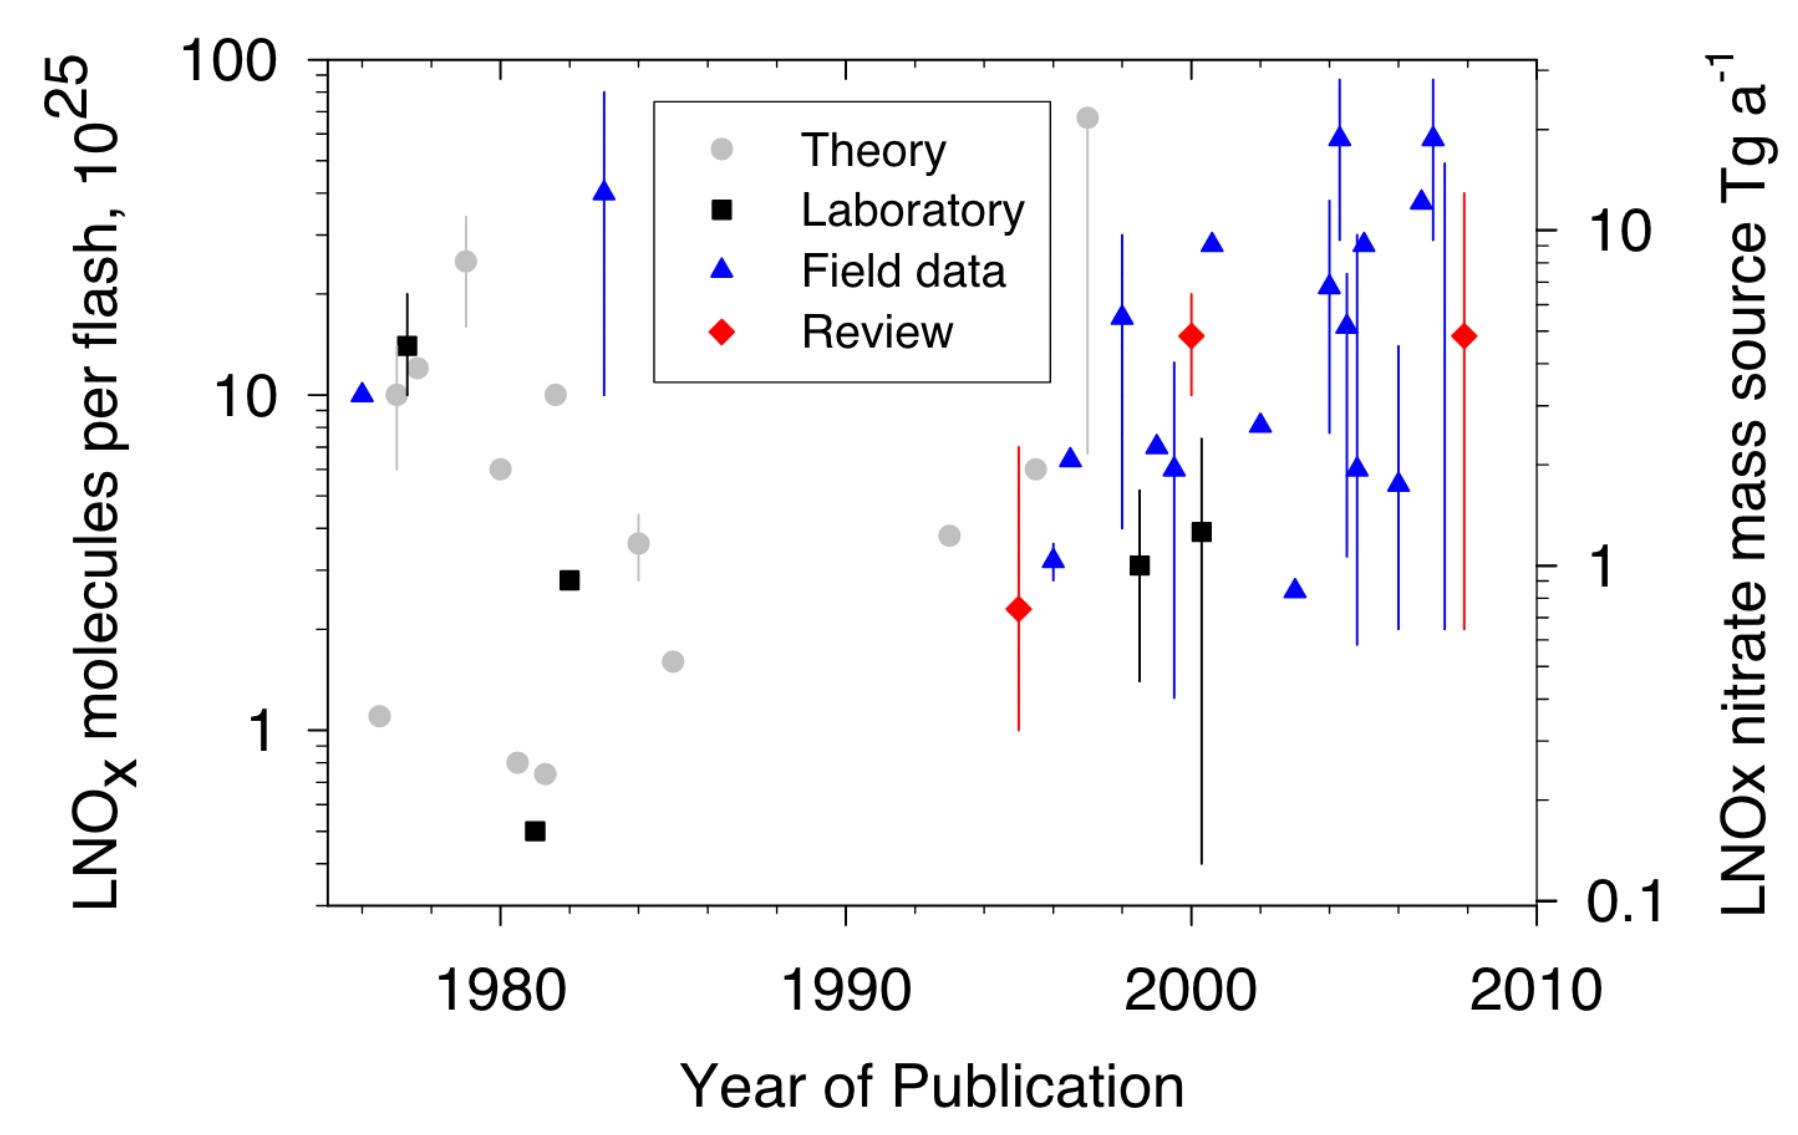
\includegraphics[width=0.7\textwidth]{./figures/lnox_production_Schumann.png}
\caption{不同年份的理论、实验室和外场观测以及综述中LNO$_x$的产率(10$^{25}$个分子)\\
Figure \ref{figure:lnox_production_Schumann}.
Flash-specific LNO$_x$ emissions in 10$^{25}$ molecules (NO$_x$ or NO) per flash from various theoretical, laboratory, and field studies and from reviews versus year of publication.
}
\label{figure:lnox_production_Schumann}
\end{figure}


假设全球上的雷暴数已知,则可以将单个雷暴估计得到的LNO$_x$产量外推至全球\citep{Chameides.1987,Huntrieser.1998,Huntrieser.2002}。
该方法需要测量出流区相对于入流区增加的NO$_x$浓度,以及雷暴的云砧出流区的质量通量,并估计全球任何时间活跃的雷暴数。
另一种方法是,根据每天发生的雷暴数量,估算闪电产生的NO$_x$量并将其推算到全球范围内\citep{Ridley.2004}。 这些方法的优点是,不需要任何闪电活动和云地闪产率比值的信息。
然而该方法需要提供准确的活跃雷暴数。研究表明,基于雷暴的外推结果值范围为0.3--13 Tg每年。
鉴于浓度(不确定因子1.5),出流通量或体积(不确定因子1.5)以及雷暴数(不确定因子1.5--2)的不确定性,
最佳估计值可能是5 Tg每年,其中不确定性因子约5,即估算值范围为1--25 Tg每年 \citep{Chameides.1987}。
虽然该方法对各种雷暴的性质提供了重要的支撑,但并没有降低全球LNO$_x$来源数值的不确定性。

鉴于NO$_x$在不同的对流区域寿命不一,而且LNO$_x$难以直接观测,因此夏季热带和中纬度地区的LNO$_x$仍需进一步研究。
由于NO$_2$在近紫外和可见光范围内具有独特的光谱吸收线,因此可以利用遥感对NO$_2$进行探测\citep{Platt.1983},
如全球臭氧监测实验[GOME; \citet{Burrows.1999}],
用于大气制图/化学的扫描成化学的扫描成像吸收光谱仪[SCIAMACHY; \citet{Bovensmann.1999}],
第二代全球臭氧监测实验[GOME-2; \citet{Callies.2000}]和臭氧监测仪[OMI; \citet{Levelt.2006}]。
最近于2017年发射的“哨兵-5P”卫星上搭载了对流层臭氧观测仪[TROPOMI; \citet{Veefkind.2012}],
其空间分辨率达到5.6 km $\times$ 3.6 km。
与传统平台相比,NO$_2$的卫星探测覆盖全球,仪器特征恒定且时间连续。

近年来,已有研究使用卫星观测确定并定量了LNO$_x$。
\citet{Beirle.2004}通过结合澳大利亚的GOME NO$_2$数据和闪电成像传感器(Lightning Imaging Sensor,LIS)数据,
将LNO$_x$限制在2.8(0.8--14) 吨氮每年。
\citet{Boersma.2005}通过比较GOME NO$_2$和第三代示踪剂模型(Tracer model 3, TM3)模拟的LNO$_2$分布估计全球LNO$_x$产量为1.1--6.4 吨氮每年。
\citet{Martin.2007a}用Goddard地球观测系统化学模型(GEOS-Chem)模拟分析了SCIAMACHY NO$_2$柱浓度,
将LNO$_x$估算为6 $\pm$ 2 吨氮每年。

这些方法侧重于每月或每年的平均NO$_2$柱浓度,而最近的研究采用特定方法直接探究活跃对流处的LNO$_x$。
\citet{Beirle.2006}基于墨西哥湾的对流系统,使用GOME NO$_2$柱浓度和美国国家雷电检测网络(NLDN)观测资料,估算LNO$_x$为1.7(0.6–4.7)吨氮每年。
然而,前提假设是增加的NO$_2$均来自闪电而无人为排放源的贡献。
\citet{Pickering.2016} 利用OMI和WWLLN算得LNO$_x$,该算法利用OMI对流层NO$_2$斜柱浓度作为LNO$_2$斜柱浓度,利用大于0.9的云辐射分数,来最小化或剔除对流层低层背景值。
该研究得出,2007--2011年夏季LNO$_x$产率为80 $\pm$ 45 mol每闪电。
在几个重要的不确定性来源中,该区域中的背景NO$_x$存在显著的不确定性(约3--30\%)。
% \citet{Zhang.2020b}使用气象和化学在线完全耦合的新一代区域空气质量模式(WRF-Chem),针对OMI卫星的NO$_2$产品,开发适用于估算污染地区LNO$_x$的新算法。
% 结果表明:该算法能将背景NO$_2$剔除,同时考虑处于云下的LNO$_2$,得出北美地区LNO$_x$产率为90$\times$50 mol NO$_x$ flash$^{-1}$。
图\ref{figure:lnox_production_xin}汇总了近十年不同方法所估算的LNO$_x$产率,
可见同一方法之间具有一致性,未来研究需要探讨不同方法之间差异的原因所在。

\begin{figure}[htbp]
\centering
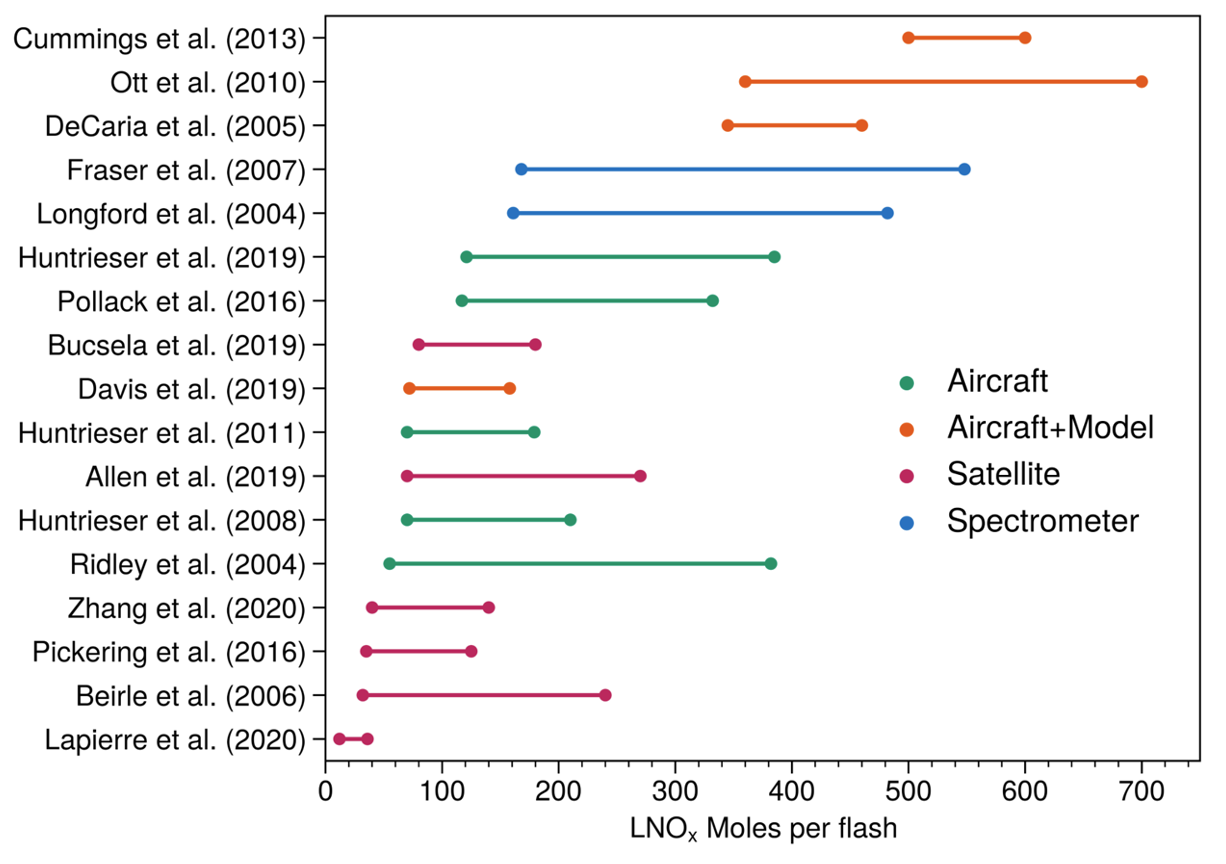
\includegraphics[width=0.8\textwidth]{./figures/lnox_production_xin.png}
\caption{近十年不同方法所估算的LNO$_x$产率\\
Figure \ref{figure:lnox_production_xin}. Estimates of LNO$_x$ production rate in the recent decade.}
\label{figure:lnox_production_xin}
\end{figure}

尽管模型模拟和卫星观测在对流研究中很普遍,但地面差分吸收光谱仪也很有价值,并已在一些研究工作中得到应用。
由于雷暴云中云粒子的米散射和化学反应,探测到的斜柱浓度会大大增加\citep{Erle.1995,Pfeilsticker.1998,Winterrath.1999}。
因此,光学路径可由差分光学吸收光谱(DOAS)\citep{Veitel.1998,Wagner.1998}和颜色指数得出,
其中颜色指数是两种不同波长下光强的比值,已被广泛用于云探测和云分类\citep{Wagner.2014,Wang.2015,Wagner.2016}。
另一方面,LNO$_x$可以使用同一仪器得出,但需要仔细地分离不同的来源。
\citet{Noxon.1976}根据以下几个假设,
1)所有观测到的NO$_2$都在云层和地面之间,
2)在分析时间内,闪电活动仍在进行,
3)NO$_2$没有明显损失,估算得到LNO$_x$产率的下限为:每个CG产生约10$^{26}$个NO$_2$分子。
由于光谱仪只能检测到NO$_2$,\citet{Franzblau.1989}利用了NO$_x$分析仪中NO与NO$_x$的比例,推算出每次闪电产生3$\times$10$^{27}$个NO$_x$分子。
最近,\citet{Langford.2004}重点研究了科罗拉多雷暴个例下部CG产生的NO$_x$,
并使用光谱测量和美国国家雷电探测网(NLDN)数据估算出每个CG生成5.8 $\pm$ 2.9$\times$10$^{26}$个NO$_x$分子。
值得注意的是,该光谱仪于777.4 nm处记录的闪电信息与OTD所用波段一样,包括IC和CG。
此外,在萨斯克彻温省的万斯科伊使用两台DOAS仪器,
开发了两种方法(NO$_2$与O$_4$的比例和特定的大气质量因子)来得出每次CG产生6.43--7.88$\times$10$^{26}$个NO$_2$分子
和每次总闪产生1.01--3.30$\times$10$^{26}$个NO$_2$分子\citep{Fraser.2007}。

目前我国针对LNO$_x$的研究较少,现有的工作主要是结合理论计算,估算局地LNO$_x$产量,
或分析局地NO$_x$ 浓度与雷暴活动的响应关系\citep{DuJian.2002,ZhangYiJun.2002,ZhouYunJun.2002},
对中国地区LNO$_x$年产量的估算不确定范围较大,达两个量级。
\citet{ZhouYunJun.2004}基于地闪定位网的闪电资料,通过假设单次闪电的能量,外推得到全国内陆LNO$_x$的产量为0.38 吨氮每年。
他们在估算中所用的地闪观测资料局限于广东、陇东、北京以及东北地区,存在一定的特殊性,
且在外推中选取的单次地闪能量为6.7$\times$10$^9$ J \citep{Price.1997a,Price.1997b},
该值为单次闪电产生能量的上限值 \citep{Wang.1998},因此,此估算值可能偏大。
\citet{SunAnPing.2004}基于 OTD 的总闪观测资料,假设单次闪电能量为4.5$\times$10$^7$ J,
没有考虑光学厚度对光能的影响及从光能到总能量的反演,因此该值比闪电本身的能量要小,
从而可能使其估算结果偏小,仅为0.016 吨氮每年。
近年来国内也有学者使用卫星观测来估算LNO$_x$,但是基于月平均或季平均数据且聚焦于清洁地区。
如通过分析青藏高原闪电活动和NO$_2$垂直柱浓度,发现LNO$_x$抑制了夏季青藏高原O$_3$低谷,且中国内陆地区LNO$_x$的年均产量为0.15(0.03--0.38)吨氮每年 \citep{JuXiaoYu.2015,Guo.2017,GuoFengXia.2019,Li.2022}。


% \subsection{深对流对痕量气体的垂直输送}
\subsection{深对流对痕量气体垂直分布的影响}

深对流云对大气化学成分的垂直输送,是近三十年来国际大气科学界一直高度关注的科学问题,
在TOGA-COARE\citep{Webster.1992}、TRACE-A\citep{Fishman.1996}和TRACE-P\citep{Jacob.2003}等一些重大国际合作项目中有关深对流的课题占了很大比重。
先后组织了一系列专门研究深对流云在大气化学成分再分布方面的大型综合观测试验,
其中包括于1998 年在欧洲进行的闪电与氮氧化物试验[EULINOX,\citet{Holler.2000}]、
2002 年在佛罗里达进行的CRYSTAL-FACE 试验\citep{Toon.2003}、
2003至2005年在巴西实施的欧共体项目TROCCINOX\citep{Huntrieser.2008},
以及2012年在美国进行的深对流云和化学试验[DC3,\citet{Barth.2019}]等。
在这些试验中,深对流云对气溶胶及其主要前始气体以及闪电对对流层上层NO$_x$和O$_3$浓度的影响是研究的重点。
与此同时,各种尺度和复杂程度的数值模式也用来模拟和解释外场观测结果。

深对流输送边界层痕量气体至UTLS的能力,取决于各种气象和化学要素。
在1985年PRESTORM的风暴尺度观测项目中,由于深对流输送对流层上层一氧化碳(CO)浓度显著增加\citep{Dickerson.1987,Pickering.1989}。
然而,在6月17日的个例中,对流层上层出流区的CO混合比与背景水平相似。这是由于冷锋过境并阻止了边界层空气直接进入云层,从而边界层上方的空气主导了入流区\citep{Pickering.1988}。
因此,天气尺度背景在深对流输送作用中起着重要作用。

除天气尺度背景外,边界层条件和动力结构也影响着深对流的输送效率。
1989年北达科他州雷暴观测项目中的中尺度对流复合体(MCC)的模拟结果表明,边界层越潮湿,对流输送能力越强,从而更多的CO被输送至云砧\citep{Stenchikov.1996}。
其他一些对流个例研究表明,深对流的输送能力与对流的垂直速度以及传输速度密切相关\citep{Pickering.1992a,Wang.1996}。
\citet{Bigelbach.2014}通过模拟2007年美国南部大平原对流季节的传输,发现准绝热强对流(QISC)比中尺度对流系统(MCSs)具有更强和更深的通量,即不同类型的对流系统具有不同的输送能力。
\citet{Li.2017b}通过对比热泡对流,超级单体和MCS三种不同类型的对流系统,发现超级单体的痕量气体输送能力最强。
这是由于超级单体受质量通量的垂直梯度影响更大,而不是痕量气体混合比的垂直梯度。

入流区的结构也影响着深对流的输送能力。针对美国国家航空航天局(NASA)亚马逊边界层实验(ABLE)的观测,
\citet{Scala.1990}使用二维云模型研究了热带飑线内空气的运输途径。
气团轨迹分析表明,输送到云砧的空气中有50\%以上来自对流层中部(6 km或以上),而不是边界层。
进入对流核上升气流的空气中,50\%以上的气团被限制于5 km以下,仅约15\%的边界层空气直接传输至12 km附近的云层。
另一方面,在亚马逊干旱季节,巴西生物质燃烧区的对流个例显示,大量的O$_3$前体物被垂直输送至对流层上层,导致对流层上层O$_3$的产生大量增加\citep{Pickering.1992,Pickering.1992a,Pickering.1996}。
湿季和干季等效位温垂直廓线的巨大差异,导致对流输送特性的差异。针对中纬度地区的个例研究表明,大部分输送至UTLS的气团来源于边界层\citep{Mullendore.2005,Skamarock.2000}。

在深对流输送研究中,云参数化和云分辨模型均具有广泛应用。深对流对痕量气体的传输模拟需要真实地再现天气尺度背景、边界层结构、对流演变过程、入流区结构以及周围的化学成分。 气象研究与预报(WRF)模型是为气象研究和数值天气预报设计的三维可压非静力大气模型。气象与化学耦合模式(WRF-Chem)是结合了大气化学的WRF模型,可以同时模拟气象学中痕量气体和气溶胶的排放、传输、混合和化学反应\citep{Fast.2006,Grell.2005}。
\citet{Barth.2012}首次在整个美国大陆上以高分辨率(4 km)应用WRF-Chem模型,研究北美季风早期阶段的对流输运和化学反应。
之后,许多研究利用WRF和WRF-Chem模拟从边界层到对流云砧区的输送个例\citep{Bela.2016,Li.2017b,Li.2018}。
痕量气体的次网格对流传输是云参数化模拟的重要组成部分。
\citet{Wang.1996}针对TRACE-A观测的热带MCS和PRESTORM观测期间的飑线,利用多层嵌套探讨了次网格尺度和网格尺度对流传输的差异。
其中MCS个例使用90和30 km两层嵌套,飑线个例使用75和25 km两层嵌套。
研究发现,在上升气流中发生了大量的次网格传输(在MCS个例中约占总向上传输的41\%,在飑线个例中约占64\%)。
\citet{Ott.2009}将云分辨模式(CRM)和柱模式(SCM)对三种对流系统中痕量气体垂直分布的模拟结果进行了比较。
他们发现,相对于CRM,SCM低估了对流层上部的对流质量通量和痕量气体混合比。
此外,他们也研究了SCM中对流传输对微物理方案参数值的敏感性。
通过调整影响对流传输的最重要参数,改进了SCM对痕量气体混合比的模拟。
\citet{Freitas.2000}针对低分辨率大气模式,提出了与深对流系统相关的次网格痕量气体对流输送的参数化。
\citet{Grell.2014}详细描述了次网格对流参数化,示踪气体传输和湿清除计算方法,该方法可用于高分辨率非静力中尺度模式。
\citet{Li.2018}通过对比不同的对流参数化(12和36 km)和云分辨模拟结果,
指出对流参数化模拟的对流输送比云分辨模拟结果要弱,并且该输送能力在对流早期而不是后期受对流参数化的控制更多。
因此,对流输送参数化与次网格对流云方案需一致,且对流参数化需要能够真实反映冰相的微物理。

在对流层上层中形成的O$_3$和气溶胶的多少,取决于净对流输送的液相和/或冰相中可溶并具有反应性的气体。
在对流层上层中,O$_3$的形成需要NO$_x$和HO$_x$,其机理为HO$_2$和有机过氧自由基(RO$_2$)将NO氧化,
然后NO$_2$光解,激发态O原子与O$_2$分子结合。
但是,由于HO$_x$的寿命短,因此对流层上层中HO$_x$的量取决于寿命更长的HO$_x$前体物的含量\citep{Chatfield.1984,Prather.1997},
例如过氧化氢(H$_2$O$_2$),甲基过氧化氢(CH$_3$OOH)和甲醛(CH$_2$O),
这些前体物是可溶的,且具有液相的化学源和汇\citep{Barth.2007,Carlton.2007}。
H$_2$O$_2$是由HO$_2$自由基与其自身反应形成的。 CH$_2$O和CH$_3$OOH来自于CH$_4$和其他碳氢化合物的氧化。
对流层上层的NO$_x$除了来源于LNO$_x$,也受对流输送的边界层NO$_x$以及硝酸(HNO$_3$)影响\citep{Grassian.2005},
而HNO$_3$很容易被云水和冰粒清除\citep{Neu.2012}。
通过比较DC3项目中入流区和出流区内的痕量气体,可知CH$_3$OOH的清除效率(12--84\%)很大程度上取决于冰相保留系数,
但H$_2$O$_2$(80--90\%)和CH$_2$O(40--60\%)并非如此\citep{Barth.2016,Bela.2016,Fried.2016}。
\citet{Cuchiara.2020}指出,与SEAC4RS观测中CH$_3$OOH清除率(4\%--27\%)相比,DC3观测中其清除率更高,该现象很大程度上可由冰相保留系数解释。
有关DC3项目的研究总结(如垂直输送,湿清除,LNO$_x$,平流层-对流层交换等)详见\citet{Barth.2019}。

我国的研究人员在深对流云对污染物的垂直输送方面也做了有意义的探索。
\citet{GaoHuiWang.1998}利用一个欧拉型硫沉降模式,研究了积云对硫污染物垂直输送的作用。
他们的结果表明,积云引起的垂直气流可使对流层高层的硫污染物浓度增加50--400\%。
\citet{LiBing.1999,LiBing.2001}则利用一个耦合的冰雹云-化学模式模拟了
我国陕西一次单体积云对流的发展过程及其对对流层O$_3$和NO$_x$等化学成分再分布的作用。他们的模拟结果表明,
云内强烈的垂直输送能在30分钟左右把低层低体积分数的O$_3$和高体积分数的NO$_2$快速、
有效地输送到对流层的上部,造成化学物种的再分布。
\citet{HuJiaYing.2019}利用带有详细分档微物理方案及液相化学的云模式,
对2014年7月30日发生在安徽滁州境内一次深对流过程进行了模拟研究。
研究结果表明,在积云发展阶段,强上升气流使得云内源层示踪气体有效地向上输送,
对流层中部强的夹卷过程及水平入流使得云外气体入云输送至主要对流区,并在垂直气流的作用下进一步影响各层示踪气体的分布。
各层示踪气体均可向上输送至对流层上部,其中对流层中部示踪气体(2.1--4.5 km、4.5--7.5 km 和 7.5--10.8 km)的向上输送作用与近地层示踪气体(0--2.1 km)的贡献相当。

% \subsection{闪电氮氧化物的影响}



\section{存在问题及本研究目标和研究内容}

总体而言,我国在大气污染物垂直输送及相关物理化学过程和机制方面的研究还很少,即使有,也比较零散,
特别是缺少对对流输送相关事实的观测认知,这与近几年开展较多的地面大气污染观测和模拟研究不相称。
所以,进行对大气污染物垂直输送过程、机理及其影响的研究,对全面理解和预测其环境、气候效应都具有不可替代的作用。
而探索闪电对对流层上层NO$_x$和O$_3$产量的贡献,是理解深对流云对大气成分垂直分布影响的另一个重要方面。

具体而言,有以下科学问题亟待研究:

\begin{enumerate}[label=(\arabic*), labelindent=\parindent, leftmargin=0pt, widest=0, itemindent=*, topsep=0pt, partopsep=0pt, parsep=0pt]

\item 由于原位观测有限,如何利用卫星资料得到不同地区的LNO$_2$柱浓度和产率?

\item LNO$_2$的产率与哪些因素有关?对闪电NO$_x$的产量有何影响?

\item 除了LNO$_2$柱浓度,能否利用卫星资料得到对流云的NO$_2$和O$_3$廓线并进行来源分析?

\item 针对不同的深对流系统,动力输送和化学反应如何影响O$_3$的垂直再分布?其中LNO$_x$又起到了什么作用?

\end{enumerate}

针对以上问题,本文的研究目标为:

\begin{enumerate}[label=(\arabic*), labelindent=\parindent, leftmargin=0pt, widest=0, itemindent=*, topsep=0pt, partopsep=0pt, parsep=0pt]

\item 利用更准确的NO$_2$先验廓线,开发适用于清洁和污染地区的LNO$_2$柱浓度产品,进而估算LNO$_2$的产率。

\item 将卫星得到的多种二级产品与闪电数据相结合,分析闪电NO$_x$的产率与云属性和闪电属性的关系。

\item 将前人的云切片算法用于不同高度的对流云,探讨其适用条件和得到的NO$_2$和O$_3$廓线分布,
并与模拟结果进行对比分析从而确认差异来源。

\item 针对中国地区不同的深对流系统开展联合观测,为模式模拟提供可靠数据(雷达产品、闪电定位信息以及O$_3$廓线),
并利用评估后的模式来进一步研究动力输送、化学反应和LNO$_x$的作用。

\end{enumerate}

本文研究内容与章节安排如下:

第一章:阐述本文的选题依据和意义,从原位观测、模式模拟以及卫星观测的角度回顾了
1)深对流云对大气化学成分的垂直输送,
2)闪电NO$_x$的产率估算及其对其他痕量气体的影响,
提出本文的科学问题和研究内容。

第二章:介绍本文的资料来源和研究方法,对论文中使用的模式和反演方法进行简要介绍。

第三章:开发适用于不同地区的LNO$_2$算法,分析北极、美国大陆以及中国污染地区的LNO$_2$产率,并与其他NO$_x$排放源进行对比。
分析LNO$_2$产率与海陆差异和闪电频率之间的关系,并量化其对LNO$_2$产量的影响。

第四章:将云切片算法得到的NO$_2$廓线与相同条件下模式模拟的NO$_2$廓线进行对比分析,并利用模式的敏感性试验探讨LNO$_2$对NO$_2$柱浓度的重要性。

第五章:利用已得的NO$_2$廓线和模式结果,分析云切片算法得到的不同地区O$_3$垂直分布。
此外对中国东南部的联合观测试验进行说明,并利用模式具体分析不同类型的深对流系统对O$_3$的影响,
得到动力输送、化学反应及LNO$_x$在其中所起的作用。

第六章:对全文进行总结,提炼结论,并讨论论文的创新点并探讨研究的不足之处以及对于未来工作的展望。

	%!TEX root = ../thesis.tex

\chapter{资料及模式介绍}

\section{原位观测}

\subsection{臭氧探空}

针对中国东南部的强对流天气,于2019年7月25日和2020年9月1日,
在南京国家基准气候站(31.93$^{\circ}$ N,118.90$^{\circ}$ E)共释放了五个臭氧探空仪。
为了研究对流的影响,我们分别在对流发生前和对流发生中/对流发生后各释放一次探空。
深对流概况及臭氧探空仪轨迹见图\ref{fig:ozonesonde}。

\begin{figure}[H]
\centering
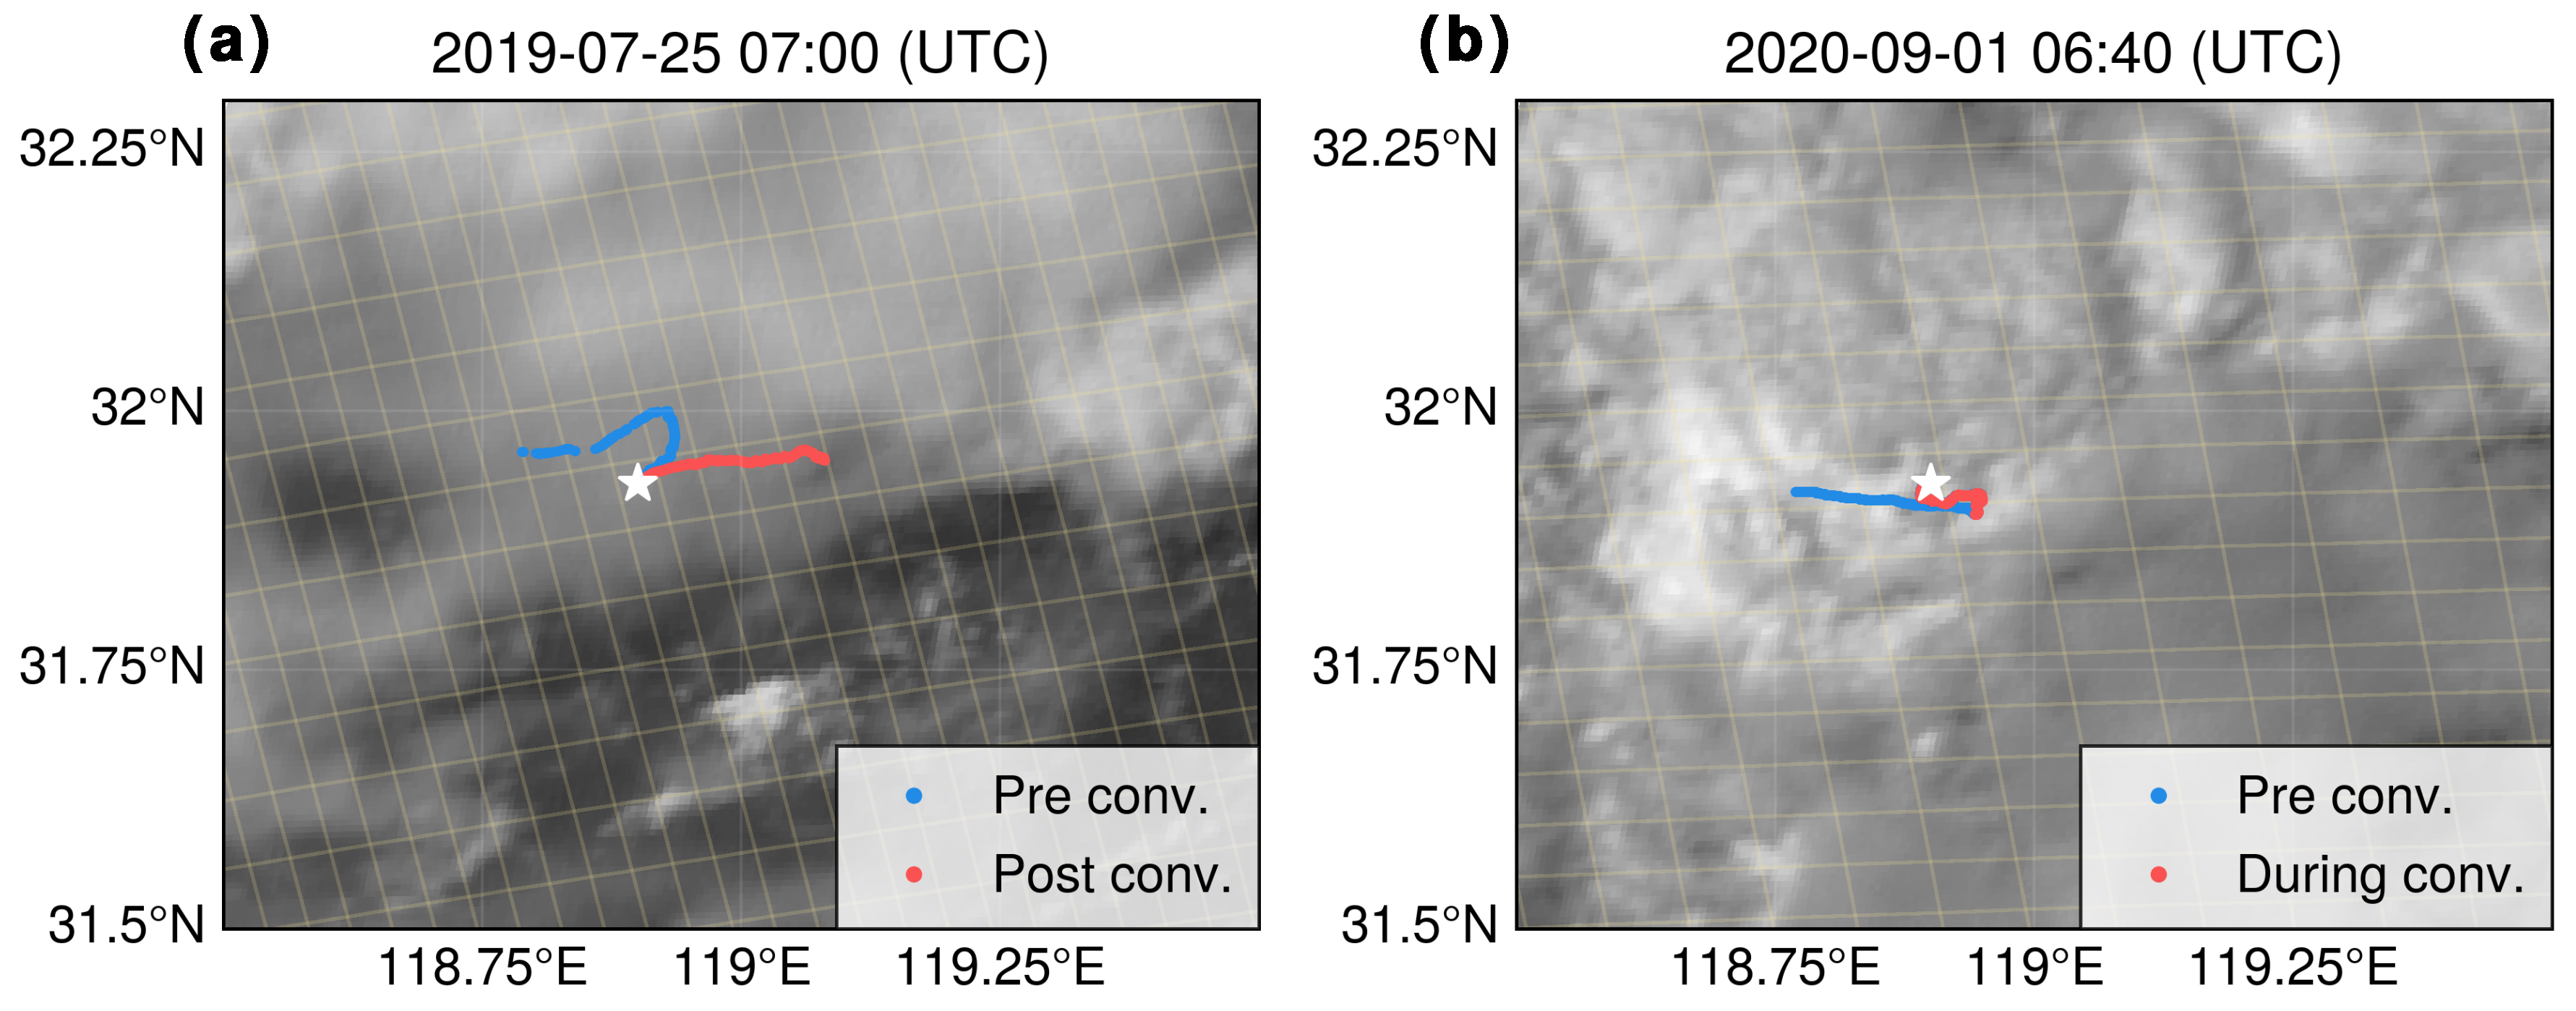
\includegraphics[width=0.9\textwidth]{./figures/ozonesonde.png}
\caption{在对流后或对流中的臭氧探空仪达到约 10 km时,风云4A先进地球静止辐射成像仪(AGRI)可见通道(0.65 $\mu$m)探测到的对流。
对流前的臭氧探空仪轨迹为蓝色,其他为红色。白星符号代表观测站,细黄线是TROPOMI像素条带。\\
Figure \ref{fig:ozonesonde}. The convection detected by the FY-4A Advanced Geostationary Radiation Imager (AGRI)
visible channel (0.65 $\mu$m) field at the time when the post-convection/during-convection ozonesondes reached around 10 km.
The pre-convection ozonesonde trajectories are colored blue while others are in red.
The white star symbol stands for the observation station and the thin yellow lines are the TROPOMI swath pixels.
}
\label{fig:ozonesonde}
\end{figure}


具体而言,2019年7月25日发生的对流为热对流,释放的三个臭氧探空均产自中国大气物理研究所(IAP)。
IAP 臭氧探空仪使用电化学浓差电池(ECC),其完整参数和性能见\citet{Zhang.2014}。
就性能而言,从地表到2.5 km平均偏差小于0.3 mPa,9 km以下接近零,9--18 km之间小于0.5 mPa。
第一台IAP臭氧探空仪于7月23日(晴天)05:35 UTC释放,另外两台分别于7月25日05:10 UTC(对流前)和06:35 UTC(对流后)释放。
由于防水故障,对流前释放的探空仪在释放后几秒钟就失去了信号,故而我们选择了7月23日释放的臭氧探空仪作为对流前的数据。
虽然时间间隔为2天,但10 km以上预报的O$_3$廓线最大相对差异通常小于25\%(图\ref{fig:waccm_forcast_o3}),
因此O$_3$日变化不足以解释探空观测到的超过65\%的差异。

此外,两台维萨拉(VAISALA)ECC臭氧探空仪分别于8月31日23:45 UTC(对流前)和9月1日06:10 UTC(对流期间)成功释放。
准备工作及具体操作均遵循标准手册,确保精度优于5\%,且30 km 以下的精度在$\pm$(5--10)\% 以内\citep{Smit.2007}。
该次探空试验所捕获的飑线是由冷空气和台风梅萨克(Maysak)外围环流的汇合发展而来的。
值得强调的是,对流期间的臭氧探空仪直接穿入云层,为探索受对流云影响的O$_3$提供了独特的机会。

\begin{figure}[H]
\centering
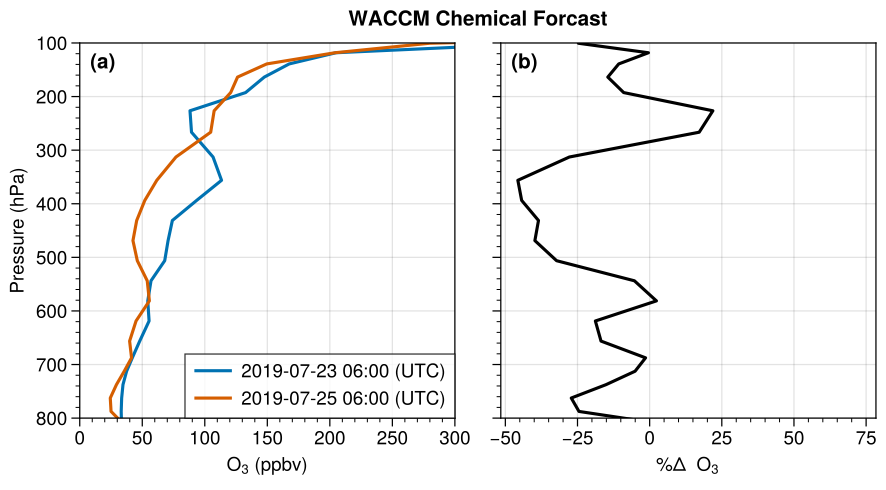
\includegraphics[width=0.8\textwidth]{./figures/waccm_forcast_o3.png}
\caption{(a)全大气层气候模型(WACCM)预报场的区域平均(118.5--119.5$^{\circ}$ E, 31.5--32.5$^{\circ}$N)O$_3$廓线。
蓝色为对流前,橙色为对流后。(b)为(a)中O$_3$廓线的百分比差异。\\
Figure \ref{fig:waccm_forcast_o3}. (a) Regional mean (118.5$^{\circ}$E – 119.5$^{\circ}$E, 31.5$^{\circ}$N – 32.5$^{\circ}$N)
pre-convection (blue) and post-convection (orange) O$_3$ profiles from the 6-hour Whole Atmosphere Community Climate Model (WACCM) forecasts.
(b) The percent difference of O$_3$ profiles in (a).
}
\label{fig:waccm_forcast_o3}
\end{figure}

\subsection{闪电数据集}

在\ref{sec:arctic}节北极的研究中,我们使用了维萨拉全球雷电数据集(GLD360)。
该闪电探测网建立于2009年,由全球极低频闪电探测传感器组成,可检测CG和IC\citep{Said.2010,Said.2013,Said.2017},
CG和IC在北极洋面上的探测效率分别为50--60\% 和 < 10\%\citep{Vagasky.2022}。
因此,我们使用恒定的云闪地闪比率($\sim$1)来计算总闪,
即修正后的总闪击为检测到的地闪闪击的4倍\citep{Mackerras.1994,Prentice.1977}。
该常数比是根据两个要素计算的:每次闪电的闪击数(闪电多重性)和高纬度地区IC与CG闪击数的平均比(也称为Z比例)。
闪电多重性对探测效率和将闪击重组为闪电的算法较为敏感\citep{Schulz.2005,Yair.2014,Burgesser.2017,Kolmasova.2022},
\citet{Yusop.2019}的高纬度闪电研究表明闪电多重性约为1.2。
此外,高纬度闪电的平均Z比例在 1 到 1.3 之间\citep{Mackerras.1994,Prentice.1977,Bandholnopparat.2020}。
为了评估使用常数比的敏感性,我们在研究中设置了不同的值(1:2 和 2:1)来评估得到的LNO$_x$排放量的不确定性。


在\ref{sec:us}节美国大陆的研究中,我们使用了整体闪电探测网(ENTLN)。
ENTLN运营着一个由全球1500多个地面站组成的系统,在美国大陆安装有900多个传感器\citep{Zhu.2017,Marchand.2019}。
CG和IC均由传感器根据电场脉冲极性和波形进行定位,检测频率范围为1 Hz 至 12 MHz。
如果脉冲组在700 ms和10 km范围内,它们则被归类为闪电。
在ENTLN的预处理数据中,包括了闪击和由一个或多个闪击组成的闪电。
\citet{Rudlosky.2015}将ENTLN组合事件(CG和IC)与LIS测得的闪电进行了比较,
发现ENTLN在美国大陆上的闪电探测效率从2011年的62.4\%增加到2013年的79.7\%。
\citet{Lapierre.2020}还将 ENTLN 和 NLDN 数据集与2014年LIS的数据进行了比较,发现IC闪电和闪击的探测效率分别为88\% 和 45\%。
由于我们和\citet{Lapierre.2020}一样仅使用2014年的ENTLN数据,故采用同样的方法得到总闪的量:
IC闪电数除以0.88,IC闪击数除以0.45,而CG由于探测效率高,故不进行矫正。

在\ref{sec:china}节中国东南部的研究中,我们融合了三种闪电数据集:中国国家闪电探测网[CNLDN,\citet{Yang.2015}]、
ENTLN和全球闪电定位网[WWLLN,\citet{Rodger.2006}]。
江苏省CNLDN数据的地闪闪电探测效率约为90\% \citep{Li.2017a},
而ENTLN和WWLLN以特定的频率(ENTLN 为 1 Hz -- 12 MHz,WWLLN 为 3--30 kHz)同时探测IC和CG,
WWLLN的详细处理算法由\citet{Rodger.2004}给出。
在 10 km 和 0.7 s的条件下,WWLLN测得的闪击和脉冲与ENTLN融合,构成一个数据集[ENGLN,\citet{Virts.2020b}]。
为了增加我们研究中的闪电数据覆盖范围,使用 10 km 和 0.5 s 的时空聚类标准将ENGLN和CNLDN数据集的地闪数据相结合\citep{Zhao.2020},合并后的数据集应具有足够高的地闪探测效率。
由于这三种闪电数据集在中国范围内的云闪探测效率较低,
我们保守地使用恒定的IC与CG比例(3:1)来得到总闪数据\citep{Wu.2016,Bandholnopparat.2020}。
若将来中国有更多如北京闪电网络[BLNET,\citet{Srivastava.2017}]的闪电网,
则可利用这些新数据与闪电成像传感器进行比较\citep{Rudlosky.2013,Poelman.2020},从而得到更加准确的IC数据。

\section{卫星观测}

\subsection{臭氧监测仪(OMI)}

OMI搭载在Aura卫星(2004年发射)上,该卫星是下午列车(A-train)卫星组的成员\citep{Levelt.2006,Levelt.2018}。
OMI在当地时$\sim$13:45(升交点)经过赤道,在 705 公里的高度以 98.2$^{\circ}$ 的倾角运行,幅宽为2600 km,最高分辨率为13 km $\times$ 24 km。
OMI是一种紫外/可见光光谱仪,光谱范围在270--500 nm,光谱分辨率约为0.5 nm,可用来观测NO$_2$、SO$_2$、HCHO、BrO 和 OClO等痕量气体。
OMI 使用二维探测器,其中在探测器的一个轴上对跨轨道地面像素进行成像,在另一个轴上记录光谱信息。 这种传感技术允许同时测量条带中的所有地面像素,因此OMI 没有扫描镜,且该二维检测器可实现宽幅、良好空间分辨率和高信噪比的组合。
OMI采用DOAS拟合来确定NO$_2$和O$_3$的垂直柱浓度,其中NO$_2$数据通常用于研究城市空气污染,评估NO$_x$排放源的影响,监测NO$_2$污染物的变化趋势等。
OMI的观测数据可以与其他大气环境监测仪器数据相结合,共同为研究者提供更全面的大气环境数据。

然而自2007年初以来,由于被称为“行异常”的异常辐射\citep{Dobber.2008},一些测量数据变得无效。
对于当前的研究,我们使用NASA标准产品v3.0\citep{Krotkov.2017}作为LNO$_x$反演算法的输入。

对流层NO$_2$垂直柱浓度($V_{\ch{NO2}}$)的计算主要包括以下步骤:

\begin{enumerate}[label=(\arabic*), labelindent=\parindent, leftmargin=0pt, widest=0, itemindent=*, topsep=0pt, partopsep=0pt, parsep=0pt]

\item NO$_2$总斜柱浓度由 OMI 优化的DOAS拟合确定。

\item 通过从测量的总斜柱浓度中减去由仪器引起的跨道偏差,得到校正(“去条纹”)的总斜柱浓度。

\item 平流层和对流层的大气质量因子($AMF_{\ch{strat}}$,$AMF_{\ch{trop}}$)是由考虑加权散射权重的NO$_2$先验廓线的垂直积分计算得到。
这些先验廓线是GMI模式模拟的月平均先验廓线(2004--2007 年)。

\item 平流层NO$_2$垂直柱浓度($V_{\ch{strat}}$)是通过减去对流层NO$_2$的先验贡献和三步算法(插值、过滤和平滑)计算得出\citep{Bucsela.2013}。

\item $V_{\ch{strat}}$ 使用 $AMF_{\ch{strat}}$ 转换为斜柱浓度,并从测量的总斜柱浓度中减去,从而得到对流层NO$_2$斜柱浓度($S_{\ch{NO2}}$),进而 $V_{\ch{NO2}}$ = $S_{\ch{NO2}}$/$AMF_{\ch{trop}}$。

基于这种方法,我们开发了$AMF_{\ch{LNO_x}}$,通过替换原来的步骤来获得所需的LNO$_x$垂直柱浓度 $V_{\ch{LNO_x}}$($V_{\ch{LNO_x}}$ = $S_{\ch{NO2}}$/$AMF_{\ch{LNO_x}}$),该算法的具体细节将在\ref{sec:amf_definition}节中讨论.

\end{enumerate}

\subsection{对流层观测仪(TROPOMI)}

2017年10月13日,搭载TROPOMI的哨兵5号(Sentinel-5 Precursor)卫星成功发射\citep{Veefkind.2012},于每日当地时间13:30左右经过赤道。
TROPOMI提供在四个通道(紫外、可见光、近红外和短波红外)中测量各种痕量气体浓度,以及云和气溶胶特性。
在用于NO$_2$反演的可见光通道(400–496 nm)中,光谱分辨率和采样分别为 0.54 和 0.20 nm,信噪比约为 1500。
单个地面像素为7.2 km(2019年8月6日之后为5.6 km),沿着轨迹的积分时间为1.08 s(0.84 s),在条带中间的跨轨迹方向为 3.6 km。
轨道上有450个地面像素(行),它们的大小朝向条带边缘或多或少保持不变(最大像素宽约14 km)。
扫描幅宽约为2600 km,TROPOMI每天都实现全球覆盖,除了赤道处约0.5$^{\circ}$宽度的轨道之间的窄带。
由于处理中太阳天顶角($\theta_0$ $\leq$ 88$^{\circ}$)的限制,约有15\%的地面像素未处理。

在非常明亮的辐射场景(例如高云)中,包含波段4(可见;例如用于NO$_2$反演)和波段6(近红外;例如用于云数据反演)的电荷耦合器件(CCD) 探测器可能会出现饱和效应\citep{Ludewig.2020},导致某些光谱(即波长)像素的辐射率低于预期。
在饱和度大的情况下,可能会发生电荷溢出:过量电荷从饱和的行方向流入相邻的像素,导致某些光谱像素的辐射率高于预期。
1.0.0版的1b级光谱包含饱和度标记,但不包含溢出标记;2.0.0 版开始有溢出标记\citep{Ludewig.2020}。
对于本文的研究,我们使用Sentinel-5P产品算法实验室(S5P-PAL)再处理产品(v2.3.1)。
与v1.2/v1.3版本相比,新版本的产品包含了尖峰去除功能,以更好地处理探测器的饱和效应,从而在明亮的对流云层上提供更多有效的数据\citep{Ludewig.2020,VanGeffen.2022},
其中具有较大反演误差(processing\_quality\_flags > 0)的像素被过滤掉。

与OMI一样,$AMF_{\ch{trop}}$取决于多个参数(太阳天顶角、视角天顶角、相对方位角、表面反照率、地表气压、云分数、云高度和先验廓线):
\begin{equation} \label{eq:AMF_NO2}
AMF_{\ch{trop}} = \frac{(1-f_r) \int_{p_{surf}}^{p_{tp}} w_{clear}(p) NO_2(p) \: dp + f_r \int_{p_{cloud}}^{p_{tp}} w_{cloudy}(p) NO_2(p) \: dp}{\int_{p_{surf}}^{p_{tp}} NO_2(p) \: dp}
\end{equation}
简而言之,分子是模拟的$S_{\ch{NO2}}$,分母是模拟的$V_{\ch{NO2}}$。
其中$p_{surf}$是表面气压,$p_{tp}$是对流层顶气压,$p_{cloud}$是云压,$f_{r}$是NO$_2$窗区中的云辐射率分数,
$w_{clear}$和$w_{cloudy}$分别是查找表中的气压相关散射权重\citep{Lorente.2017},
$NO_2(p)$是示踪剂模式第五版(TM5)模拟的NO$_2$垂直廓线。

云压是由477 nm附近O$_2$--O$_2$碰撞吸收带反演得到的反射率加权气压\citep{Acarreta.2004,Sneep.2008,Stammes.2008},
故深对流云的云压位于几何云顶下方,
其中几何云顶与云探测卫星(CloudSat)和中分辨率成像光谱仪(MODIS)等热红外传感器检测到的值更接近\citep{Vasilkov.2008,Joiner.2012}。
因此,OMI或TROPOMI测量的对流层NO$_2$大部分位于云内部,而不是云顶之上。
下文中,“云上”或“云下”都是相对于OMI或TROPOMI测得的云压而言。
\citet{Beirle.2009}的敏感性研究比较了云底和云顶的化学成分,发现云中大部分LNO$_2$可以被卫星探测到。
云压的概念不仅应用于LNO$_x$的研究,还应用于计算对流层上层O$_3$和NO$_x$的云切片方法\citep{Ziemke.2009,Choi.2014,Strode.2017,Ziemke.2017,Marais.2018}。


\subsection{微波临边探测器(MLS)}

MLS搭载在Aura卫星上,在当地时$\sim$13:45(升交点)经过赤道。
MLS是一种热发射微波临边探测仪,可测量中间层、平流层和对流层上层温度、O$_3$和其他几种痕量气体的垂直剖面。
MLS仪器主要使用240 GHz 微波波段进行O$_3$反演,在 38 个气压层上(0.0215--261 hPa)具有有效的科学数据。
这些层的垂直间距在1 hPa 以下各处约为1.3 km,在 1 hPa 以上的大多数高度约为 2.7 km。
相比之下,O$_3$反演的垂直分辨率为$\sim$3 km,从 261 hPa 向上延伸到中间层。
本研究中使用的MLS O$_3$廓线数据(5.0版本)的时间段为2019年6月至8月,为了与OMI和TROPOMI匹配,我们仅使用白天的O$_3$廓线数据。
由于本文研究对象为对流云,我们参考\citet{Livesey.2013}利用冰水含量(IWC)来获得对流云条件的有效O$_3$廓线数据。
MLS的IWC产品与O$_3$数据一样,是基于 240 GHz 光谱区域(~1.2 mm)的观测结果。
在此波长下只能观察到具有大粒径的厚云[215 hPa高度的IWC $>$ 0.6 mg m$^{-3}$ \citep{Wu.2008}]。 这种云通常与深对流核有关,而不是外流或局地形成的卷云。
因此,MLS IWC在本研究中用作深对流的量度,其有效范围为 215--83 hPa。
IWC加权函数的分析表明,215 hPa高度IWC的垂直分辨率约为4 km\citep{Wu.2008}。
\citet{Livesey.2013}采用迭代拟合算法以去除IWC产品中的一些残余晴空信号。
具体来说,这涉及计算IWC产品的每日 10$^{\circ}$纬向均值,反复剔除大于均值两个标准差的数据,
并在每次迭代中重新计算剩余总体的均值和标准差$\sigma$。
一旦该方法收敛(通常在5--10次迭代内),任何大于 3$\sigma$ 的 IWC值都被认为是具有统计显著性的对流云并包含在平均值中(去除了纬向平均“背景”)。
此外我们使用MLS O$_3$的数据质量标志来进一步提取有效数据:准确度 $>$ 0、状态为偶数、数据质量 $>$ 1.0以及收敛度 $<$ 1.03。


\subsection{闪电氮氧化物的计算} \label{sec:amf_definition}

基于$AMF_{\ch{trop}}$,为了得到对流层LNO$_2$或LNO$_x$的垂直柱浓度,我们只需将分母改成LNO$_2$或LNO$_x$的垂直积分即可。
\begin{equation} \label{eq:AMF_LNO2}
AMF_{\ch{LNO_2}} = \frac{(1-f_r) \int_{p_{surf}}^{p_{tp}} w_{clear}(p) NO_2(p) \: dp + f_r \int_{p_{cloud}}^{p_{tp}} w_{cloudy}(p) NO_2(p) \: dp}{\int_{p_{surf}}^{p_{tp}} LNO_2(p) \: dp}
\end{equation}

当研究区域为清洁区域,式(\ref{eq:AMF_LNO2})的分子可用LNO$_2$代替NO$_2$,即
\begin{equation} \label{eq:AMF_LNO2clean}
AMF_{\ch{LNO_2Clean}} = \frac{(1-f_r) \int_{p_{surf}}^{p_{tp}} w_{clear}(p) LNO_2(p) \: dp + f_r \int_{p_{cloud}}^{p_{tp}} w_{cloudy}(p) LNO_2(p) \: dp}{\int_{p_{surf}}^{p_{tp}} LNO_2(p) \: dp}
\end{equation}

为了与前人对比,我们定义了其他两种云上的AMF,
\begin{equation} \label{eq:AMF_NO2Vis}
AMF_{\ch{NO_2Vis}} = \frac{(1-f_r) \int_{p_{surf}}^{p_{tp}} w_{clear}(p) NO_2(p) \: dp + f_r \int_{p_{cloud}}^{p_{tp}} w_{cloudy}(p) NO_2(p) \: dp}{(1-f_g) \int_{p_{surf}}^{p_{tp}} NO_2(p) \: dp + f_g \int_{p_{cloud}}^{p_{tp}} NO_2(p) \: dp}
\end{equation}
\begin{equation} \label{eq:AMF_LNO2Vis}
AMF_{\ch{LNO_2Vis}} = \frac{(1-f_r) \int_{p_{surf}}^{p_{tp}} w_{clear}(p) NO_2(p) \: dp + f_r \int_{p_{cloud}}^{p_{tp}} w_{cloudy}(p) NO_2(p) \: dp}{(1-f_g) \int_{p_{surf}}^{p_{tp}} LNO_2(p) \: dp + f_g \int_{p_{cloud}}^{p_{tp}} LNO_2(p) \: dp}
\end{equation}
其中$f_g$为云几何分数。以上各式中的NO$_2$和LNO$_2$廓线均来自于WRF-Chem的模拟结果。
由于北极地区排放源及对流模拟结果不确定性较大,本文利用基于云压假设的高斯分布来代替廓线。
高斯分布的峰宽设置为180 hPa(详见\ref{sec:arctic_lnox_calc}节),峰位为最高(数值最低)的$p_{cloud}$。
北极地区对流云的$p_{cloud}$范围为130--987 hPa,主要集中于250--300 hPa最常见的值(图\ref{fig:pcld_ptropo})。
由于云内部的NO$_2$浓度高,而云层之上的NO$_2$由于光解作用而浓度低,故假设的LNO$_2$廓线更加真实\citep{Beirle.2009}。
对于高而厚的云层,云层上方的散射权重相当均匀,LNO$_2$的灵敏度在云层中部附近最高,所以受LNO$_2$廓线假设的影响已降到最低\citep{Laughner.2017}。

\begin{figure}[H]
\centering
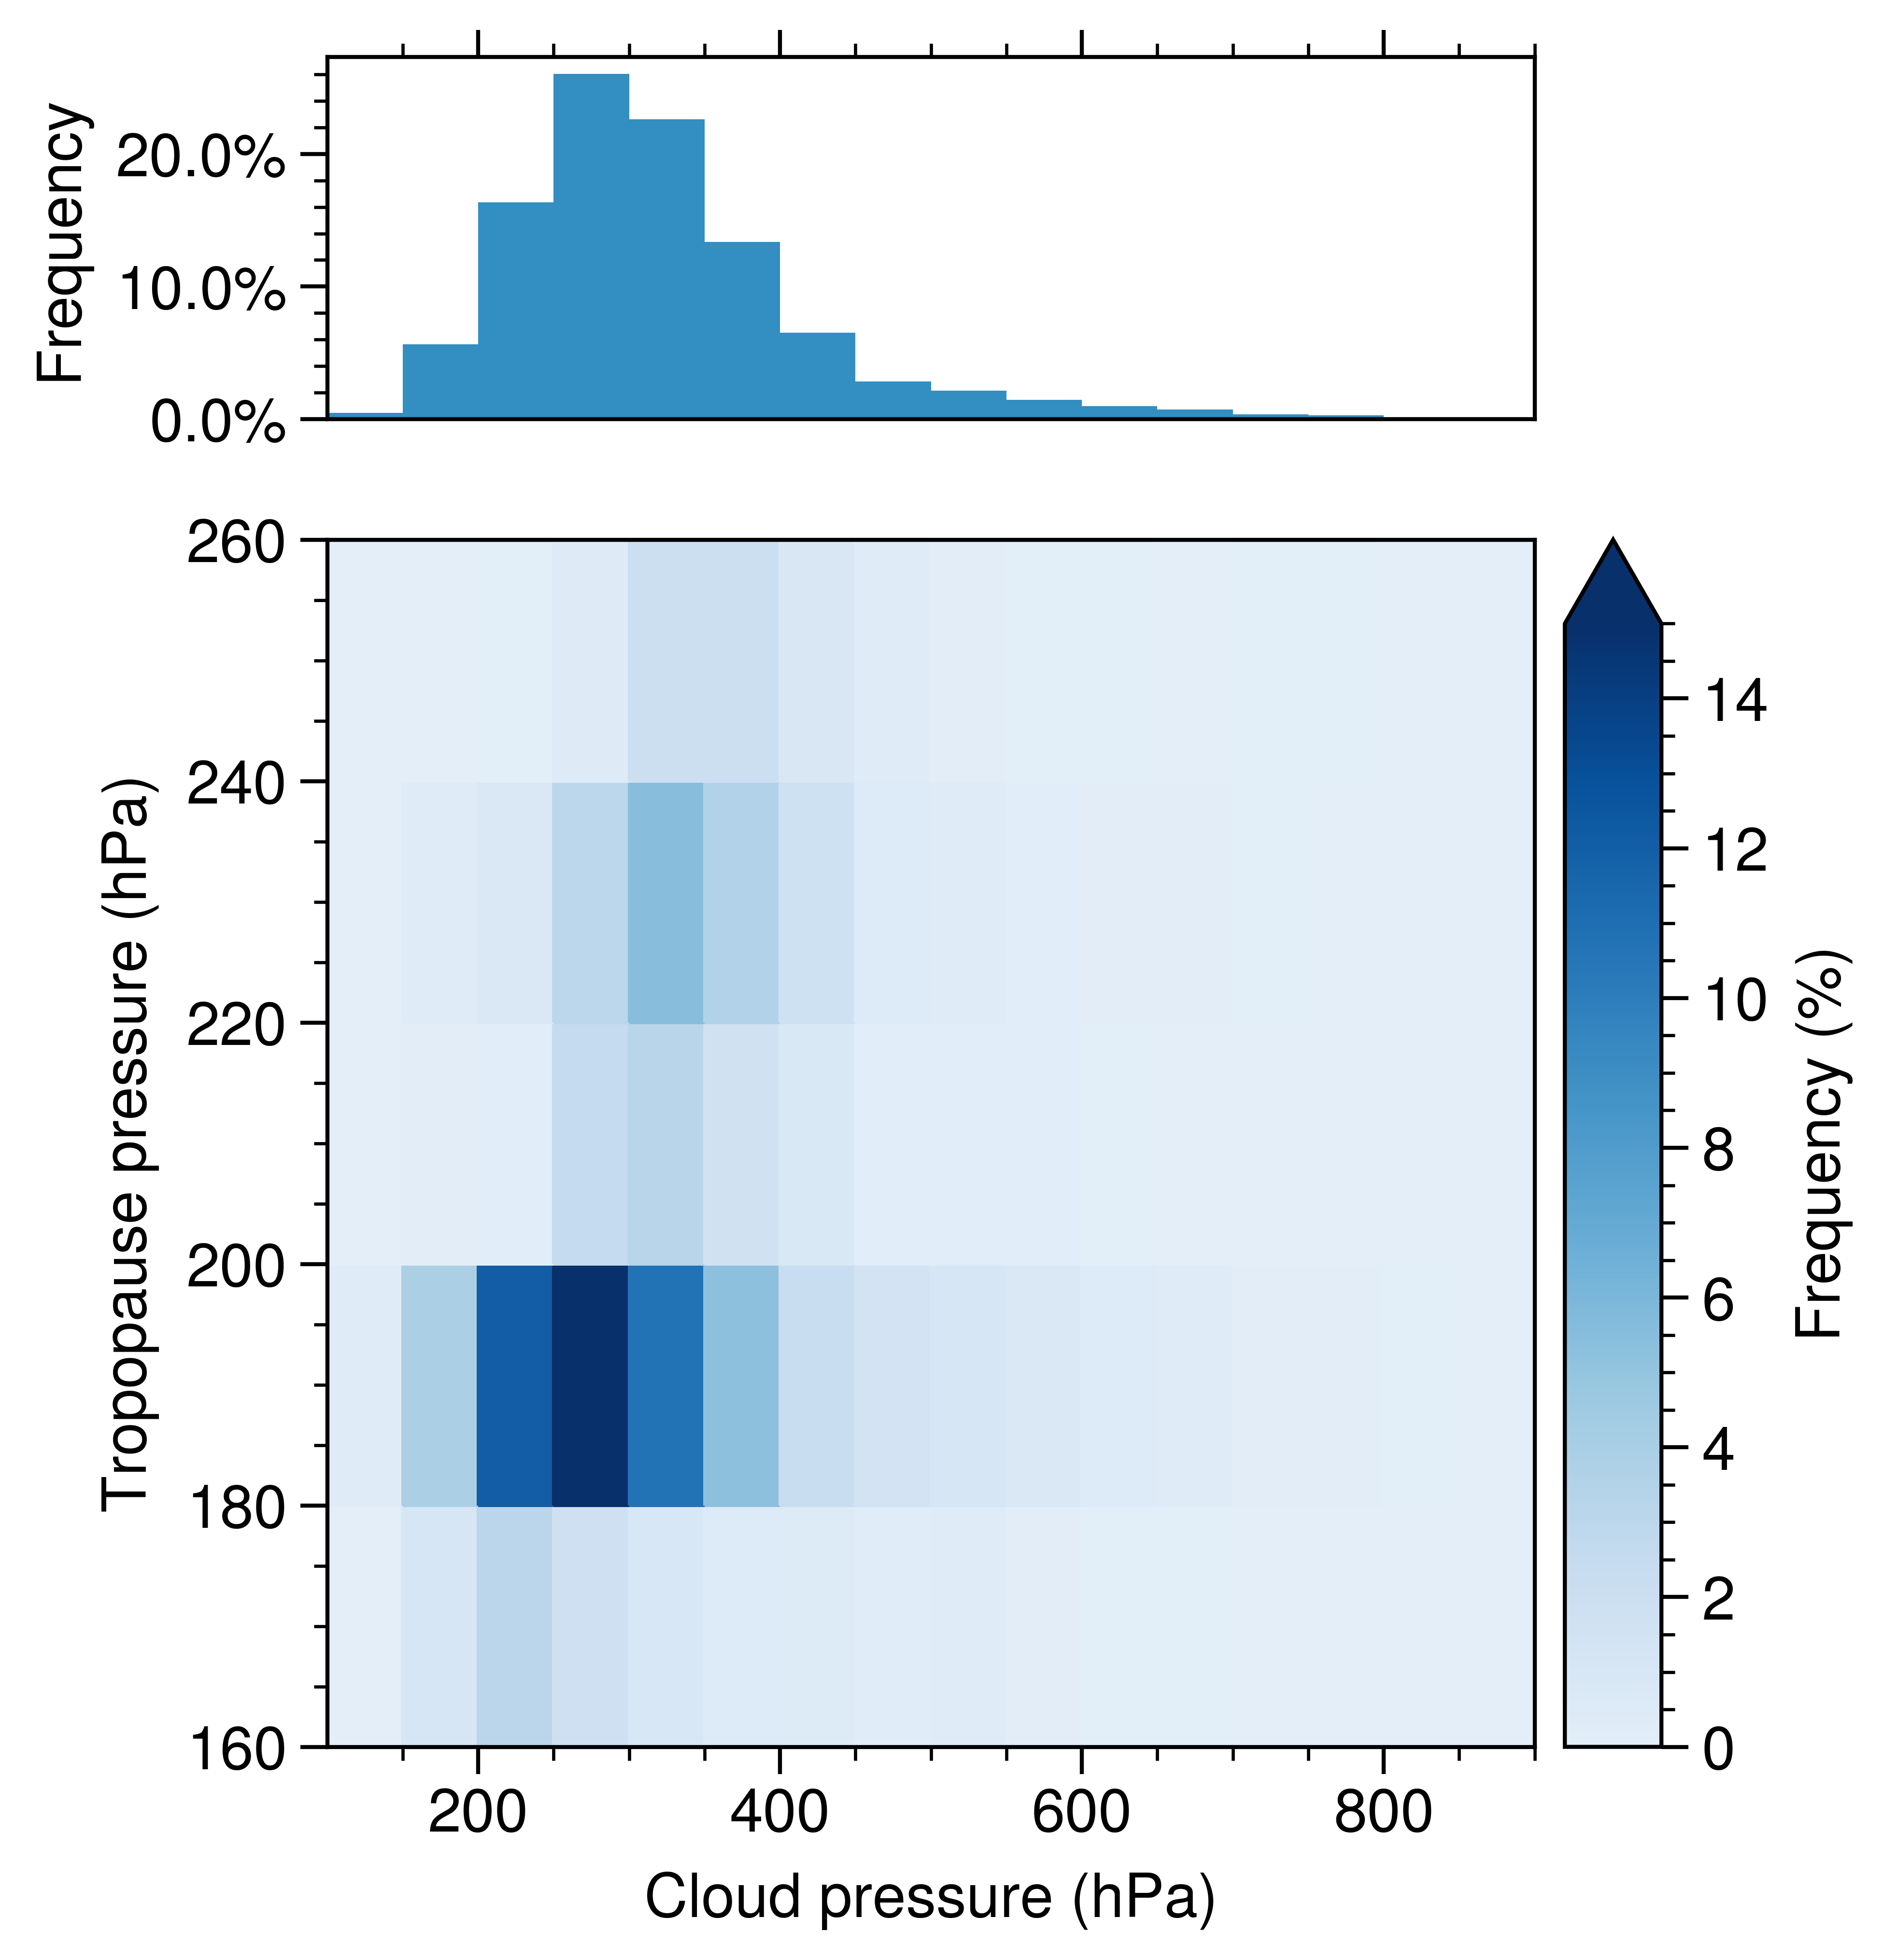
\includegraphics[width=0.6\textwidth]{./figures/pcld_ptropo.png}
\caption{云辐射分数大于0.7的像素上TROPOMI测得的云压和对流层顶高度直方图。\\
Figure \ref{fig:pcld_ptropo}. The histogram of TROPOMI cloud pressure and tropopause pressure over lightning
pixels with the cloud radiance fraction larger than 0.7.
}
\label{fig:pcld_ptropo}
\end{figure}

\subsection{云切片算法} \label{sec:cloud-slicing}

前人研究表明,云切片方法(cloud-slicing)可用于计算云内O$_3$和NO$_2$的浓度,
该方法是计算O$_3$总柱浓度的对流云微分法(CCD)的拓展\citep{Ziemke.1998,Ziemke.2001}。
简要来说,是通过线性拟合OMI或TROPOMI测得的云上NO$_2$或O$_3$柱浓度和$p_{cloud}$的斜率,从而得到NO$_2$或O$_3$的浓度,计算方法的框架见图\ref{fig:cloud-slicing_schematic}。

以TROPOMI的NO$_2$产品为例,对于不同的$p_{cloud}$我们需要至少两个邻近的云上$V_{\ch{NO2}}$($V_{\ch{NO2Vis}}$,图\ref{fig:cloud-slicing_schematic}a),这两个测量的结果显示在图\ref{fig:cloud-slicing_schematic}b 中的$p_{cloud}$-VCD 坐标平面中。
两个气压层$p_1$ 和 $p_2$($p_1$ $<$ $p_2$)之间的$V_{\ch{NO2}}$
可以通过对$p_1$--$p_2$间的NO$_2$体积混合比($VMR_{\ch{NO2}}$)进行积分得出:
\begin{equation} \label{eq:vmr_integ}
{VCD_{\ch{NO2}}}_{p_1}^{p_2}=\frac{R_{\ch{air}}}{k_Bg} \cdot \int_{p_1}^{p_2} VMR_{\ch{NO2}}(p) \mathrm{d} p
\end{equation}
其中 $R_{\ch{air}}$ 是气体常数,$k_B$ 是玻尔兹曼常数,$g$ 是重力加速度。
假设式(\ref{eq:vmr_integ})中 $p_1$ 到 $p_2$ 范围内的混合比恒定,此气压层内的平均$VMR_{\ch{NO2}}$由下式给出:
\begin{equation}
VMR_{\ch{NO2}} = \frac{\Delta V_{\ch{NO2Vis}}}{\Delta p} \frac{k_B g}{R_{air}}
\end{equation}

\begin{figure}[H]
\centering
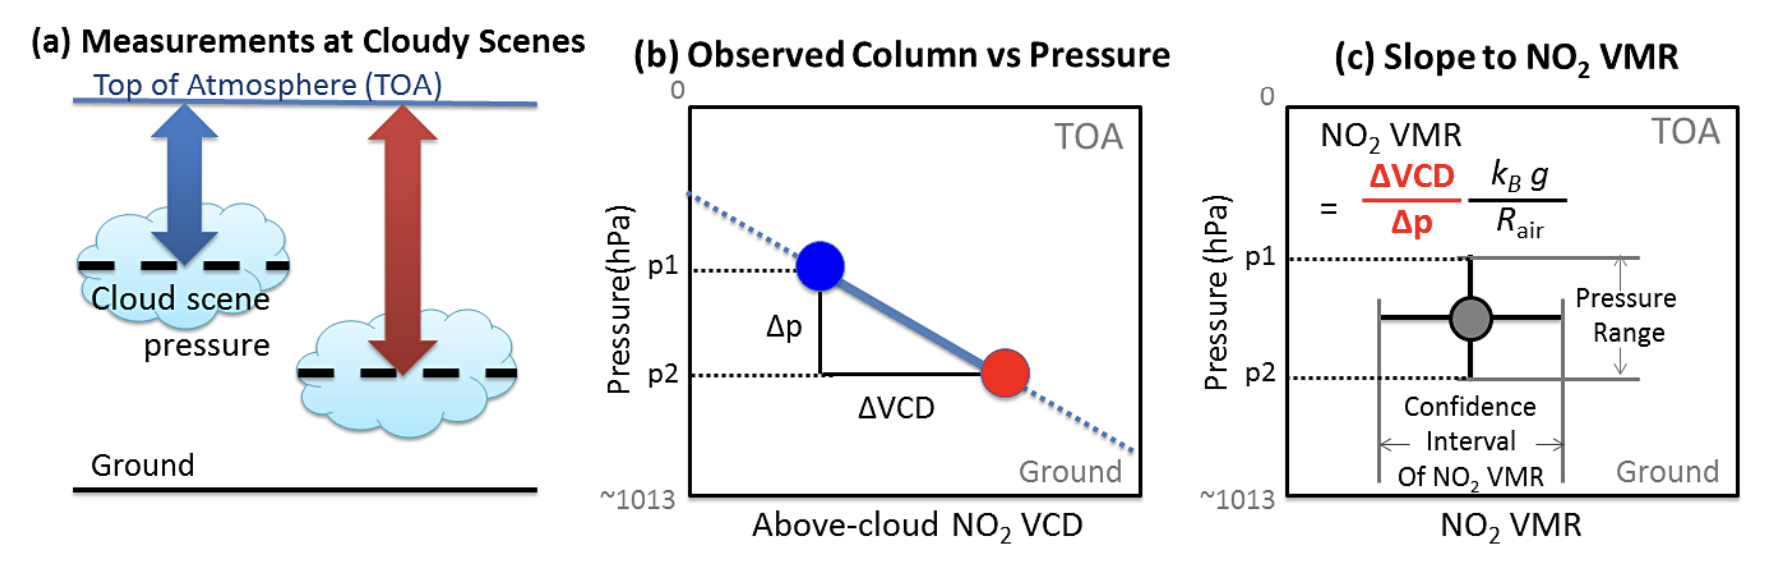
\includegraphics[width=\textwidth]{./figures/cloud-slicing_schematic.png}
\caption{云切片技术示意图(未按比例):(a)在不同云压条件下的两次云上NO$_2$ 柱浓度测量(蓝色:云压低的柱浓度;红色:云压高的柱浓度);
(b)在气压柱坐标平面上显示的测量值; (c)NO$_2$体积混合比(VMR)源自云上NO$_2$垂直柱浓度(VCD)与云压的斜率,置信区间为水平误差条和气压范围为垂直误差条。[图片来源:\citet{Choi.2014}]\\
Figure \ref{fig:cloud-slicing_schematic}. Schematic view of the cloud-slicing technique (not to scale):
(a) two above-cloud NO$_2$ column measurements at different cloud scene pressures (blue: column with lower scene pressure; and red: column with higher scene pressure);
(b) the measurements shown on a pressure-column coordinate plane;
(c) NO$_2$ volume mixing ratios (VMR) derived from the slope of above-cloud NO$_2$ vertical column densities (VCD) versus cloud scene pressure with confidence interval (horizontal error bar) and pressure range (vertical error bar). [Image source: \citet{Choi.2014}]
}
\label{fig:cloud-slicing_schematic}
\end{figure}

从这个关系式可以看出,TROPOMI云压范围内的$VMR_{\ch{NO2}}$与$V_{\ch{NO2Vis}}$和$p_{cloud}$的拟合斜率成正比(图\ref{fig:cloud-slicing_schematic}c)。
如果有两个以上的观测值,则可以从线性拟合中推导出$VMR_{\ch{NO2}}$的置信区间,
即图\ref{fig:cloud-slicing_schematic}c中$VMR_{\ch{NO2}}$的云压范围(垂直误差条)以及置信区间(水平误差条)。
在本文中,我们利用TROPOMI、TM5和MERRA2-GMI数据生成了各自在2019年6--8月对流层各高度区间内的平均$VMR_{\ch{NO2}}$,其中$p_{cloud}$位于以 330、450、570、670、770 和 870 hPa 为底的云压区间内。
由于TM5的NO$_2$为TROPOMI NO$_2$的附属产品,
故利用与下文TROPOMI相同的筛选条件进行数据筛选。
而MERRA2-GMI则选择当地时下午2点的模拟数据,计算每个云层区间内的最大云量,若某区间内的最大云量$>$ 0.4,则判断该区间为多云,并计算平均$VMR_{\ch{NO2}}$。

具体而言,$V_{\ch{NO2Vis}}$有两种计算方法:
1)基于近朗伯多云AMF假设,即具有较大总光学深度的散射云均匀分布在薄层上\citep{Choi.2014};
2)几何AMF,即$AMF_{\ch{geo}}$ = sec(SZA) + sec(VZA),其中 SZA 和 VZA 分别是太阳和视角天顶角\citep{Marais.2018,Marais.2021}。
由于对流层上层中NO$_2$垂直分布的不确定性\citep{Travis.2016},我们使用$AMF_{\ch{geo}}$来计算云切片方法需要的$V_{\ch{NO2Vis}}$。
\citet{Choi.2014}的研究表明,该计算方法得到的$V_{\ch{NO2Vis}}$在对流层中层(650 hPa)最多比近朗伯多云AMF方法计算的结果高14\%。
因此,云切片算法中的$V_{\ch{NO2Vis}}$表达式如下:
\begin{equation}
\begin{split}
V_{\ch{NO2Vis}} & = \frac{S_{\ch{NO2}}}{AMF_{\ch{geo}}} \\
             & = \frac{S_{\ch{total}}-(V_{\ch{strat}} \cdot AMF_{\ch{strat}})}{\sec (\mathrm{SZA})+\sec (\mathrm{VZA})}
\end{split}
\end{equation}
其中$S_{\ch{total}}$是总NO$_2$斜柱浓度,$V_{\ch{strat}}$为平流层NO$_2$垂直柱浓度,$AMF_{\ch{strat}}$为平流层空气质量分子。


虽然云切片方法无需知道具体的平流层NO$_2$柱浓度即可推导出对流层的$VMR_{\ch{NO2}}$,但它依赖于以下假设和条件:
1)仅适用于有相对大量的多云像素处于邻近位置,且这些像素具有足够的云压变化;
2)NO$_2$在给定的云压和空间范围内,需在垂直和水平方向上充分混合;
3)平流层柱浓度在像素区域内保持不变;
4)计算得到的$VMR_{\ch{NO2}}$绝对量级仅与$V_{\ch{NO2Vis}}$具有一样的准确度,云压也可能会带来额外的不确定性。
因此,我们参考\citet{Marais.2021}设置了以下限制条件来获得有效的云切片结果。
首先将SZA $\geq$ 80$^{\circ}$ 和表面反照率 $\geq$  30\%的像素数据去除。
接着提取多云的像素[云辐射分数(CRF)$>$ 0.7],以最大限度地减少来自对流层下层的污染。
然后将每日的像素分配到1$^{\circ}$ $\times$ 1$^{\circ}$的网格中,保留满足云压具有足够大的变化范围[云压距离 $>$ 0.5*(最高云的气压 - 最低云的气压),且标准差$>$ 30 hPa]和充分混合的NO$_2$(NO$_2$ 垂直梯度 < 0.33 pptv hPa$^{-1}$)的像素。
若网格中像素个数超过10,则将得到的$VMR_{\ch{NO2}}$赋值到该日的网格点,最后可得到各高度的季节平均$VMR_{\ch{NO2}}$。



\section{大气化学模式}

\subsection{WRF-Chem模式}

WRF-Chem是将WRF模式与大气化学模块结合起来的大气化学模式,
可用于模拟大气中微量气体和颗粒物,研究大气动力学和化学过程之间的相互作用。
该模式包含了大量的化学反应、气溶胶过程、辐射以及各类排放源(如电力厂、交通和工业),可以准确模拟大气中各类气体和颗粒物的行为。
WRF-Chem模式的一个关键优势是它能够在高时空分辨率下模拟大气化学过程,使研究人员可以详细研究地区和局部范围内化学物质和颗粒物。
此外,该模式可以采用在线和离线配置,使其成为一种灵活的工具,可以针对不同的研究问题和计算资源进行调整。
WRF-Chem模式的另一个优势是它与其他模式(如陆地表模式和海洋模式)兼容,使研究人员可以研究土地利用、海洋和大气的相互影响和相关的化学过程。这些模式结合可以给出一个全面的地球系统研究方案。
另外,WRF-Chem模式的数据输入和输出也很灵活,可以从大量的气象数据和大气化学数据源中获取数据,并将模拟结果输出到不同的数据格式,以方便进一步分析和研究。
总体而言,WRF-Chem具有高空间和时间分辨率、灵活性和兼容性等优势,其物理和化学方案的结合使得WRF-Chem模式具有更高的科学性和实际应用价值。

WRF-Chem的物理方案包括对大气温度、气压、风速等的模拟,同时考虑了太阳辐射、长波辐射、短波辐射等因素。
此外,WRF-Chem还考虑了多种化学反应,如光化学反应、氧化反应等。
该模式的化学方案包括大气中多种物质的模拟,如空气污染物(SO$_2$、NO$_x$等)、温室气体(CO$_2$、CH$_4$等)、气溶胶等。
WRF-Chem的化学方案主要包括MOZART(Model for Ozone and Related Chemical Tracers),
CBMZ(Carbon Bond Machanism)和RADM2(Regional Acid Deposition Model, 2nd generation)等多种方案。
本研究所使用的MOZART化学方案中,对流层化学以81种化学物种为代表,参与38种光解和159种气相反应\citep{Emmons.2010}。
MOZART机制包括非甲烷挥发性有机物(NMVOC)、乙烷、丙烷、乙烯、丙烯、甲醇、异戊二烯和$\alpha$-蒎烯,
其他NMVOC物种则基于反应性官能团表示。
由于本文为了更好的模拟出深对流系统,不同的个例使用了各自的方案,具体配置见\ref{sec:model_settings_us}节和\ref{sec:model_settings_china}节。



\subsection{MERRA2-GMI模式}

现代研究和应用回顾分析(MERRA-2)GMI 模式是基于Goddard地球观测系统(GEOS)框架\citep{Molod.2015},
使用的再分析资料为MERRA-2\citep{Gelaro.2017},化学机制为GMI(Global Modeling Initiative)的平流层和对流层化学相结合的机制\citep{Duncan.2007,Oman.2013,Nielsen.2017}。
GMI机制包括对O$_3$--NO$_x$--碳氢化合物化学的详细描述,有100多个物种和大约400个化学反应,
并使用戈达德化学气溶胶辐射和传输(GOCART)气溶胶模块。
模拟在立方球体上运行,其水平分辨率约为 50 km,并输出到原生 MERRA-2网格(0.625$^{\circ}$ $\times$ 0.5$^{\circ}$)。

该模式以回放方式运行,\citet{Orbe.2017}对此进行了详细描述。
简而言之,该模式最初以自由状态向前运行,并与 3 小时平均MERRA2 气象场(纬向和经向风、温度、气压)进行比较。
评估两者之间的差异并对模式进行倒回,在每个时间步长上加上所需的增量,将模式气象场向MERRA-2再分析调整。
MERRA2-GMI曾用于研究对流层和平流层O$_3$,可以获得准确的O$_3$昼夜循环、夏季O$_3$与温度之间的关系以及OMI观测到的对流层NO$_2$和O$_3$趋势\citep{Strode.2017,Ziemke.2017,Ziemke.2019}。

	%!TEX root = ../thesis.tex

\chapter{闪电氮氧化物的产率估算} \label{chapter:PE}

由于地表人为排放的NO$_x$需经过传输过程,才能到达自由对流层进而影响该层的O$_3$浓度,
而闪电直接在对流层中上层产生NO$_x$,该层的低温导致LNO$_x$寿命更长,
所以LNO$_x$可对该层的O$_3$浓度产生更大的影响。
然而,尽管前人针对LNO$_x$开展了一系列研究(见\ref{sec:intro_lnox}节),
由于难以原位观测或实验室重现,所以LNO$_x$的产率仍有很高的不确定性。
本章旨在通过使用卫星观测和云分辨化学模式来改进对LNO$_x$的估算。

本章余下部分按照以下方式组织:
\ref{sec:arctic}节将TROPOMI的NO$_2$观测和GLD360闪电探测数据相结合,
利用相邻过境数据计算旺盛对流的LNO$_x$产率和产量,并与其他NO$_x$排放源对比;
\ref{sec:us}节利用WRF-Chem的高分辨率模拟结果,定义筛选条件和新的AMF用于计算美国大陆旺盛对流的LNO$_x$柱浓度和产率;
\ref{sec:china}节在\ref{sec:us}节的基础上计算中国东南部消散对流的LNO$_x$柱浓度和产率,
最后是本章小结。


\section{清洁地区(北极)} \label{sec:arctic}

\subsection{闪电的分布} \label{subsect:lightning_distribution}

全球气候变暖正在引起闪电分布的变化\citep{Reeve.1999,Williams.2005a,Price.2009a}。
在过去的 30 年中,研究学者针对闪电预测提出了多种模拟方案\citep{Price.1992,Price.1997b,Allen.2002,Futyan.2007,Finney.2014,Romps.2014}。
气候模式模拟结果显示,中纬度地区的闪电将有所增加\citep{Michalon.1999,Romps.2014,Luhar.2021},
而在热带地区不同方案的预测结果目前仍存在分歧\citep{Finney.2018,Romps.2019}。
此外,虽然北极地区变暖速度是全球平均水平的4倍\citep{Rantanen.2022},但针对北极闪电的研究还很少。
最近,\citet{Chen.2021a}针对北极地区开发了闪电参数化方案,
结果表明:若本世纪末全球平均气温上升3.7$^{\circ}$C,永冻区的闪电频率将增加74--150\%。
地基闪电观测结果显示,北极闪电相对于全球闪电的比例在2010至2020年期间增加了两倍\citep{Holzworth.2021}。
此外,北极地区在夏季将有更多的水汽辐合来加强对流系统,从而导致更多的闪电\citep{Bintanja.2020}。

为了研究北极地区的闪电变化,我们将光学瞬态探测器(OTD,1996--1999)的卫星闪电数据
与维萨拉全球地基雷电数据集(GLD360,2019--2021)进行比较。
其中OTD的数据产品为闪电次数,一次闪电可包含一个或多个闪击。
虽然GLD360官方产品只包含闪击,但是我们的目的是研究闪电分布的变化,故未将闪击聚类成闪电。
GLD360数据覆盖了整个高纬度地区($>$60$^{\circ}$ N),而OTD仪器只观测到75$^{\circ}$ N以南的闪电。
在2019--2021年夏季(6月至8月)GLD360探测到75$^{\circ}$ N 以北发生的闪击所占比例为3\%(图\ref{fig:gld360_tseries})。

\begin{figure}[H]
\centering
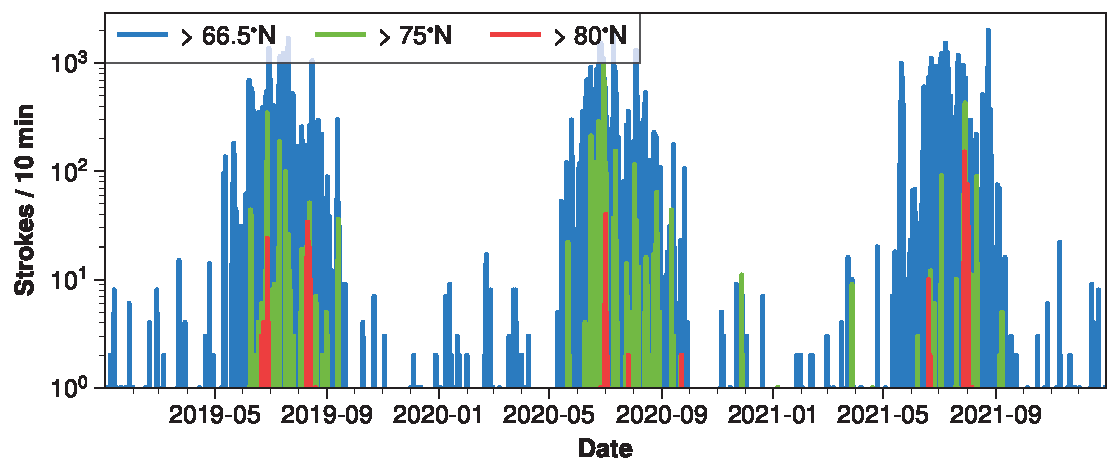
\includegraphics[width=12cm]{./figures/arctic_gld360_tseries.png}
\caption{
GLD360探测的每10分钟闪击时间序列。\\
Figure \ref{fig:gld360_tseries}. Time series of GLD360 lightning strokes per 10 minutes.
}
\label{fig:gld360_tseries}
\end{figure}


如图\ref{fig:arctic_lightning_distribution}所示,我们比较了卫星和地基闪电网在高纬度地区观测到的夏季闪电空间分布。
两个数据集均显示北极野火的主要发生地[西伯利亚和阿拉斯加永冻区,
\citep{McCarty.2021}]具有较高的闪电频率(图\ref{fig:arctic_lightning_distribution}a,b)。
OTD测得的平均闪电频率和GLD360测得的平均闪击频率分别为0.22 km$^{-2}$每月和0.61 km$^{-2}$每月。
然而,OTD 在楚科奇海(Chukchi Sea)附近记录的闪电较少,但在伊明格海(Irminger Sea)上空较多。
该现象与北极降水的年际变化和向极地输送的水汽有关\citep{Bintanja.2020}。

为了判断 TROPOMI 是否可以探测到 LNO$_2$,我们首先计算了每次TROPOMI过境前3 h内条带里发生的GLD360闪击数。
由于TROPOMI在北极地区每天有14条重叠条带,条带内的闪击数约占总数的 9\%(图\ref{fig:arctic_lightning_distribution}c),并且具有相同的地理分布(图\ref{fig:arctic_lightning_distribution}b)。
纬度越高,条带内闪击的占比越大(图\ref{fig:arctic_lightning_distribution}d),
从$<$ 10\%(60--70$^{\circ}$ N)增加到 10--25\%(70--80$^{\circ}$ N)和40--100\%(80--90$^{\circ}$ N)。
而地基观测\citep{Schmale.2018} 和飞机观测\citep{Jacob.2010}的NO$_2$数据有限,
因此TROPOMI的观测数据在分析北极的 LNO$_2$ 方面非常有利。
鉴于 70$^{\circ}$ N 以北具有更高的 TROPOMI 覆盖率和更少的其他NO$_2$排放源(例如野火或天然气),我们选择该区域来计算LNO$_2$ 产率。
如表\ref{table:arctic_emission})所示,GLD360在70$^{\circ}$ N 以北探测到的夏季闪击数分别为 1.2$\times$10$^6$ (2019)、1.6$\times$10$^6$ (2020) 和 9.8$\times$10$^5$ ( 2021)。
其中在TROPOMI 覆盖率最高的地区(80--90$^{\circ}$ N),2021 年的闪击数约为 2.9$\times$10$^4$,是前九年总数的近两倍\citep{networktotal.2021}。
GLD360测得的闪击最北可达89.5$^{\circ}$ N,WWLLN也探测到了该次闪击[89.6 $^{\circ}$ N,\citet{Holzworth.2021}]。


\begin{figure}[H]
\centering
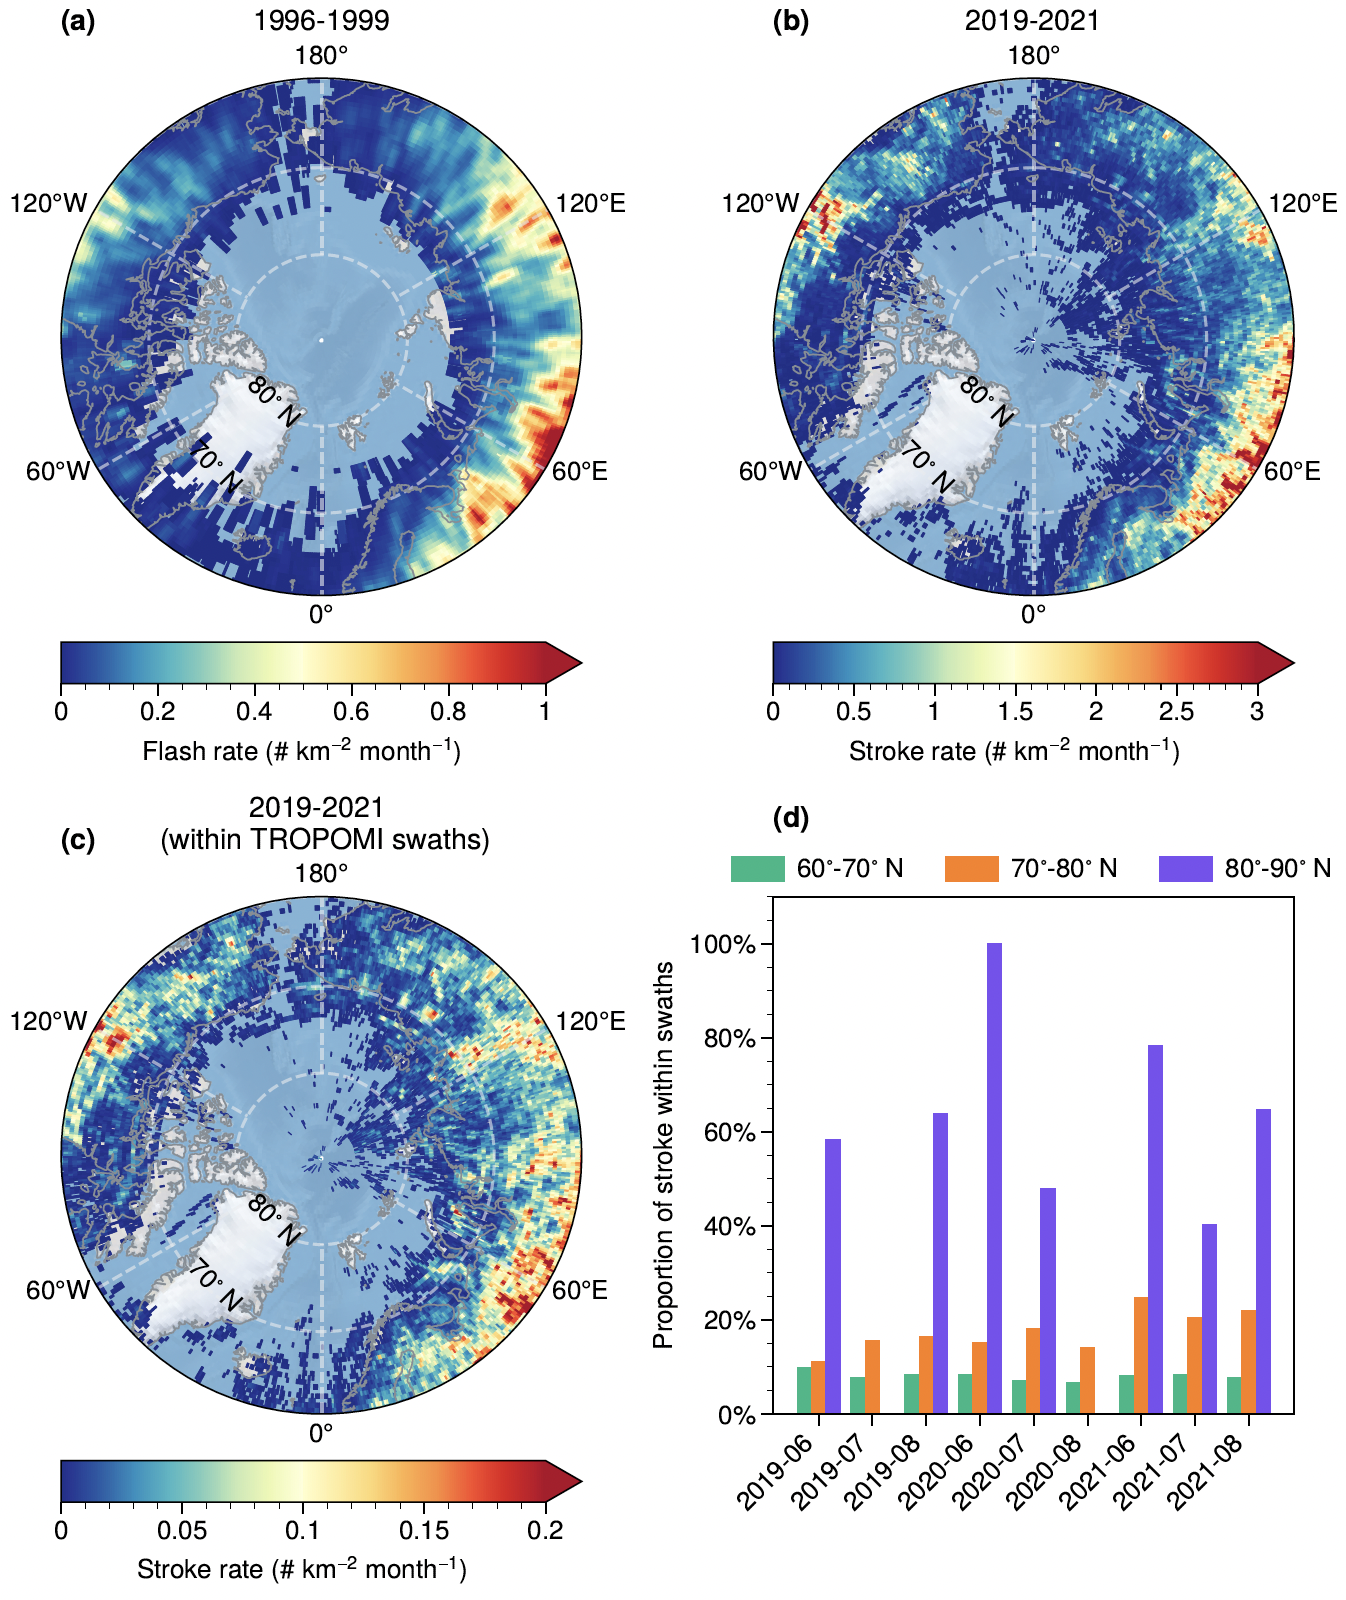
\includegraphics[width=13cm]{./figures/arctic_lightning_distribution.png}
\caption{
(a)1996至1999年6-8月OTD观测的平均闪电频率;
(b)2019至2021年6-8月GLD360观测的平均闪击频率;
(c)与(b)相同,但只计算TROPOMI过境前3 h内TROPOMI条带内的闪电;
(d)为(c)与(b)的月比例。\\
Figure \ref{fig:arctic_lightning_distribution}.
(a) Mean OTD lightning flash rate of June--August 1996--1999;
(b) Mean GLD360 lightning stroke rate of June--August 2019--2021;
(c) Same as panel b but only counting the lightning inside the TROPOMI swaths during the 3 h period before the TROPOMI overpass time.
Grids with no lightning appear as the light-blue backgrounds in panels a--c.
(d) Monthly ratio of panel c to panel b.
}
\label{fig:arctic_lightning_distribution}
\end{figure}

\begin{table*}
\centering
\caption{2019至2021年6--8月北极地区GLD360探测到的闪击数、闪电NO$_2$排放(吨氮)和平均对流有效位能(CAPE,J kg$^{-1}$)\\
Table \ref{table:arctic_emission}. GLD360 stroke counts, lightning NO$_2$ (LNO$_2$) emissions (Mg of N), and mean
convective available potential energy (CAPE, J kg$^{-1}$) in the Arctic region during June--August 2019--2021.
}
\label{table:arctic_emission}
\footnotesize
\begin{tabular}{rrrrrr}
\hline
{} & 70--75$^{\circ}$ N & 75--80$^{\circ}$ N &
80--85$^{\circ}$ N &  85--90$^{\circ}$ N &  \\
\hline
闪击 & & & & & 总数 \\
\hline
2019 &   1,142,292 &     40,660 &      5,756 &       636  & 1,189,344 \\
2020 &   1,402,304 &    233,780 &      4,784 &       768  &  1,641,636 \\
2021 &     889,248 &     62,296 &     26,576 &      2,536  &  980,656 \\
\hline
闪电NO$_2$排放 & & & & & 总数 \\
\hline
2019 &      87.3 &       5.6 &       0.9 &       0.1 &   93.9 \\
2020 &      85.5 &      22.1 &       0.8 &       0.1 &  108.5 \\
2021 &      58.6 &       8.6 &       3.9 &       0.4 &   71.5 \\
\hline
对流有效位能 & & & & & 平均值 \\
\hline
2019 & 5.5  & 4.0  & 5.0  & 6.5 & 5.3 \\
2020 & 9.2  & 5.1  & 5.0  & 5.2 & 6.1 \\
2021 & 7.3  & 4.8  & 5.5  & 7.2 & 6.2 \\
\hline
\end{tabular}
\end{table*}


\subsection{闪电氮氧化物的计算} \label{sec:arctic_lnox_calc}

LNO$_2$的估算包括以下三个主要步骤:

(1) 使用风场数据将NO$_2$柱浓度高值区与闪电数据匹配。

(2) 基于新算法来计算LNO$_2$柱浓度。

(3) 使用连续的TROPOMI观测数据来计算LNO$_2$的产率。

\subsection*{闪电的聚类}

我们使用具有噪声的基于密度的聚类方法(DBSCAN)将TROPOMI过境前12 h内\citep{Allen.2021a}的闪击以40 km进行聚类\citep{backlund2011density,Schubert.2017}。
由于野火也会产生 NO$_2$,因此使用可见光/红外成像仪/辐射计套件(VIIRS)375 m 主动火点产品,
来识别和过滤受野火排放影响的闪电聚类。
VIIRS 搭载在 Suomi 国家极地轨道合作伙伴 (Suomi-NPP)上,
它与搭载TROPOMI的S5P位于同一轨道,但比 S5P 提前3.5分钟。
我们将内部没有火点的闪电集群视为一个清洁的聚类。

对于每个清洁的闪电聚类,我们根据观测到的闪击所在位置及时间,
在三个气压层(300、500和700 hPa)上定义受 LNO$_2$ 影响的空气块(图 \ref{fig:workflow}a)。
如图 \ref{fig:workflow}b 所示,我们使用 ECMWF 小时大气再分析资料(ERA5) 的风场数据\citep{Hersbach.2020},
对含LNO$_2$ 的空气块通过水平平流进行输送,并得到TROPOMI 过境时空气块的位置。
最终的空气块组合成一个闪电掩膜(图 \ref{fig:workflow}c中的橙色圆圈),即三个等压面的前向轨迹构成了一个近似的 LNO$_2$ 区域。

我们首先使用分水岭方法得到NO$_2$垂直柱浓度($V_{\ch{NO2}}$)的高值区(图 \ref{fig:workflow}c中的像素)。
具体而言,分水岭方法将输入数据视为地形表面,并将它们分成单独的区域,称为集水盆地\citep{Soille.1990,Heikenfeld.2019a}。
在本研究中,我们应用从 4$\times$10$^{14}$ 到 1$\times$10$^{15}$ molec. cm$^{-2}$ 的阈值,步长为 2$\times$10$^{14}$ molec. cm$^{-2}$来检测多个局部NO$_2$高值特征。
这些特征用于识别具有高 $V_{\ch{NO2}}$ 的附近区域(图 \ref{fig:workflow}c 中不同颜色的像素)。
接着我们选择包含一个或多个高 $V_{\ch{NO2}}$ 区域的掩膜用于 LNO$_2$ 的进一步分析,
最终对闪电掩膜内的数据用分水岭方法进行重新识别,得到具有高 $V_{\ch{NO2}}$ 的LNO$_2$ 区域(图 \ref{fig:workflow}d 中的亮色像素)。

在重新使用分水岭方法之前,我们使用最小-最大归一化将掩膜内的 $V_{\ch{NO2}}$ 值归一化为 0 到 1 的范围,即从每个数据中减去最小值并除以最大值和最小值之间的差值。
我们将对数正态分布模型拟合到置信度为 80\% 的归一化值,并将结果用作分水岭过程的最小阈值。
由于 LNO$_2$ 区域通常小于闪电掩模(图 \ref{fig:workflow}d),
80\% 的置信水平应足以识别 LNO$_2$ 像素。
与置信度相关的不确定性见表 \ref{table:arctic_uncertainty}。
最后,我们将分水岭算法应用于标准化的 $V_{\ch{NO2}}$ 值,使用的阈值范围从最小值到 1,步长为 10,
这使我们能够识别和分析最终的LNO$_2$数据。


\begin{figure}[H]
\centering
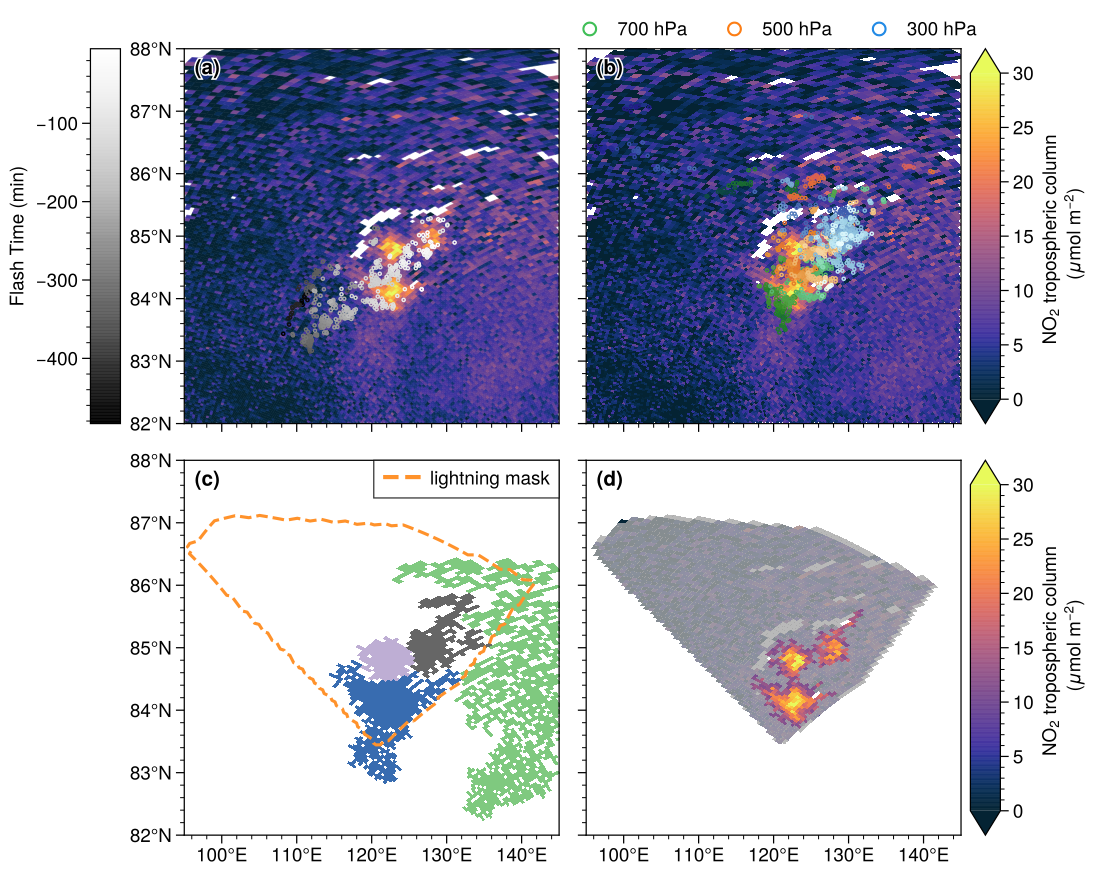
\includegraphics[width=14cm]{./figures/arctic_workflow.png}
\caption{
从 TROPOMI 轨道 09458(2019 年 8 月 1 日)数据选择闪电 NO$_2$ 像素的示意图。
背景填色为TROPOMI 检测到的 NO$_2$ 对流层柱,
(a)观测到的闪击;
(b)在三个气压层(300 hPa、500 hPa 和 700 hPa)上水平传输的闪电 NO$_2$ 空气块;
(c)将空气块组合成一个闪电掩膜(橙色圆圈),高 NO$_2$高值区(填充像素)重叠。
不同的像素颜色代表基于多个 NO$_2$ 阈值的不同 NO$_2$ 选区;
(d)掩膜内受闪电 NO$_2$ 影响的 NO$_2$ 对流层柱浓度的最终选区(亮色像素)。\\
Figure \ref{fig:workflow}. Overview of the process for identifying lightning NO$_2$ pixels from TROPOMI orbit 09458 on August 1, 2019.
The TROPOMI-detected NO$_2$ tropospheric columns are overlaid with (a) observed lightning strokes and
(b) transported air parcels of lightning NO$_2$ at three pressure levels [300 hPa (blue), 500 hPa (orange), and 700 hPa (green)].
(c) Parcels are combined into one lightning mask (orange circle), which overlaps with high NO$_2$ selections (filled pixels). The different pixel colors represent different NO$_2$ selections based on multiple NO$_2$ thresholds.
(d) Final selection (bright colored pixels) of NO$_2$ tropospheric columns affected by lightning NO$_2$ within the mask.
}
\label{fig:workflow}
\end{figure}

\subsection*{计算闪电氮氧化物柱浓度}

\citet{Zhang.2022a}指出官方 TROPOMI 算法在 NO$_2$反演中不包括 LNO$_2$,
因此我们从官方 $S_{\ch{NO2}}$产品中减去背景 NO$_2$,并将差值通过大气质量因子(AMF)转换为对流层LNO$_2$垂直柱浓度。
该算法具体为下式


\begin{equation} \label{eq:arctic_LNO2}
V_{\ch{LNO_2}} = \frac{S_{\ch{NO_2}} - S_{\ch{BG}}}{AMF_{\ch{LNO_2}}}
\end{equation}

\begin{figure}[H]
\centering
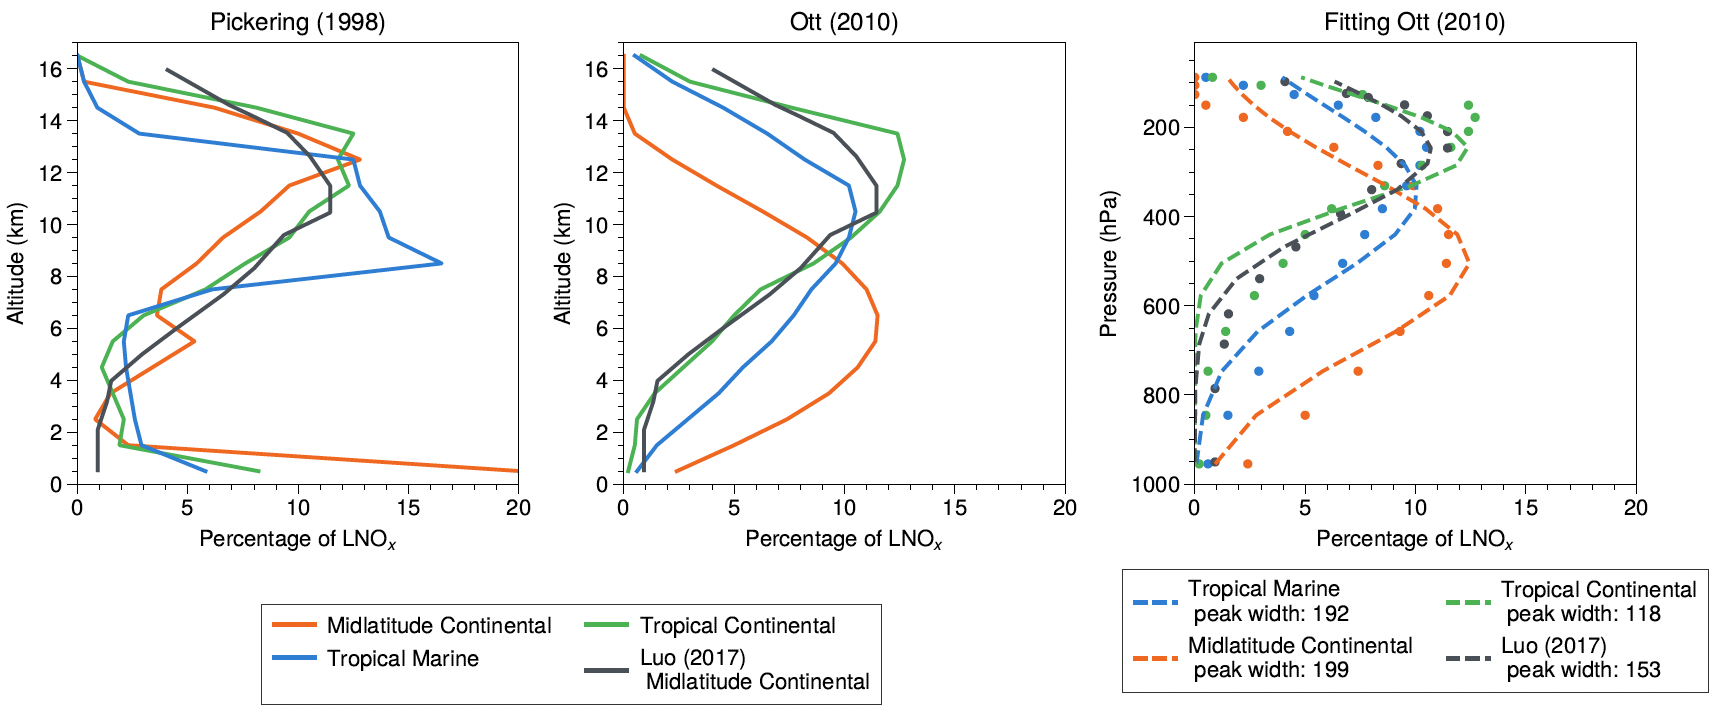
\includegraphics[width=16cm]{./figures/arctic_lnox_profile.png}
\caption{
每公里LNO$_x$质量百分比的平均垂直分布。
数据来源:(a)\  \citet{Pickering.1998};(b)\  \citet{Ott.2010},
来自\  \citet{Luo.2017} 的 LNO$_x$ 配置文件以黑色显示;
(c) 高斯拟合曲线(虚线)和原始数据(散点)。\\
Figure \ref{fig:arctic_lnox_profile}.
Average vertical distributions of percentage of typical LNO$_x$ mass per kilometer.
The LNO$_x$ profiles are from (a)\  \citet{Pickering.1998} and (b)\  \citet{Ott.2010}.
The LNO$_x$ profile from\  \citet{Luo.2017} is shown in black.
(c)  The Gaussian fitting profiles (dashed lines) and the original data (scatter points).
}
\label{fig:arctic_lnox_profile}
\end{figure}

其中 $V_{\ch{LNO2}}$ 是对流层 LNO$_2$ 垂直柱浓度,
$S_{\ch{NO2}}$ 是 TROPOMI 测得的对流层 NO$_2$ 斜柱浓度,
$AMF_{\ch{LNO2Clean}}$ 是闪电大气质量因子。
根据\citet{Allen.2021a}的研究,我们将背景 $S_{\ch{NO2}}$($S_{\ch{BG}}$)定义为对流层 AMF 和在闪电掩膜内NO$_2$低值区的第 30 个百分位数$V_{\ch{NO2}}$的乘积。
NO$_2$低值区(图 \ref{fig:workflow}d中的灰色像素)是由分水岭方法得到的$V_{\ch{NO2}}$高值区之外的所有掩膜像素。
$AMF_{\ch{LNO2Clean}}$ 是“可见”LNO$_2$ 斜柱浓度与对流层 LNO$_2$ 垂直柱浓度之比,即式(\ref{eq:AMF_LNO2clean})。
其中$LNO_2(p)$ 是与气压有关的高斯分布先验 LNO$_2$廓线,
我们将高斯分布的峰值高度设置为闪电掩模中最高的TROPOMI云压,峰值宽度设置为180 hPa。
该峰值宽度是通过高斯分布拟合前人的LNO$_x$廓线得到的,具体如下:
高斯分布由方程 $k*e^\frac{{-{(p - peak\_pressure)}^2}}{2*peak\_width^{2}}$ 给出。
在这个等式中,系数 $k$ 在 AMF 计算中同为分子和分母所以被抵消,$p$ 是TM5-MP的气压层。
利用该公式拟合 \citet{Ott.2010} 的海洋型LNO$_x$廓线和\citet{Luo.2017}的中纬度大陆型LNO$_x$廓线,
得到$peak\_width$ 的平均值为180 hPa(图\ref{fig:arctic_lnox_profile})。
我们没有使用\citet{Ott.2010}中的中纬度大陆 LNO$_x$ 廓线,是由于\citet{Luo.2017}指出该廓线与对流前的廓线相似,而本研究需要对流时的廓线。
表 \ref{table:arctic_uncertainty} 总结了与 $peak\_width$ 和云压相关的 LNO$_2$ 生产效率的不确定性。

$AMF_{\ch{LNO2}}$计算中使用的散射权重由五个参数决定:地表气压、太阳天顶角、视角天顶角、相对方位角和反照率。
对于多云部分,查找表中使用的地表气压和反照率采用云压和云反照率。
此外,我们剔除了云层高于对流层顶的个例,因为 NO$_2$ 浓度可能会受到平流层 O$_3$ 的影响\citep{Frey.2015a,Zhang.2022a}。


\subsection*{计算闪电氮氧化物产率} \label{sec:calc_lnox_pe}

如\ref{subsect:lightning_distribution}节所述,TROPOMI 可多次扫过 70$^{\circ}$ N 以北的同一点,
因此,两个连续的轨道可以观测到相同的雷暴。
为了更方便地分析北极 LNO$_2$ 案例的模式和变化,我们创建了一个网站 (\url{https://arctic-lightning-no2.streamlit.app/}),
允许用户筛选个例和以交互的方式研究LNO$_2$、云压和闪电之间的关系。

$V_{\ch{LNO2}}$(mol m$^{-2}$)在相邻过境时间之间的关系可以定义为

\begin{equation} \label{eq:relationship}
\sum_{p_{(T2)}} V_{\ch{LNO_2_i}} A_{i} = e^\frac{{-(T_2-T_1)}}{\tau} \sum_{p_{(T1)}} V_{\ch{LNO_2_j}} A_{j} + PE \sum_{N} e^\frac{{-(T_2-t_k)}}{\tau}
\end{equation}


其中 $p$ 是 LNO$_2$ 区域中的像素数,
$A$ 是每个像素的面积(m$^2$),
$T$ 是 TROPOMI 过境时间,
$t$ 是闪电发生的时间,
$\tau$ 是对流附近 LNO$_2$ 的寿命,
$PE$ 是 LNO$_2$ 的产率(mol每闪击),
$N$ 是发生在相邻过境时间内的总闪击数,
而指数成分考虑了 NO$_2$ 的化学损失。
除此之外,$i$ 和 $j$ 是 TROPOMI 的像素索引,
$A_{i}$ 和 $A_{j}$ 是不同的 LNO$_2$ 区域,并考虑了平流的影响(图\ref{fig:consecutive_orbits}),
$T_1$ 和 $T_2$ 代表 TROPOMI 在 LNO$_2$ 区域的两次平均过境时间,
$t_k$ 代表两个轨道之间发生的第 k 次雷击(k 取值范围为 1 到 N)的时间。


如果相邻过境时间内没有闪电发生,式(\ref{eq:relationship})可以简化为:

\begin{equation} \label{eq:LNO2_nolightning}
\sum_{p_{(T2)}} V_{\ch{LNO_2}_i} A_{i} = e^\frac{{-(T_2-T_1)}}{\tau} \sum_{p_{(T1)}} V_{\ch{LNO_2}_j} A_{j}
\end{equation}

我们通过分析具有高 LNO$_2$ 但两次过境时间之间没有闪电的特殊个例,得到 $\tau$ 的值为 3 $\pm$ 1 h(表\ref{table:lifetime} 和图 \ref{fig:consecutive_orbits}).
并将其代入方程(\ref{eq:relationship})来计算剩余个例的LNO$_2$产率。


\begin{figure}[H]
\centering
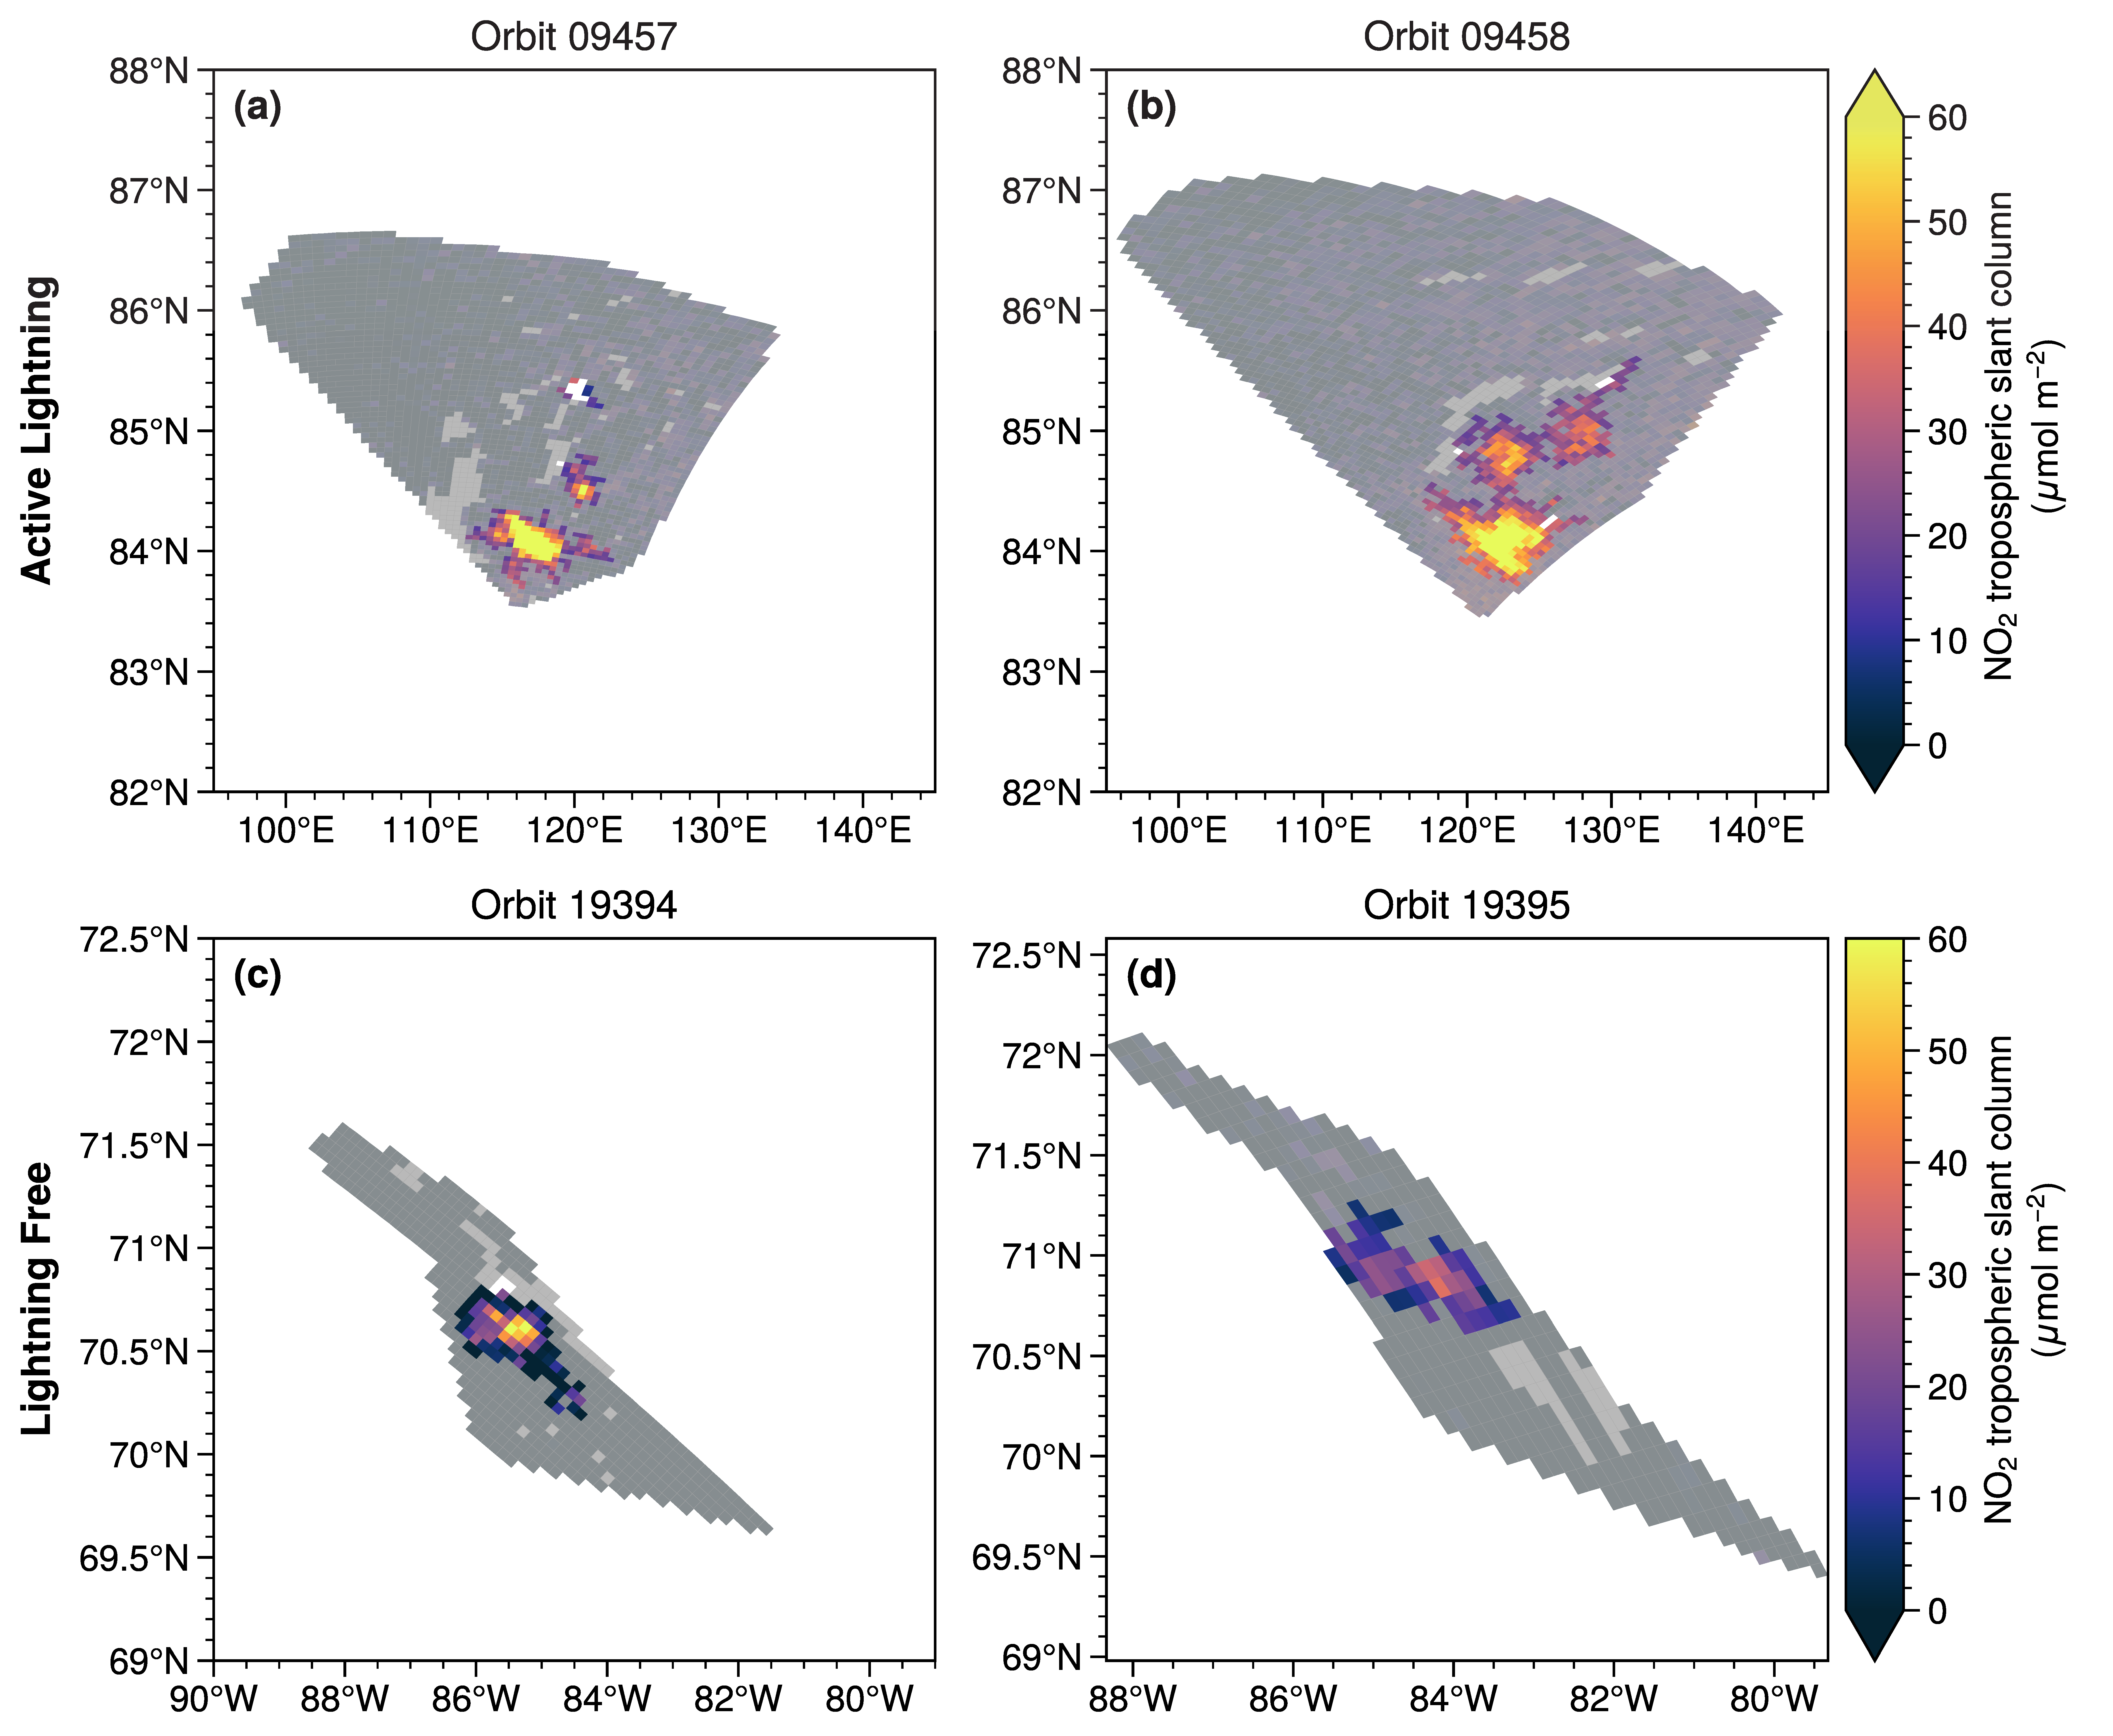
\includegraphics[width=13cm]{./figures/arctic_consecutive_orbits.png}
\caption{
受闪电 NO$_2$ 影响的 NO$_2$ 对流层柱浓度的选区(亮色像素)。
(a,b)两次连续的过境数据,且它们之间有活跃的闪电;
(c,d)两次连续的过境数据,但它们之间没有闪电。\\
Figure \ref{fig:consecutive_orbits}.
Selections (bright colored pixels) of NO$_2$ tropospheric columns affected by lightning NO$_2$.
(a--b) Two consecutive orbits with active lightning between them.
(c--d) Two consecutive orbits with no lightning between them.
}
\label{fig:consecutive_orbits}
\end{figure}


\begin{table}[H]
\centering
\caption{2019--2021期间得到的闪电 NO$_2$(LNO$_2$)寿命\\
Table \ref{table:lifetime}. Lightning NO$_2$ (LNO$_2$) lifetimes derived from cases (2019--2021).}
\label{table:lifetime}
\footnotesize
{\centering
\begin{tabular}{llllll}
\hline
时间             &         轨道 &    经度 &   纬度 &  $\Delta$面积(\%)$^a$ &  寿命(h)\\
\hline
2019-06-28 00:38 &       08833 &  127.4 &  81.0 &     -14.5 &       3.0 \\
2019-08-14 22:58 &       09513 &  126.0 &  70.4 &       2.0 &       1.7 \\
2020-06-09 19:11 &       13767 &  162.8 &  73.0 &     -43.8 &       3.6 \\
2020-06-15 22:18 &       13854 &  155.6 &  78.7 &      -4.4 &       3.4 \\
2020-07-15 21:19 &       14279 &  109.3 &  75.4 &       4.5 &       2.7 \\
2021-07-11 11:40 &       19395 &  -84.5 &  70.9 &      28.0 &       5.2 \\
\hline
\end{tabular}
\par }
\begin{tablenotes}
\footnotesize
\item $^a$$\Delta$面积 是 LNO$_2$ 面积在 $T_2$ 时刻相对于 $T_1$ 时刻的百分比变化
($T_1$ 和 $T_2$ 是连续条带的平均过境时间,$T_2$ > $T_1$)。
\item $^a$$\Delta$Area is the percentage change of the LNO$_2$ area at $T_2$ relative to $T_1$
($T_1$ and $T_2$ are the mean overpass time of consecutive swaths, $T_2$ > $T_1$).
\end{tablenotes}
\end{table}


在前人的研究中共有三种方法来估算热带和中纬度地区的 LNO$_2$ 产量:

(1) 背景NO$_2$加上LNO$_2$(LNO$_2$$^*$)与闪电之间的线性回归 \citep{Pickering.2016,Allen.2019,Lapierre.2020};

(2) 使用定义的大气质量因子直接得到NO$_2$ \citep{Beirle.2009,Zhang.2020b,Zhang.2022a};

(3) 算出LNO$_2$$^*$并减去背景 NO$_2$,其中背景 NO$_2$取自飞机观测 \citep{Pickering.2016,Perez-Invernon.2022} 或未发生闪电的对流像素处的平均NO$_2$ \citep{Bucsela.2019,Bucsela.2010,Allen.2021a}。

由于背景 NO$_2$ 随太阳天顶角而变化,线性回归法不适用于北极地区。
第二种方法需要使用闪电参数化进行详细的 LNO$_2$ 模拟,而目前闪电参数化的不确定性仍非常大\citep{Finney.2018,Romps.2019,Chen.2021a},尤其是在闪电数据集很少的北极地区 \citep{Holzworth.2021}。
因为 TROPOMI 检测到70$^{\circ}$ N 以北的非闪电对流个例有限,
所以最后一种方法需要的平均背景 NO$_2$数据集也不适用于北极地区的网格(即 1 $^{\circ}$ $\times$ 1 $^{\circ}$)。


\subsection{闪电氮氧化物的产率}

LNO$_2$ 排放是闪击数和 LNO$_2$ 产率(每次闪击产生的LNO$_2$)的乘积。
然而我们不可能直接根据来自单次过境的数据推导出 LNO$_2$ 产率,
因为 TROPOMI 检测到的 LNO$_2$ 由产生和消耗组成,所以时间维度上需要第二个过境数据。
我们提出可以利用连续轨道的 LNO$_2$ 来估算 LNO$_2$ 产率(见\ref{sec:calc_lnox_pe}节)。
基于对 LNO$_2$ 和闪击的筛选,我们共获得了43个个例,115 个 LNO$_2$ 选区。
其中,60$^{\circ}$ W 和 180$^{\circ}$ W 之间的个例由于 LNO$_2$ 不显著或没有足够的观测值而被剔除。
大多数个例位于 60$^{\circ}$ E 和 180$^{\circ}$ E 之间(图 \ref{fig:arctic_lno2_production}a)。
通过比较闪电分布(图 \ref{fig:arctic_lno2_production}a)与LNO$_2$总和的分布(图 \ref{fig:arctic_lno2_production}b),
我们发现 TROPOMI 观测到的 LNO$_2$ 远离LNO$_2$的排放源。
例如,喀拉海(Kara Sea)没有闪电发生 (77--80$^{\circ}$ N, 65--105$^{\circ}$ E),
但此处的LNO$_2$ 总共约为 5.1 $\times$ 10$^6$ mol。
这是由于对流层上层主导的东风对LNO$_2$的输送作用,从而揭示了匹配闪电和 NO$_2$的重要性。

尽管如此,LNO$_2$ 与闪击之间仍有一致的空间相关性,因此我们针对每个个例计算其 LNO$_2$ 产率。
研究结果表明,LNO$_2$ 产率在陆地、沿岸和海洋处为 2.0(第 25 至第 75 个百分位数:1.3--3.1)mol每闪击、
3.5(第 25 至第 75 个百分位数:1.1--13.0)mol每闪击
和11.5(第 25 至第 75 个百分位数:1.3--29.9)mol每闪击(图 \ref{fig:arctic_pe_rate}a)。
除了这些中值外,我们还得到了排名前10的LNO$_2$产率,其范围为每次闪击产生27--612 mol(表\ref{table:arctic_pe_lno2})。
这些最高值都出现在海洋或沿海地区。
由于个例数量有限,我们无法确定海洋和陆地之间的 LNO$_2$产率是否存在统计学上的显著差异。
在热带和中纬度地区的研究也表明,由于海洋上的闪电能量更高\citep{Beirle.2014,Hutchins.2013},
海洋上的 LNO$_2$产率是陆地上的两倍\citep{Marais.2018,Allen.2019,Bucsela.2019}。

最近的研究表明,LNO$_2$产率与闪电尺寸有关,尺寸越大,产生的LNO$_2$越多 \citep{Huntrieser.2008,Marais.2018}。
此外,更强的上升气流与更小的闪电和更高的闪电频率相关\citep{Bruning.2013,Bruning.2015,Mecikalski.2015}。
因此,我们计算了闪击率,即单位时间单位LNO$_2$面积内的闪击次数,
它的范围从 2.3$\times$10$^{-10} $m$^{-2}$ h$^{-1}$ 到 4.1$\times$10$^{-6} $m$^{-2 }$ h$^{-1}$,
陆地地区闪击率(6.2$\times$10$^{-7}$ m$^{-2}$ h$^{-1}$)比海洋地区高$\sim$ 11 倍(5.2$\times$10$^{-8}$ m$^{-2}$ h$^{-1}$)。
我们发现闪击率和 LNO$_2$产率之间存在近似的幂律关系(图\ref{fig:arctic_pe_rate}b)。
当闪击率下降2个数量级时,LNO$_2$产率增加10倍,这与中纬度开展的研究一致\citep{Bucsela.2019,Zhang.2020b}。


\begin{figure}[H]
\centering
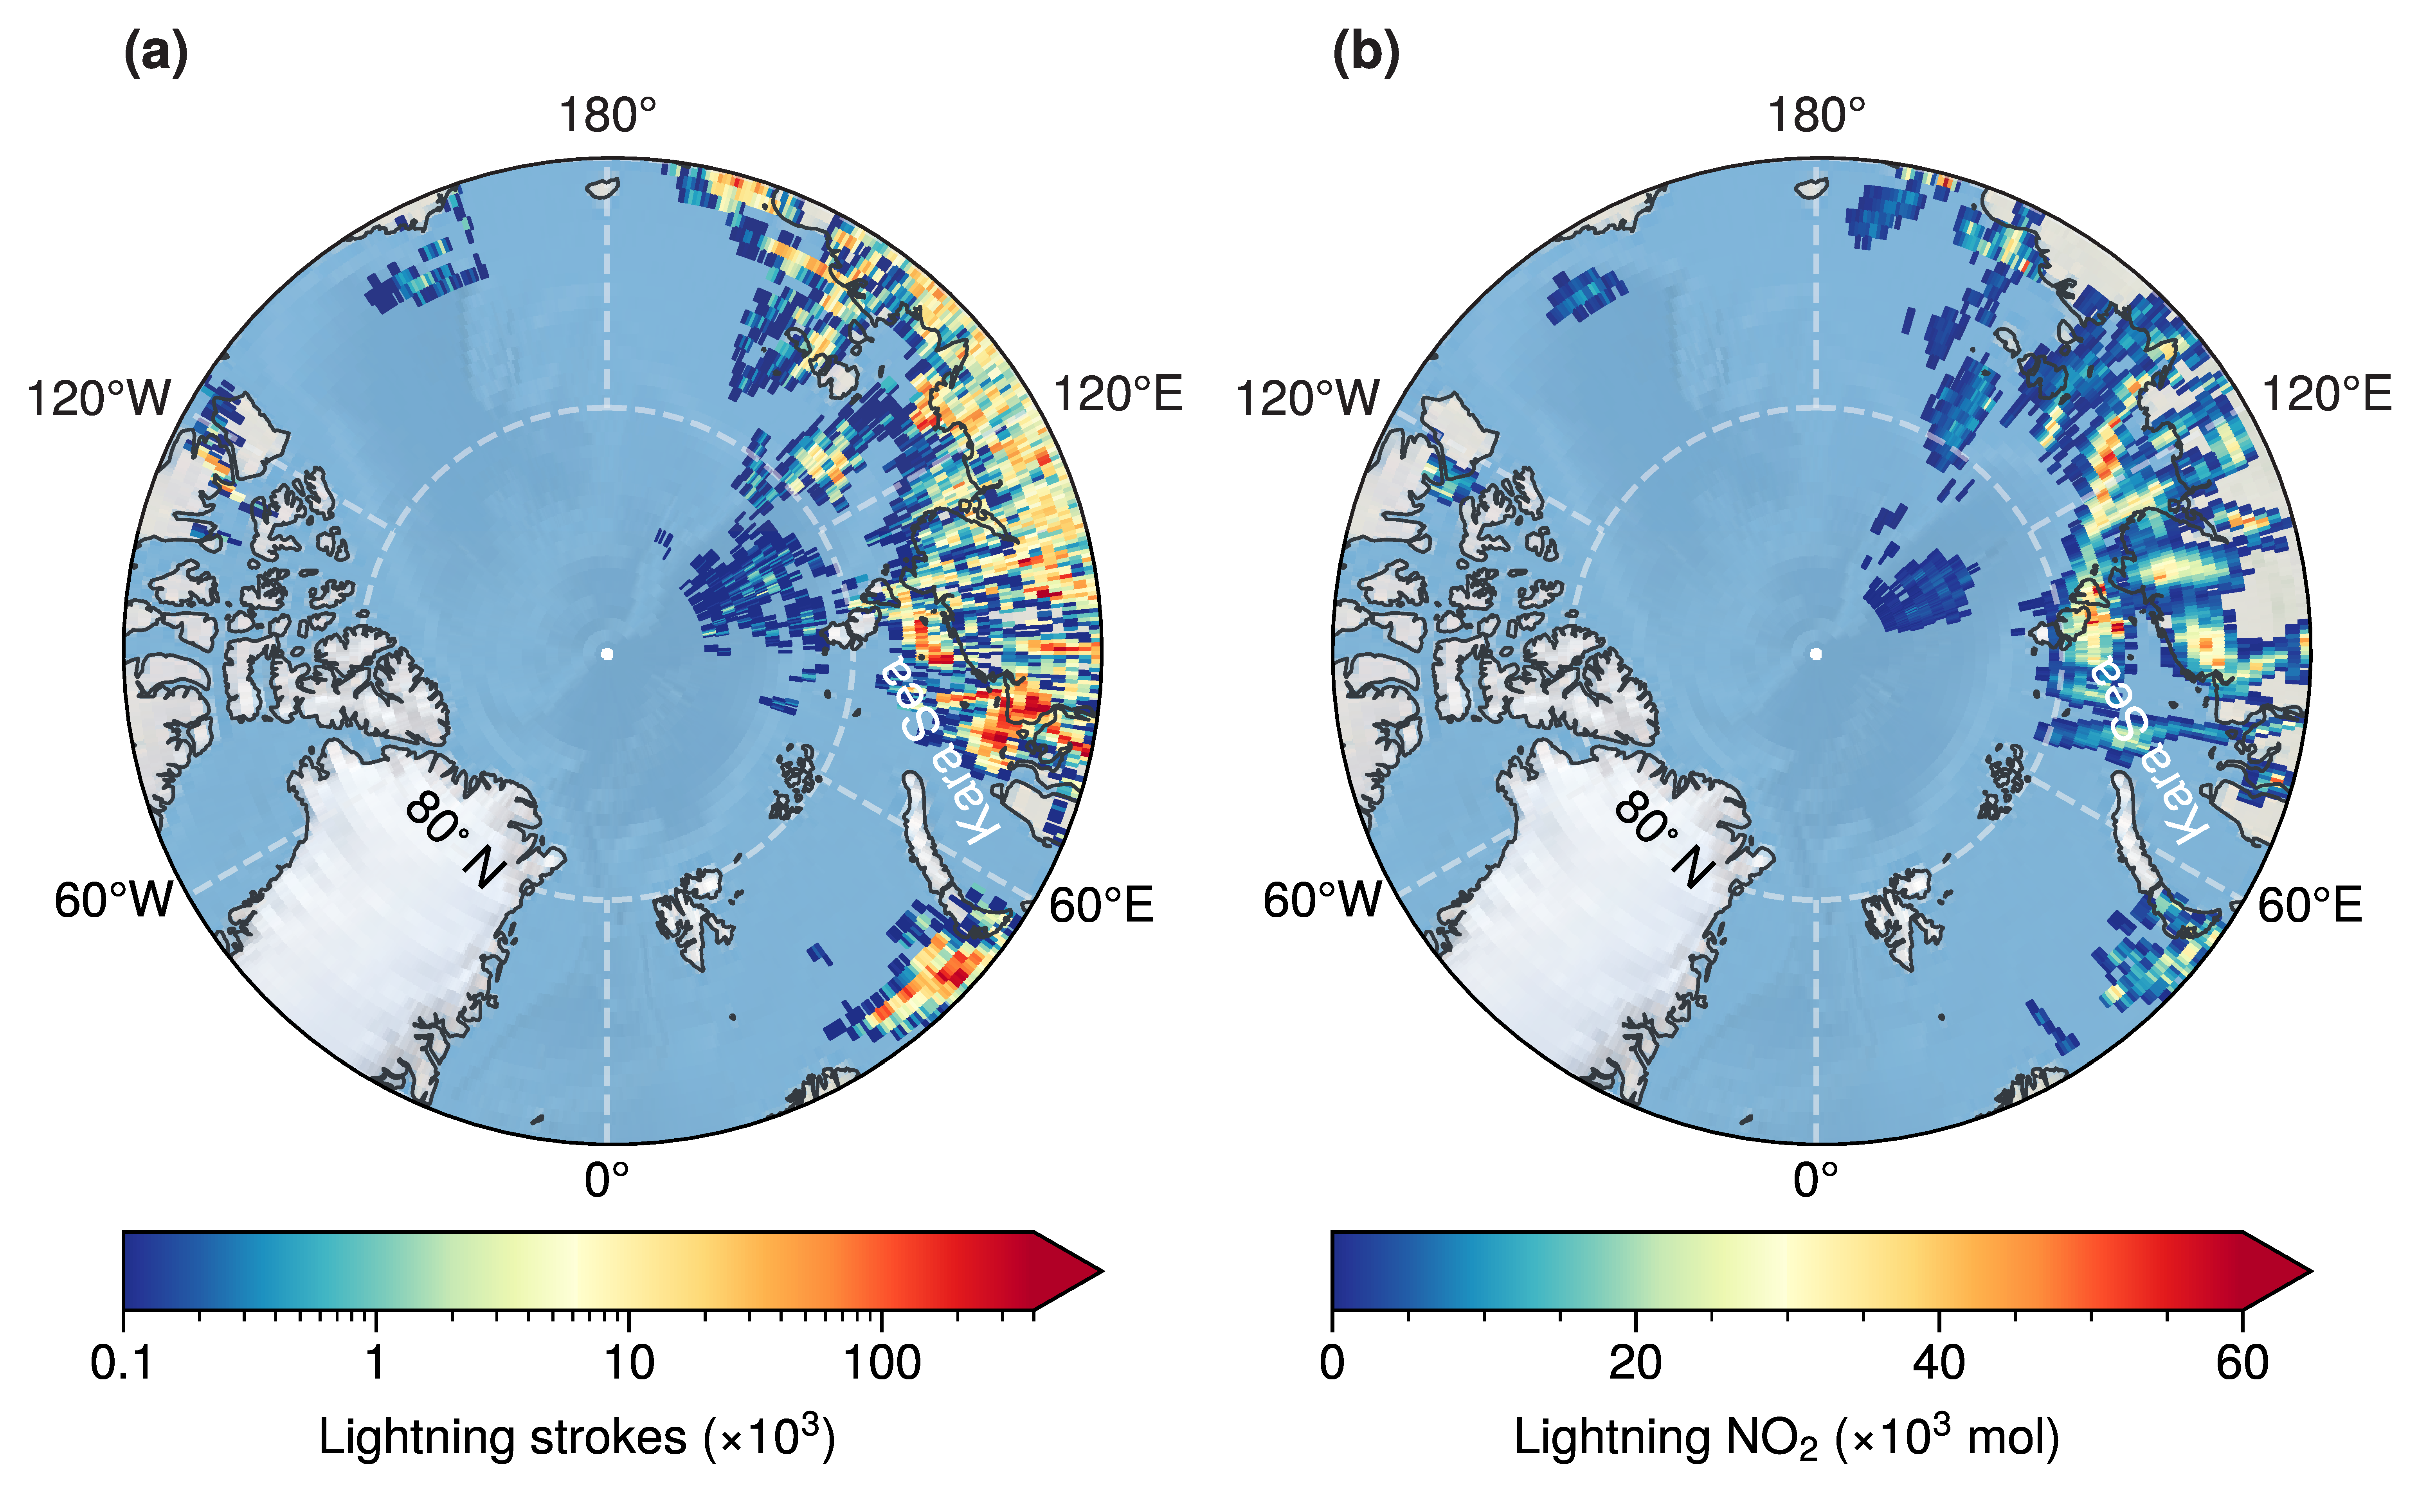
\includegraphics[width=13cm]{./figures/arctic_lno2_production.png}
\caption{
(a)每 0.5$^{\circ}$ $\times$ 0.5$^{\circ}$ 网格中所选个例的 GLD360 闪击总和;
(b)每 0.5$^{\circ}$ $\times$ 0.5$^{\circ}$ 网格中由TROPOMI观测数据所得的个例LNO$_2$ 总和。\\
Figure \ref{fig:arctic_lno2_production}. (a) Sum of GLD360 lightning strokes for selected cases per 0.5$^{\circ}$ $\times$ 0.5$^{\circ}$ grid.
(b) Sum of lightning NO$_2$ derived from TROPOMI observations for selected cases per 0.5$^{\circ}$ $\times$ 0.5$^{\circ}$ grid.
}
\label{fig:arctic_lno2_production}
\end{figure}

\begin{table}[H]
\centering
\caption{2019--2021 年10 大LNO$_2$产率 \\
Table \ref{table:arctic_pe_lno2}.
Top 10 lightning NO$_2$ (LNO$_2$) production efficiencies from 2019 to 2021.}
\label{table:arctic_pe_lno2}
\footnotesize
{\centering
\begin{tabular}{llllllll}
\hline
时间 &       条带 &   经度 &   纬度 &
区域$^a$ &
闪击数$^b$  & \shortstack{LNO$_2$ 产率 \\ (mol每闪击)} \\
\hline
2020-06-15 20:38 &  13853 &      152.7 &      78.1 &       海洋 &         124 &    611.9 \\
2019-08-11 01:54 &  09458 &      123.5 &      84.5 &       海洋 &         404 &    180.6 \\
2020-07-07 01:51 &  14154 &       53.2 &      72.8 &       沿岸 &        1676 &    151.2 \\
2019-06-26 21:37 &  08817 &      115.4 &      75.7 &       海洋 &        2516 &    144.6 \\
2019-06-20 18:29 &  08730 &      122.2 &      72.8 &       沿岸 &         436 &    105.0 \\
2019-06-20 20:09 &  08731 &      122.1 &      73.1 &       沿岸 &         396 &     81.1 \\
2019-08-11 00:13 &  09457 &      118.0 &      84.2 &       海洋 &        1068 &     51.1 \\
2019-07-11 21:51 &  09030 &      172.4 &      72.2 &       海洋 &         992 &     42.9 \\
2021-07-12 19:44 &  19414 &     -147.6 &      72.7 &       海洋 &        1512 &     32.8 \\
2020-06-16 05:02 &  13858 &      121.3 &      75.8 &       海洋 &         536 &     26.9 \\
\hline
\end{tabular}
\par }
\begin{tablenotes}
\footnotesize
\item $^a$ 陆地和海洋由50 m Natural Earth数据分类,其中沿岸地区定义为海岸线周围500 m半径。
\item $^b$ 连续轨道间隔期间的总闪击数。
\item $^a$ The land and ocean are classified by the 50 m Natural Earth data, where the coastal region is defined as a 500 m radius around the coastline.
\item $^b$ The total number of strokes during the interval between consecutive orbits.
\end{tablenotes}
\end{table}


\begin{figure}[H]
\centering
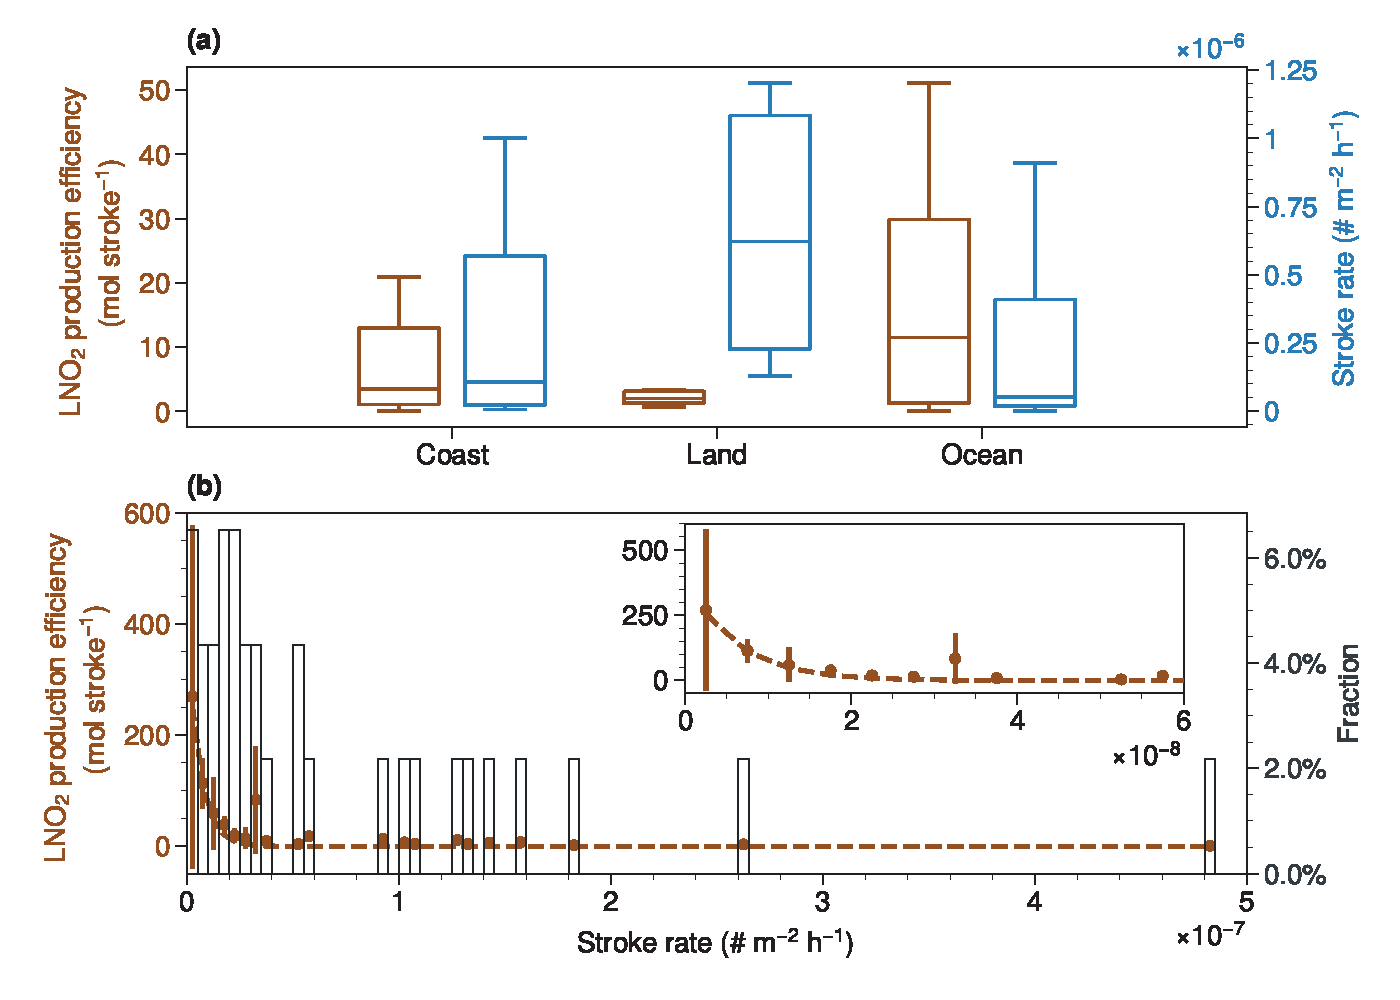
\includegraphics[width=15cm]{./figures/arctic_pe_rate.png}
\caption{
(a)三个区域(沿岸、陆地和海洋)的LNO$_2$产率(棕色)和闪击频率(蓝色),
其中沿岸地区为海岸线周围 500 m 的半径。
海岸区域定义为海岸线周围 500 m 半径范围内。
箱线图表示中值,下边界和上边界分别代表第 25 个和第 75 个百分位数,上下误差线分别代表第 10 个和第 90 个百分位数。
(b)LNO$_2$ 产率与闪击频率的关系,叠加每个 5$\times$10$^{-9}$ m$^{-2}$ h$^{-1}$ 中个例占比的直方图。 \\
Figure \ref{fig:arctic_pe_rate}. (a) Comparison of lightning NO$_2$ (LNO$_2$) production efficiency (brown) and stroke rate (blue) for three regions: coast, land, and ocean.
The coast region is defined as a 500 m radius around the coastline.
The box plots indicate the median values; the lower and upper boundaries represent the 25th and 75th percentiles, respectively, and the lower and upper error lines are the 10th and 90th percentiles, respectively.
(b) LNO$_2$ production efficiency vs stroke rate, with histograms of case fractions in each 5$\times$10$^{-9}$ m$^{-2}$ h$^{-1}$ stroke rate bin overlaid.
}
\label{fig:arctic_pe_rate}
\end{figure}


\begin{table}[H]
\centering
\caption{LNO$_2$产率估算的不确定性$^a$\\
Table \ref{table:arctic_uncertainty}. Uncertainties$^a$ for the estimation of LNO$_2$ production efficiency (PE).}
\label{table:arctic_uncertainty}
\footnotesize
\begin{tabular}{llll}
\hline
类型                           &  默认值        & 扰动                 &   不确定度 (\%)  \\
\hline
LNO$_2$ 寿命                   & 3 小时                 & 2 小时和4 小时$^b$      &   36                      \\
IC:CG                         & 1:1                    & 2:1和1:2                  &   33 \\
LNO$_2$ 廓线宽度                & 180 hPa               & 160 hPa 和 200 hPa          &   7   \\
对流层 NO$_2$ 对流层背景浓度      & 第 30 个百分位数        & 第 10 个百分位数$^c$     & 2                \\
LNO$_2$ 选区              & 80\% 置信区间          &  70\% 置信区间   & 13                \\
云压                 & 二级产品               &  $\pm$ 50 hPa$^d$                & 7                \\
其他$^e$       & --                  & --                           &   10                      \\
Net                            &                     &                              &   53                      \\
\hline
\end{tabular}
\begin{tablenotes}
\footnotesize
\item $^a$ 不确定度 = (误差$_{\ch{高扰动值}}$ - 误差$_{\ch{低扰动值}}$)/2
其中 误差$_{\ch{扰动}}$ = (PE$_{\ch{扰动}}$ - PE$_{\ch{默认值}}$)/PE$_{\ch{默认值}}$;
\item $^b$ 基于本研究得到的寿命范围。
\item $^a$ Uncertainty = (Error$_{rising\ perturbed\ value}$ - Error$_{lowering\ perturbed\ value}$)/2
where Error$_{\* perturbed\ value}$ = (PE$_{\* perturbed\ value}$ - PE$_{default\ value}$)/PE$_{default\ value}$.
\item $^b$ Based on the lifetime values calculated in this study.
\item $^c$ \ \citet{Allen.2021a} and \ \citet{Perez-Invernon.2022}.
\item $^d$ \ \citet{VanGeffen.2022}.
\item $^e$ \ \citet{Allen.2021a}.
\end{tablenotes}
\end{table}


\subsection{氮氧化物的不同排放源贡献}


图 \ref{fig:arctic_no2_comp}a 为2019--2021 年 6 月至 8 月 TROPOMI 在北极观测到的平均 NO$_2$ 柱浓度分布图,
虽然从背景中无法看出LNO$_2$,但在城市、工业和野火地区仍然可以观察到 NO$_2$ 的增强。
例如可以清楚地观察到与阿拉斯加、挪威和俄罗斯的采矿作业相关的 NO$_2$ 柱浓度高值(17 $\pm$ 2 $\mu$mol m$^{-2}$)。
石油和天然气活动也显现出明显的NO$_2$高值,
如加拿大北极麦肯齐谷、北阿拉斯加普拉德霍湾/库帕鲁克和俄罗斯亚马尔天然气管道/乌连戈气田\citep{VanDerA.2020}。
而格陵兰海岸沿线的 NO$_2$ 高值可能是与复杂地形反演相关的错误信号\citep{Hachmeister.2022}。
与 NO$_2$ 污染相反,70$^{\circ}$ N 以北的 TROPOMI 观测显示背景 NO$_2$浓度较低(4.35 $\pm$ 1.26 $\mu$mol m$^{-2}$),
比 60$^{\circ}$ N 和 65$^{\circ}$ N 之间的平均 NO$_2$ 低45\%。

通过将每个个例中LNO$_2$柱浓度的最大值(61 $\pm$ 50 $\mu$mol m$^{-2}$)与北极地区典型的人为和野火 NO$_2$ 进行比较,
我们发现 LNO$_2$ 的柱浓度为其他源的3倍,尽管排放的时间尺度是小时数量级(图 \ref{fig:arctic_no2_comp}b)。
其中发生在拉普捷夫海(Laptev Sea)上空的深对流(图\ref{fig:arctic_large_lno2}),
其LNO$_2$最大值 为 246 $\mu$mol m$^{-2}$,
与美国夏季最高 NO$_2$ 柱浓度相当[234 $\mu$mol m$^{-2}$,\citet{Goldberg.2021a}]。
考虑到LNO$_2$在短时间内的巨大贡献,因此计算北极地区LNO$_2$排放显得十分重要。

\begin{figure}[H]
\centering
\includegraphics[width=13cm]{./figures/arctic_no2_comp.png}
\caption{
(a)2019至2021年6--8月当地下午时TROPOMI测的的对流层 NO$_2$ 平均柱浓度(4 km $\times$ 4 km);
(b)四种NO$_2$来源的柱浓度比较:闪电、采矿、石油天然气和野火。
其中闪电NO$_2$浓度为每次对流个例的所有像素上NO$_2$的最大值,
而野火、采矿和石油天然气的浓度是(a)中典型位置的每日NO$_2$最大值。
框内的黑线和红线分别是中值和平均值,
下边界和上边界分别是第 25 和第 75 个百分位数,
上下误差线分别是第 10 和第 90 个百分位数。\\
Figure \ref{fig:arctic_no2_comp}(a)Mean 4 km $\times$ 4 km TROPOMI tropospheric NO$_2$ column density in the local afternoon during June--August 2019--2021.
The mining and oil and gas stations are shown as gray and red circles, respectively.
(b) Comparisons of NO$_2$ among four sources: lightning, mining, oil and gas, and wildfire.
The lightning bar represents the maximum NO$_2$ values over pixels for each lightning case,
while the wildfire, mining, and oil and gas bars are the daily maximum NO$_2$ values at typical locations.
The box plots indicate the median (black line) and mean (red line) values; the lower and upper boundaries represent the 25th and 75th percentiles, respectively, and the lower and upper error lines are the 10th and 90th percentiles, respectively.
}
\label{fig:arctic_no2_comp}
\end{figure}

\begin{figure}[H]
\centering
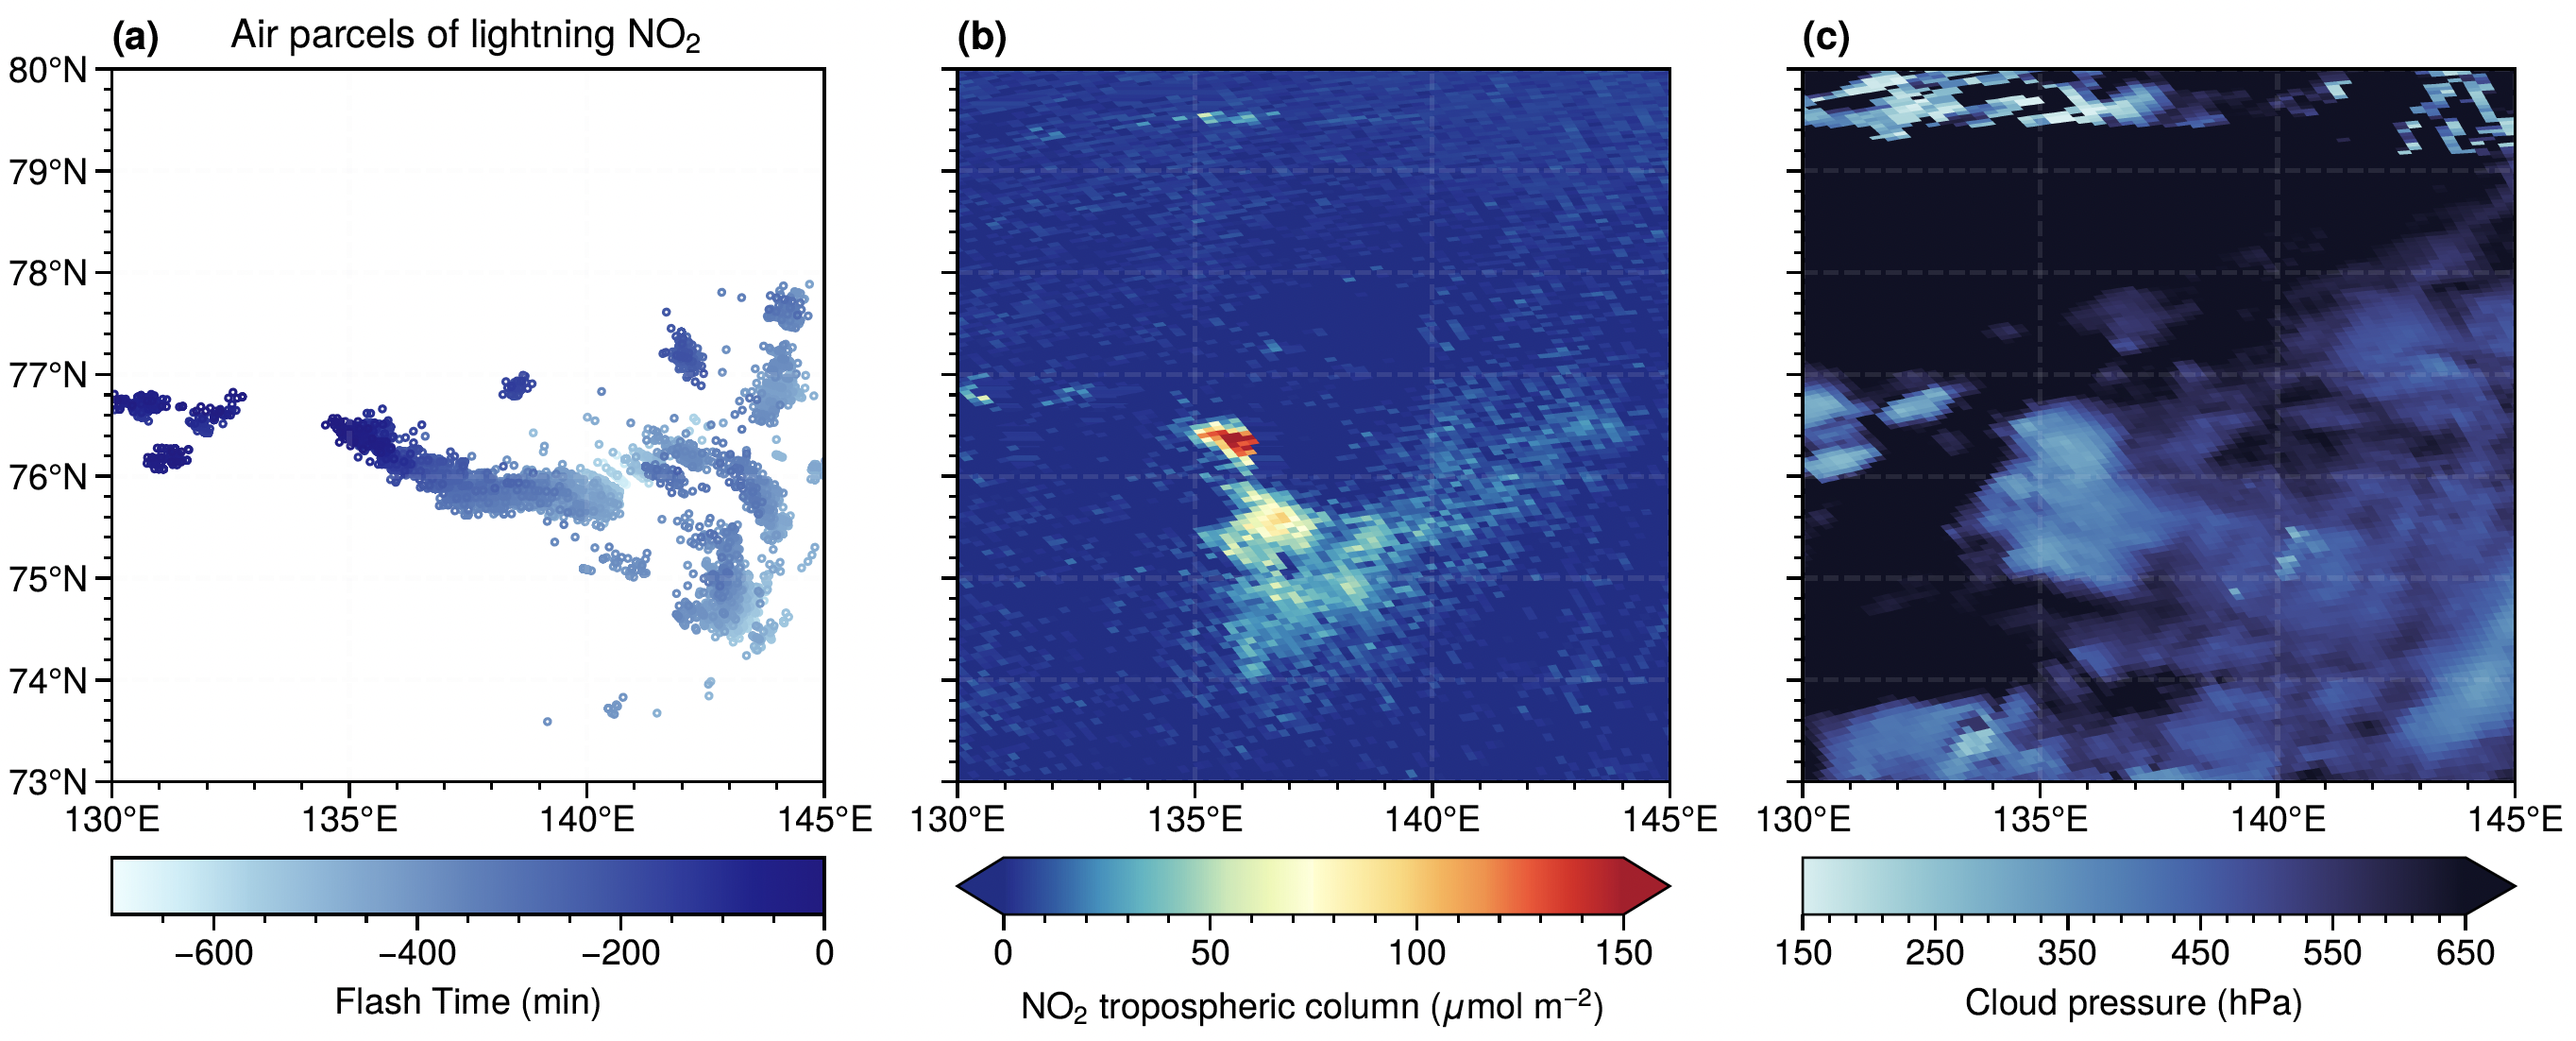
\includegraphics[width=15cm]{./figures/arctic_large_lno2.png}
\caption{
(a)在 500 hPa气压层水平传输的包含闪电 NO$_2$ 的空气块;
(b)TROPOMI 观测到的 NO$_2$ 对流层柱浓度;
(c)TROPOMI 观测到的云压。\\
Figure \ref{fig:arctic_large_lno2}. (a) Transported air parcels containing lightning NO$_2$ at 500 hPa pressure level.
(b) The TROPOMI-detected NO$_2$ tropospheric vertical columns.
(c) The TROPOMI-detected cloud pressures.
}
\label{fig:arctic_large_lno2}
\end{figure}


由于闪击频率计算所用到的面积取决于TROPOMI中LNO$_2$的选区,
我们将闪击数乘以三个地区各自的 LNO$_2$ 产率的中值,并将它们相加作为北极地区LNO$_2$的总排放量($>$ 70$^{\circ}$ N,表\ref{table:arctic_emission})。
结果表明,2020 年 LNO$_2$ 排放量为 109 吨氮,比 2019 年和 2021 年的 LNO$_2$ 平均排放量(83 吨氮)高出 31\%。
其主要贡献者是位于70$^{\circ}$ N 和 80$^{\circ}$ N 之间增多35\%的排放,
该区域2020年的平均对流有效位能(CAPE)比2019和2021年的均值高出 32\%
(表\ref{table:arctic_emission} ,图 \ref{fig:arctic_cape_aod})。
而北极点附近(80$^{\circ}$--90$^{\circ}$ N)由于闪电增多,LNO$_2$ 排放量(4.3 吨氮)在 2021 年增加了 353\% (表 \ref{table:arctic_emission})。

假设 NO$_x$ 与 NO$_2$ 的比率为 2.4 \citep{Silvern.2018},得到 LNO$_x$ 月排放量为 73 吨氮
并将其与夏季北极地区的人为和土壤 NO$_x$ 排放量进行比较(图\ref{fig:arctic_emission_comp})。
我们发现土壤月排放总量为 2670 吨氮,是北极陆地上NO$_x$的主要排放源,
而陆地上人为 NO$_x$ 月排放量为350 吨氮与野火月排放量(430 吨氮)在同一量级。
此外船舶月排放总量为 1160 吨氮,是北极海洋上 NO$_x$ 的主要来源。
然而,LNO$_x$在北极东北部海洋地区(90--180$^{\circ}$ E, 80--90$^{\circ}$ N)占比高达93\%。
由于对流层上层温度较低,远离雷暴处的NO$_2$寿命为 $\sim$ 0.5--8 天\citep{Schumann.2007,Nault.2017},
故需要更多的研究来评估 LNO$_2$对O$_3$、CO 和 CH$_4$的影响。


\begin{figure}[H]
\centering
\includegraphics[width=16cm]{./figures/arctic_cape_aod.png}
\caption{
2019至2021年夏季(6--8月)平均 GLD360 闪击频率、对流有效位能(CAPE,来自 ERA5)和气溶胶光学厚度(550 nm 处的 AOD,来自 MERRA-2)。\\
Figure \ref{fig:arctic_cape_aod}.
Mean GLD360 lightning stroke rate, convective available potential energy (CAPE, from ERA5), and aerosol optical depth (AOD at 550 nm, from MERRA-2) during June--August 2019–-2021.
}
\label{fig:arctic_cape_aod}
\end{figure}


\begin{figure}[H]
\centering

\includegraphics[width=15cm]{./figures/arctic_emission_comp.png}
\caption{
北极地区6--8月的NO$_x$月排放量
(a)人为排放(包括船舶排放);(b)土壤排放;
(c)船舶排放。
闪电 NO$_x$ 排放是 2019 年至 2021 年的平均值。
其他排放来自哥白尼大气监测服务(CAMS)2018 年全球排放清单。\\
Figure \ref{fig:arctic_emission_comp}. Monthly NO$_x$ emissions in the Arctic from June to August.
(a) Anthropogenic emissions including ship emissions, (b) soil emissions, and (c) lightning emissions.
The lightning NO$_x$ emissions are the mean values from 2019 to 2021, while the other emissions are from the 2018 Copernicus Atmosphere Monitoring Service (CAMS) global emission inventories.
}
\label{fig:arctic_emission_comp}
\end{figure}


本节研究的局限性为LNO$_2$ 产品是在没有反演LNO$_2$垂直廓线的情况下得出的LNO$_2$柱浓度。
虽然云切片技术 \citep{BelmonteRivas.2015,Marais.2021} 可以从 TROPOMI 观测中推导出 LNO$_2$ 廓线,
但它们需要大样本量来降低噪点。
未来的飞机观测,如深对流云和化学项目[DC3,\citet{Barth.2019}],
可以提供更详细的 LNO$_2$ 廓线,并提高我们对北极地区空气污染和气候变化的理解\citep{Law.2007,Schmale.2018}。

由于预计北极闪电会随着全球变暖而增加,因此准确的闪电观测、模拟和验证对于 LNO$_2$ 的分析非常重要。
由于北极大部分地区被海洋或冰覆盖,地基闪电探测网的探测效率仍然很低\citep{Vagasky.2022}。
此外,北极目前可用的闪电参数化主要集中在陆地,尤其是永冻区\citep{Chen.2021a}。
因此,一致的卫星观测(例如 OTD)对于北极闪电研究至关重要。
虽然热带降雨测量任务[TRMM,\citet{Cecil.2014}]和国际空间站[ISS,\citet{Blakeslee.2020}]上都配备了闪电成像传感器(LIS)
但是它们只探测热带和中纬度闪电。
其中TRMM LIS 覆盖低纬度($\pm$ 38$^{\circ}$),ISS LIS 的覆盖范围扩展到更高纬度($\pm$ 55$^{\circ}$)。
未来计划中的闪电传感器可以检测到的纬度范围目前尚不清楚。
然而,将水文气象卫星[例如 Arktika-M,\citet{Asmus.2021}]
与闪电传感器[例如全球闪电测绘仪(GLM)和闪电测绘成像仪(LMI),\citet{Goodman.2013,Yang.2017}] 相结合,可以帮助我们更好地了解北极闪电的变化。


\section{污染地区(美国大陆)} \label{sec:us}

\subsection{模式设置} \label{sec:model_settings_us}

如\ref{sec:amf_definition}节所述,污染地区LNO$_2$柱浓度的估算
需要同时考虑详细的LNO$_2$和人为污染NO$_2$的分布,
因此针对美国大陆(本节)和中国东南部(\ref{sec:china}节)的研究使用WRF-Chem高分辨率模式来获得AMF,进而计算LNO$_2$的柱浓度。
在美国大陆的模拟研究中使用的WRF-Chem版本为3.5.1,水平网格大小为12 km $\times$ 12 km (图\ref{fig:us_domain}a),垂直层数为29层,时间步长为72 s。
气象条件的初始场和边界场为时间分辨率3小时的北美区域再分析(NARR)数据集,
每3小时应用一次边界条件和四维数据分析(FDDA)逼近,
其中温度、水汽和水平风以0.0003 s$^{-1}$ 的系数逼近\citep{Laughner.2017}。
微物理过程采用Lin方案\citep{Lin.1983},积云参数化为Grell 3D方案\citep{Grell.1993a,Grell.2002a},
长波辐射采用RRTM方案\citep{Iacono.2008},短波辐射采用Goddard方案,
陆面过程使用Noah陆面模式\citep{Koren.1999},边界层采用YSU方案\citep{Hong.2006}。
闪电参数化采用基于对流参数化的中性浮力水平\citep{Pickering.1992},云闪与地闪的比例基于\citet{Boccippio.2001}.

化学的初始场和边界场采用臭氧和相关化学示踪剂模式第4版[MOZART-4,\citet{Emmons.2010}]的输出场。
人为排放由2011年美国国家排放清单(NEI)驱动,并根据环境保护署年度总排放量,按模拟的年份进行调整\citep{EPA.2015}。
生物排放使用MEGAN源,化学机制是区域大气化学机制第2版[RACM2,\citet{Goliff.2013}],
并由\citet{Browne.2014}和\citet{Schwantes.2015}进行了更新。
此外,LNO$_x$参数化采用每次闪电产生200 mol NO,调整因子为1,以下简称“1$\times$200 mol NO每闪电”。
WRF-Chem中LNO的垂直分布采用基于\citet{Ott.2010}的双峰型闪电NO(LNO)廓线\citep{Laughner.2017},
LNO和LNO$_2$廓线是指开启和关闭LNO排放的模拟之间各自垂直廓线的差异。


\begin{figure}[H]
\centering
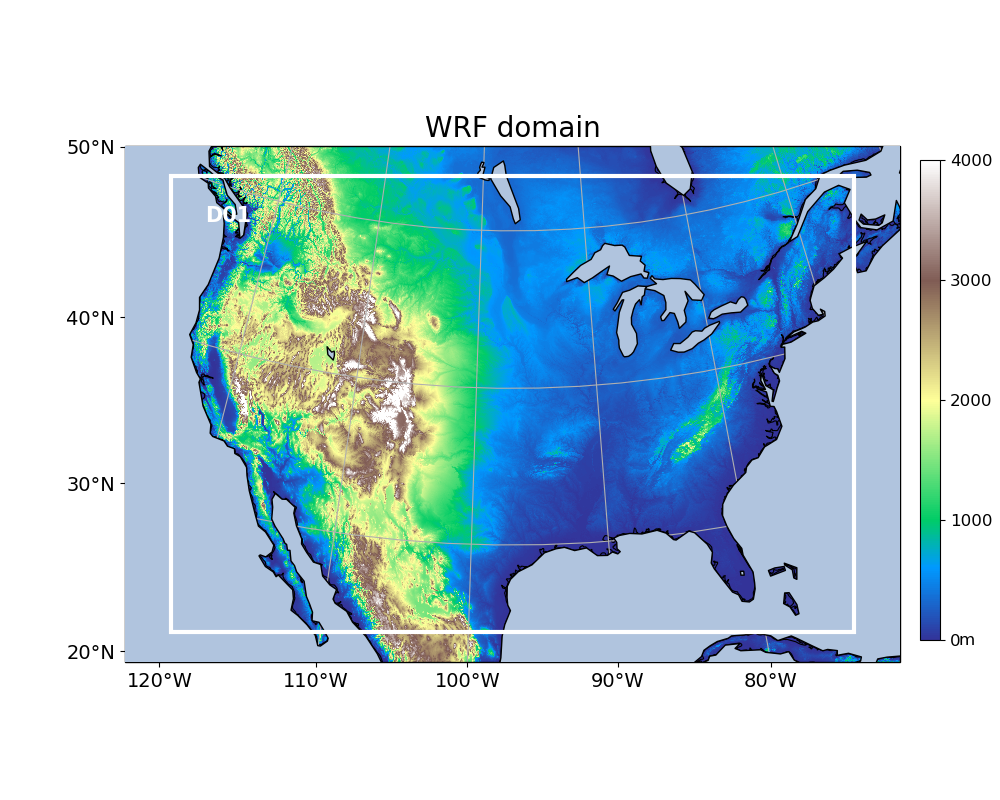
\includegraphics[width=11cm]{./figures/us_domain.png}
\caption{WRF-Chem 模拟区域和地形高度(m),网格数为 350 $\times$ 290,水平分辨率为 12 km \\
Figure \ref{fig:us_domain}. Domain and terrain height (m) of the WRF-Chem simulation with 350 x 290 grid cells and a horizontal resolution of 12 km.}
\label{fig:us_domain}
\end{figure}



\subsection{闪电氮氧化物的筛选条件}

首先我们使用恒定值网格化法,将公式(\ref{eq:AMF_LNO2})所得的LNO$_x$垂直柱浓度(V$_{\ch{LNO_x}}$)分配至0.05$^{\circ}$ $\times$ 0.05$^{\circ}$网格\citep{Kuhlmann.2014}。
接着在 1$^{\circ}$ $\times$ 1$^{\circ}$的网格中进行分析,要求每个网格至少有50个有效的0.05$^{\circ}$ $\times$ 0.05$^{\circ}$网格数据,从而最小化噪点数据。
具体筛选条件和主要计算步骤如下。

云辐射分数(CRF,CRF $\geq$ 70\%,CRF $\geq$ 90\%,CRF = 100\%)和 云压(CP,CP $\leq$ 650 hPa)
通常是OMI像素是否包含深对流云的判断标准\citep{Ziemke.2009,Choi.2014,Pickering.2016}。
% 不同CRF对LNO$_x$产品的影响将在\ref{subsec:retrieval_polluted}节探讨。
此外,我们将另一个云分数 (CF)标准应用于 WRF-Chem 的模拟结果,以确保对流被成功模拟。
具体而言,CF是由 Xu-Randall 方法计算的 350--400 hPa 之间的最大云分数\citep{Xu.1996,Strode.2017}。
我们根据\citet{Strode.2017}的建议,选择350--400 hPa的CF $\geq$ 40\%来判断模拟所处的网格是多云或晴空,
可避免模拟高云中的偏差。

除了云特性之外,OMI能探测到新生LNO$_x$的另一条件为一段时间内有足够的闪电或闪击。
其中,时间窗口 (t$_{window}$) 是 OMI 过境之前的时间段。
\citet{Lapierre.2020}利用1$^{\circ}$ $\times$ 1$^{\circ}$网格的对角线长度和OMI过境时美国大陆上空500--100 hPa的平均风速计算得到t$_{window}$为2.4 h。
同时,\citet{Lapierre.2020}定义在t$_{window}$时间段内,至少发生2400次闪电或8160次闪击的网格才能提供足够的LNO$_x$给OMI探测。
\citet{Bucsela.2019}的研究表明,低频率的闪电具有更高的LNO$_x$产率,而该段数据在\citet{Lapierre.2020}研究中被剔除。
通过比较使用每个网格至少2400次闪电和至少1次闪电的标准所得结果,我们也得到相同的结论(图\ref{fig:us_flash_threshold})。
由于我们的研究重点是开发一种新的AMF,并将计算结果与使用类似闪电阈值的其他产品进行比较\citep{Pickering.2016,Lapierre.2020},
因此我们接下来使用相同的至少2400次闪电标准来进行结果分析。


\begin{figure}[H]
    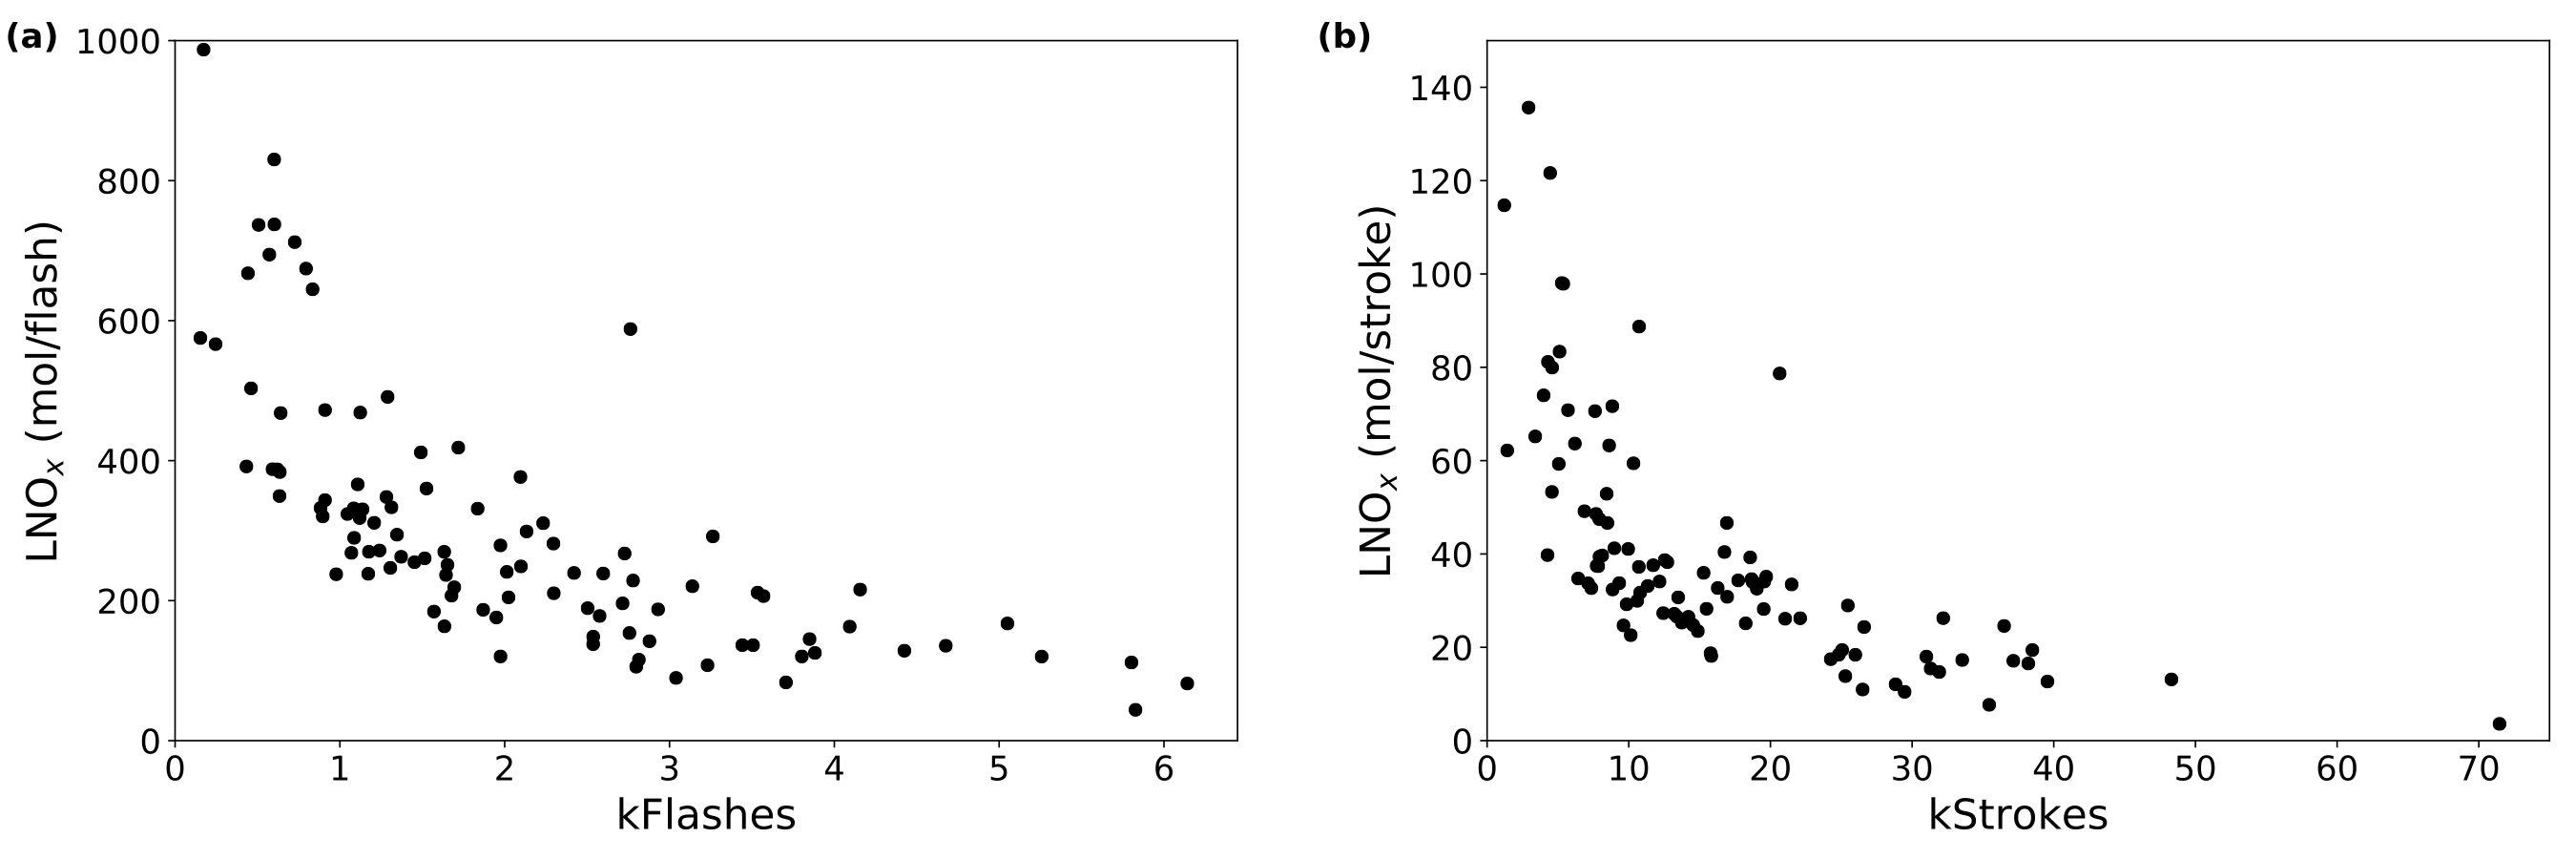
\includegraphics[width=15cm]{./figures/us_flash_threshold.png}
    \caption{
    (a) 每日 LNO$_x$ 产率与 ENTLN 总闪的关系,筛选条件为CRF $\geq$ 90\% 且1$^{\circ}$ $\times$ 1$^{\circ}$网格中至少有1次闪电;
     (b) 与 (a) 相同,但针对闪击。\\
    Figure \ref{fig:us_flash_threshold}. (a) Daily LNO$_x$ production efficiencies versus ENTLN total flashes data, with CRF $\geq$ 90\% and a flash threshold of 1 flash box$^{-1}$.
    (b) Same as (a) but for strokes.}
    \label{fig:us_flash_threshold}
\end{figure}


为确保WRF-Chem成功模拟出闪电,并考虑到闪电参数化的不确定性,我们将每个1$^{\circ}$ $\times$ 1$^{\circ}$网格模拟的总闪电(TL)阈值设置为1000,该阈值低于ENTLN闪电观测使用的阈值。
针对除LNO$_2$之外的其他NO$_2$源,我们定义了模拟的云上闪电NO$_2$柱浓度($V_{\ch{LNO2}}$)
与云上NO$_2$柱浓度($V_{\ch{NO2Vis}}$)之比,来判断OMI是否可以检测到足够的LNO$_2$,
该比率$\geq$50\%表明云层上方超过一半的NO$_x$具有LNO$_x$源。
此外,还需考虑氧化有关的NO$_2$寿命,
\citet{Nault.2017}的研究表明NO$_2$在对流附近的寿命($\tau$)为$\approx$3 h,故NO$_2$的初始值可由式(\ref{eq:inition})求解。

\begin{equation} \label{eq:inition}
NO_2(0) = NO_2(\mathrm{OMI})\ e^{0.5t/\tau}
\end{equation}

其中$NO_2(0)$是在时间 t=0 时刻排放的NO$_2$摩尔数,$NO_2(\mathrm{OMI})$是在 OMI 过境时间测得的NO$_2$摩尔数,
0.5t是穿过网格的时间,即1.2 h(假设闪电出现在每个1$^{\circ}$ $\times$ 1$^{\circ}$网格的中心)。
每个网格的V$_{\ch{LNO_x}}$为网格中所有0.05$^{\circ}$ $\times$ 0.05$^{\circ}$像素的V$_{\ch{LNO_x}}$平均值,
然后乘以网格的面积得到LNO$_x$摩尔数。
最后,有两种方法可用于估算季节性平均LNO$_2$每闪电、LNO$_x$每闪电、LNO$_x$每闪击和 LNO$_x$每闪击:

(1)求和法,将LNO$_x$的总和除以5--8月中每个1$^{\circ}$ $\times$ 1$^{\circ}$网格里发生的闪电或闪击总数;

(2)线性回归方法,将线性回归应用于每日LNO$_x$和闪电或闪击平均值。

% \subsection{适合反演闪电氮氧化物的条件} \label{subsec:criteria}

根据以上条件,我们定义了六种不同的筛选条件组合(表\ref{table:Abbreviations}),并使用线性回归法应用于原始数据。

\begin{table*}[htbp]
\caption{本研究中使用的标准的缩写定义\\Table \ref{table:Abbreviations}. Definitions of the abbreviations for the criteria used in this study.}
\scriptsize
\begin{tabular}{ll}
\hline
缩写$^a$ & 全称 [来源] \\
\hline
CRF                             & 云辐射分数 Cloud radiance fraction [OMI] \\
CP                              & 云压Cloud pressure [OMI] \\
CF                              & 云分数 Cloud fraction [WRF-Chem] \\
TL                              & 总闪电数 Total lightning flashes [WRF-Chem] \\
ratio                           & $V_{\ch{LNO2}}$ / $V_{\ch{NO2Vis}}$ [WRF-Chem] \\
CRF$\alpha$\_ENTLN                   & CRF $\geq$ $\alpha$ + ENTLN 闪电(闪击) $\geq$ 2400(8160) [ENTLN]\\
CRF$\alpha$\_CF40\_ENTLN              & CRF $\geq$ $\alpha$ + ENTLN 闪电(闪击) $\geq$ 2400(8160) + CF $\geq$ 40\% \\
CRF$\alpha$\_ENTLN\_TL1000            & CRF $\geq$ $\alpha$ + ENTLN 闪电(闪击) $\geq$ 2400(8160) + TL $\geq$ 1000 \\
CRF$\alpha$\_CF40\_ENTLN\_TL1000      & CRF $\geq$ $\alpha$ + ENTLN 闪电(闪击) $\geq$ 2400(8160) + CF $\geq$ 40\% + TL $\geq$ 1000 \\
CRF$\alpha$\_ENTLN\_TL1000\_ratio50   & CRF $\geq$ $\alpha$ + ENTLN 闪电(闪击) $\geq$ 2400(8160) + TL $\geq$ 1000 + ratio $\geq$ 50\% \\
CRF$\alpha$\_CF40\_ENTLN\_TL1000\_ratio50 & CRF $\geq$ $\alpha$ + ENTLN 闪电(闪击) $\geq$ 2400(8160) + CF $\geq$ 40\% + TL $\geq$ 1000 + ratio $\geq$ 50\% \\
CRF$\alpha$\_ENTLN1(3.4)\_TL1\_ratio50    & CRF $\geq$ $\alpha$ + ENTLN 闪电(闪击) $\geq$ 1(3.4) + TL $\geq$ 1 + ratio $\geq$ 50\% \\
\hline
\end{tabular}
\begin{tablenotes}
\footnotesize
\item $^a$ $\alpha$有三种选择:70\%、90\%以及100\%。
\item $^a$ $\alpha$ has three options: 70\%, 90\% and 100\%.
\end{tablenotes}
\label{table:Abbreviations}
\end{table*}


\begin{table*}[htbp]
\caption{根据表\ref{table:Abbreviations}中的定义得到的LNO$_x$产率\\Table \ref{table:conditions} LNO$_x$ production efficiencies for different combinations of criteria defined in Table \ref{table:Abbreviations}.}
\scriptsize
\begin{tabular}{lccccc}
\hline
条件$^a$ & ENTLN类型$^b$ & LNO$_x$每闪电 or LNO$_x$每闪击 & R值 & 截距 (10$^{6}$mol) & 天数$^c$ \\
\hline
CRF90\_ENTLN                        & 闪电  & 52.1 $\pm$ 51.1 & 0.20 & 0.21  & 99 \\
CRF90\_CF40\_ENTLN                  & 闪电  & 84.2 $\pm$ 31.5 & 0.54 & -0.04 & 70 \\
CRF90\_ENTLN\_TL1000                & 闪电  & 61.9 $\pm$ 49.1 & 0.27 & 0.33  & 83 \\
CRF90\_CF40\_ENTLN\_TL1000          & 闪电  & 63.4 $\pm$ 52.9 & 0.38 & 0.26  & 38 \\
CRF90\_ENTLN\_TL1000\_ratio50       & 闪电  & 54.5 $\pm$ 48.1 & 0.25 & 0.39  & 81 \\
CRF90\_CF40\_ENTLN\_TL1000\_ratio50 & 闪电  & 90.0 $\pm$ 65.0 & 0.46 & 0.15  & 32 \\
CRF90\_ENTLN                        & 闪击 & 6.7 $\pm$ 4.1 & 0.31 & 0.23  & 102 \\
CRF90\_CF40\_ENTLN                  & 闪击 & 10.3 $\pm$ 3.6 & 0.55 & 0.08 & 79 \\
CRF90\_ENTLN\_TL1000                & 闪击 & 7.5 $\pm$ 5.1 & 0.29 & 0.38  & 94 \\
CRF90\_CF40\_ENTLN\_TL1000          & 闪击 & 8.6 $\pm$ 6.2 & 0.39 & 0.27  & 46 \\
CRF90\_ENTLN\_TL1000\_ratio50       & 闪击 & 7.0 $\pm$ 4.8 & 0.29 & 0.42  & 93 \\
CRF90\_CF40\_ENTLN\_TL1000\_ratio50 & 闪击 & 8.9 $\pm$ 7.0 & 0.39 & 0.31  & 40 \\
\hline
\label{table:conditions}
\end{tabular}
\begin{tablenotes}
\footnotesize
\item $^a$ 定义见表\ref{table:Abbreviations}。
\item $^b$ ENTLN阈值为OMI过境前2.4小时内 1$^{\circ}$ $\times$ 1$^{\circ}$网格中闪电至少2400次和闪击至少8160次。
\item $^c$ 2014年5--8月中有效的天数。
\item $^a$ These conditions are defined in Table \ref{table:Abbreviations}.
\item $^b$ The thresholds of ENTLN data are 2400 flashes box$^{-1}$ and 8160 strokes box$^{-1}$ during the period of 2.4 h before OMI overpass time.
\item $^c$ The number of valid days with specific criteria in MJJA 2014.
\end{tablenotes}
\end{table*}


在CRF90\_ENTLN条件下,有效闪电(闪击)数据对应共有99(102)天。
以闪电类ENTLN数据为例,在 CRF90\_ENTLN\_TL1000\_ratio50 条件下,有效天数从 99 减少至 81,而LNO$_x$产率从 52.1 $\pm$ 51.1 mol每闪电增加到 54.5 $\pm$ 48.1 mol每闪电。
该结果与 CRF90\_ENTLN\_TL1000 条件下所得的结果几乎相同。
尽管这表明TL筛选条件已足够严格,但最好包括云上LNO$_2$占比的筛选条件,以防不同的AMF方法中存在一些例外情况。
由于 CF $\geq$ 40\% 会导致有效数据和产率急剧下降,因此我们仅仅使用 CRF 对数据进行筛选。
最后,我们选择至少2400次闪电或至少8160次闪击,TL $\geq$ 1000 和云上LNO$_2$占比 $\geq$ 50\% 作为阈值,来探索三种不同 CRF 条件(CRF $\geq$ 70\%、CRF $\geq$ 90\% 和 CRF = 100\%)对 LNO$_x$ 估算产生的影响(表\ref{table:CRFs})。
当CRF 标准从 70\% 增加到 90\% 和 100\%时,针对闪电类型的LNO$_x$产率 从35.7 $\pm$ 36.8 mol每闪电增加到 54.5 $\pm$ 48.1 mol每闪电,然后再降低到20.8 $\pm$ 37.4 mol每闪电,而针对闪击类型的LNO$_x$产率从4.1 $\pm$ 3.9 mol每闪击提高到 7.0 $\pm$ 4.8 mol每闪击,然后再次下降到2.6 $\pm$ 4.0 mol每闪击(表\ref{table:CRFs})。
当 CRF 从 90\% 增加到 100\% 时LNO$_x$ 产率降低,这是因为闪电密度较高而 LNO$_x$ 较少。
CRF 从 70\% 增加到 90\% 引起的 LNO$_x$ 产率增大,该现象与\citet{Pickering.2016}的结果相反。
这是由于我们的方法中考虑了从边界层传输的 NO$_2$ 污染的影响。
虽然在 CRF $\geq$ 70\% 的地区经常观察到 NO$_x$ 增强\citep{Pickering.2016},但考虑到中低浓度 NO$_2$ 的污染并与\citet{Pickering.2016}和\citet{Lapierre.2020}的结果进行比较,以下分析将基于 CRF $\geq$ 90\% 标准进行讨论分析。

\begin{table*}[htbp]
\caption{在相同ENTLN阈值,TL $\geq$ 1000 和云上LNO$_2$占比 $\geq$ 50\%的条件下,不同云辐射分数阈值对应的LNO$_x$产率 \\
Table \ref{table:CRFs}. LNO$_x$ production efficiencies for different thresholds of CRF with coincident ENTLN data, TL $\geq$ 1000 and ratio $\geq$ 50\%.}
\footnotesize
\begin{tabular}{cccccc}
\hline
云辐射分数 (\%) & ENTLN类型$^a$    & LNO$_x$每闪电或LNO$_x$每闪击
& R值    & 截距 (10$^{5}$mol)  & 天数$^b$ \\
\hline
70  & 闪电  & 35.7  $\pm$ 36.8 & 0.21 & 4.91 & 85 \\
90  & 闪电  & 54.5  $\pm$ 48.1 & 0.25 & 3.90 & 81 \\
100 & 闪电  & 20.8  $\pm$ 37.4 & 0.13 & 5.67 & 71 \\
70  & 闪击 & 4.1   $\pm$ 3.9  & 0.21 & 5.16 & 96 \\
90  & 闪击 & 7.0   $\pm$ 4.8  & 0.29 & 4.16 & 93 \\
100 & 闪击 & 2.6   $\pm$ 4.0  & 0.14 & 5.41 & 82 \\
\hline
\end{tabular}
\begin{tablenotes}
\footnotesize
\item $^a$ENTLN阈值为 OMI 过境前 2.4 小时内每个网格至少 2400 次闪电或8160 次闪击。
\item $^b$2014年5--8月对应筛选条件下有效天数。
\item $^a$The thresholds of ENTLN data are 2400 flashes box$^{-1}$ and 8160 strokes box$^{-1}$ during the period of 2.4 h before OMI overpass time.
\item $^b$The number of valid days with specific criteria in MJJA 2014.
\end{tablenotes}
\label{table:CRFs}
\end{table*}

\subsection{闪电氮氧化物的产率}
% \subsection{基于不同反演方法的结果对比}

% \citet{Lapierre.2020}基于 BEHR NO$_2$ 产品得出 LNO$_2$ 产量,
为了使本研究的结果与\citet{Pickering.2016}和\citet{Lapierre.2020}的结果具有可比性,我们选择 NO$_2$  而不是 NO$_x$  来计算每次闪电的产量(产率)。
在图\ref{fig:us_pe_timeseries}中,根据 CRF $\geq$ 90\% 和每 2.4 h 2400次闪电的阈值,绘制了2014年5--8月美国大陆每天 NO$_2$Vis、LNO$_2$Vis、LNO$_2$ 和 LNO$_2$Clean 产率的时间序列图。
其中,LNO$_2$ 产率大多在 20 至 80 mol每闪电的范围内,LNO$_2$Vis 产率小于LNO$_2$产率,因为后者包含了云下的LNO$_2$。
\citet{Pickering.2016}的GMI模拟结果表明,25--30\%的LNO$_x$柱浓度位于云压以下,
而我们的WRF-Chem模拟结果显示该比例为 56\% $\pm$ 20\%。
云属性对 LNO$_x$ 产率的影响将在\ref{sec:uncertainty}节中进行更详细地讨论。
总体而言,估算得到的每日产率顺序为LNO$_2$Clean > LNO$_2$ > NO$_2$Vis > LNO$_2$Vis。
通过NO$_2$Vis 和 LNO$_2$Vis 估算得到的产率之间的相对差异($\Delta$PE)表明有一定量的背景 NO$_2$ 存在于云层之上。
总体而言,该 $\Delta$PE 的趋势与 NO$_2$Vis 和 LNO$_2$Clean 之间的$\Delta$PE 一致。
当区域污染严重时(NO$_2$Vis 和 LNO$_2$Vis 之间的 $\Delta$PE > 200\%),
基于 NO$_2$Vis 和 LNO$_2$Clean 的产率被显著高估。
换言之,NO$_2$Vis 和 LNO$_2$Clean 对背景 NO$_2$ 更为敏感,
且在高污染地区NO$_2$Vis的高估程度大于 LNO$_2$Clean,而在其他大多数地区通常相反。

\begin{figure}[H]
\centering
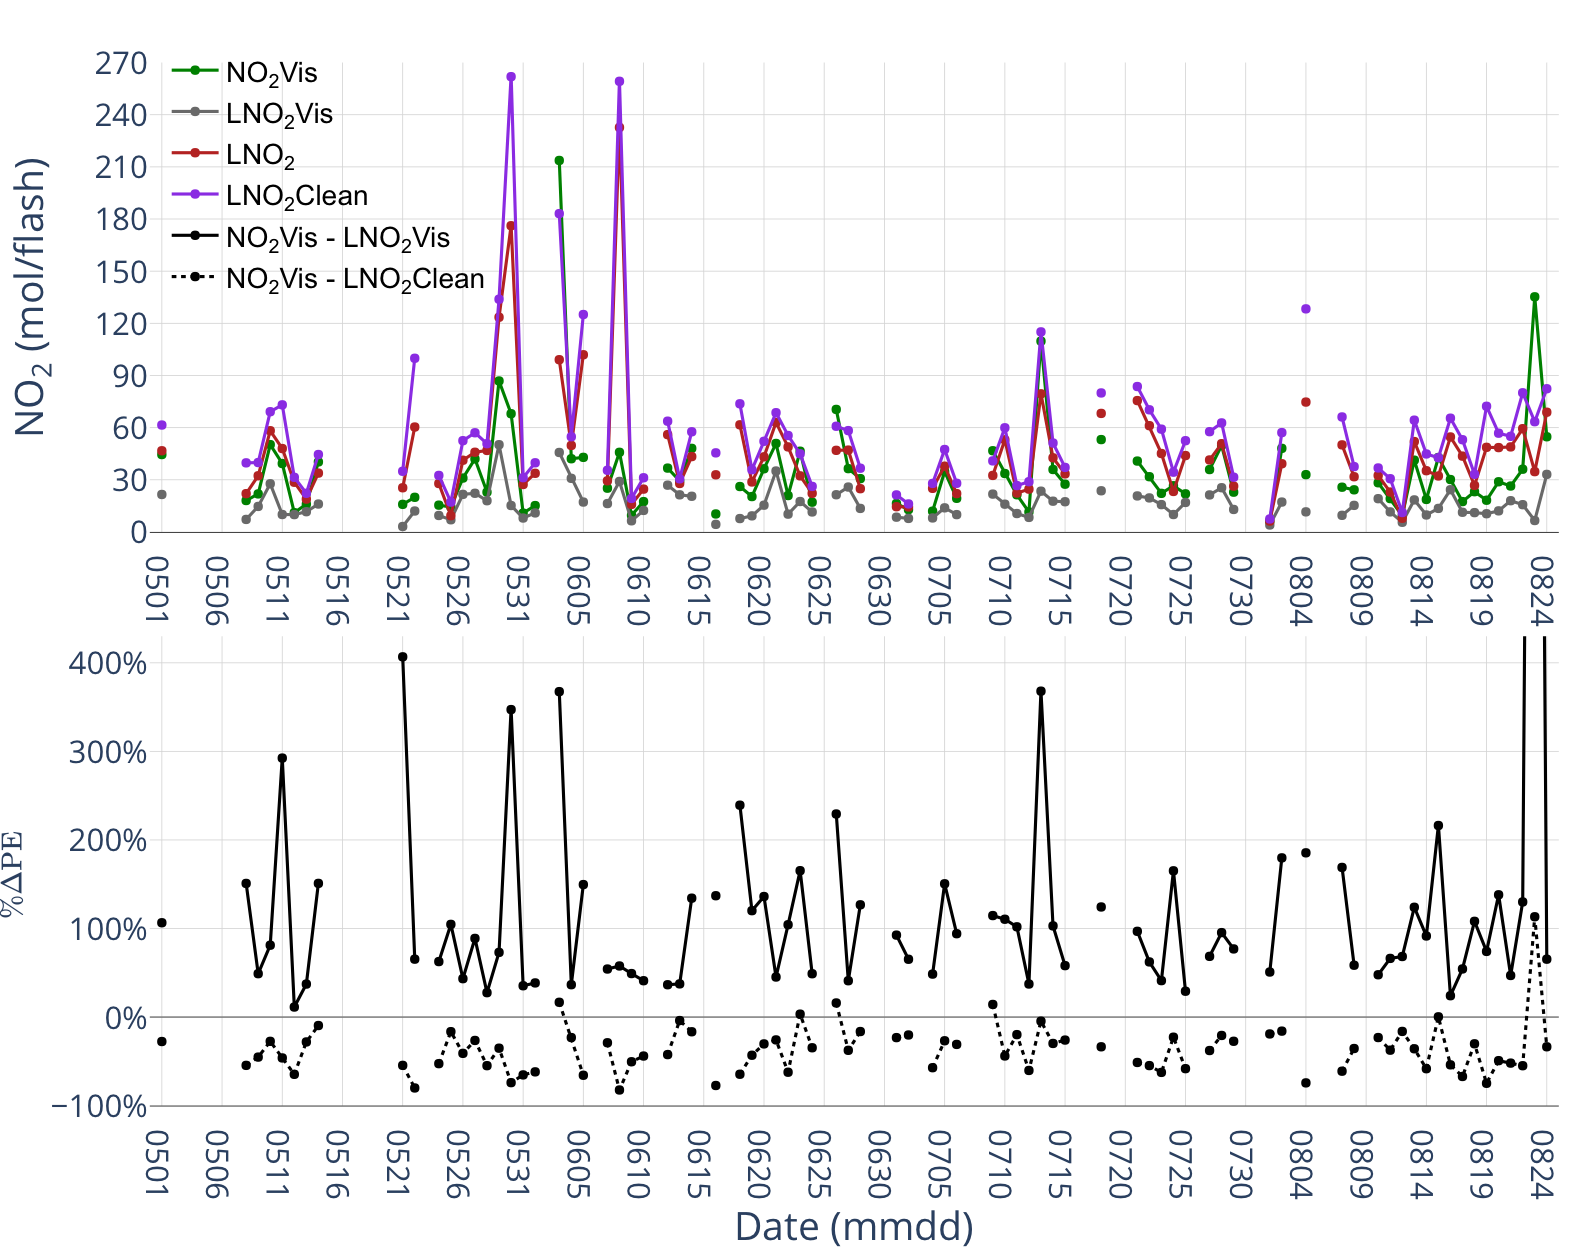
\includegraphics[width=12cm]{./figures/us_pe_timeseries.png}
\caption{(上图)NO$_2$Vis、LNO$_2$Vis、LNO$_2$ 和 LNO$_2$Clean产率的时间序列(2014年5--8月美国大陆),筛选条件为CRF $\geq$ 90\% 和每 2.4 小时 至少2400 次闪电;
(下图)在CRF$\geq$ 90\%的条件下,NO$_2$Vis 和 LNO$_2$Vis 之间百分比差异以及 NO$_2$Vis 和 LNO$_2$Clean 之间百分比差异的时间序列。
8 月 23 日黑点的值(未显示)为 1958\%。\\
Figure \ref{fig:us_pe_timeseries}. (top) Time series of NO$_2$Vis, LNO$_2$Vis, LNO$_2$ and LNO$_2$Clean production per day over the CONUS for MJJA 2014 with CRF $\geq$ 90\% and a flash threshold of 2400 flashes per 2.4 h.
(bottom) Time series of the percent differences between NO$_2$Vis and LNO$_2$Vis and the percent differences between NO$_2$Vis and LNO$_2$Clean with CRF $\geq$ 90\%.
The value of black dot on August 23 (not shown) is 1958\%.}
\label{fig:us_pe_timeseries}
\end{figure}

图\ref{fig:us_pe_linear}为ENTLN 数据与 NO$_2$Vis、LNO$_2$Vis、LNO$_2$ 和 LNO$_2$Clean的线性回归,
其筛选条件与图 \ref{fig:us_pe_timeseries} 相同。
LNO$_2$Clean 产率为 25.2 $\pm$ 22.3 mol NO$_2$ 每闪电(相关系数为0.25)
和 2.3 $\pm$ 2.1 mol NO$_2$每闪击(相关系数为0.22)。
如图\ref{fig:us_pe_timeseries}所示,NO$_2$Vis产率和LNO$_2$Clean产率之间的正百分比差异发生的频率远低于负差异的发生频率。
因此,NO$_2$Vis产率(17.1 $\pm$ 17.2 mol NO$_2$ 每闪电和0.4 $\pm$ 1.0 mol NO$_2$ 每闪击)
小于使用线性回归方法得到的 LNO$_2$Clean产率。

为了将我们的结果与\citet{Lapierre.2020}的结果进行比较,
我们选择了CP $\leq$ 650 hPa、TL $\geq$ 1000 和 ratio $\geq$ 50\% 的条件。
但是,我们得到的NO$_2$Vis(3.8 $\pm$ 0.5 mol每闪击)仍大于\citet{Lapierre.2020}的1.6 $\pm$ 0.1 mol每闪击。
这可能是由两者使用不同版本的伯克利高分辨率(BEHR)算法引起的,\citet{Lapierre.2020}使用的是BEHR v3.0A,我们的算法基于BEHR v3.0B \citep{Laughner.2019a}。
两个版本中$S_{\ch{NO2}}$均来自于NASA标准产品v3,BEHR v3.0B 的主要改进如下:

(1)使用最接近 OMI 过境时间的廓线,而不是 OMI 过境之前的最后一个时刻的廓线;

(2)使用可变的对流层顶高度,而不是固定的200 hPa 对流层顶;

(3)根据\citet{Zhou.2009}的方法计算地表气压。

% 详细的更新日志见\url{https://github.com/CohenBerkeleyLab/BEHR-core/blob/master/Documentation/Changelog.txt}。
此外,\citet{Lapierre.2020}使用了月平均NO$_2$廓线,而我们的研究使用了日廓线,并且我们将WRF-Chem 输出的间隔调整为 30 min,
这比BEHR 每日产品(1 h)输出间隔更短,但 AMF 可能还会受到不同 NO$_2$ 廓线的影响。
鉴于这些因素,我们在所得数据的基础上来比较不同的方法,以尽量减少这些影响。

\begin{figure}[H]
    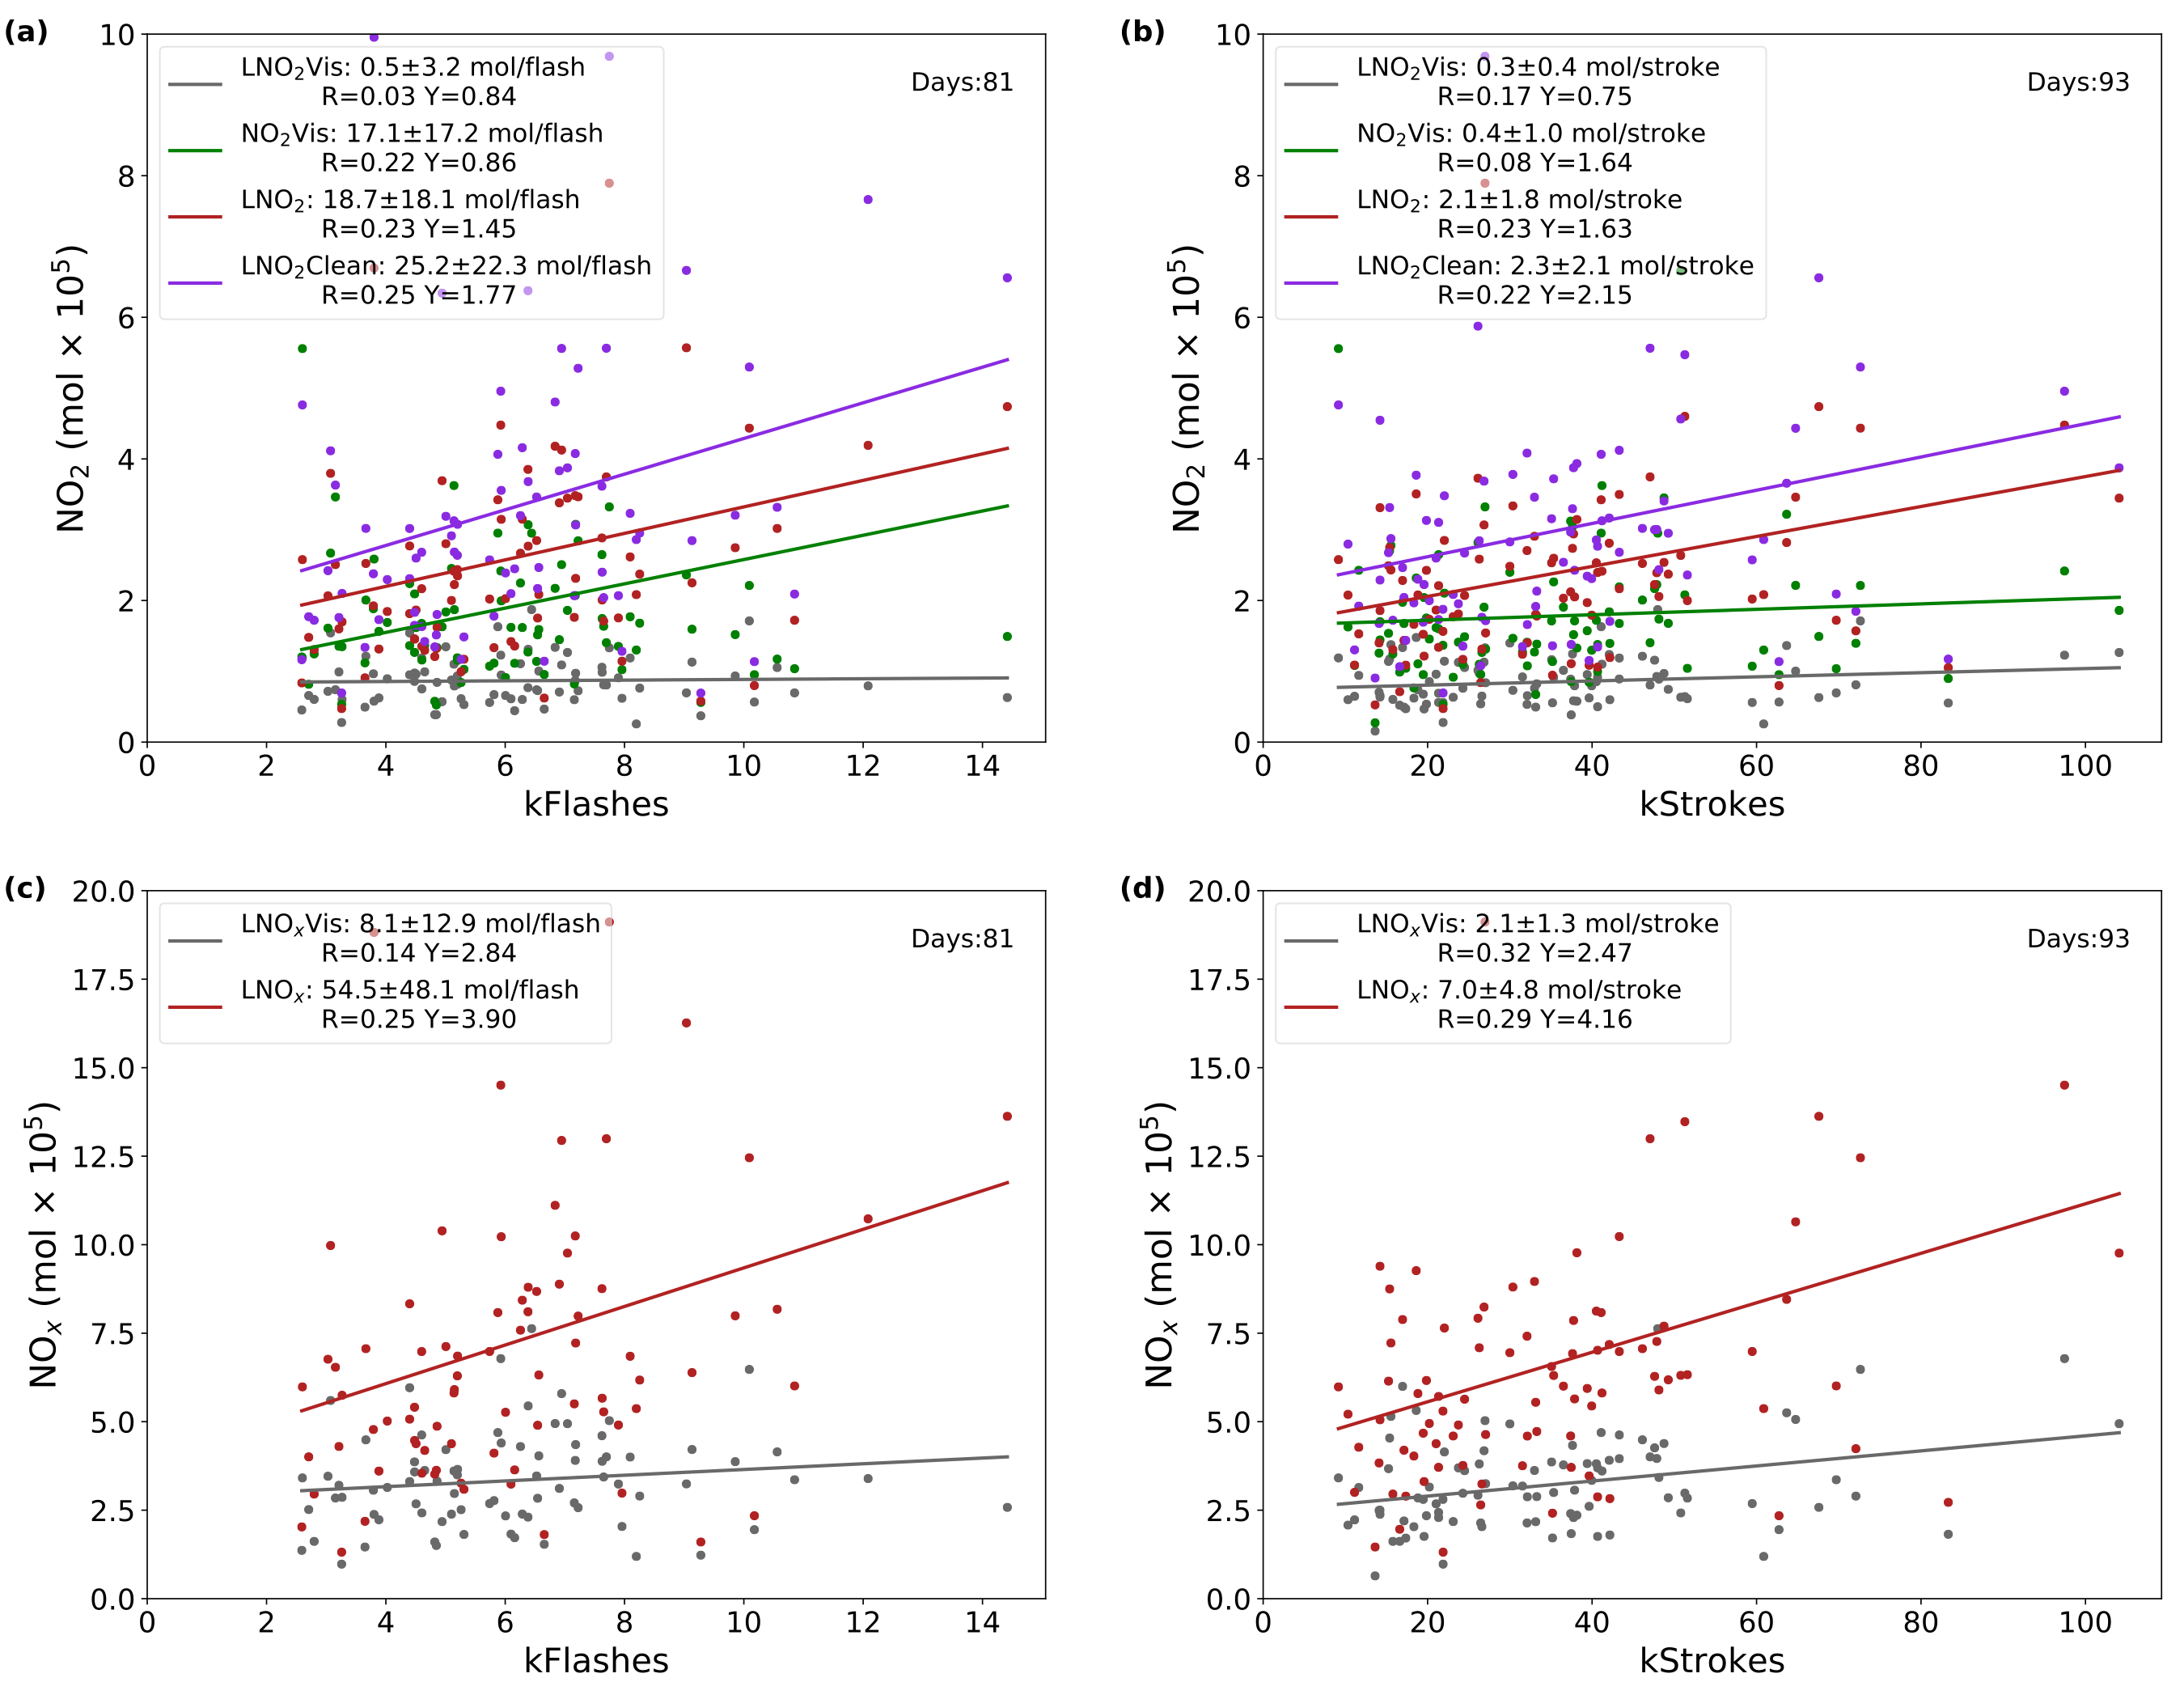
\includegraphics[width=13cm]{./figures/us_pe_linear.png}
    \caption{(a)每日 NO$_2$Vis、LNO$_2$Vis、LNO$_2$ 和 LNO$_2$Clean 与 ENTLN 总闪的关系;
    (b)与(a)相同,但针对闪击数据;
    (c)每日LNO$_x$Vis 和 LNO$_x$ 与总闪的关系;
    (d)与(c)相同,但针对闪击数据。\\
    Figure \ref{fig:us_pe_linear}.
    (a) Daily NO$_2$Vis, LNO$_2$Vis, LNO$_2$ and LNO$_2$Clean versus ENTLN total flashes data.
    (b) Same as (a) but for strokes.
    (c) Daily LNO$_x$Vis and LNO$_x$ versus total flashes.
    (d) Same as (c) but for strokes.}
    \label{fig:us_pe_linear}
\end{figure}

结果表明,LNO$_2$产率(18.7 $\pm$ 18.1 mol每闪电,2.1 $\pm$ 1.8 mol每闪击)介于 LNO$_2$Clean产率 和 NO$_2$Vis产率之间,
与图 \ref{fig:us_pe_timeseries} 中的日结果一致。
此外,基于每日求和值的线性回归结果得到的LNO$_x$产率为114.8 $\pm$ 18.2 mol每闪电(或17.8 $\pm$ 2.9 mol每闪击),
该结果大于\citet{Pickering.2016}的91 mol每闪电。
这一差异可能是由地理位置、闪电数据和化学模式所共同导致的。
在 CRF $\geq$ 90\% 下,求和法得到LNO$_2$产率为 46.2 $\pm$ 35.1 mol 每闪电和 9.9 $\pm$ 8.1 mol 每闪电,
而 LNO$_x$ 产率为 125.6 $\pm$ 95.9 mol 每闪电和 26.7 $\pm$ 21.6 mol 每闪电(图\ref{fig:us_pe_sum})。
其中美国东南部的 LNO$_2$和 LNO$_x$ 产率均较高(由图\ref{fig:us_pe_sum}中的红框表示,25--37$^{\circ}$ N,75--95$^{\circ}$ W),这与\citet{Lapierre.2020} 和 \citet{Bucsela.2019}的研究结果相一致。
而与图\ref{fig:us_pe_timeseries}相比,图\ref{fig:us_delta}a--b显示
NO$_2$Vis产率和 LNO$_2$Vis产率之间的一些较大差异,这与我们对污染区域的预期一致。
同时,LNO$_2$ 和 NO$_2$Vis产率之间的差异取决于背景 NO$_2$、上升气流的强度和廓线分布。
负差异是由上升气流携带的背景 NO$_2$ 污染引起的,
而云下 LNO$_2$ 的部分导致LNO$_2$产率高于NO$_2$Vis产率(图\ref{fig:us_delta}c)。
图\ref{fig:us_delta}d显示 LNO$_2$Vis在LNO$_2$中占比为 10--80\%,
这可能是由云层的高度和 LNO$_2$ 的廓线造成的。
如果云压在300 hPa附近,由于云层的覆盖,该比值将更小。
因此,LNO$_x$的估算需要更好地了解LNO$_2$和云下LNO$_x$的垂直分布。


\begin{figure}[H]
\centering
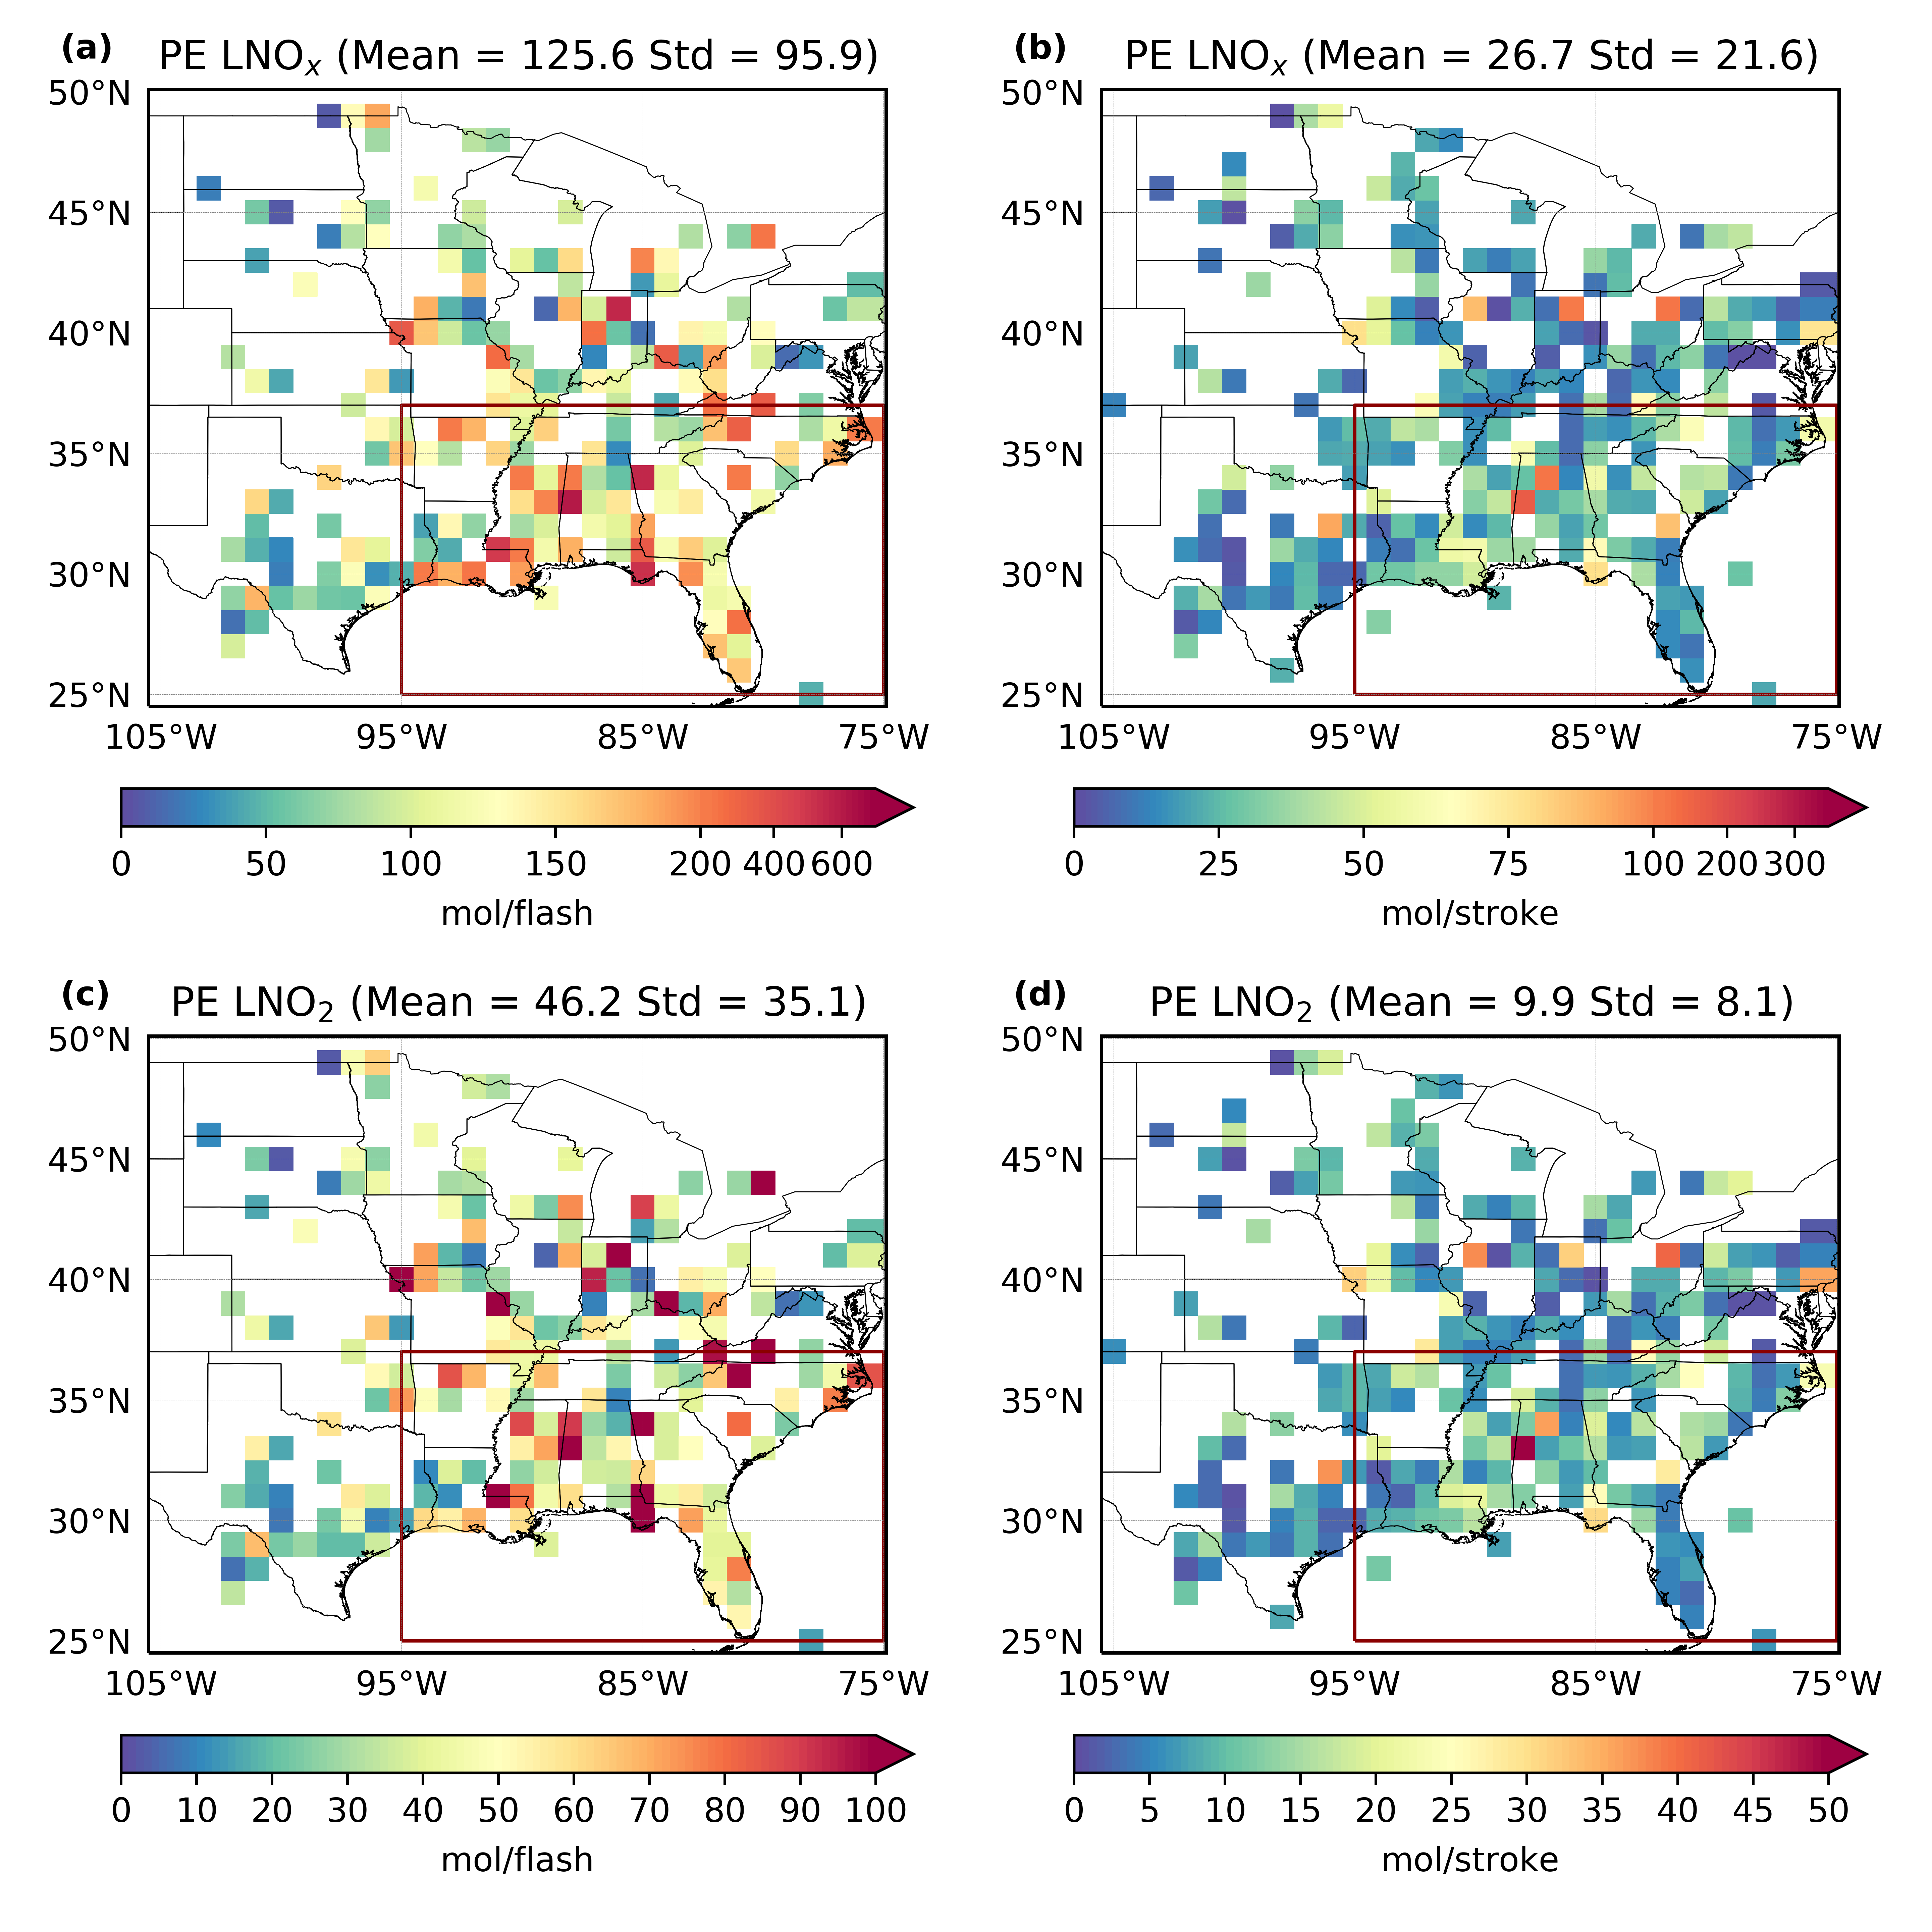
\includegraphics[width=13cm]{./figures/us_pe_sum.png}
\caption{(a,c)在CRF $\geq$ 90\%条件下,2014年5--8月 1$^{\circ}$ $\times$ 1$^{\circ}$ LNO$_x$ 和LNO$_2$的平均产率分布图;
     (b,d) 与 (a,c) 相同,但针对闪击数据。
     a--d中的红框表示美国东南部。\\
     Figure \ref{fig:us_pe_sum}. (a) and (c) Maps of 1$^{\circ}$ $\times$ 1$^{\circ}$ gridded values of mean LNO$_x$
    and LNO$_2$ production per flash with CRF $\geq$ 90\% for MJJA 2014.
    (b) and (d) Same as (a) and (c) except for strokes.
    The southeastern US is denoted by the red box in panels a--d.
}
\label{fig:us_pe_sum}
\end{figure}

\begin{figure}[H]
\centering
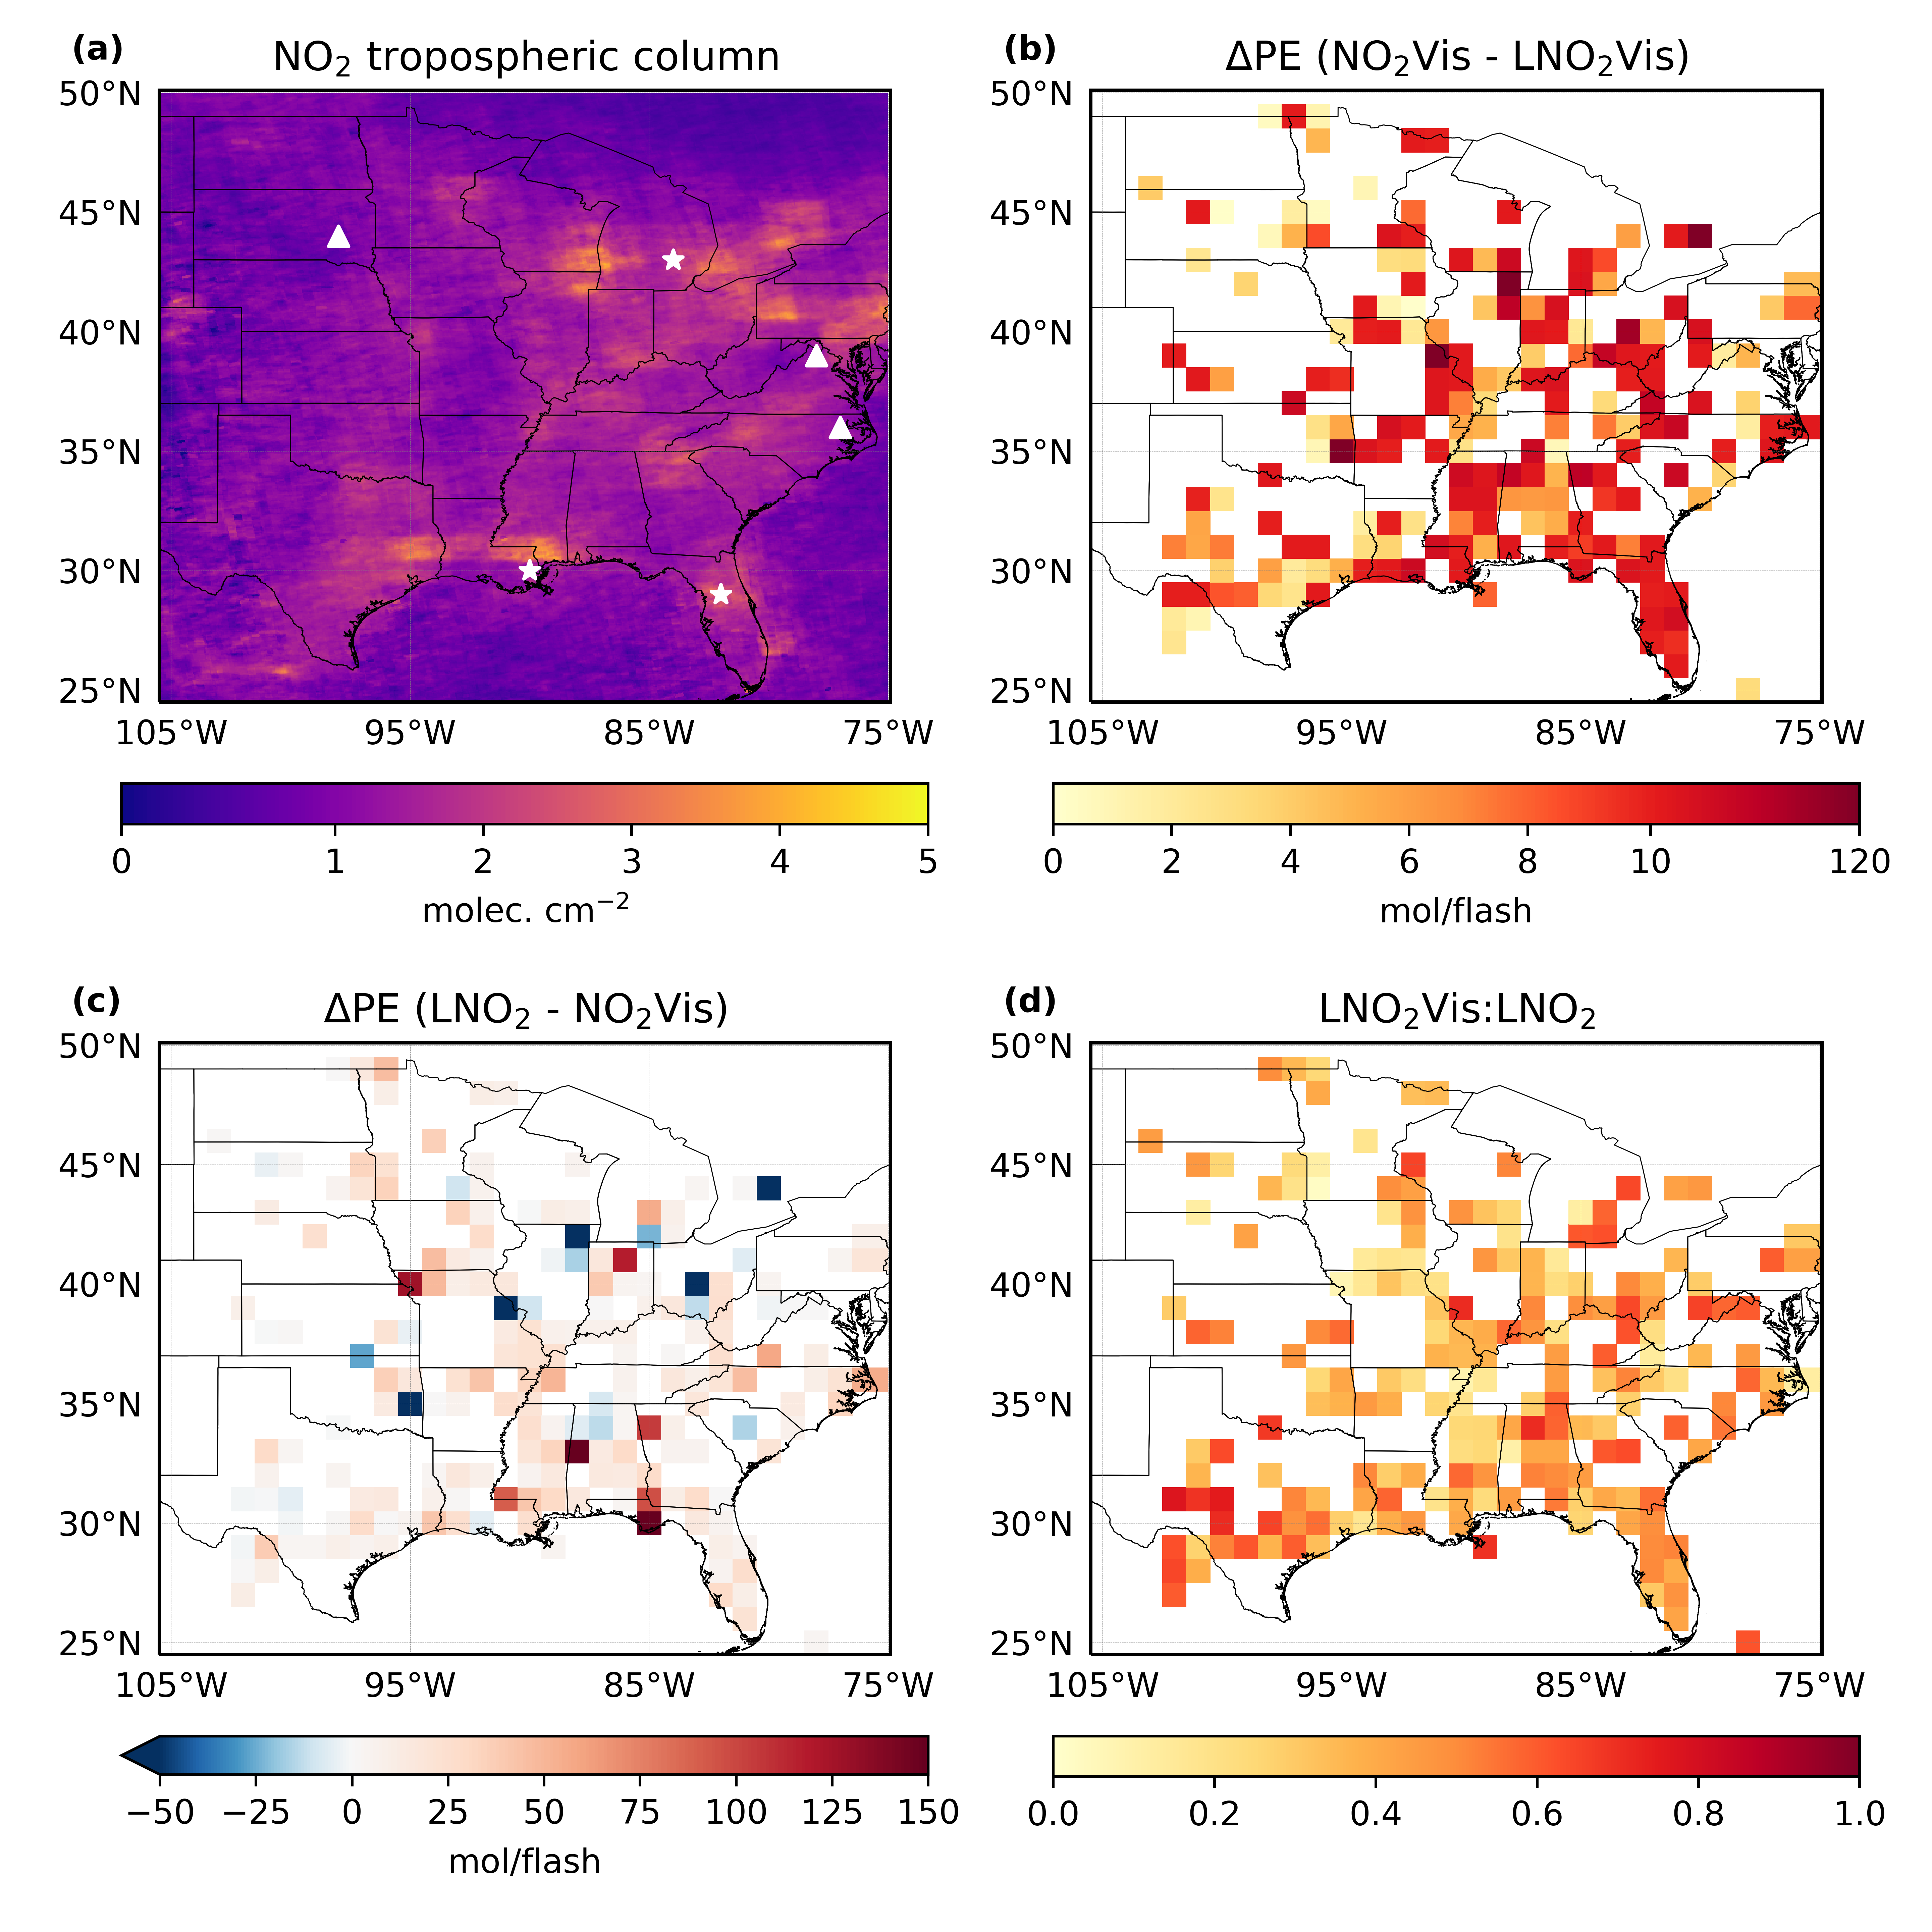
\includegraphics[width=13cm]{./figures/us_delta.png}
\caption{(a)2014年5--8月平均对流层NO$_2$柱浓度,
污染城市用星星表示:兰辛、新奥尔良和奥兰多,而清洁城市用三角形表示:休伦、查尔斯镇和塔伯勒;
(b)在CRF $\geq$ 90\%条件下,NO$_2$Vis 和 LNO$_2$Vis平均产率的差异;
(c)与(b)相同,但为 LNO$_2$ 和 NO$_2$Vis 之间的差异;
(d)LNO$_2$Vis 与 LNO$_2$ 的比例。\\
Figure \ref{fig:us_delta}.
(a) Mean (MJJA 2014) NO$_2$ tropospheric column.
Polluted cities are denoted by stars: Lansing, New Orleans and Orlando while clean cities are denoted by triangles: Huron, Charles Town and Tarboro.
(b) The differences of the estimated mean production efficiency between NO$_2$Vis and LNO$_2$Vis with CRF $\geq$ 90\%.
(c) The same differences as (b) but between LNO$_2$ and NO$_2$Vis.
(d) The ratio of LNO$_2$Vis to LNO$_2$.
}
\label{fig:us_delta}
\end{figure}
\FloatBarrier

\subsection{估算的影响因素及不确定性分析} \label{sec:uncertainty}

图\ref{fig:us_delta}表明我们方法对于LNO$_2$产率估算的改进在污染和清洁地区是不同的。
为了简化量化,我们选择了CRF = 100\%条件下,具有相似云上NO$_2$廓线($\approx$ 100 pptv)的六个网格,这样AMF之间的差异取决于较少的参数:

\begin{equation} \label{AMFLNO2_crf100}
AMF_{\ch{LNO2}} = \frac{\int_{p_{\ch{cloud}}}^{p_{\ch{tp}}} w_{\ch{cloudy}}(p) NO_2(p) \: dp}{\int_{p_{\ch{surf}}}^{p_{\ch{tp}}} LNO_2(p) \: dp}
\end{equation}

\begin{equation} \label{AMFNO2Vis_crf100}
AMF_{\ch{NO2Vis}} = \frac{\int_{p_{\ch{cloud}}}^{p_{\ch{tp}}} w_{\ch{cloudy}}(p) NO_2(p) \: dp}{\int_{p_{\ch{cld}}}^{p_{\ch{tp}}} NO_2(p) \: dp}
\end{equation}

\begin{equation} \label{AMFLNO2Clean_crf100}
AMF_{\ch{LNO2Clean}} = \frac{\int_{p_{\ch{cloud}}}^{p_{\ch{tp}}} w_{\ch{cloudy}}(p) LNO_2(p) \: dp}{\int_{p_{\ch{surf}}}^{p_{\ch{tp}}} LNO_2(p) \: dp}
\end{equation}

这些网格框包含图\ref{fig:us_delta}a中的污染城市(星形)和清洁城市(三角形)。
图\ref{fig:us_bkgd_comp}比较了污染和清洁网格内NO$_2$、背景 NO$_2$ 和背景 NO$_2$占比的平均廓线。
由于对流层上层LNO$_2$ 浓度高于背景 NO$_2$ 浓度,背景 NO$_2$ 与总 NO$_2$ 的比例曲线呈 C 形。
然而,随着背景 NO$_2$ 增加和 LNO$_2$ 的减少,图\ref{fig:us_bkgd_comp}e中的比例在云压和对流层顶之间存在峰值。
此外污染地区的对流层上层背景NO$_2$占比稳定且高于清洁地区。

\begin{figure}[H]
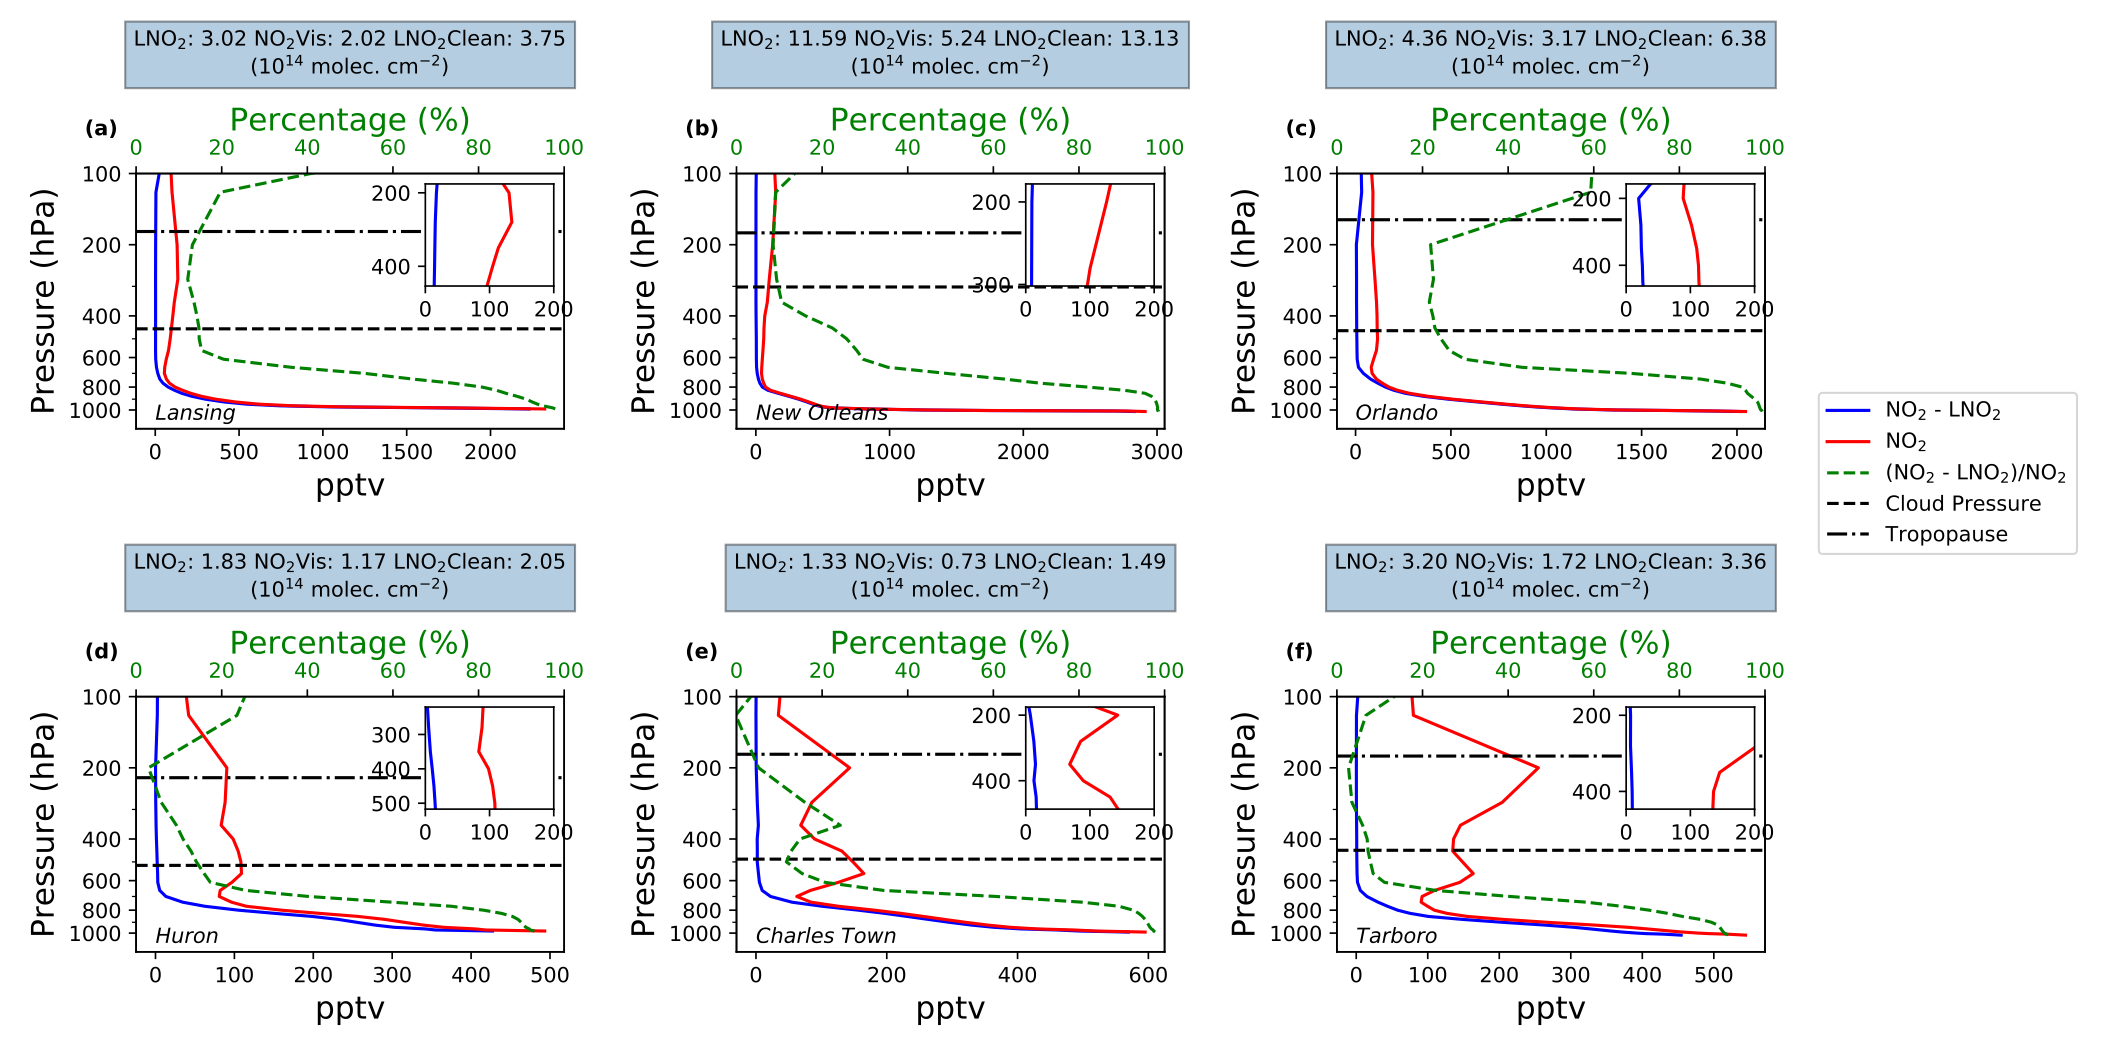
\includegraphics[width=16cm]{./figures/us_bkgd_comp.png}
\caption{在CRF $\geq$ 100\%条件下,六个网格中WRF-Chem 平均NO$_\textrm{2}$ 和背景 NO$_\textrm{2}$ 廓线。
顶行数据选自污染区域(图 \ref{fig:us_delta}a中的星号),而底行数据来自清洁区域(图 \ref{fig:us_delta}a中的三角形)。
绿色虚线是背景 NO$_\textrm{2}$ 与总 NO$_\textrm{2}$ 的平均比例廓线。
放大图显示了从云压到对流层顶的廓线。
标题基于\ref{sec:amf_definition}节定义的三种不同方法估算得到的产量。\\
Figure \ref{fig:us_bkgd_comp}. Comparisons of mean WRF-Chem NO$_\textrm{2}$ and background NO$_\textrm{2}$ profiles in six grids with CRF $\geq$ 100\% on specific days during MJJA 2014.
The top row data are selected from polluted regions (stars in Fig. \ref{fig:us_delta}a) while the bottom row data are from clean regions (triangles in Fig. \ref{fig:us_delta}a).
The green dashed lines are the mean ratio profiles of background NO$_\textrm{2}$ to total NO$_\textrm{2}$.
The zoomed figures show the profiles from the cloud pressure to the tropopause.
The titles present the mean productions based on three different methods mentioned in Sect. \ref{sec:amf_definition}.}
\label{fig:us_bkgd_comp}
\end{figure}


表\ref{table:production_comp}显示了6个城市三种方法之间的相对变化。
AMF$_{\ch{LNO2}}$(式\ref{AMFLNO2_crf100})和 AMF$_{\ch{LNO2Clean}}$(式\ref{AMFLNO2Clean_crf100})之间的区别是分子:
$\int_{p_{\ch{cloud}}}^{p_{\ch{tp}}} w_{\ch{cloudy}}(p) NO_2(p) \: dp$
和$\int_{p_{\ch{cloud}}}^{p_{\ch{tp}}} w_{\ch{cloudy}}(p) LNO_2(p) \: dp$。
当 LNO$_2$ 的比例较高或区域较清洁时,两者相对差异较小(5.0--12.0\%,图\ref{fig:us_bkgd_comp}d--f),
最大的相对差异(46.3\%)发生在对流层上层背景 NO$_2$ 所占比例一直较高的情况下(图\ref{fig:us_bkgd_comp}c)。
因此,我们的方法对背景 NO$_2$ 不太敏感,更适用于受污染地区的对流情况。
相比之下,由于包含了云层下方的 LNO$_2$,我们方法估算的产量大于基于 NO$_2$Vis 的产量。
当云层较高时,特别是 LNO廓线的峰值低于云层时(图\ref{fig:us_bkgd_comp}b),
相对差异较大(121.2\%),因为更多的 LNO$_2$ 不能包含在 NO$_2$Vis 中。
AMF$_{\ch{LNO2Clean}}$(式\ref{AMFLNO2Clean_crf100})和 AMF$_{\ch{NO2Vis}}$(式\ref{AMFNO2Vis_crf100})之间的相对变化取决于
$\int_{p_{\textrm cloud}}^{p_{\textrm tp}} w_{\textrm cloudy}(p) LNO_2(p) \: dp / \int_{p_{\textrm surf}}^{p_{\textrm tp}} w_{\textrm cloudy}(p) LNO_2(p) \: dp$,这也是受云影响,而不是背景NO$_2$。
其中最大的相对变化(153.8\%)发生在新奥尔良,它的云压最小(云层最高),因此可见的柱浓度最小。

图\ref{fig:us_cp_ratio_lno2}a为2014年5--8月在CRF$\geq$90\%的条件下,云压和$V_{\ch{LNO2Vis}}$与$V_{\ch{LNO2}}$之比的日分布。
当云压从600降低到300 hPa时,$V_{\ch{LNO2Vis}}$与$V_{\ch{LNO2}}$之比从 0.8 降低到 0.2,
故在相对清洁的区域,NO$_2$Vis产率小于LNO$_2$产率。
除了 LNO$_2$Vis,LNO$_2$产率也是受云压影响。
对于大于 30 mol每闪击的LNO$_2$产率,云压均小于 550 hPa(图\ref{fig:us_cp_ratio_lno2}b),
而较小的 LNO$_2$ 产率(<30 mol每闪击)出现在 650 和 200 hPa 之间。
由于较高的LNO$_2$ 产率和闪电数据数量有限,现阶段我们无法推出 LNO$_2$ 产率与云压或其他闪电属性之间的关系。
由于云压仅代表云的发展,因此不能仅从云压值推导出闪电的垂直结构。
前人研究表示,闪电通道的长度会有所不同,并且取决于环境条件\citep{Carey.2016,Mecikalski.2017,Fuchs.2018}。
\citet{Davis.2019}比较了两种闪电:正常闪电和异常闪电。
一般来说,正常闪电是上层带正电和中层带负电,而异常闪电则相反\citep{Williams.1989}。
由于异常闪电中上升气流更强且闪电频率更高,因此异常闪电中的对流层上层LNO$_x$浓度高于正常闪电。


\begin{table*}[htbp]
\caption{基于相同先验廓线但不同估算方法时,产量的百分比变化\\Table \ref{table:production_comp}. The percent changes in the estimated production when using different methods based on the same a priori profiles.}
\scriptsize
\begin{tabular}{clccc}
\hline
 & 城市$^a$ & LNO$_2$Clean - LNO$_2$)/LNO$_2$ & LNO$_2$ - TropVis)/TropVis & LNO$_2$Clean-TropVis)/TropVis \\
\hline
\multirow{3}{*}{污染地区} & Lansing          & 24.2\%  & 49.5\%   & 85.6\%   \\
                         & New Orleans      & 13.3\%  & 121.2\%  & 153.8\%  \\
                         & Orlando          & 46.3\%  & 37.5\%   & 101.3\%  \\
\hline
\multirow{3}{*}{清洁地区}    & Huron            & 12.0\%  & 56.4\%   & 75.2\%   \\
                            & Charles Town     & 12.0\%  & 82.2\%   & 104.1\%  \\
                            & Tarboro          & 5.0\%   & 86.0\%   & 95.3\%   \\
\hline
\end{tabular}
\begin{tablenotes}
\footnotesize
\item $^a$城市地址见图\ref{fig:us_delta}a。
\item $^a$Locations are denoted in Fig. \ref{fig:us_delta}a.
\end{tablenotes}
\label{table:production_comp}
\end{table*}

\begin{figure}[H]
\centering
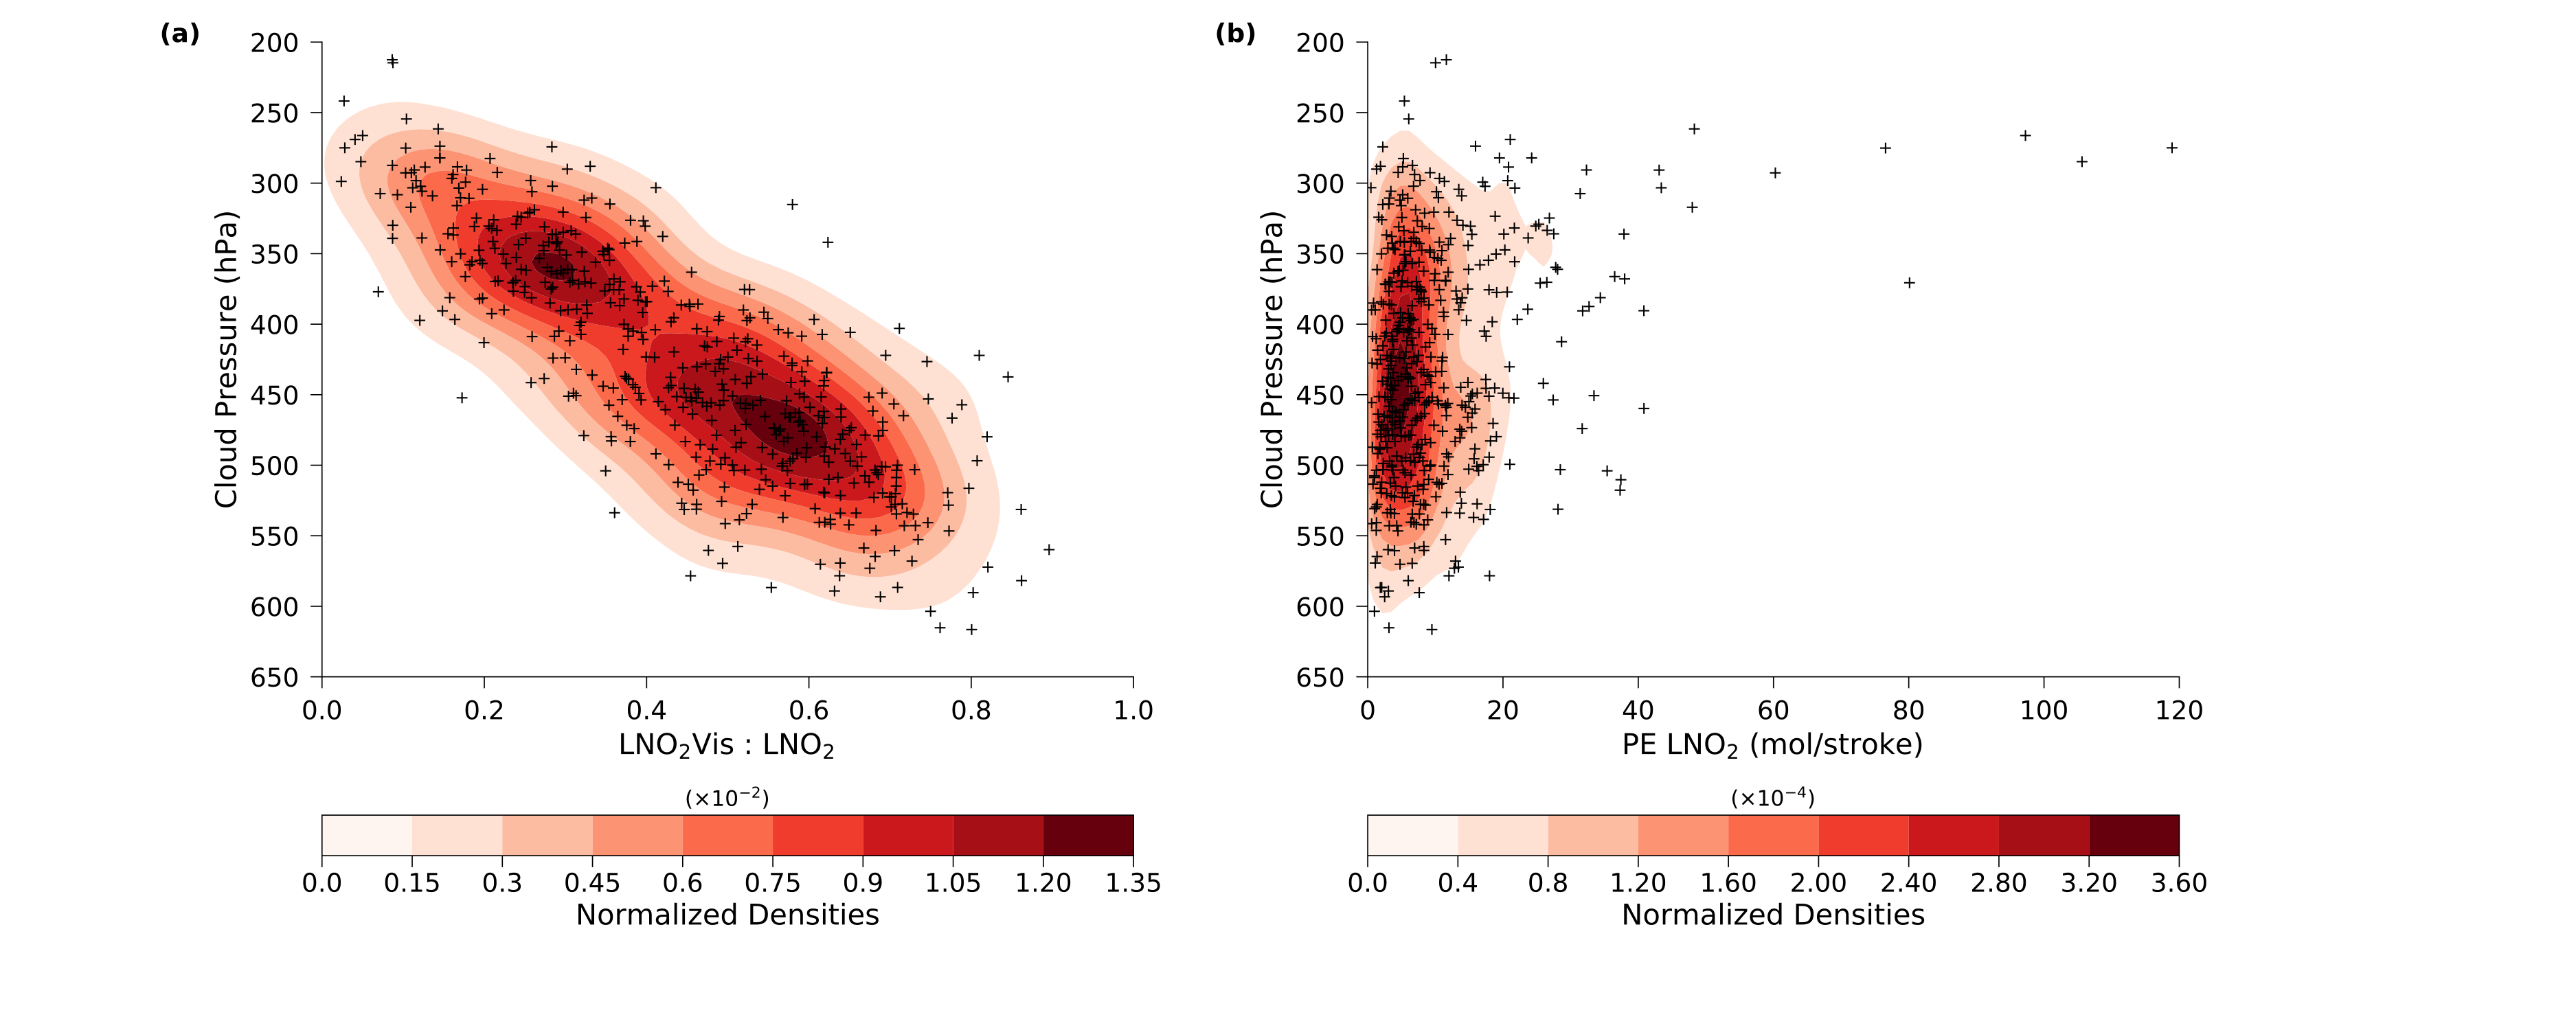
\includegraphics[width=16cm]{./figures/us_cp_ratio_lno2.png}
\caption{(a)$V_{\ch{LNO2Vis}}$与$V_{\ch{LNO2}}$之比的核密度估计;(b)LNO$_2$产率与OMI测得的云压的核密度估计(2014年5--8月,CRF $\geq$ 90\%)。\\
Figure \ref{fig:us_cp_ratio_lno2}. Kernel density estimation of the (a) daily ratio of $V_{\ch{LNO2Vis}}$ to $V_{\ch{LNO2}}$ and (b) daily LNO$_2$ production efficiency (PE) versus the daily cloud pressure measured by OMI with CRF $\geq$ 90\% for MJJA 2014.}
\label{fig:us_cp_ratio_lno2}
\end{figure}


% 模式中LNO$_x$的分布主要有两种方法:已通过对流输送重新分布的LNO$_x$廓线(对流后)和在对流输送重新分布之前LNO$_x$的廓线(对流前)\citep{Allen.2012,Luo.2017}。
% 然而,鉴于与其他 LNO$_x$ 研究相比结果的相似性,我们相信本文研究中基于对流后LNO$_x$廓线的1$^{\circ}$ $\times$ 1$^{\circ}$结果足以估计LNO$_x$的平均产量。
WRF-Chem中LNO排放的设置在不同的研究中有所不同。
\citet{Zhao.2009}在区域尺度模式中将NO$_x$产率设定为250 mol NO每闪电,
而 \citet{Bela.2016}选择了\citet{Barth.2012}使用的330 mol NO每闪电。
\citet{Wang.2015a}假设每次闪电产生大约 500 mol NO,这是通过云尺度化学传输模式和云中飞机观测得出的\citep{Ott.2010}。
为了评估 LNO$_x$参数化对 LNO$_x$估算的影响,
我们将基于另一个LNO设置(2$\times$基本闪率,500 mol NO每闪电,以下简称“2$\times$500 mol NO每闪电”)的WRF-Chem结果中NO$_2$廓线
应用于先验廓线并评估 AMF$_{\ch{LNO$_2$}}$、AMF$_{\ch{LNO$_x$}}$、LNO$_2$产率和 LNO$_x$产率的变化。
对于线性回归方法(图 \ref{fig:us_pe_linear_2x500}),LNO$_2$产率为 29.8 $\pm$ 20.5 mol每闪电,
比基本方法(18.7 $\pm$ 18.1 mol每闪电)大59.4\%。
同时,LNO$_x$产率(从54.5 $\pm$ 48.1 mol每闪电增加到88.5 $\pm$ 61.1 mol每闪电)也取决于 WRF-Chem 中 LNO产率的设置。
通过比较图\ref{fig:us_pe_linear}和图\ref{fig:us_pe_linear_2x500},我们发现当LNO$_2$和NO$_2$Vis产率呈现相同趋势时,
LNO$_2$Clean和 LNO$_2$产率更相似。
目前尚不清楚 NO--NO$_2$--O$_3$ 循环或其他 LNO$_x$ 汇对LNO$_x$产率变化的贡献。
这需利用 WRF-Chem进行详细的来源解析,超出了目前本研究的范围。

\begin{figure}[H]
\centering
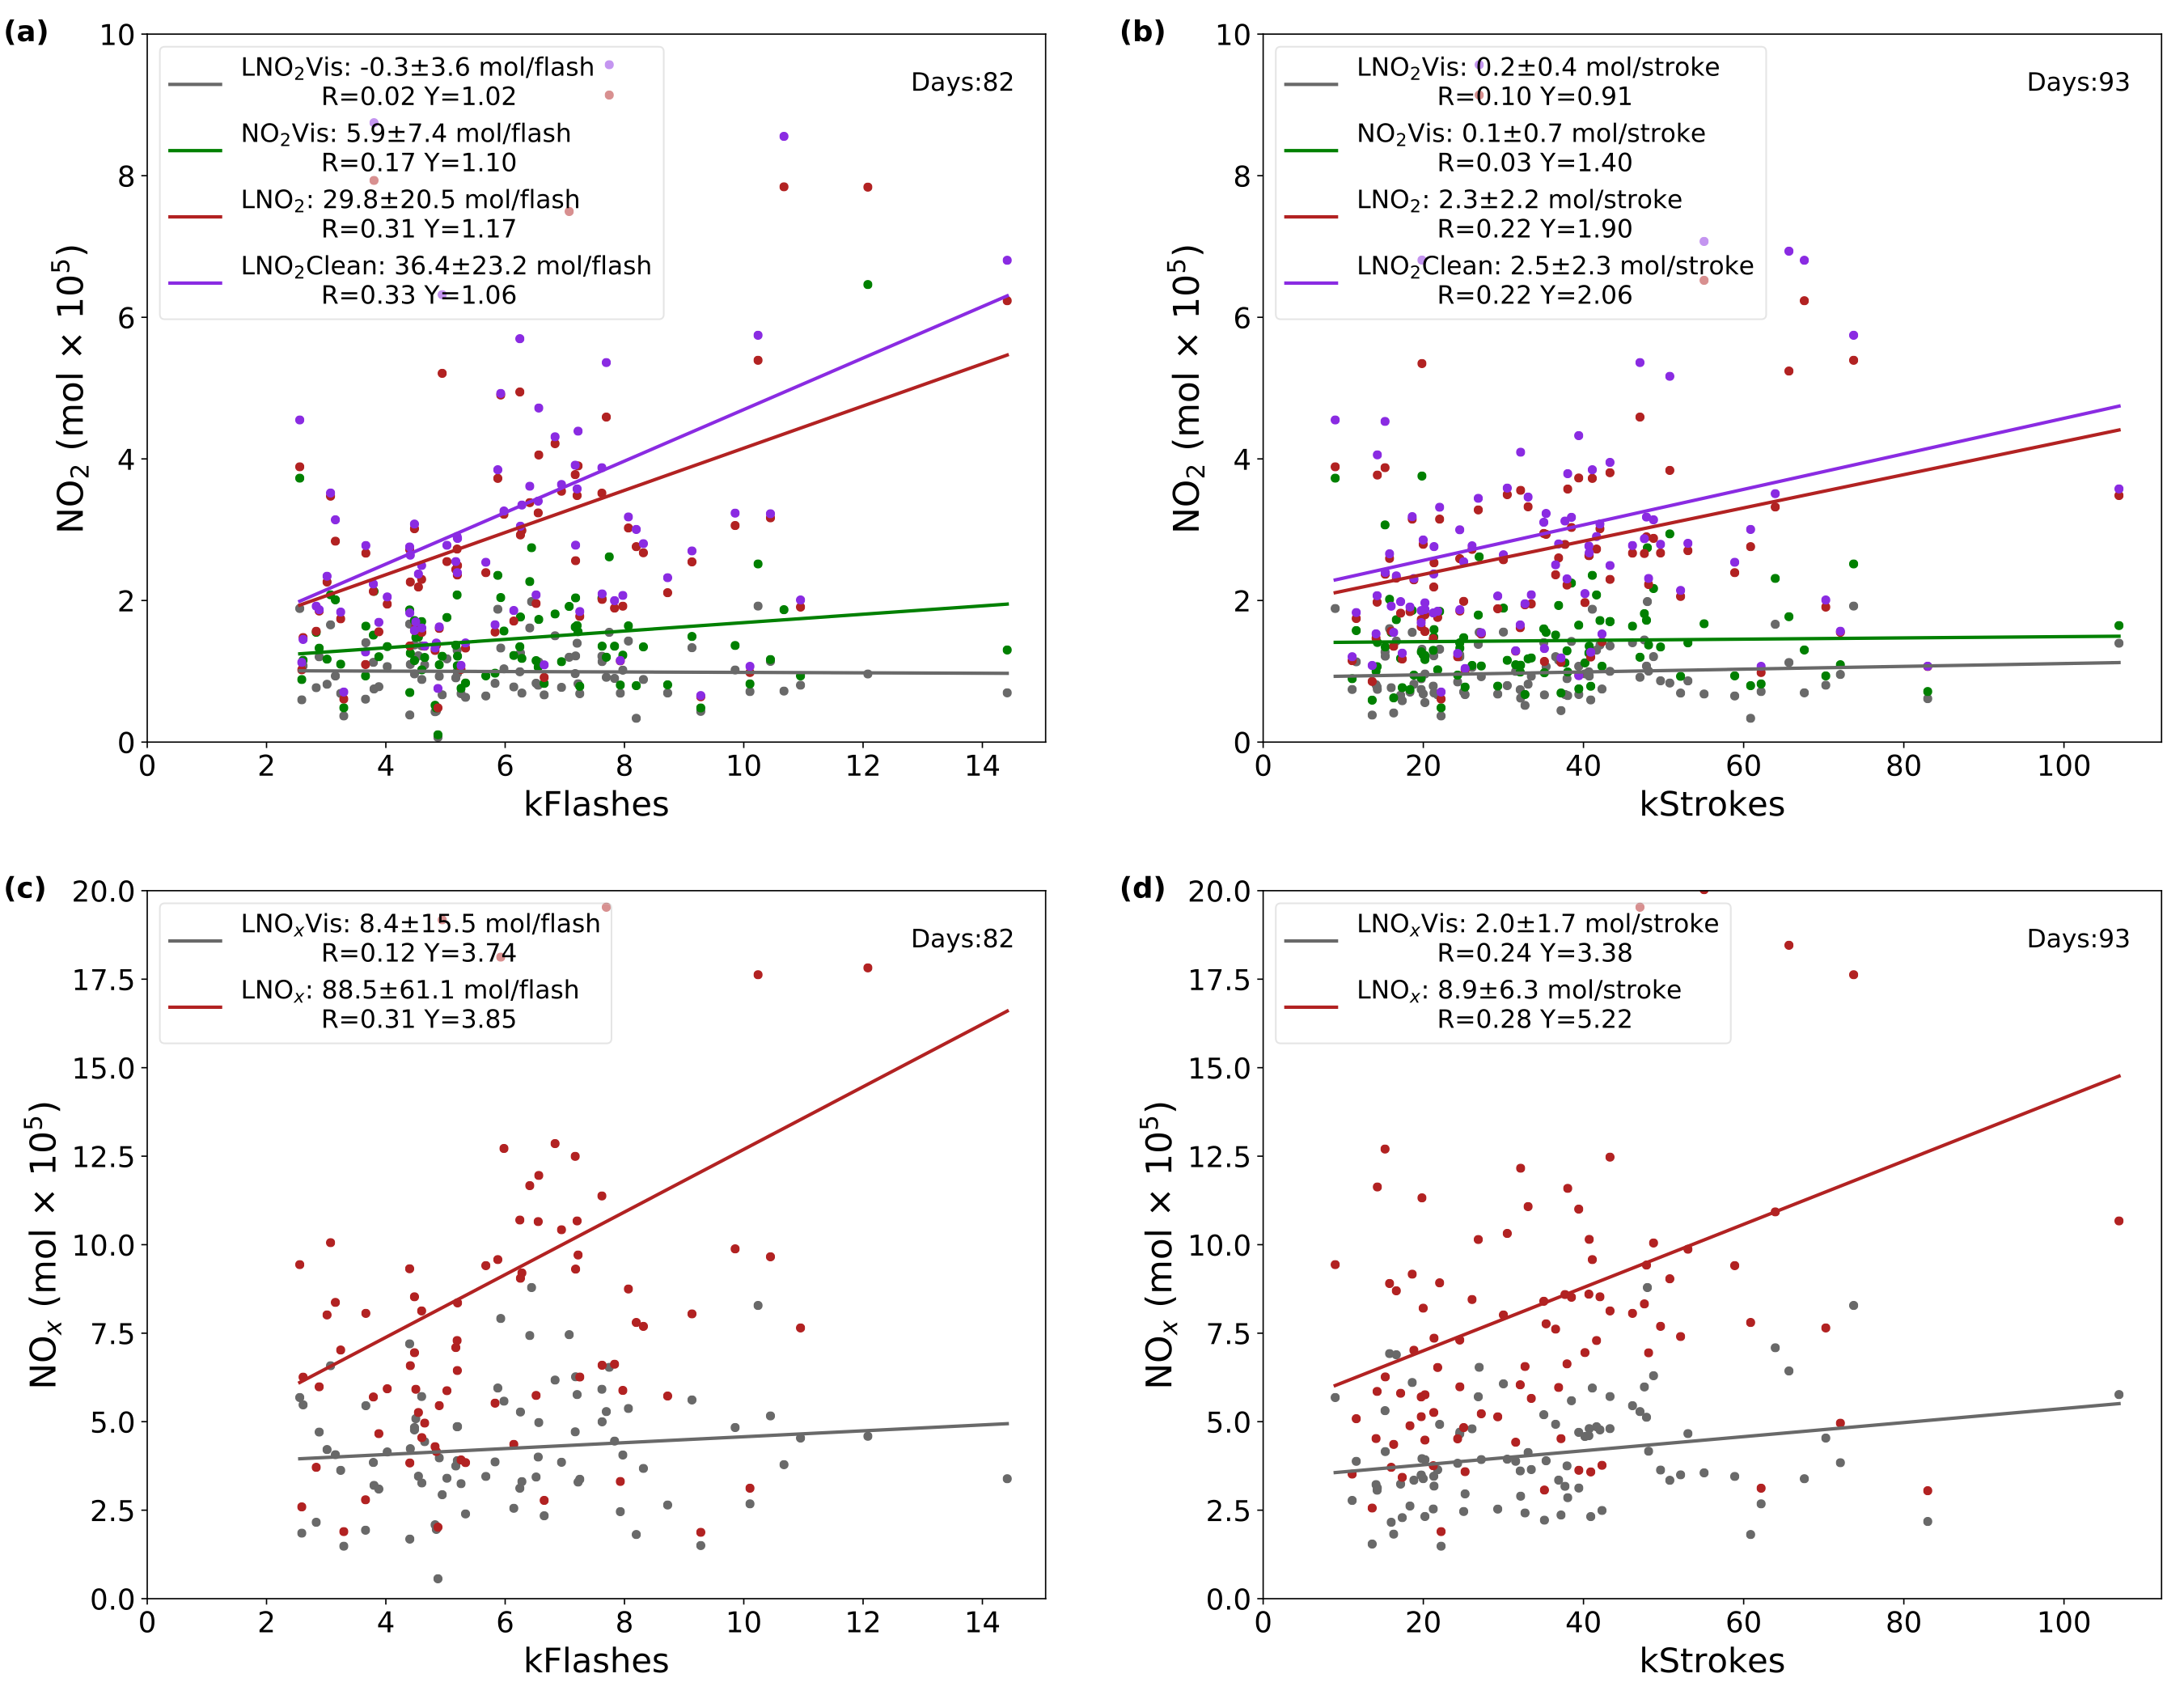
\includegraphics[width=13cm]{./figures/us_pe_linear_2x500.png}
\caption{与图\ref{fig:us_pe_linear}相同,但是模式中NO产率设置为2$\times$500 mol每闪电 \\Figure \ref{fig:us_pe_linear_2x500}. Same as Fig. \ref{fig:us_pe_linear} except for the 2$\times$500 mol NO flash$^{-1}$ configuration.}
\label{fig:us_pe_linear_2x500}
\end{figure}

图\ref{fig:us_simulation_diff}显示了基于 1$\times$200 和 2$\times$500 mol NO 每闪电得到的AMF$_\textrm{LNO$_2$}$、AMF$_\textrm{LNO$_x$}$、LNO$_2$和 LNO$_x$ 的平均百分比变化。
更高的LNO产率设置对LNO$_2$和 LNO$_x$的影响趋势相同:较小的AMF$_\textrm{LNO$_2$}$和AMF$_\textrm{LNO$_x$}$导致较大的LNO$_2$和 LNO$_x$,但变化幅度具有区域性。
这是由AMF$_\textrm{LNO$_2$}$和AMF$_\textrm{LNO$_x$}$的非线性计算引起的。
随着LNO$_2$的贡献增大,AMF方程式的分子和分母都增大。
因为LNO$_2$只占云上NO$_2$的一小部分,分母增加的幅度可能与分子增加的幅度不同,从而对AMF$_\textrm{LNO$_2$}$和AMF$_\textrm{LNO$_x$}$产生不同的影响。
如\citet{Zhu.2019}所述,使用 2$\times$500 mol NO 每闪电的设置和与我们相同的闪电参数化可能会高估美国东南部的闪电密度。
幸运的是,该地区的 AMF 和估算得到的LNO$_2$变化不大。
由于美国东南部的闪电密度最高,因此 AMF 分子中的NO$_2$以LNO$_2$为主。
当模式使用较高的LNO$_2$时,分子和分母增幅相当。
换言之,对 LNO 设置的敏感性降低,LNO$_2$的相对分布很重要。

\begin{figure}[H]
\centering
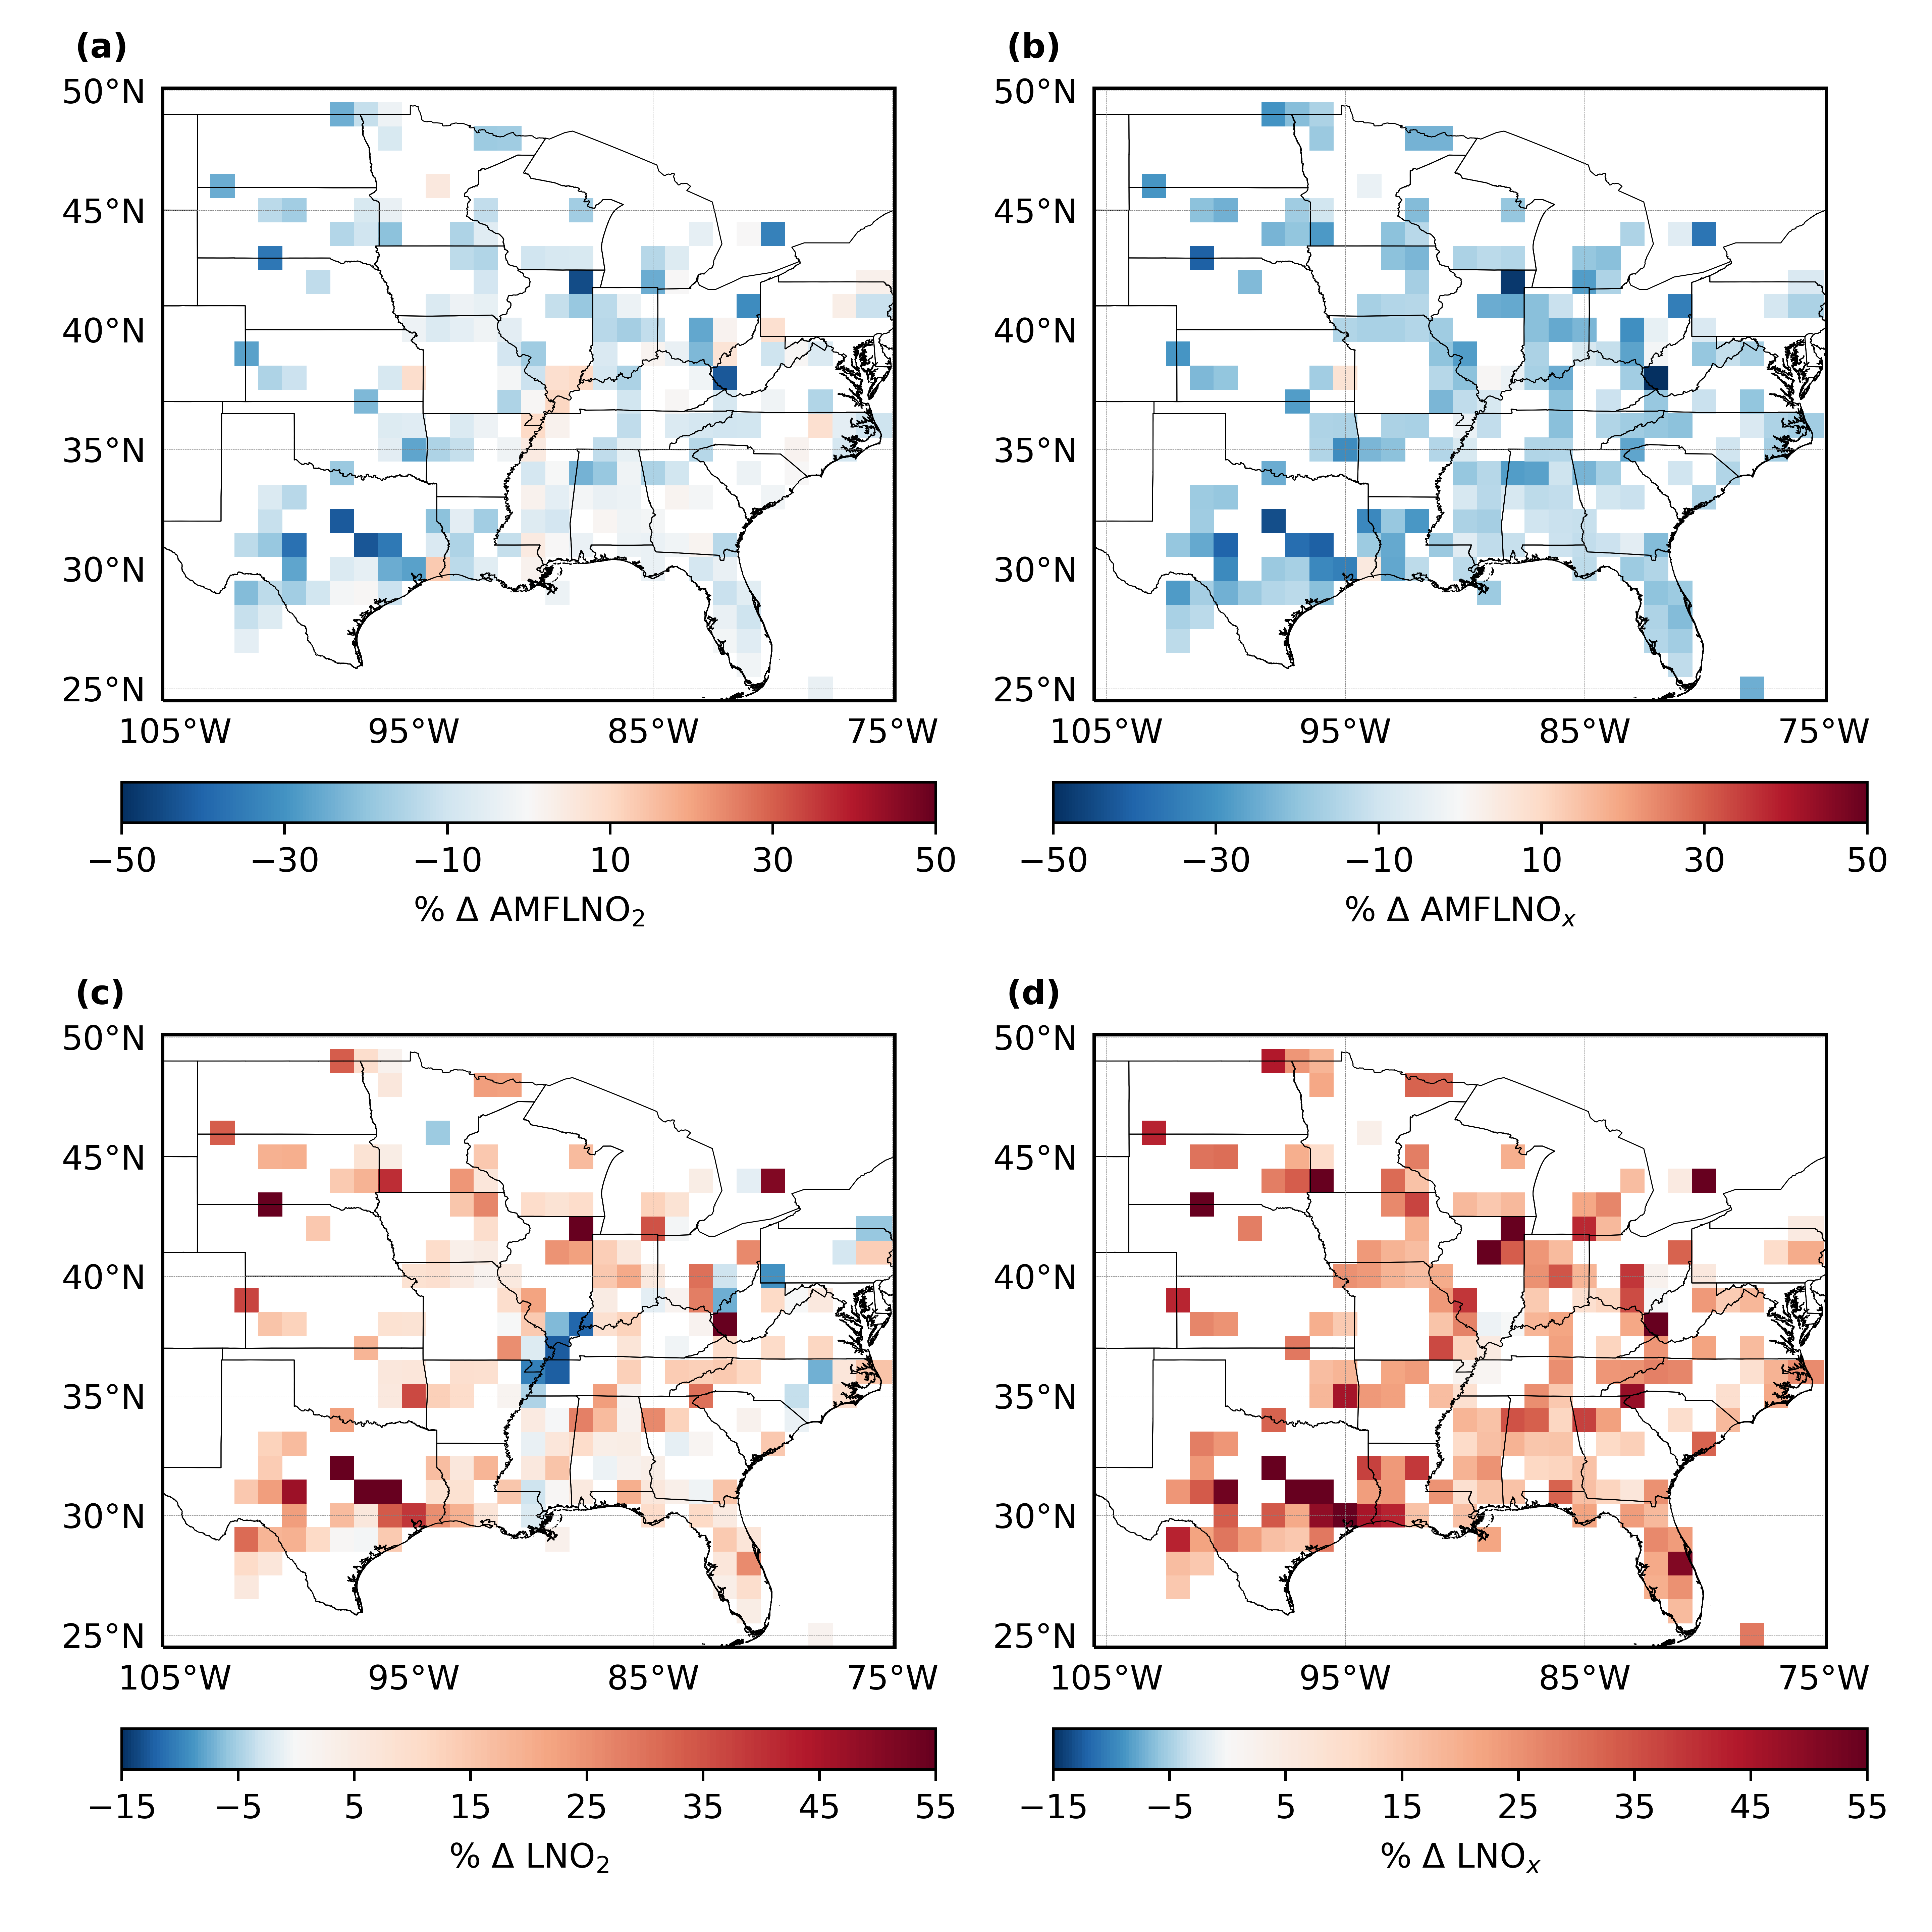
\includegraphics[width=13cm]{./figures/us_simulation_diff.png}
\caption{2014年5--8月在CRF $\geq$ 90\% 条件下,
(a)AMF$_{\textrm{LNO$_2$}}$;(b)AMF$_{\textrm{LNO$_x$}}$;
(c)LNO$_\textrm{2}$ 和 (d) LNO$_\textrm{x}$的平均百分比差异。
廓线之间的差异为 2$\times$500 mol NO每闪电 和 1$\times$200 mol NO每闪电所得结果之差。\\
Figure \ref{fig:us_simulation_diff}. Average percent differences in (a) AMF$_{\textrm{LNO$_2$}}$, (b) AMF$_{\textrm{LNO$_x$}}$, (c) LNO$_\textrm{2}$ and (d) LNO$_\textrm{x}$ with CRF $\geq$ 90\% over MJJA 2014.
Differences between profiles are generated by 2$\times$500 mol NO flash$^{-1}$ and 1$\times$200 mol NO flash$^{-1}$.}
\label{fig:us_simulation_diff}
\end{figure}

图\ref{fig:us_lno2_profile}显示了两个特定区域的平均 LNO 和 LNO$_2$ 曲线的比较,
其中 2$\times$500 mol NO 每闪电设置分别导致两区域较低和较高的 LNO$_2$产率。
第一个所选区域(36--37$^{\circ}$ N,89--90$^{\circ}$ W,图\ref{fig:us_lno2_profile}a)是 LNO$_2$ 负百分比变化最小的区域(图\ref{fig:us_simulation_diff}c)。
第二个所选区域(31--32$^{\circ}$ N,97--98$^{\circ}$ W,图\ref{fig:us_lno2_profile}b)是LNO$_2$ 正百分比变化最大的区域(图\ref{fig:us_simulation_diff}c)。
尽管两个区域的平均 LNO 和 LNO$_2$廓线的相对分布相似,但量级相差10 倍。
这意味着 WRF-Chem中闪电参数化的表现具有区域性,并且对流层上层可能会出现不切实际的廓线。
虽然这种敏感性分析在某些地区是错误的,但它可得到由于 LNO 和 LNO$_2$ 廓线而影响NO$_2$的上限。
正如\citet{Laughner.2017}中所讨论的,在多云条件下散射权重是均匀的,并且由于高反照率,NO$_2$ 的灵敏度在不同高度上几乎是恒定的。
但是,我们应仔细考虑对流层上层LNO$_2$ 的相对分布。
如果云层上方的 LNO$_2$ ∕ NO$_2$ 足够大(图\ref{fig:us_lno2_profile}a),
AMF$_{\ch{LNO2}}$ 很大程度上取决于 LNO$_2$Vis 与 LNO$_2$ 的比值,
这与相对分布有关。
当不满足高 LNO$_2$ ∕ NO$_2$ 的条件时,相对分布和比例都很重要(图\ref{fig:us_lno2_profile}b)。

为了说明这一点,我们使用了不同的LNO产率设置来对LNO$_2$、LNO$_2$Vis、LNO$_2$Clean 和 NO$_2$Vis进行敏感性试验(图\ref{fig:us_lno2_profile})。
其中CRF 的阈值设置为 100\% 以简化等式。
总体上来说,LNO$_2$Clean 和 NO$_2$Vis 的差异小于 LNO$_2$ 和 LNO$_2$Vis 的差异。
通过比较方程中的分子和分母,可得知为何不同的LNO排放设置产生的影响在图\ref{fig:us_lno2_profile}c和d中较小。
对于 LNO$_2$Clean 和 NO$_2$Vis,当更多(更少)LNO$_2$ 或 NO$_2$ 存在时,S$_{\ch{NO2}}$ 和 V$_{\ch{NO2}}$ 都会增加(减少)。
图\ref{fig:us_lno2_profile}a和b的区别是分母,分别为总对流层 LNO$_2$ 垂直柱浓度和可见 LNO$_2$ 垂直柱浓度。
因此,图\ref{fig:us_lno2_profile}a中的负值是由云下的 LNO$_2$ 部分引起的。
故该误差可导致LNO$_2$ 和 LNO$_x$产率的不确定性,我们保守估计这分别为 $\pm$13\% 和 $\pm$25\%。
最终LNO$_2$ 和 LNO$_x$产率的不确定性是根据\citet{Pickering.2016,Allen.2019,Bucsela.2019,Lapierre.2020}的方法得到,即通过依次扰动每个参数来重新计算LNO$_2$ 和 LNO$_x$从而得到不确定性(表\ref{table:us_uncertainty})。


\begin{figure}[H]
\centering
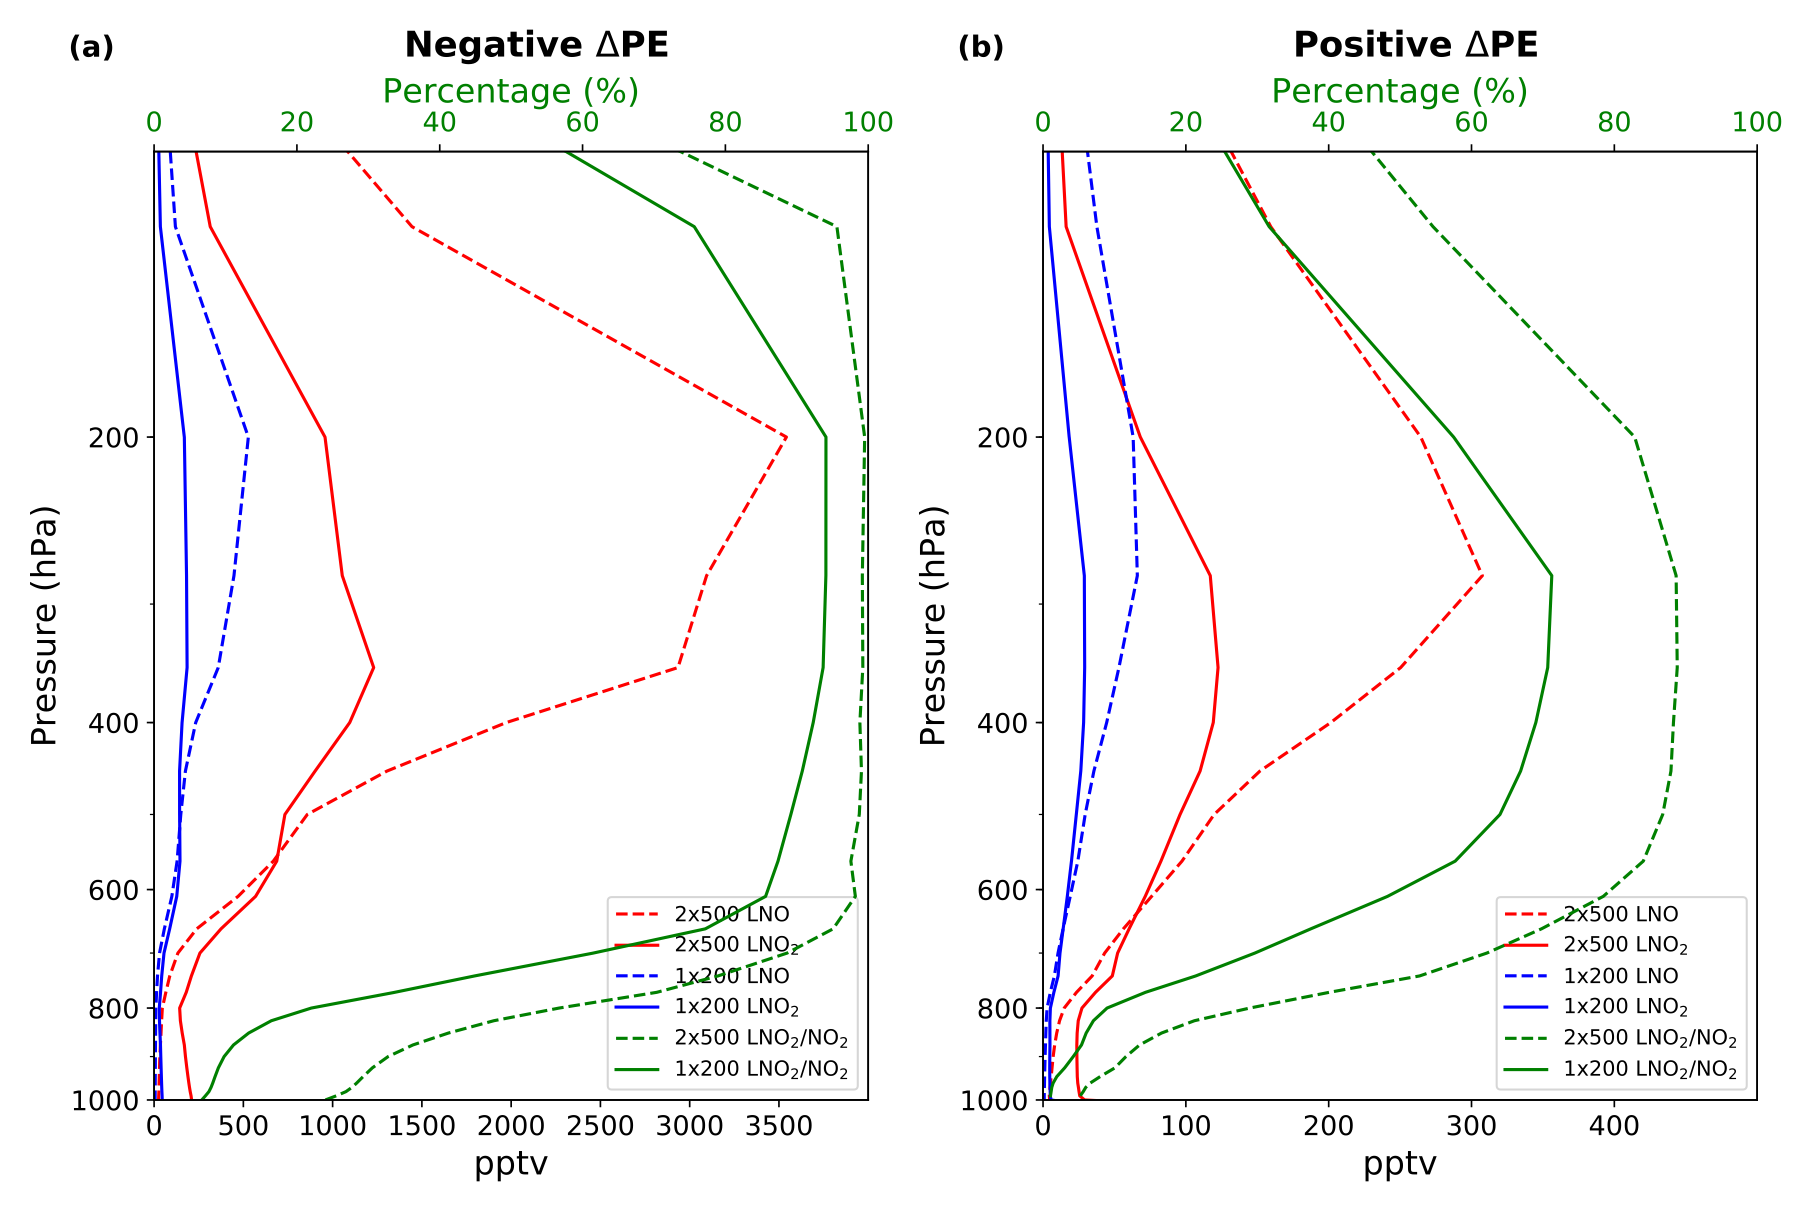
\includegraphics[width=13cm]{./figures/us_lno2_profile.png}
\caption{当LNO 设置从 1$\times$200 mol NO每闪电 更改为 2$\times$500 mol NO每闪电 时,
(a)包含 LNO$_2$ 的最小负百分比变化的区域和(b)包含最大正百分比变化的区域中LNO 和 LNO$_2$ 的平均廓线廓线。
使用 1$\times$200(2$\times$500)mol NO每闪电的曲线以蓝色(红色)线显示。
绿色实线(虚线)是 在1$\times$200(2$\times$500)mol NO每闪电设置下,LNO$_2$ 与 NO$_2$ 的平均比例。\\
Figure \ref{fig:us_lno2_profile}. LNO and LNO$_2$ profiles with different LNO settings at (a) the region containing the minimal negative percent change in LNO$_2$ and (b) the region containing the largest positive percent change in LNO$_2$ when the LNO setting is changed from 1$\times$200 mol NO flash$^{-1}$ to 2$\times$500 mol NO flash$^{-1}$, averaged over MJJA 2014.
The profiles using 1$\times$200 (2$\times$500) mol NO flash$^{-1}$ are shown in blue (red) lines.
Solid (dashed) green lines are the mean ratio of LNO$_2$ to NO$_2$ with 1$\times$200 (2$\times$500) mol NO flash$^{-1}$.}
\label{fig:us_lno2_profile}
\end{figure}


我们使用与 NASA 标准产品一致的 GEOS-5 月平均对流层顶气压,而不是可变的 WRF 对流层顶高度来评估由 BEHR 对流层顶压造成的不确定性。
\citet{Acarreta.2004}等人将云压偏差用云压和云分数的函数表示,依此我们得到计算的LNO$_2$产率不确定性为 32\%,
LNO$_x$产率不确定性为 34\%,这是估算中最大的不确定性来源。
接着,由于GLOBE地形高度数据的分辨率远高于OMI像素,在BEHR算法中采用假设的固定比例高度。
因此,\citet{Laughner.2019a}将 WRF 平均表面气压与 GLOBE 表面气压进行了比较,得出最大偏差为 1.5\%。
基于最大偏差,我们改变了地表气压并限制其小于 1020 hPa,得到的不确定性可忽略不计。

云辐射分数的误差可由云分数得到

\begin{equation}
\sigma = 0.05 \times \left.\frac{\partial{f_r}}{\partial{f_g}}\right|_{f_{g,pix}}
\end{equation}

其中 $f_r$ 是云辐射度分数,$f_g$ 是云分数,$f_{g,pix}$ 是特定像素的云分数。
对于 LNO$_2$ 和 LNO$_x$产率,云分数的误差转换为 2\% 的云辐射分数误差。

500m MODIS 反照率产品的精度通常在站点反照率观测值的 5\% 以内,而那些低质量的异常值主要在观测数据的 10\% 以内\citep{Schaaf.2011}。
由于我们直接使用双向反射率分布函数(BRDF)数据,而不包含辐射传输模型,
因此将 14\% 的朗伯等效反射率误差和 10\% 的不确定性结合起来得到 17\% 的扰动\citep{Laughner.2019a},重新计算结果显示该扰动对于估算的影响也可忽略。

与 NASA 标准产品 v2 相比,\citet{Krotkov.2017}证明V$_\textrm{strat}$中的误差为 10$^{14}$ cm$^{-2}$。
在污染区域该误差可能略大于此值,而在最清洁区域的误差通常要小得多\citep{Bucsela.2013}。
依据\citet{Allen.2019},我们估计V$_\textrm{strat}$分量的不确定性和斜柱误差分别为 10\% 和 5\%。

基于美国大陆上相对于 LIS 的检测效率,ENTLN 检测效率的不确定性对于云闪为 $\pm$ 16\%,
由于地闪 在美国大陆具有高检测效率,不确定性估计为 $\pm$ 5\% \citep{Lapierre.2020},由此产生的估算不确定度为15\%。
此外,我们使用 2.4 h 的时间窗口中的ENTLN闪电和闪击来分析 NO$_2$ 和 LNO$_x$ 的产率。
由于从 ERA5 再分析得出的时间窗口不能代表可变风速,因此进行了敏感性试验。
使用 2 和 4 h 的时间窗口得出闪电产量的不确定性为 10\%,闪击产量的不确定性为 8\%。
此外,对流层上层NO$_x$ 的寿命范围为 2--12 h,具体取决于对流位置、过氧硝酸甲酯、烷基以及多功能硝酸盐\citep{Nault.2017}。
我们将方程式中的6 h用 2 和 12 h 代替,从而得到由于寿命导致的不确定性为 24\%,
这与 LNO$_x$ 类型的闪电参数化引起的不确定性(25\%)相当。

最近的研究表明,模拟的 NO ∕ NO$_2$比例与 SEAC4RS 飞机观测的数据不同\citep{Travis.2016,Silvern.2018}。
\citet{Silvern.2018}将此归因于对 NO$_2$ 测量的正干扰或低温 NO--NO$_2$--O$_3$ 光化学反应速率的误差。
考虑到可能的 NO$_2$ 测量正干扰\citep{Allen.2019,Bucsela.2019},
我们为该误差分配 20\% 偏差和 $\pm$ 15\% 不确定性,并估计产率的不确定性为 15\%。

此外,LNO$_x$产率的估算还取决于对流层背景NO$_2$浓度。
在我们的方法中,影响该因素的主要因素是排放清单和传输的 NO$_2$。
对于排放清单,不确定性的来源是假设条件、计算方法、输入数据和计算误差。
因此,与 NO$_2$ 相关的不同物种或污染物的不确定性是不同的,美国环保署也没有公布量化的不确定性数据。
对于模拟的对流传输,\citet{Li.2018}将云解析模拟与基于对流参数化的模拟进行了比较,并指出对流输送在参数化中较弱。
但是,我们认为比例条件(LNO$_2$Vis/NO$_2$Vis $\geq$ 50\%)应该减少了这两种不确定性,
我们假设背景NO$_2$浓度导致的不确定性为 10\%,小于 \citet{Allen.2019}和\citet{Bucsela.2019}等研究中使用的 20\%。

净不确定性为表\ref{table:us_uncertainty}中所有单个不确定性平方和的平方根。
LNO$_2$ 类型和 LNO$_x$ 类型的净不确定性分别为 48\% 和 56\%。
基于线性回归和求和法的平均结果为32 mol NO$_2$每闪电、90 mol NO$_x$每闪电、6 mol NO$_2$每闪击 和 17 mol NO$_x$每闪击。
将相应的不确定性应用于这些平均值,我们得出32 $\pm$ 15 mol NO$_2$每闪电、90 $\pm$ 50 mol NO$_x$每闪电、
6 $\pm$ 3 mol NO$_2$每闪击 和17 $\pm$ 10 mol NO$_x$每闪击。
这在当前文献估计(33--500 mol NO$_x$每闪电)的范围内\citep{Schumann.2007,Beirle.2010,Bucsela.2010}。
最近\citet{Bucsela.2010}研究中估算的LNO$_x$产率为 100--250 mol NO$_x$每闪电,高于但与我们的估计结果相重叠。
\citet{Pickering.2016}估算的墨西哥湾LNO$_x$产率为 80 $\pm$ 45 mol NO$_x$每闪电,比本研究中美国大陆的结果低50\%。
因为墨西哥湾上空有很多许多缺失数据,因此两个研究实际上是不同地区之间的比较。
如果\citet{Pickering.2016}的方法未对背景NO$_2$进行校正,得出的 LNO$_x$产率在清洁区域或云上LNO$_2$浓度高的区域与我们的相似,但在污染区域可能高估18\%以上。
对于基于闪击的结果,\citet{Lapierre.2020}得到的LNO$_2$产率较低,为1.6 $\pm$ 0.1 mol NO$_2$每闪击。
该差异是由不同版本的 BEHR 算法和其他设置引起的,由于我们的方法将云下LNO$_2$考虑进总的LNO$_2$,所以得到的LNO$_2$产量可能会更大,尤其是对于高的云层。



\begin{table*}[H]
\centering
\caption{估算LNO$_2$和LNO$_x$产率的不确定性\\ Table \ref{table:us_uncertainty}. Uncertainties for the estimation of LNO$_2$ and LNO$_x$ production efficiencies (PE).}
\scriptsize
\begin{tabular}{llllll}
\hline
来源 & 扰动 & NO$_2$每闪电$^e$ & NO$_x$每闪电$^e$ & NO$_2$每闪击$^e$ & NO$_x$每闪击$^e$ \\
\hline
BEHR对流层顶高度$^a$                    & NASA产品                              & 6   & 4   & 6   & 4 \\
云辐射分数$^a$                          & $\pm$ 5\%                            & 2   & 2   & 2   & 2 \\
云压$^b$                               & 变化的                                & 32  & 34  & 32  & 34 \\
地表气压$^a$                            & $\pm$ 1.5\%                          & 0   & 0   & 0   & 0 \\
地表反照率$^a$                          & $\pm$ 17\%                           & 0   & 0   & 0   & 0 \\
LNO$_2$廓线$^a$               & 2$\times$500 mol NO每闪电             & 13  & 25  & 13  & 25 \\
廓线位置$^a$                            & 拟蒙特卡罗法                           & 0   & 1   & 0   & 1 \\
闪电探测效率$^c$                        & 云闪: $\pm$ 16\%, 地闪: $\pm$ 5\%        & 15  & 15  & 15  & 15 \\
时间窗口%
$^c$                                  & 2 -- 4 hours                         & 10  & 10  & 8   & 8 \\
LNO$_x$寿命%
$^c$                                  & 2 -- 12 hours                        & 24  & 24  & 24  & 24 \\
V$_{strat}$%
$^d$                                  & -                                    & 10  & 10  & 10  & 10 \\
斜柱浓度的系统误差$^d$                   & -                                    & 5   & 5   & 5   & 5 \\
对流层背景浓度$^d$           & -                                    & 10  & 10  & 10  & 10  \\
NO/NO$_2$%
$^d$                                  & 20\% $\pm$ 15\%                      & 0   & 15  & 0   & 15 \\
净                                   & -                                    & 49  & 56  & 48  & 56 \\
\hline
\end{tabular}
\begin{tablenotes}
\footnotesize
\item PE$_{\ch{不确定性}}$ = (误差$_{\ch{高扰动值}}$ - 误差$_{\ch{低扰动值}}$)/2,
其中 误差$_{\ch{\* 扰动值}}$ = (PE$_{\ch{\* 扰动值}}$ - PE$_{\ch{原始值}}$)/PE$_{\ch{原始值}}$。
\item PE$_{\ch{uncertainty}}$ = (Error$_{\ch{rising\ perturbed\ value}}$ - Error$_{\ch{lowering\ perturbed\ value}}$)/2
where Error$_{\ch{\* perturbed value}}$ = (PE$_{\ch{\* perturbed\ value}}$ - PE$_{\ch{original\ value}}$)/PE$_{\ch{original\ value}}$.
\item $^a$ \citet{Laughner.2019a}, $^b$ \citet{Acarreta.2004}, $^c$ \citet{Lapierre.2020}, $^d$ \citet{Allen.2019} and\ \citet{Bucsela.2019}, $^e$ Uncertainty (\%)
\end{tablenotes}
\label{table:us_uncertainty}
\end{table*}

\section{污染地区(中国东南部)} \label{sec:china}

\subsection{模式设置} \label{sec:model_settings_china}

中国东南部的研究使用的WRF-Chem版本号为4.1.4,气象条件的初始场和边界场来自1小时分辨率的欧洲中心大气再分析数据[ERA5,\citet{Hersbach.2020}]。
模式的垂直分层为75层,对流层顶设置为50 hPa,嵌套区域如图\ref{fig:domains_china}所示。
微物理过程使用WSM6方案\citep{Hong.2006a},而短波和长波辐射使用RRTMG方案\citep{Iacono.2008},陆面过程由Noah方案模拟\citep{Koren.1999}。
但是,我们使用不同的边界层参数化来模拟两次对流个例,2019年的个例使用YSU方案\citep{Hong.2006},而2020年的个例使用QNSE方案\citep{Sukoriansky.2005}。

化学初始场和边界场采用整个大气社区气候模式(WACCM,\url{https://www.acom.ucar.edu/waccm/})的输出数据。
其中2020年个例的初始O$_3$廓线使用臭氧探空仪观测所得的O$_3$廓线。
人为排放使用2016年中国多分辨率排放清单(MEIC,\url{http://www.meicmodel.org/})1.3版驱动,
生物排放采用来自自然界的气体和气溶胶排放模型[MEGAN,\citet{Guenther.2006}]。
化学方案使用气相化学的臭氧和相关化学示踪剂模式(MOZART)和气溶胶的Goddard化学气溶胶辐射和传输(GOCART)模式\citep{Pfister.2011}。
其中光解方案采用基于云光学厚度(cloud\_fraction$^{1.5}$)的新对流层紫外线和可见光(TUV)方案,即光解速率依赖于气溶胶和云。
此外LNO的垂直廓线使用\citet{Ott.2010}的双峰型LNO廓线\citep{Laughner.2017},而LNO和LNO$_2$廓线是指开启和关闭LNO排放的模拟垂直廓线的差异,
其中LNO$_x$参数化调整为每次闪电产生500 mol NO\citep{Zhu.2019}。

\begin{figure}[H]
\centering
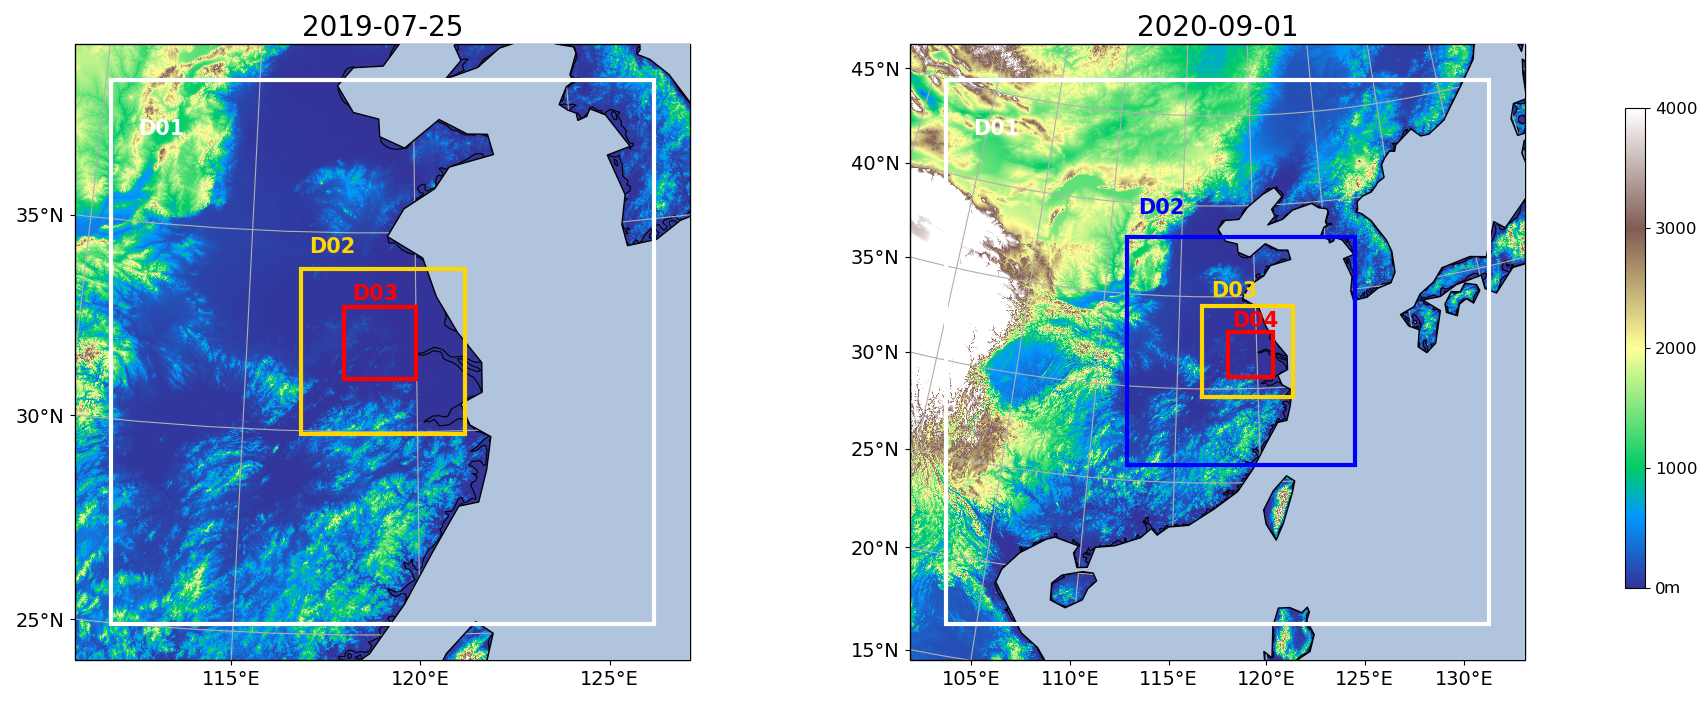
\includegraphics[width=0.9\textwidth]{./figures/domains_china.png}
\caption{2019年和2020年个例的WRF-Chem模拟区域和地形高度(m)图。
2019年个例的水平网格分辨率为15 km(D01)、3 km(D02)和 0.6 km(D03)。
对于2020年个例,分别为27 km(D01)、9 km(D02)、3 km(D03)和 1 km(D04)。\\
Figure \ref{fig:domains_china}. Domain and terrain height (m) of the WRF-Chem simulations for the 2019 and 2020 cases. The horizontal grid resolution of
domains for the 2019 case is 15 km (D01), 3 km (D02) and 0.6 km (D03). For the 2020 case, it is 27 km (D01), 9 km (D02), 3 km (D03),
and 1 km (D04).}
\label{fig:domains_china}
\end{figure}

% \subsection{闪电氮氧化物的反演} \label{subsec:retrieval_china}
\subsection{闪电氮氧化物的产率}

图\ref{fig:china_flash_scd}a--d将对流层NO$_2$斜柱浓度($S_{\ch{NO2}}$)的分布与观测的闪电分布进行了比较。
尽管由于探测器饱和和光晕效应,闪电最活跃像素上的$S_{\ch{NO2}}$无效,但对流附近或出流区仍有有效数据。
在2019年的个例中,闪电发生在TROPOMI过境前不到30分钟,
但2020年的个例中既有新生的也有老化的LNO$_2$(图\ref{fig:china_flash_scd}d)。

\begin{figure}[H]
    \centering
    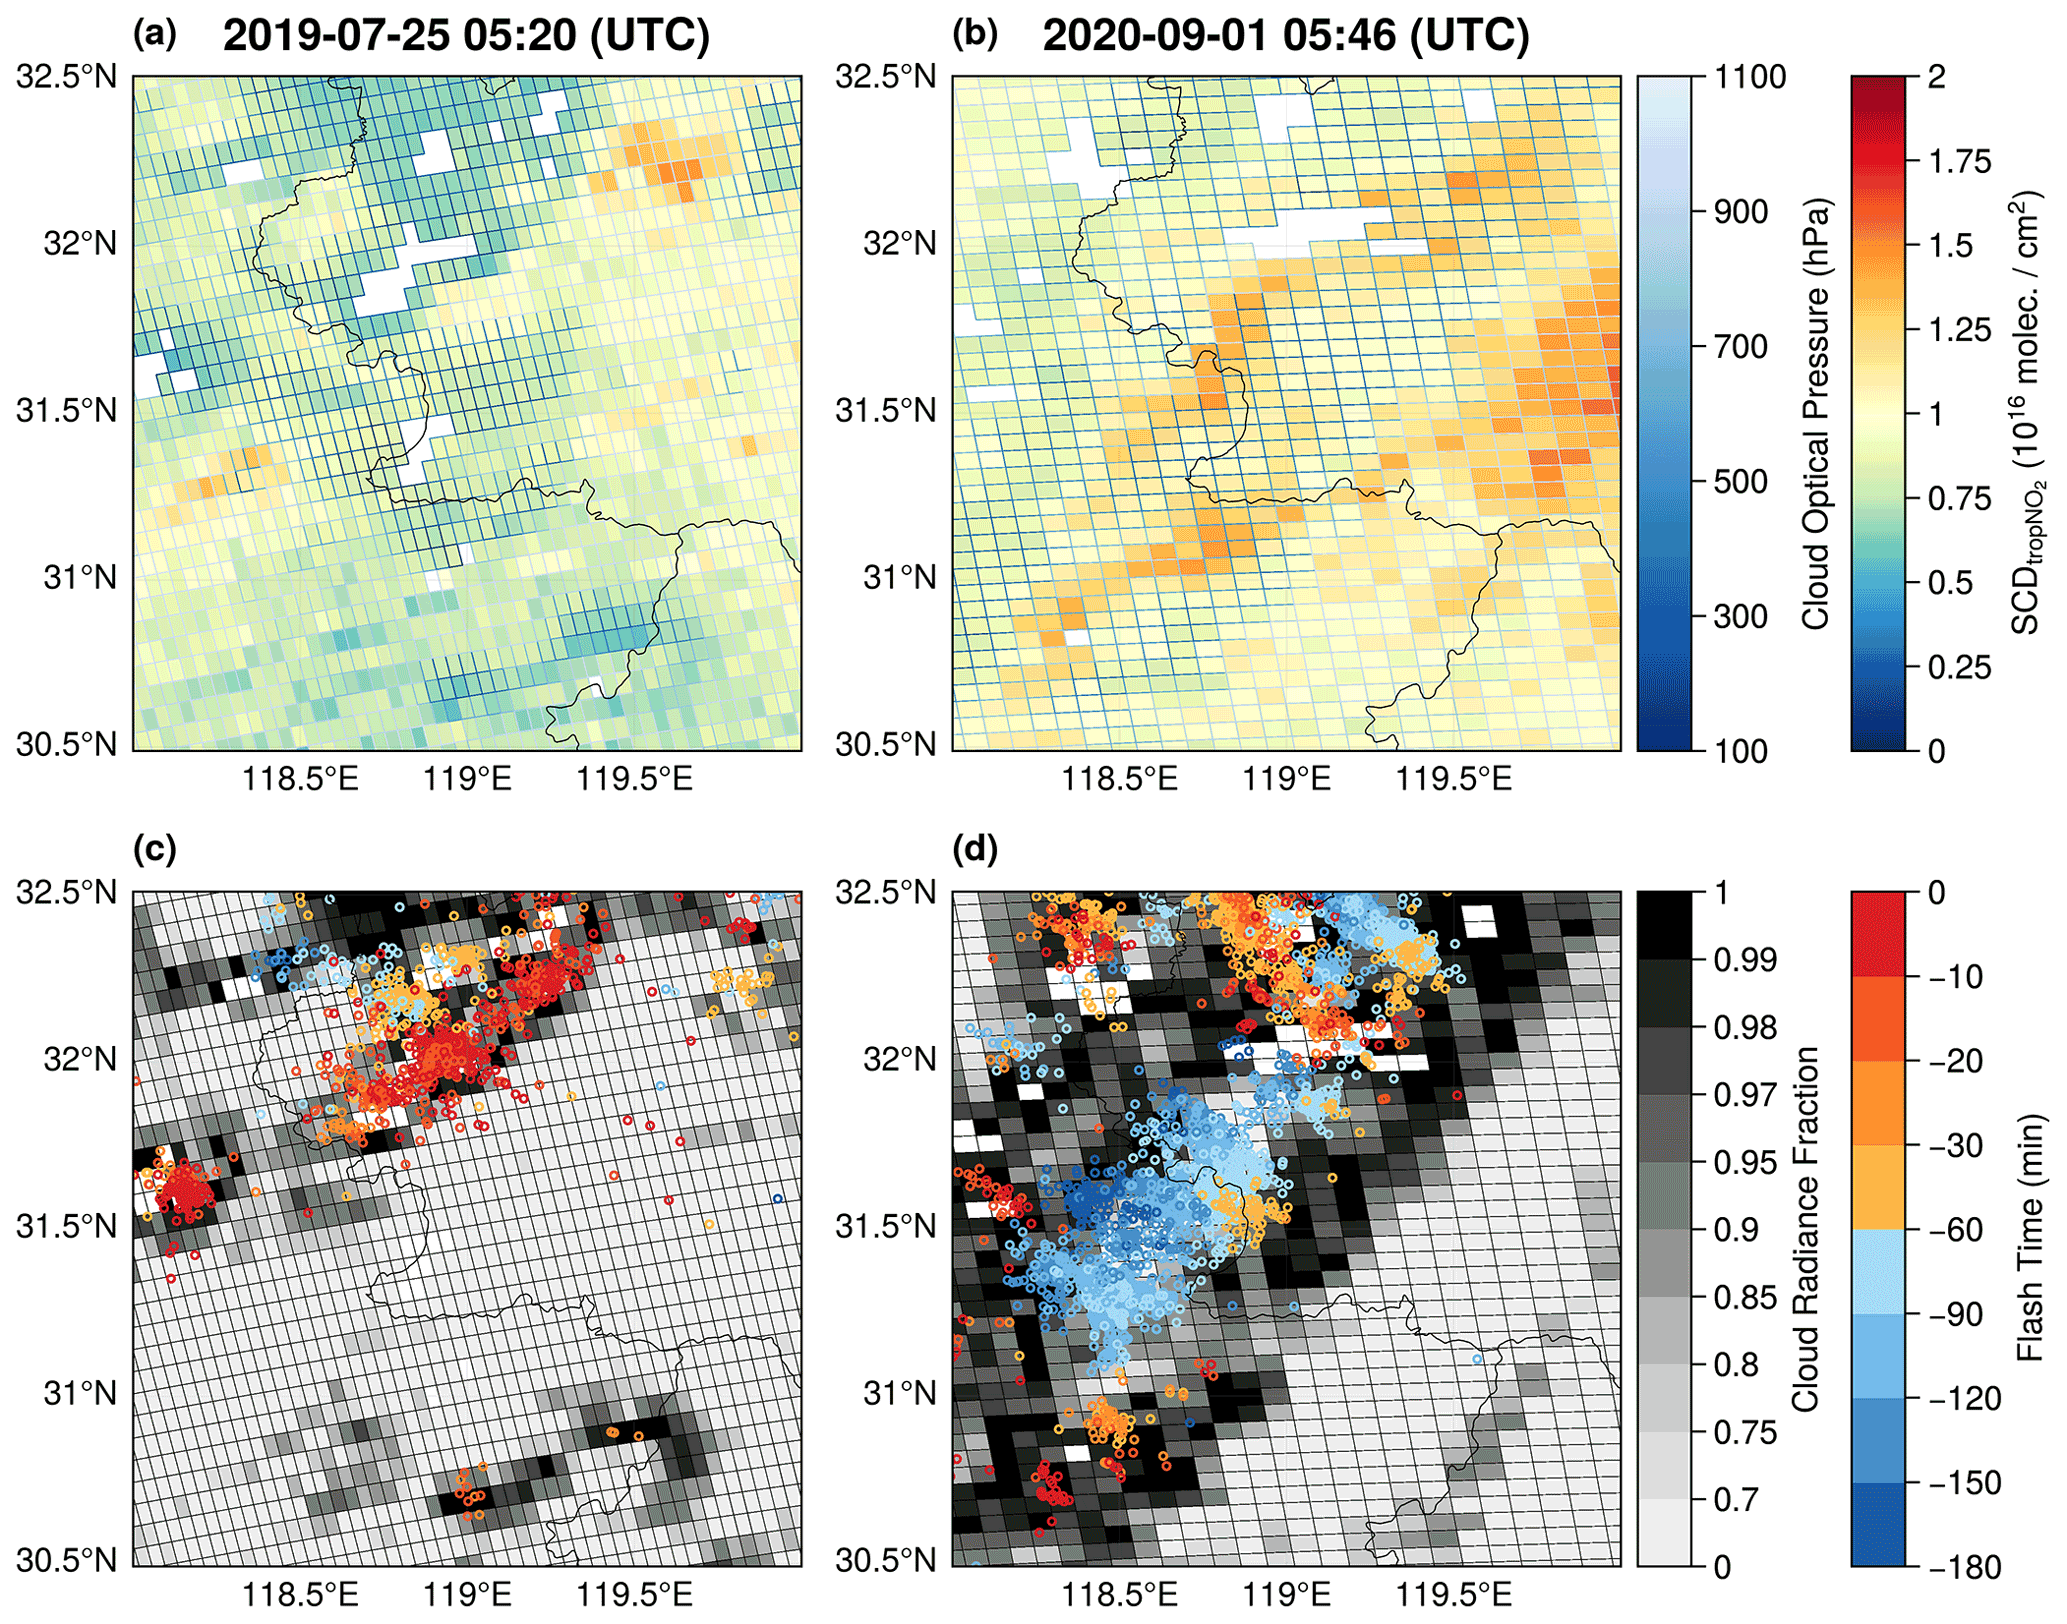
\includegraphics[width=11cm]{./figures/china_flash_scd.png}
    \caption{
    2019 年 7 月 25 日(左)和 2020 年 9 月 7 日(右)的个例。
    (a,b)对流层 NO$_2$ 斜柱浓度($S_{\ch{NO2}}$,填充色)和云压(线条颜色)。
    这些白色网格单元代表缺失的 TROPOMI 数据,黑色实线为江苏省。
    (c,d)NO$_2$ 窗区中的云辐射分数和闪电。闪电的颜色取决于相对于TROPOMI过境的发生时间。\\
    Figure \ref{fig:china_flash_scd}. Events on 25 July 2019 (left) and 07 September 2020 (right).
    (a, b) The tropospheric NO$_2$ slant column density ($S_{\ch{NO2}}$, filled color) and cloud optical pressure (line color).
    These white grid cells stand for missing TROPOMI data.
    The solid black border is Jiangsu province.
    (c, d) The cloud radiance fraction in the NO$_2$ window and flashes whose color depends on the occurring time relative to the TROPOMI overpass time.
    }
    \label{fig:china_flash_scd}
\end{figure}


\begin{figure}[H]
    \centering
    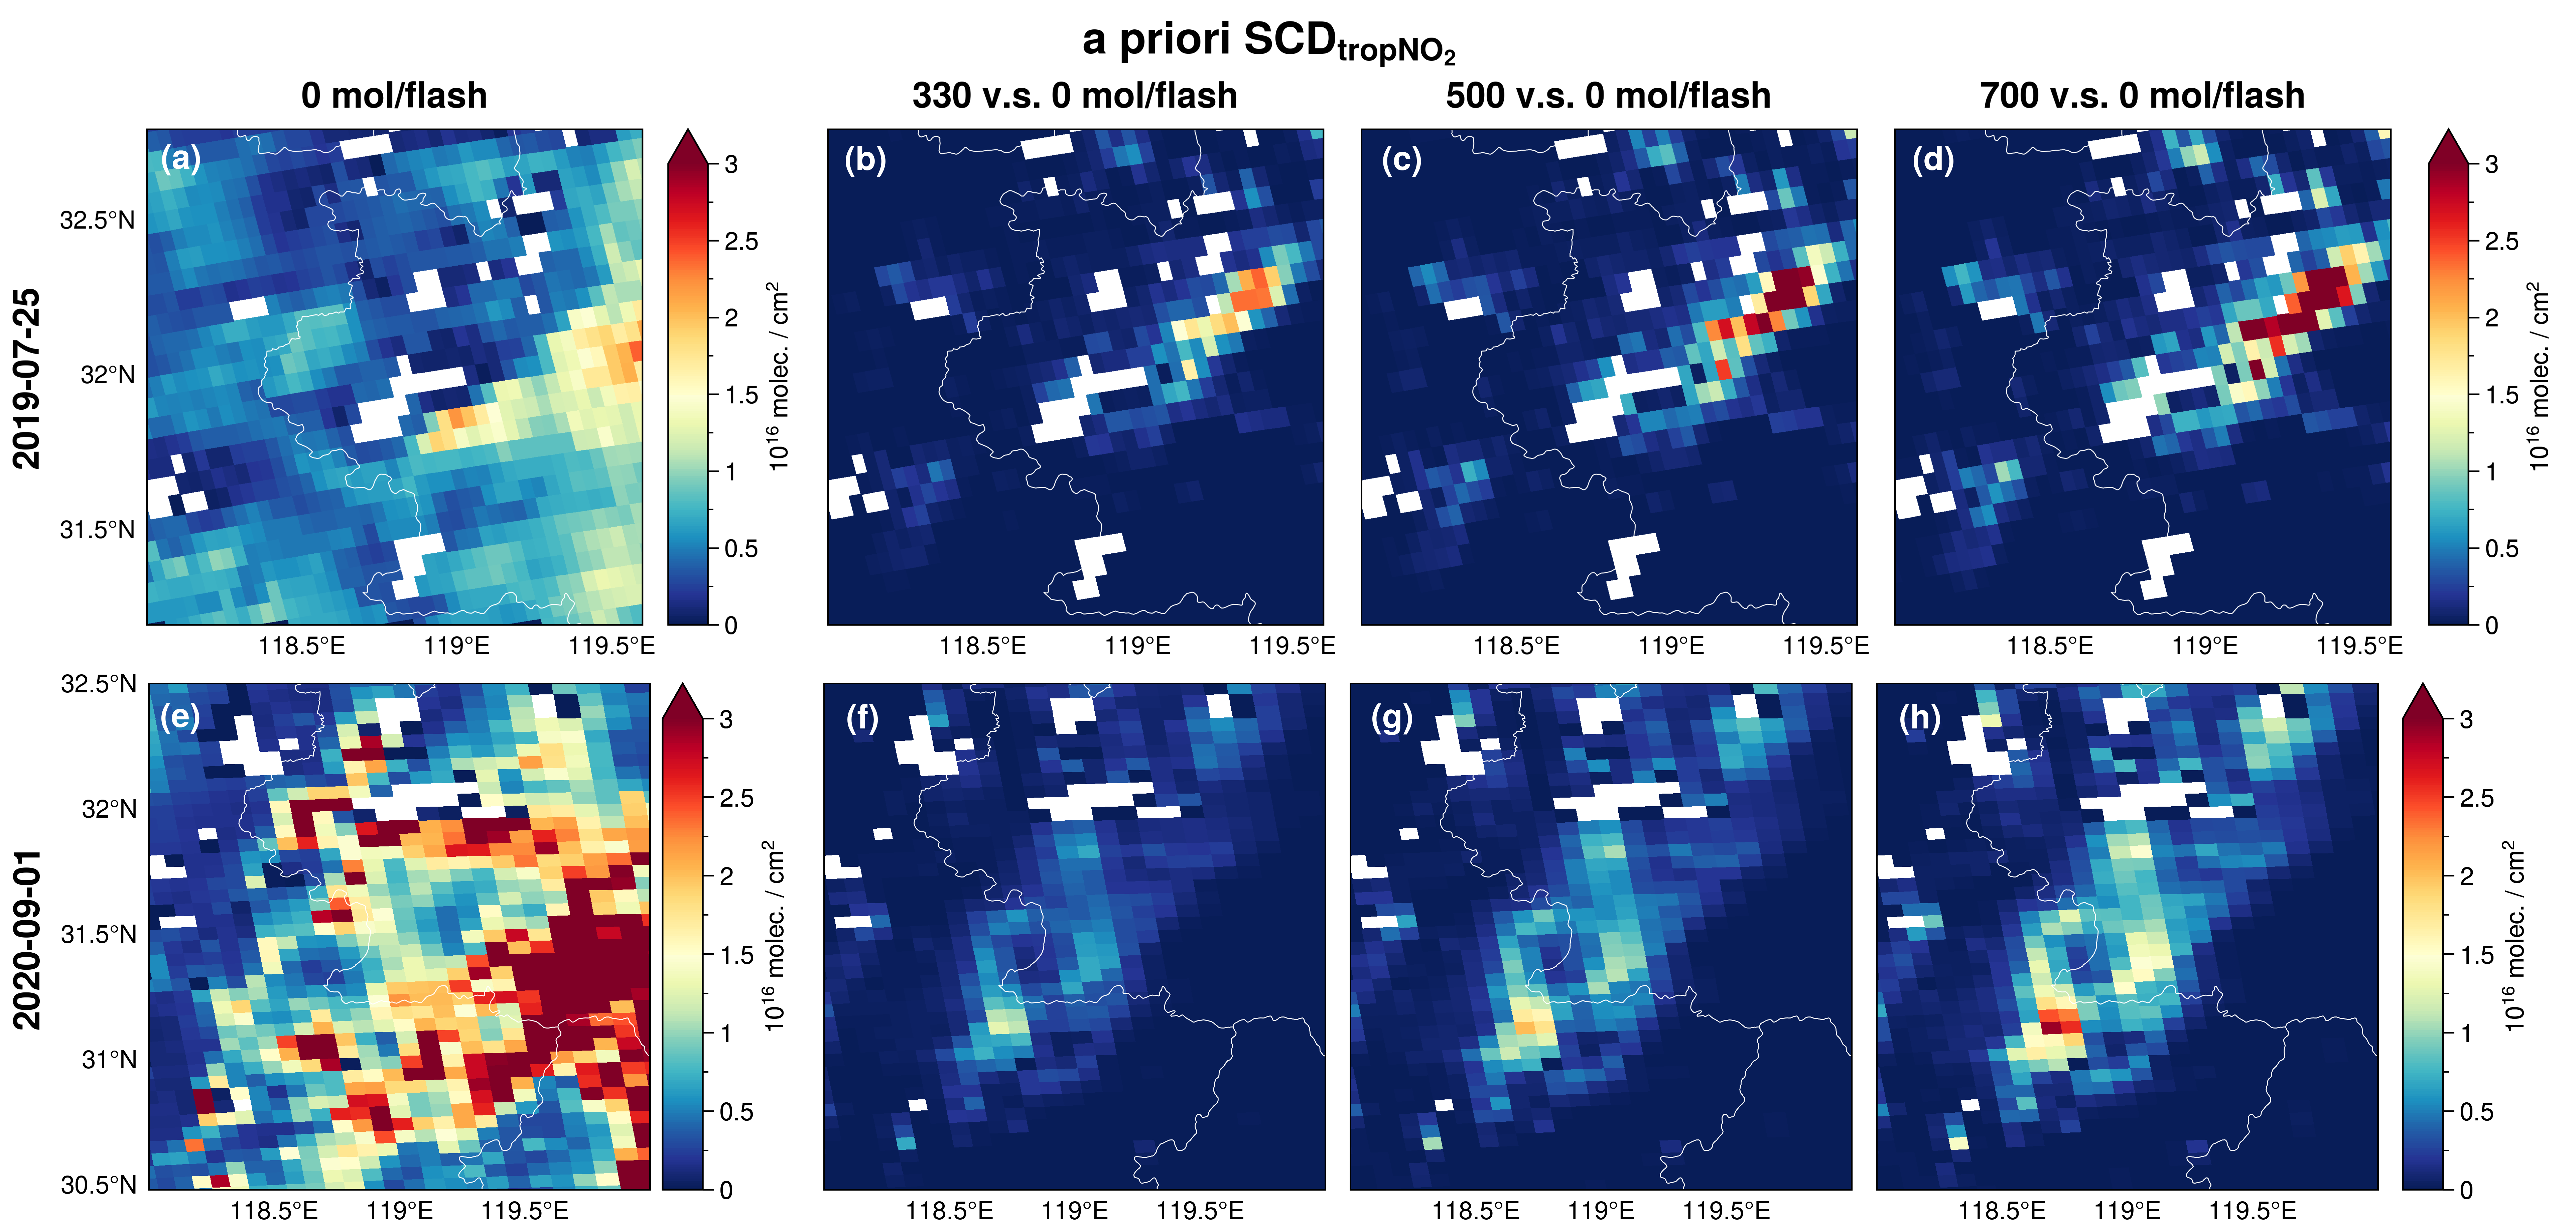
\includegraphics[width=14cm]{./figures/s5p_apriori_scd.png}
    \caption{使用不同闪电NO排放条件下WRF-Chem的NO$_2$结果重新计算得到的对流层NO$_2$斜柱浓度($S_{\ch{NO2}}$)。
    (a,e)0 mol每闪电;(b,f)330 mol每闪电;(c,g)500 mol每闪电;(d,h)700 mol每闪电。\\
    Figure \ref{fig:s5p_apriori_scd}. The tropospheric NO$_2$ slant column density ($S_{\ch{NO2}}$) recalculated using the WRF-Chem results with different lightning NO settings: (a, e) 0 mol/flash, (b, f) 330 mol/flash, (c, g) 500 mol/flash and (d, h) 700 mol/flash.
    }
    \label{fig:s5p_apriori_scd}
\end{figure}


具体而言,对流旺盛处(f$_r$ $\geq$ 0.7)的$S_{\ch{NO2}}$小于其他区域。
这与之前针对具有高闪电密度的大规模对流系统研究结果相反\citep{Beirle.2009}。
导致这一差距的因素有四点:云顶高度、闪电次数、闪电发生时间和背景NO$_2$浓度。
由于TROPOMI只能探测到处于云层上方的LNO$_2$,因此当f$_r$ $\sim$ 1时,
闪电次数不足或对流较弱都可能导致对流旺盛区的$S_{\ch{NO2}}$更小,
即如果f$_r$<1,破碎或稀薄云层下方的污染NO$_2$会部分被TROPOMI探测到,
WRF-Chem的先验$S_{\ch{NO2}}$敏感性试验可以清楚地解释这种现象(图\ref{fig:s5p_apriori_scd})。
具有低f$_r$和高$S_{\ch{NO2}}$像素源自于背景 NO$_2$ 污染(图\ref{fig:s5p_apriori_scd} a,e),
但与没有LNO$_2$贡献的低$S_{\ch{NO2}}$相比,对流层上层LNO$_2$增加的$S_{\ch{NO2}}$仍然可见(图\ref{fig:s5p_apriori_scd}b--d,f--h)。

在\ref{sec:us}节和\ref{sec:china}节中,我们利用对流旺盛时的卫星观测来估算 LNO$_x$产率。
然而,由于 TROPOMI 的像素饱和和对流区域的有限覆盖(图\ref{fig:china_flash_scd}c),
该方法难以应用于范围较小发展强的对流(2019年个例)。
因此,我们尝试不对云量加以限制,将该方法应用于消散期的对流(2020年个例,图\ref{fig:china_flash_scd}d)。
如图 \ref{fig:china_vcd_lnox}b--c 所示,闪电与TROPOMI的过境时间差大于 30 分钟但小于 3 小时。
由于 NO$_2$ 的寿命在对流附近为 $\sim$ 3(2--12)小时 \citep{Nault.2016},
2020年个例的TROPOMI观测数据仍可以用于估算LNO$_x$。
平均 LNO$_x$产率(mol/flash)的定义如下:


\begin{equation} \label{eq:lnox}
PE_{LNO_x} = \sum_{p} V_i A_i / \sum_{N} F_j e^{-(t_0 - t_j) / \tau}
\end{equation}

其中 $p$ 代表受 LNO$_x$ 影响的像素,
$V_i$(mol/m$^2$)是像素 $i$ 上LNO$_x$ 垂直柱浓度 ($V_{\ch{LNO_x}}$ = $S_{\ch{NO2}}$ / $AMF_{\ch{LNO_x}}$),
面积称为 A$_i$ (m$^2$),
$N$ 是 对 $V_{\ch{LNO_x}}$ 做出贡献的闪电总数,
指数部分考虑了每个闪电(F$_j$)排放的NO$_x$ 的寿命。
具体而言,AMF$_{\ch{LNO_x}}$源于式(\ref{eq:AMF_LNO2}),
t$_0$是TROPOMI的过境时间,
t$_j$是闪电的发生时间,
$\tau$为近对流的NO$_x$寿命(3 小时)。

由于消散的对流已产生了足够多的闪电,并且对流处对流层上层的风从西北偏西吹向东南偏东(图\ref{fig:china_vcd_lnox}a),
$V_{\ch{LNO_x}}$的范围仍然可以清楚地识别(图\ref{fig:china_vcd_lnox} 中的虚线矩形)。
幸运的是,有一条$V_{\ch{LNO_x}}$低值带将南北对流分开。
经过仔细选择,计算得到的LNO$_x$产率为60 mol NO$_x$每闪电。
虽然有些与 $V_{\ch{LNO_x}}$ 相关的闪电在选择的区域之外,
它对LNO$_x$产率的影响仅 $\sim$ 2 mol,在下节的不确定性评估范围内。


\begin{figure}[H]
    \centering
    
\includegraphics[width=16cm]{./figures/china_vcd_lnox.png}
    \caption{
    背景为LNO$_x$垂直柱浓度($V_{\ch{LNO_x}}$)的分布。
     白色矩形是为手动选择的用于 LNO$_x$产率估算的区域。
     (a)中叠加的箭头是 WRF-Chem 模拟的 500 hPa 水平风;
     (b)和(c)中的点是闪电,其颜色取决于相对于 TROPOMI 过境的发生时间。\\
    Figure \ref{fig:china_vcd_lnox}. The background is the distribution of LNO$_x$ vertical column densities ($V_{\ch{LNO_x}}$).
    The white rectangles are manually selected regions for the LNO$_x$ production efficiency estimation.
    The overlayed wind arrows in (a) are the 500 hPa horizontal wind simulated by WRF-Chem.
    The dots in (b) and (c) are the flashes whose color depends on the occurring time relative to the TROPOMI overpass time.
    }
    \label{fig:china_vcd_lnox}
\end{figure}



\subsection{估算的影响因素及不确定性分析} \label{sec:uncertainty_china}

根据 \citet{Allen.2019} 和 \citet{Zhang.2020b},LNO$_x$ 的不确定性由 LNO$_x$ 寿命、闪电探测效率、
NO/NO$_2$ 比例、LNO 廓线和其他来源决定(表\ref{table:uncertainty_china})。
我们将NO$_2$的寿命替换为2和6 h,得到的不确定性为27\%,而将IC与CG的比值改为2 :1 和 4:1,得到的不确定性也为27\%。
根据 \citet{Allen.2019} 我们将由模拟引起的 NO/NO$_2$ 比例的不确定性设置为 30\%。
此外我们利用330 和 700 mol NO每闪电的WRF-Chem敏感性试验结果,得到与LNO廓线有关的不确定性为 26\%。
此外,与平流层垂直柱浓度[$\pm$ 10$^{14}$ molec. cm$^2$, \citet{VanGeffen.2022}]相关的不确定性为 7\%。
而由其他可能误差源引起的不确定性难以量化,比如斜柱浓度中的系统误差、云压和由对流重新分布的 NO$_2$,
根据 \citet{Allen.2021a}我们设其为10\%。
假设误差之间没有相关性,总不确定性(56\%)即为所有单个不确定性平方和的平方根。
因此,LNO$_x$产率为60 $\pm$ 33 mol NO$_x$每闪电,
该数值低于我们(90 $\pm$ 50 mol NO$_x$每闪电)以及\citet{Allen.2021a}(120 $\pm$ 65 mol NO$_x$每闪电)在美国大陆的研究结果,
因此,在未来的研究中还需对中国地区进行范围更广的探讨,从而估算区域性的LNO$_x$产率。


\begin{table*}[H]
\footnotesize
\centering
\caption{LNO$_{\ch{x}}$产率估算的不确定性\\
Table \ref{table:uncertainty_china}. Uncertainties for the estimation of LNO$_\textrm{x}$ production efficiency.}
\begin{tabularx}{.8\textwidth}{c X}
\hline
来源 & \makecell[cc]{不确定性 (\%)} \\
\hline
LNO$_x$ 寿命                & \makecell[cc]{27\%} \\
闪电探测效率                  & \makecell[cc]{27\%} \\
NO/NO$_2$ 比例               & \makecell[cc]{30\%} \\
LNO 廓线                     & \makecell[cc]{26\%} \\
平流层垂直柱浓度                & \makecell[cc]{7\%} \\
其他                          & \makecell[cc]{10\%} \\
\hline
净不确定性                             & \makecell[cc]{56\%} \\
\hline
\end{tabularx}
\label{table:uncertainty_china}
\end{table*}


\section{本章小结}

本章建立了基于卫星遥感NO$_2$柱浓度定量分析不同污染背景下LNO$_2$的
计算方法,得到了不同污染程度地区的LNO$_x$产率,并与其他NO$_x$排放源进行了对比。主要结论如下:

\begin{enumerate}[label=(\arabic*), labelindent=\parindent, leftmargin=0pt, widest=0, itemindent=*, topsep=0pt, partopsep=0pt, parsep=0pt]

\item 针对清洁地区(北极)的深对流,我们利用极轨卫星在北极地区连续过境的特性,
开发了TROPOMI LNO$_2$柱浓度高值区的自主识别系统,提出了通过相邻过境数据来定量 LNO$_2$ 寿命和产率的方法。

\item 2019--2021年6--8月的分析结果表明,北极地区对流附近的LNO$_2$寿命为3 h,
与污染地区的LNO$_2$寿命相似,例如美国地区的3 h \citep{Nault.2017}。
北极陆地地区的LNO$_2$ 产率 [2.0(1.3--3.1)mol每闪击] 与美国的结果(1.6 $\pm$ 0.1 mol每闪击)也相近\citep{Lapierre.2020}。
此外,北极海洋性闪电产生的 NO$_2$是陆地性闪电的6倍。
因此,当闪电在北极海洋和陆地上增加相同数量时,海洋性闪电将产生更多的 LNO$_2$。
基于得到的LNO$_2$产率,我们进一步得出北极地区夏季(6--8 月)LNO$_x$ 的平均排放量为219吨氮,
约等于该地区人为 NO$_x$ 排放量的 5\%。

\item 针对污染地区的深对流,我们利用WRF-Chem的高分辨率模拟结果定义了LNO$_2$和LNO$_x$的大气质量因子(AMF),
从而得到包含了云下LNO$_2$和LNO$_x$的柱浓度。
% 我们利用云辐射分数、地基探测的闪电阈值、模拟的闪电数$\geq$1000 和云上LNO$_2$占比$\geq$50\%来确保WRF-Chem 成功模拟出对流并且LNO$_2$能够被OMI检测。
由于新定义的AMF考虑了对流层的背景污染,因此该方法同时适用于清洁和污染区域。

\item 2014年5--8月的分析结果表明,美国大陆的夏季 LNO$_2$ 和 LNO$_x$平均产率为
32 $\pm$ 15 mol NO$_2$每闪电、90 $\pm$ 50 mol NO$_x$每闪电、6 $\pm$ 3 mol NO$_2$每闪击,以及17 $\pm$ 10 mol NO$_x$每闪击。
由于现阶段其他地区(如中国和印度)NO$_2$ 污染比美国大陆严重,因此LNO$_x$的估算有必要详细考虑NO$_2$背景污染。
此外,区域和全球模式还需开发更为完善的闪电参数化来提高局地和全球范围内LNO$_x$排放估算的准确性。

\item 2019年和2020年中国东南部的两个对流个例分析表明,TROPOMI 的像素饱和效应导致无法获得旺盛对流处的LNO$_x$,
因此我们提出计算消散阶段的LNO$_x$,并得出中国东南部的LNO$_x$产率为 60 $\pm$ 33 mol NO$_x$每闪电。
未来的研究可同时利用旺盛和消散对流期间 OMI或TROPOMI 的有效数据,从而量化和改进 LNO$_x$ 的产量估计。

\end{enumerate}

	%!TEX root = ../thesis.tex

\chapter{深对流对氮氧化物垂直分布的影响}

\section{模式设置}

\subsection{气象及化学设置}

\subsection{闪电参数化}

% \section{模式评估}


\section{结果与讨论}

\subsection{云上二氧化氮柱密度的分布}

由上一章分析可知,将卫星观测所得的NO$_2$柱密度和闪电数据相结合,可以得出LNO$_2$的产率,然而NO$_2$的垂直分布无法由此直接得出。
因此本章将采用云切片的方法,利用卫星针对不同高度深厚对流云的观测,得到云间的平均NO$_2$浓度,从而获得对流状态下的NO$_2$平均廓线,并与全球模式进行对比分析。

图\ref{fig:no2geo_tropomi}为TROPOMI观测的2019年中低纬度云上NO$_2$分布图,
云的中心气压分别为330 hPa、450 hPa、570 hPa、670 hPa、770 hPa、以及 870 hPa。
其中330 hPa和450 hPa的云上NO$_2$高值区位于美国东南部、中国沿海地区、中国华北地区、墨西哥、巴拿马、
古巴、孟加拉国、尼泊尔、新德里、非洲中部、和热带辐合带,
这些地区与图\ref{fig:no2_ltngcount}(c)的闪电高值区相对应。
前人研究表明,中低纬LNO$_2$的峰值分布在100--500 hPa之间\citep{Pickering.1988,Ott.2010,Luo.2017},
故330 hPa和450 hPa的云上NO$_2$包含了LNO$_2$的贡献。
然而TROPOMI的晴空NO$_2$平均柱密度产品显示(图\ref{fig:no2_ltngcount}b),这些地区属于NO$_2$高污染区,所以上对流层的NO$_2$也有来自深对流垂直输送的污染NO$_2$。
中云(570 hPa和670 hPa)的云上NO$_2$有效数据更多,云上NO$_2$高值区包含了高云(330 hPa和450 hPa)的云上NO$_2$高值区。
其中污染NO$_2$的贡献更为明显,与晴空NO$_2$平均柱密度产品分布更为接近,如中国东部、欧洲、和美国东北部的工业源以及非洲中部的生物质燃烧。
污染物排放在低云(770 hPa和870 hPa)的云上NO$_2$最为明显,然而由于热带地区云顶较高,有效数据更少。


\begin{figure}[htbp]
    \centering
    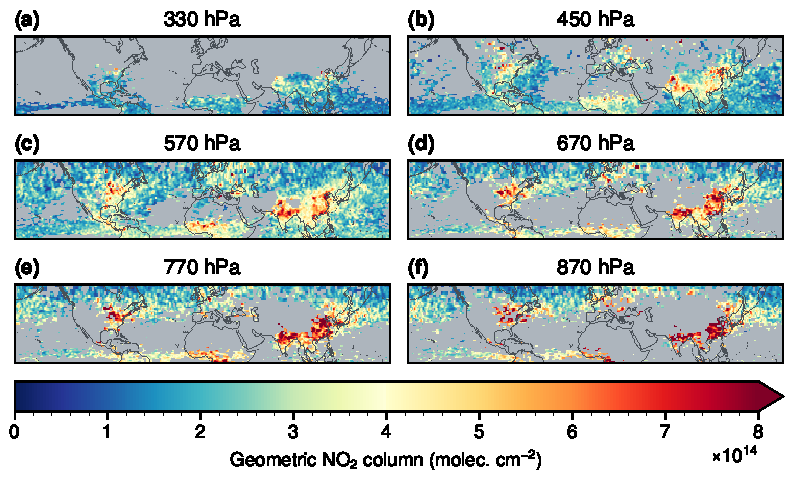
\includegraphics[width=15cm]{./figures/no2geo_tropomi.pdf}
    \caption{
    2019年6--8月北半球中低纬度TROPOMI观测的云上NO$_2$柱密度分布图:
    高云([a] 330 hPa 和 [b] 450 hPa),中云 ([c] 570 hPa 和 [d] 670 hPa),
    及低云 ([e] 770 hPa 和 [f] 870 hPa)。 \\
    NO$_2$ above cloud at the middle and low latitudes for June--August in 2019:
    High clouds ([a] 330 hPa, [b] 450 hPa), middle clouds ([c] 570 hPa, [d] 670 hPa),
    and low clouds ([e] 770 hPa, [f] 870 hPa).
    }
    \label{fig:no2geo_tropomi}
\end{figure}


\begin{figure}[htbp]
    \centering
    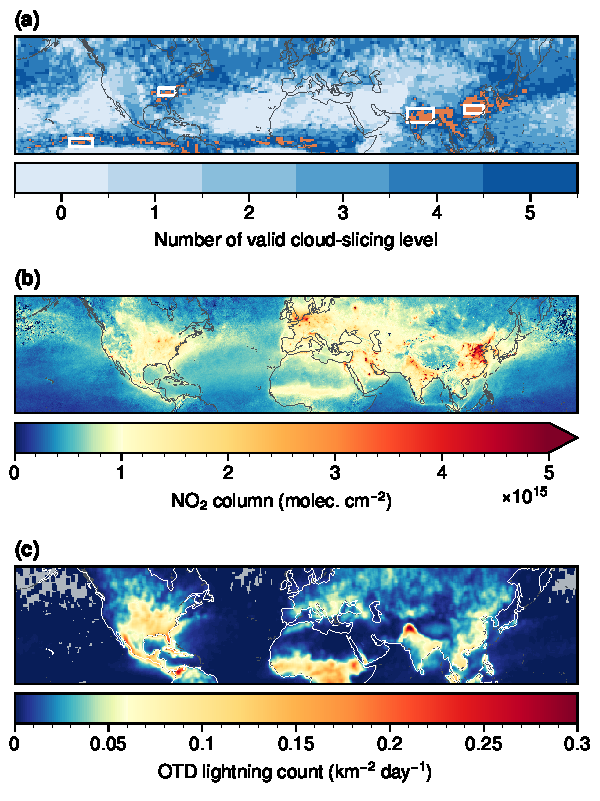
\includegraphics[width=13cm]{./figures/no2_ltngcount.pdf}
    \caption{
    (a) 云切片的总有效气压层数,层数$\leq$ 5为蓝色,= 6 为橙色。
    (b)2019--2021年中低纬度夏季(6--8月)TROPOMI测得的NO$_2$平均柱密度。
    (c) 1995--2014年中低纬度夏季(6--8月)LIS/OTD的闪电密度产品。 \\
    (a) Number of total valid cloud-slicing pressure levels.
    Grids with number of levels $leq$ 5 and = 6 are filled in blue and orange, respectively.
    (b) The average TROPOMI NO$_2$ column densities at the middle and low latitudes for June--August in 2019--2021.
    (c) The average LIS/OTD lightning flash rates at the middle and low latitudes for June--August in 1995--2014.
    }
    \label{fig:no2_ltngcount}
\end{figure}

\subsection{二氧化氮的垂直分布}


上节得到的云上NO$_2$为对流层NO$_2$柱密度,柱底为云的中心气压,
通过\ref{sec:云切片算法}章的云切片算法可进一步得到每层的NO$_2$浓度,即NO$_2$廓线。

图\ref{fig:utno2_tropomi}为2019年6--8月不同高度的NO$_2$平均浓度。
与图\ref{fig:no2geo_tropomi}不同,高云处的NO$_2$浓度(图\ref{fig:utno2_tropomi}(a--b))高于中云(图\ref{fig:utno2_tropomi}(c--d))。
其中陆地上180 hPa--330 hPa间的NO$_2$为330 hPa--450 hPa间的$\approx$1.2倍,为450--570 hPa间的$\approx$2倍,
而570 hPa以下(图\ref{fig:utno2_tropomi}(d--f))陆地上的NO$_2$浓度逐渐上升。
该现象与前人的模拟和飞机观测结果相符,LNO$_2$在上对流层占主导,而污染NO$_2$在下对流层占主导\citep{Pickering.1996,Ott.2010,Laughner.2017}。


\begin{figure}[htbp]
    \centering
    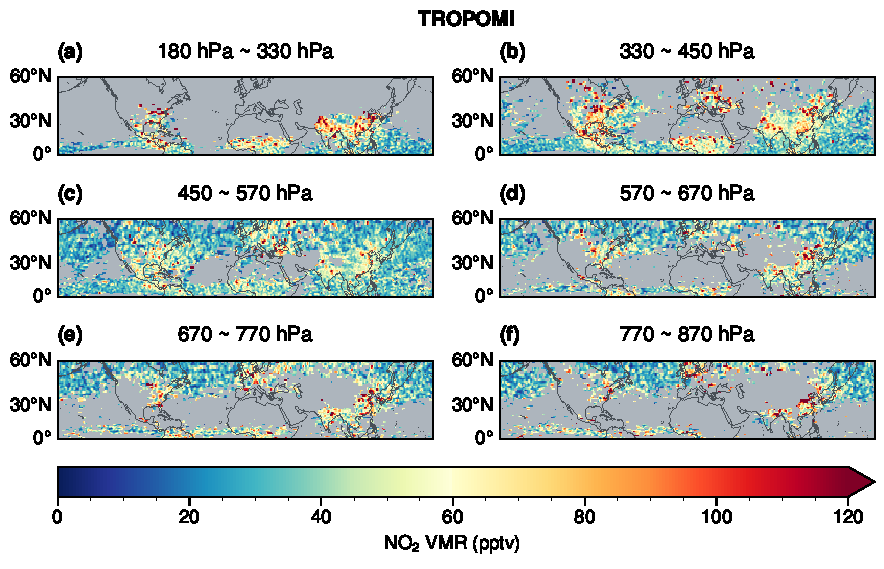
\includegraphics[width=15cm]{./figures/utno2_tropomi.pdf}
    \caption{
    TROPOMI云切片算法所得的2019年6--8月北半球中低纬度NO$_2$浓度分布图。 \\
    The NO$_2$ vertical mixing ratios derived from the cloud-slicing results of TROPOMI NO$_2$ observations at the middle and low latitudes for June--August in 2019.
    }
    \label{fig:utno2_tropomi}
\end{figure}


为了进一步分析LNO$_2$在其中的作用,我们首先将各个高度层的TROPOMI观测结果与MERRA2-GMI的模式结果相比较,
接着选取TROPOMI云切片各层均有有效数据的区域,结合过境期间模拟的LNO$_2$排放速率垂直分布进行廓线分析。
图\ref{fig:utno2_merra2}为2019年6--8月与TROPOMI对应的MERRA2-GMI NO$_2$模拟结果。
由两者浓度之差(图\ref{fig:utno2_delta})可知,无论位于陆地还是海洋,MERRA2-GMI较TROPOMI存在20--80 pptv的低估,
其中海洋上的误差可能由TROPOMI NO$_2$反演过程中低估的平流层NO$_2$柱密度或高估的辐射强度所导致\citep{VanGeffen.2020}。


\begin{figure}[htbp]
    \centering
    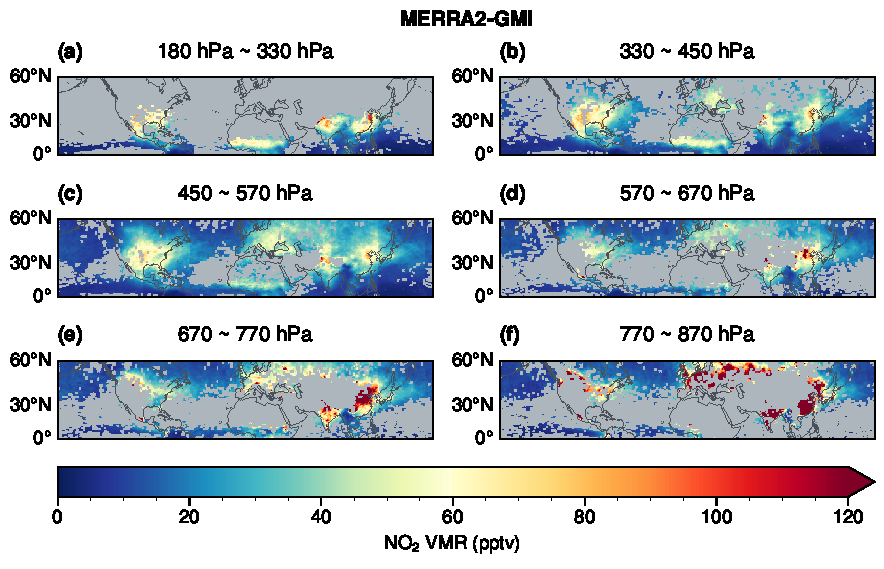
\includegraphics[width=15cm]{./figures/utno2_merra2-gmi.pdf}
    \caption{
    同图\ref{fig:utno2_tropomi}但数据为MERRA2-GMI。 \\
    Same as Fig. \ref{fig:utno2_tropomi} but for MERRA2-GMI.
    }
    \label{fig:utno2_merra2}
\end{figure}

\begin{figure}[htbp]
    \centering
    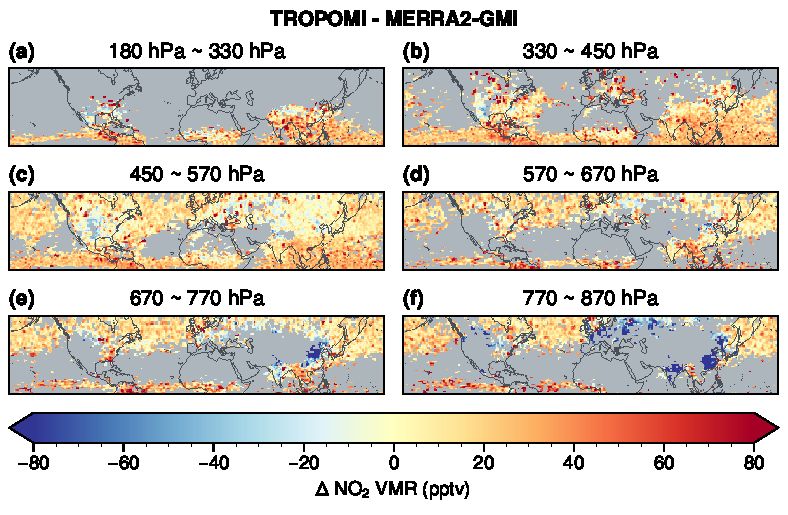
\includegraphics[width=15cm]{./figures/utno2_delta.pdf}
    \caption{
    图\ref{fig:utno2_tropomi}与图\ref{fig:utno2_merra2}之差。 \\
    Differences between Fig. \ref{fig:utno2_tropomi} and Fig. \ref{fig:utno2_merra2}.
    }
    \label{fig:utno2_delta}
\end{figure}


具体而言,高云间的NO$_2$正误差结果($\Delta$ NO$_2$ $>$ 0,图\ref{fig:utno2_delta}a和b)主要来自于北美、东欧、以及亚洲东部沿海,
这意味着MERRA2-GMI全球模式中参数化对流垂直传输污染物的强度较低,导致高云间的NO$_2$低于TROPOMI的观测值。
而高云间的NO$_2$负误差结果位于美国中部,非洲中部,以及青藏高原西南部。
美国中部和非洲中部的误差是由于MERRA2-GMI中的闪电参数化(上对流层的向上云质量通量)在该区域高估了闪电总量,从而导致NO$_2$浓度偏大\citep{Allen.2002,Allen.2010}。
由LIS/OTD数据(图\ref{fig:no2_ltngcount}c)可知,青藏高原西南部闪电强度较弱,故模式的高估主要应来自于亚洲夏季风的污染物输送。

中云的云切片结果有效范围最广,总体上来看TROPOMI和MERRA2-GMI之间误差较低(-10--30 pptv),
且两者具有相似的高值区分布:北美、东欧、印度、以及中国华北地区,这些地区与污染NO$_2$柱密度高值区对应。
中云的NO$_2$可能来源有对流输送的地表污染和污染的出流区,如中国华北地区的NO$_2$高值传输至东部的黄海(其中一部分也来自于船舶排放)。
其中$>$ 40 pptv的正误差集中于南美洲北部、缅甸、和泰国北部,由于这些地区地基NO$_2$稀缺,
所以该误差应归因于卫星反演误差还是模式NO$_x$排放源需更新,有待进一步研究。
此外,中云的负误差结果在570--670 hPa更为明显,尤其是中国的华北地区,考虑到MERRA2-GMI对流垂直输送强度较低,故而使用的排放清单中NO$_x$排放量可能过高\citep{Ziemke.2019}。

低云的云切片结果NO$_2$高值区与中云结果类似,值得注意的是云切片结果比MERRA2-GMI的数据低50--200 pptv,
该差异在中国东部和印度北部最为明显($>$ 100 pptv)。
前人研究表明,几何AMF(AMF$_{geo}$)在低云和污染条件下可达可见AMF(AMF$_{Vis}$,公式\ref{eq:AMF_NO2Vis})的两倍\citep{BelmonteRivas.2015},然而不足以解释中国东部地区的模拟值为观测值的3--5倍。
因此,该差异反映了MERRA2-GMI使用的大气化学和气候模型比对项目 (ACCMIP) 排放清单在中国东部未能及时更新。

除了各层的地理分布之外,我们选取了代表区域内云切片有效层数为6层的格点(中国南部、印度中部、美国东南部、以及太平洋,图\ref{fig:no2_ltngcount}a),进行了廓线对比分析。
由于TROPOMI在太平洋清洁地区的高估,我们将云切片结果进行校正,即除以其与MERRA2-GMI和TROPOMI比例的平均值。


\begin{figure}[htbp]
    \centering
    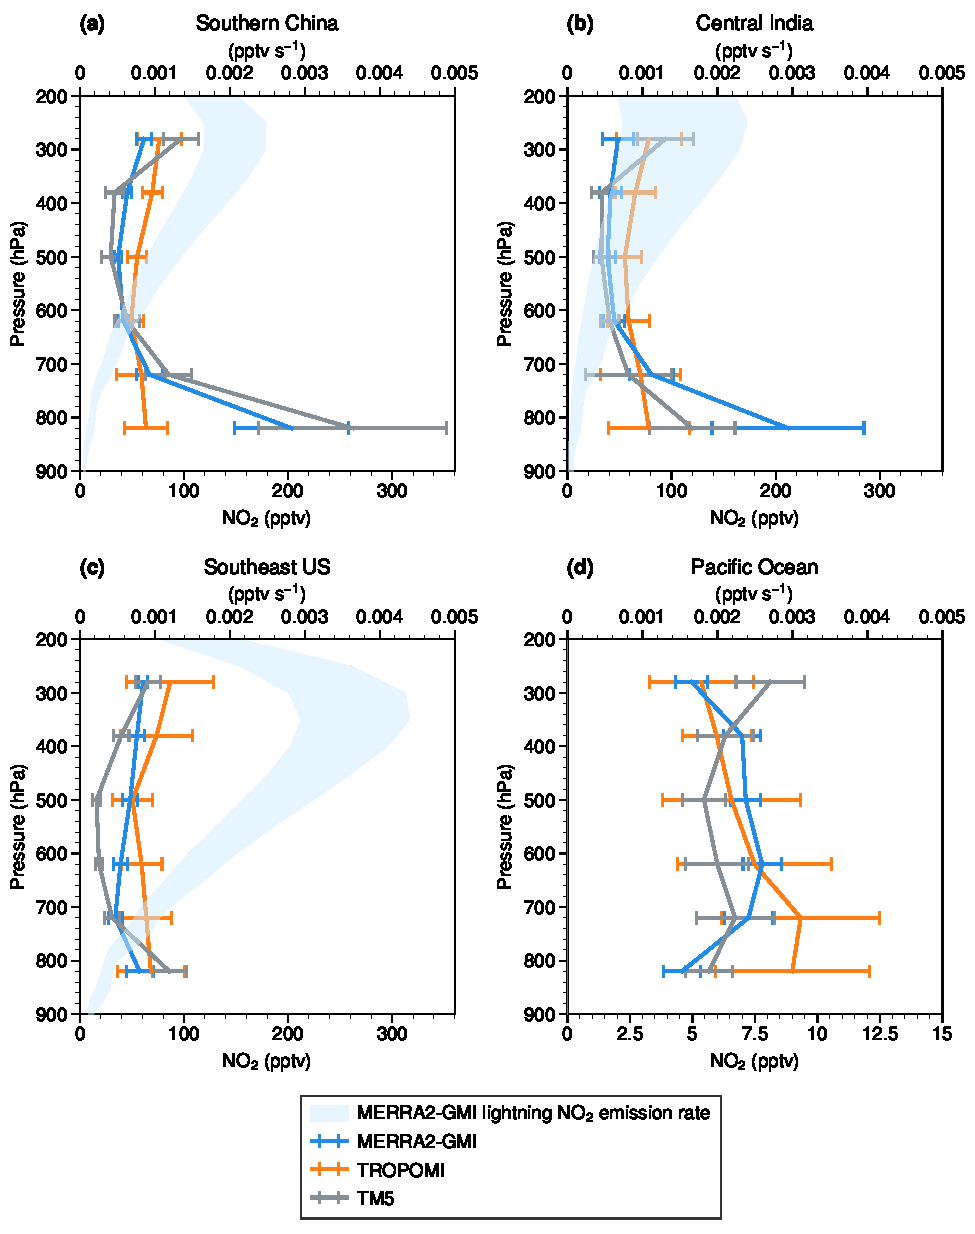
\includegraphics[width=15cm]{./figures/utno2_profile.pdf}
    \caption{
    TM5(灰色)、MERRA2-GMI(蓝色)、以及TROPOMI云切片算法(橙色)所得到的区域平均NO$_2$廓线
    (a)中国南部、(b)印度中部、(c)美国东南部、(d)太平洋 。
    浅蓝色填充部分为下午地方时2点的MERRA2-GMI闪电NO$_2$排放速率,
    其中廓线的误差棒和填充范围为平均值$\pm$标准差。\\
    Regional average NO$_2$ profiles obtained by TM5 (gray), MERRA2-GMI (blue), and TROPOMI cloud slice algorithm (orange)
    (a) southern China, (b) central India, (c) southeastern United States, and (d) Pacific Ocean.
    The light blue filled part is the MERRA2-GMI lightning NO$_2$ emission rate at local 2 p.m.,
    where the error bars and filled ranges of the profiles are the mean values $\pm$ standard deviations.
    }
    \label{fig:utno2_profile}
\end{figure}

总之,TROPOMI的观测结果和MERRA2-GMI的模拟结果在对流层各层存在显著的一致性,
尤其是陆地的污染地区,而局部的差异表明云切片方法可以用来检验模式的对流垂直输送和水平输送能力,LNO$_x$的产量和分布、以及使用的排放源清单。






% \subsection{闪电氮氧化物的影响} \label{subsect:lnox_affects_tropomi}
% \subsection{不同排放源对氮氧化物垂直分布的贡献}
\subsection{闪电氮氧化物对TROPOMI产品的影响}  \label{subsect:lnox_affects_tropomi}


在利用卫星观测计算LNO$_x$产率之前,我们首先探讨了LNO$_x$对官方NO$_2$柱浓度产品的影响。
图\ref{fig:flash_scd}(a--d)将对流层NO$_2$斜柱浓度(S$_{\textrm{NO$_2$}}$)的分布与观测的闪电分布进行了比较。
尽管由于探测器饱和和光晕效应,闪电最活跃像素上的S$_{\textrm{NO$_2$}}$无效,但附近或对流出流区仍有有效数据。
在2019年的个例中,闪电发生在TROPOMI过境前不到30分钟,但2020年的个例中既有新生的也有老化的LNO$_2$(图\ref{fig:flash_scd}(d))。

具体而言,对流旺盛处((f$_r$) $\geq$ 0.7)的S$_{\textrm{NO$_2$}}$小于其他区域。
这与之前针对具有高闪电密度的大规模对流系统的研究结果相反\citep{Beirle.2009}。
导致这一差距的因素有四点:云顶高度、闪电次数、闪电发生时间和背景NO$_2$浓度。
由于TROPOMI只能探测到处于云层上方的LNO$_2$,因此当fr $\approx$ 1时,闪电次数不足或对流较弱都可能导致对流旺盛区的S$_{\textrm{NO$_2$}}$更小。
即如果f$_r$<1,则破碎或稀薄云层下方的污染NO$_2$则会部分被TROPOMI探测到。
而WRF-Chem的先验S$_{\textrm{NO$_2$}}$敏感性试验可以清楚地解释这种现象(图\ref{fig:s5p_apriori_scd})。
具有低f$_r$和高S$_{\textrm{NO$_2$}}$像素源自于背景 NO$_2$ 污染(图\ref{fig:s5p_apriori_scd}(a)和(e)),
但与没有LNO$_2$贡献的低S$_{\textrm{NO$_2$}}$相比,上对流层LNO$_2$增加的S$_{\textrm{NO$_2$}}$仍然可见(图\ref{fig:s5p_apriori_scd}(b)--(d) 和 (f)--(h))。

为了研究LNO$_x$对AMF$_\textrm{trop}$和AMF$_\textrm{LNO$_x$}$计算的重要性,我们将LNO产率的上限700 mol NO 每闪电\citep{Ott.2010}应用于WRF-Chem 。
接着我们通过独立替换三个对流层层中的NO$_2$廓线:对流层中层(MT,800 到 400 hPa)、对流层上层(UT,400 到 150 hPa)和整个对流层(地表到对流层顶)。
除非另有说明,否则后文AMF的变化是通过增加LNO$_x$获得的。
如图\ref{fig:s5p_amf_diff}显示,AMF变化主要由检测灵敏度高的上对流层LNO$_x$所控制\citep{Beirle.2009,Laughner.2017},且LNO$_x$产量在该高度达到峰值(图\ref{fig:nox_profile})。
虽然两种情况下AMF均降低了5\%--40\%,但AMF$_\textrm{trop}$的变化($\Delta$AMF$_\textrm{LNO$_x$}$)具有区域特异性。
可根据闪电活动对其进行分类:新生闪电区(MT ΔAMF\%)、闪电下风向(MT $\Delta$AMF$_\textrm{trop}$>20\%)和闪电老化区(UT $\Delta$AMF$_\textrm{trop}$>20\%)。
图\ref{fig:amf_contribution}(a)说明了云压(p$_{cloud}$)和f$_r$在这三个区域上的关系。
云层高于400 hPa(p$_{cloud}$< 400 hPa),新生闪电区的像素上f$_r$大于0.8,但闪电老化区和闪电下风向都有低于400 hPa的云层。
这与图\ref{fig:nox_profile}中的平均云压一致,并解释了为什么UT $\Delta$AMF$_\textrm{trop}$ > 20\% 在图\ref{fig:s5p_amf_diff}(b)i 和 (b)iii 中存在,这也正表明了在闪电老化区估算LNO$_x$的可能性。


\begin{figure}[htbp]
    \centering
    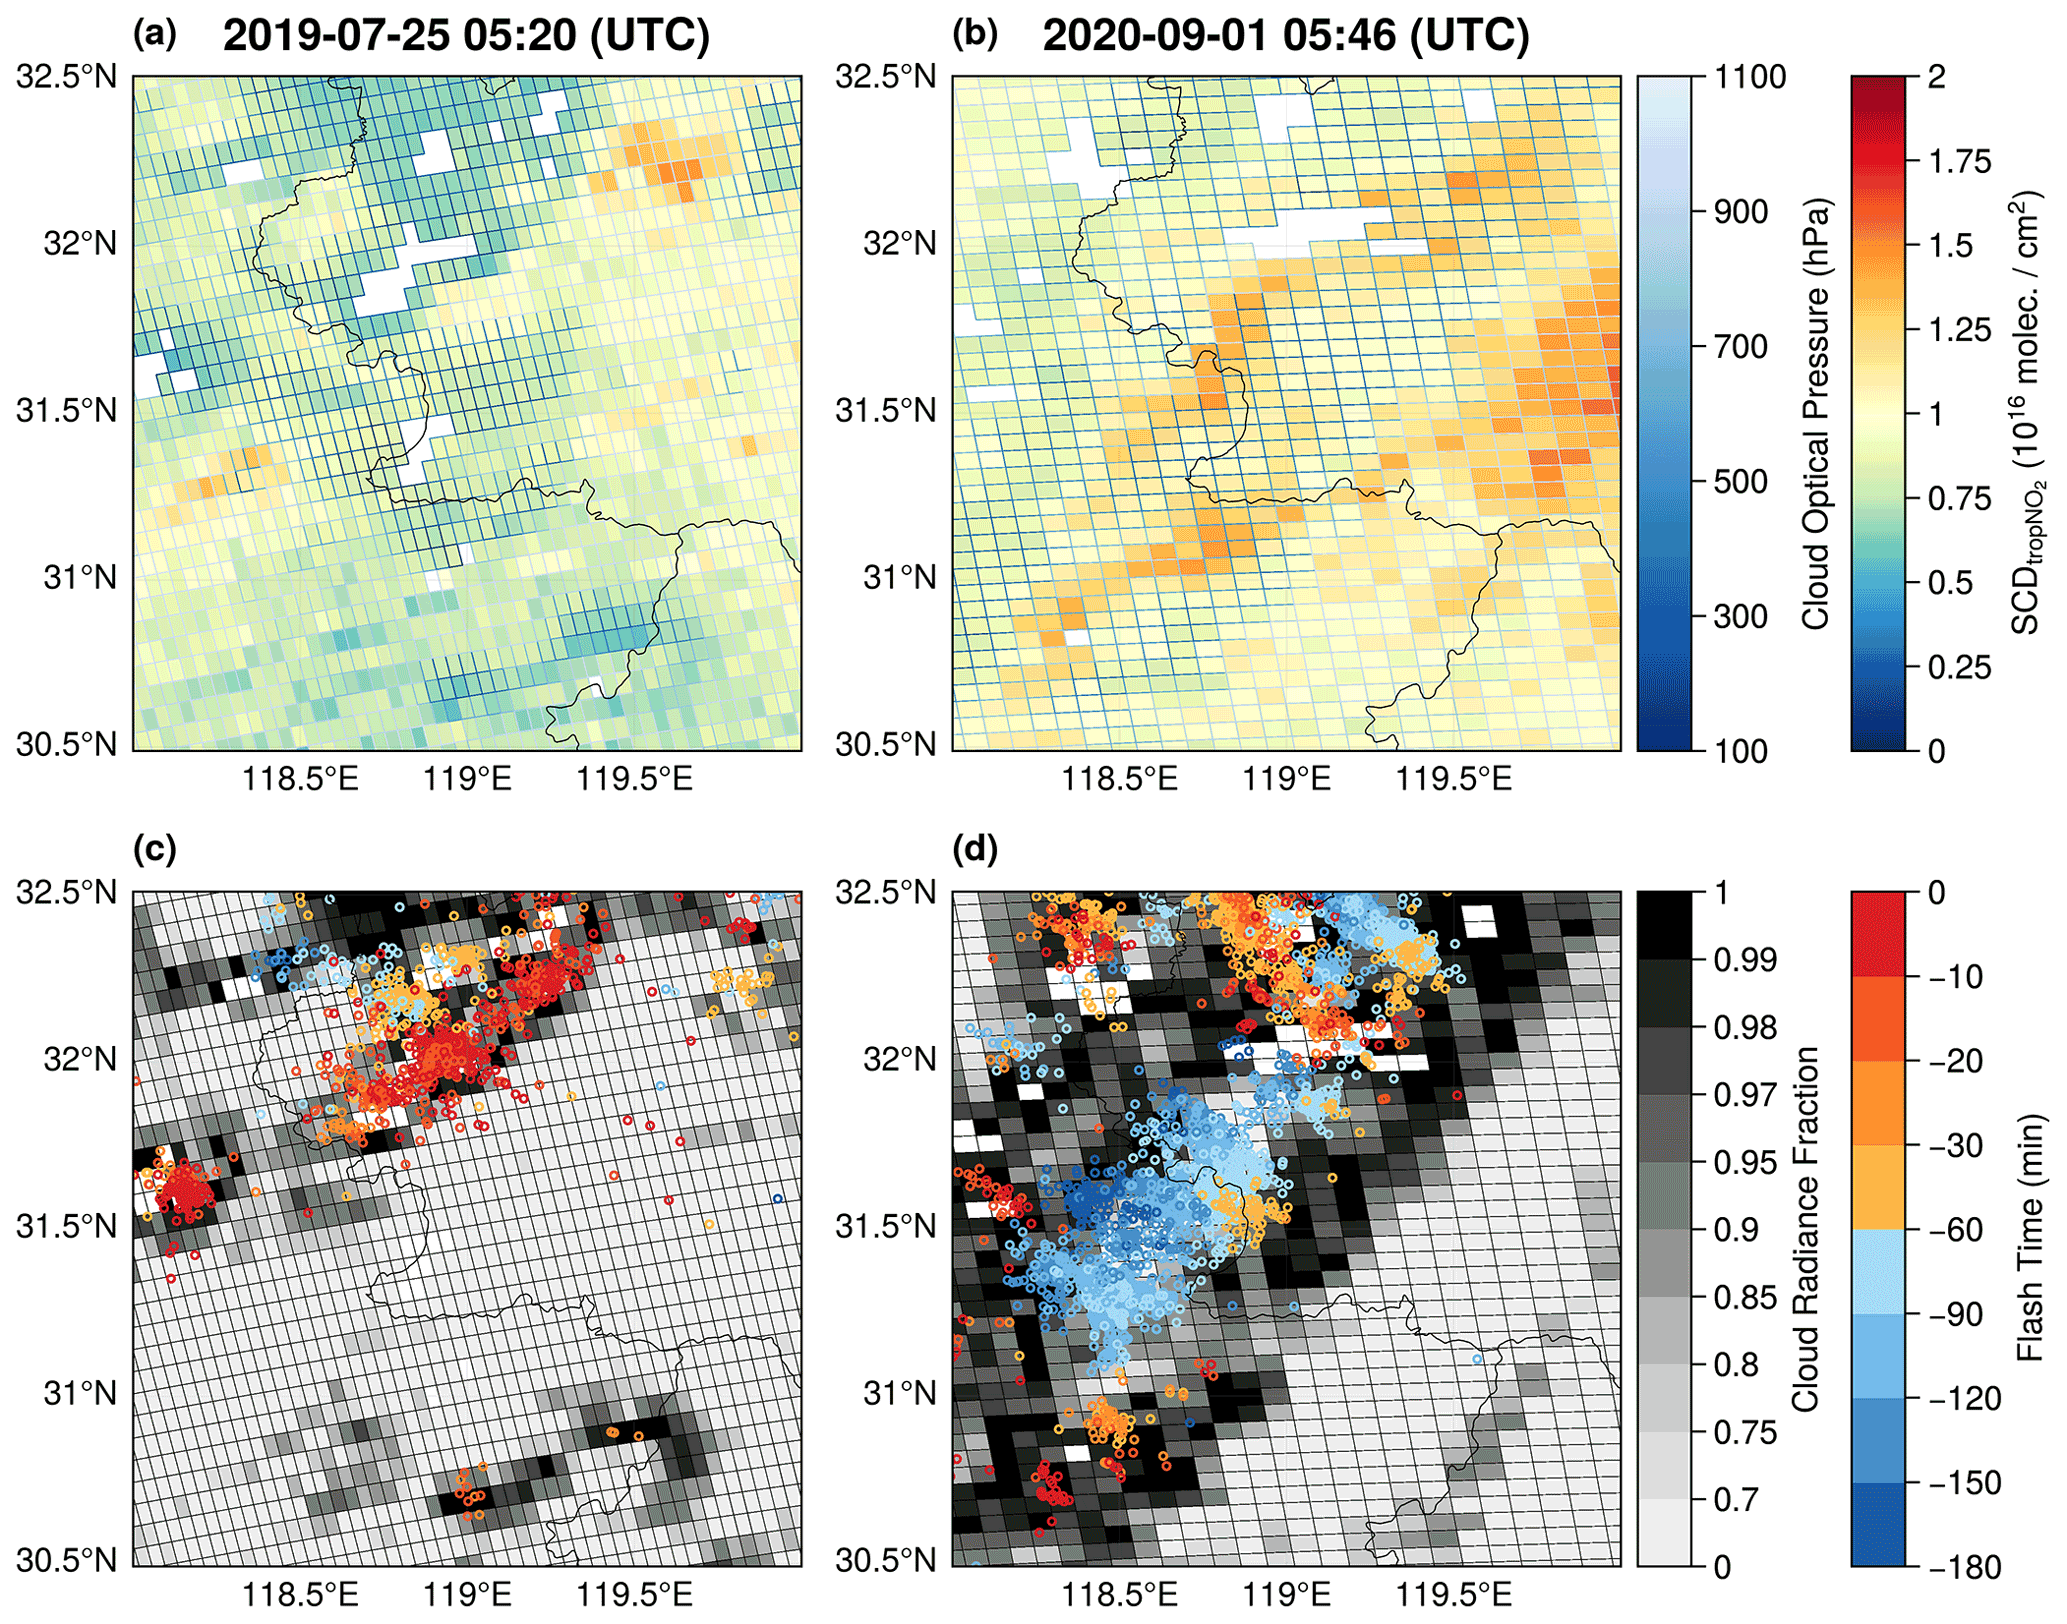
\includegraphics[width=12cm]{./figures/flash_scd.png}
    \caption{
    2019 年 7 月 25 日(左)和 2020 年 9 月 7 日(右)的个例。
    (a, b) 对流层 NO$_2$ 斜柱密度(SCD$_\textrm{tropNO$_2$}$,填充色)和云压(线条颜色)。
    这些白色网格单元代表缺失的 TROPOMI 数据,黑色实线为江苏省。
     (c, d) NO$_2$ 窗区中的云辐射分数和闪电。闪电的颜色取决于相对于TROPOMI过境的发生时间。\\
    Figure \ref{fig:flash_scd}. Events on 25 July 2019 (left) and 07 September 2020 (right).
    (a, b) The tropospheric NO$_2$ slant column density (SCD$_\textrm{tropNO$_2$}$, filled color) and cloud optical pressure (line color).
    These white grid cells stand for missing TROPOMI data.
    The solid black border is Jiangsu province.
    (c, d) The cloud radiance fraction in the NO$_2$ window and flashes whose color depends on the occurring time relative to the TROPOMI overpass time.
    }
    \label{fig:flash_scd}
\end{figure}


\begin{figure}[htbp]
    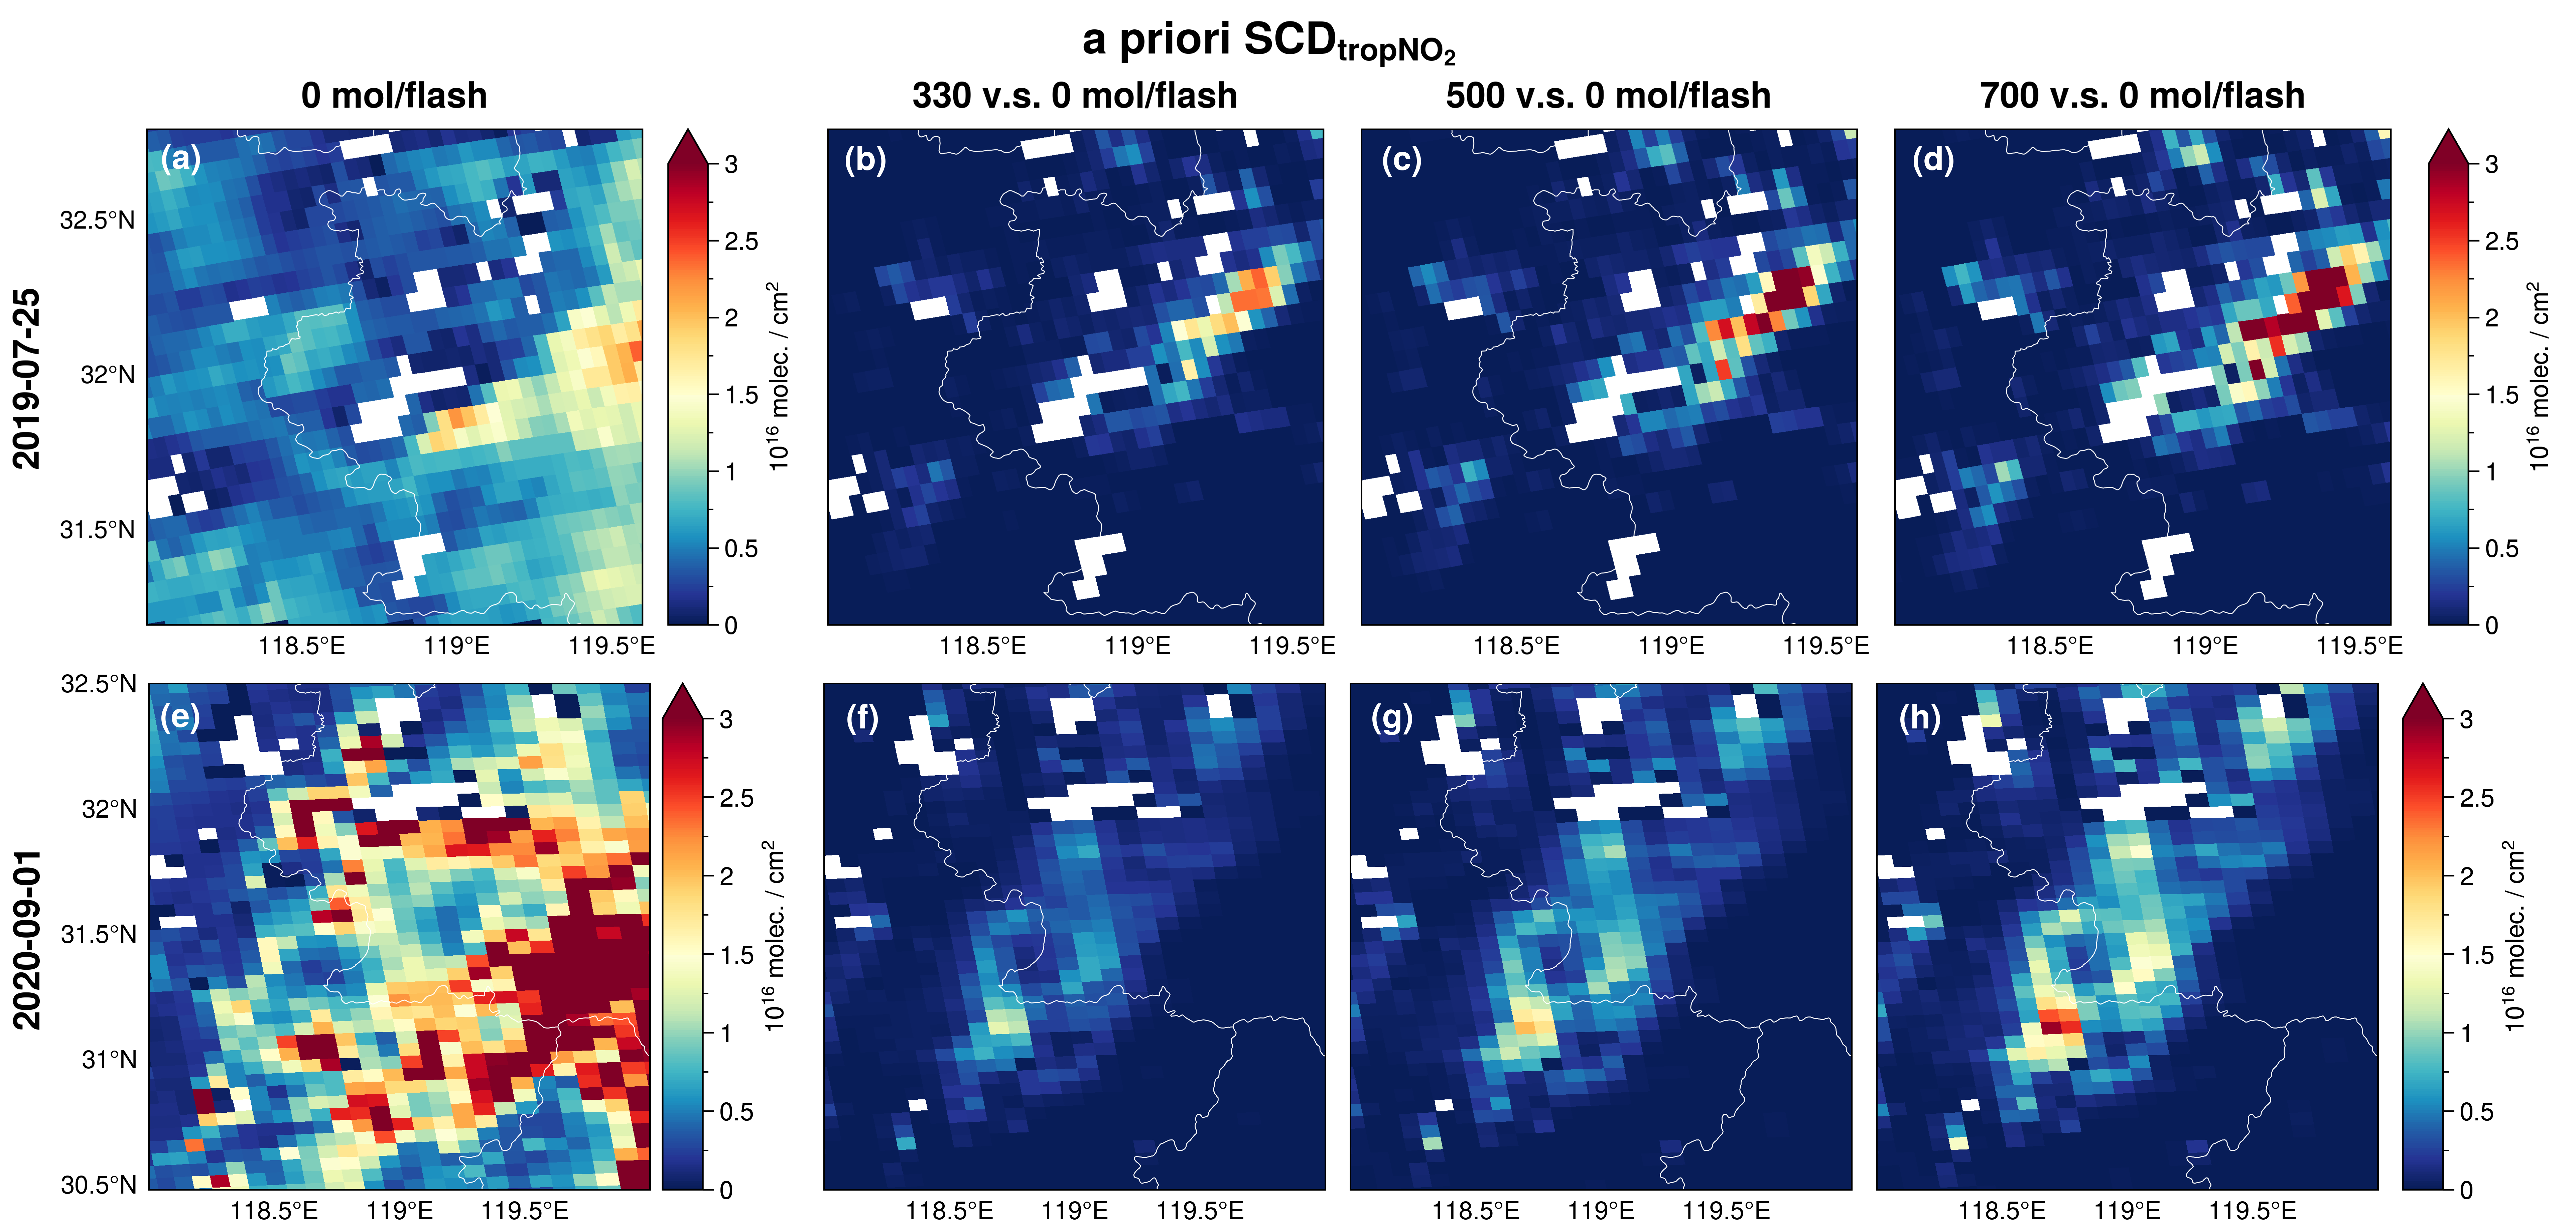
\includegraphics[width=17cm]{./figures/s5p_apriori_scd.png}
    \caption{使用不同闪电NO排放的WRF-Chem结果,重新计算得到的对流层NO$_2$斜柱密度 (SCD$_\textrm{tropNO$_2$}$):
    Figure \ref{fig:s5p_apriori_scd}. (a, e) 0 mol每闪电, (b, f ) 330 mol每闪电, (c, g) 500 mol每闪电 和 (d, h) 700 mol每闪电。\\
    The tropospheric NO$_2$ slant column density (SCD$_\textrm{tropNO$_2$}$) recalculated using the WRF-Chem results with different lightning NO settings: (a, e) 0 mol/flash, (b, f) 330 mol/flash, (c, g) 500 mol/flash and (d, h) 700 mol/flash.
    }
    \label{fig:s5p_apriori_scd}
\end{figure}


\begin{figure}[htbp]
    \centering
    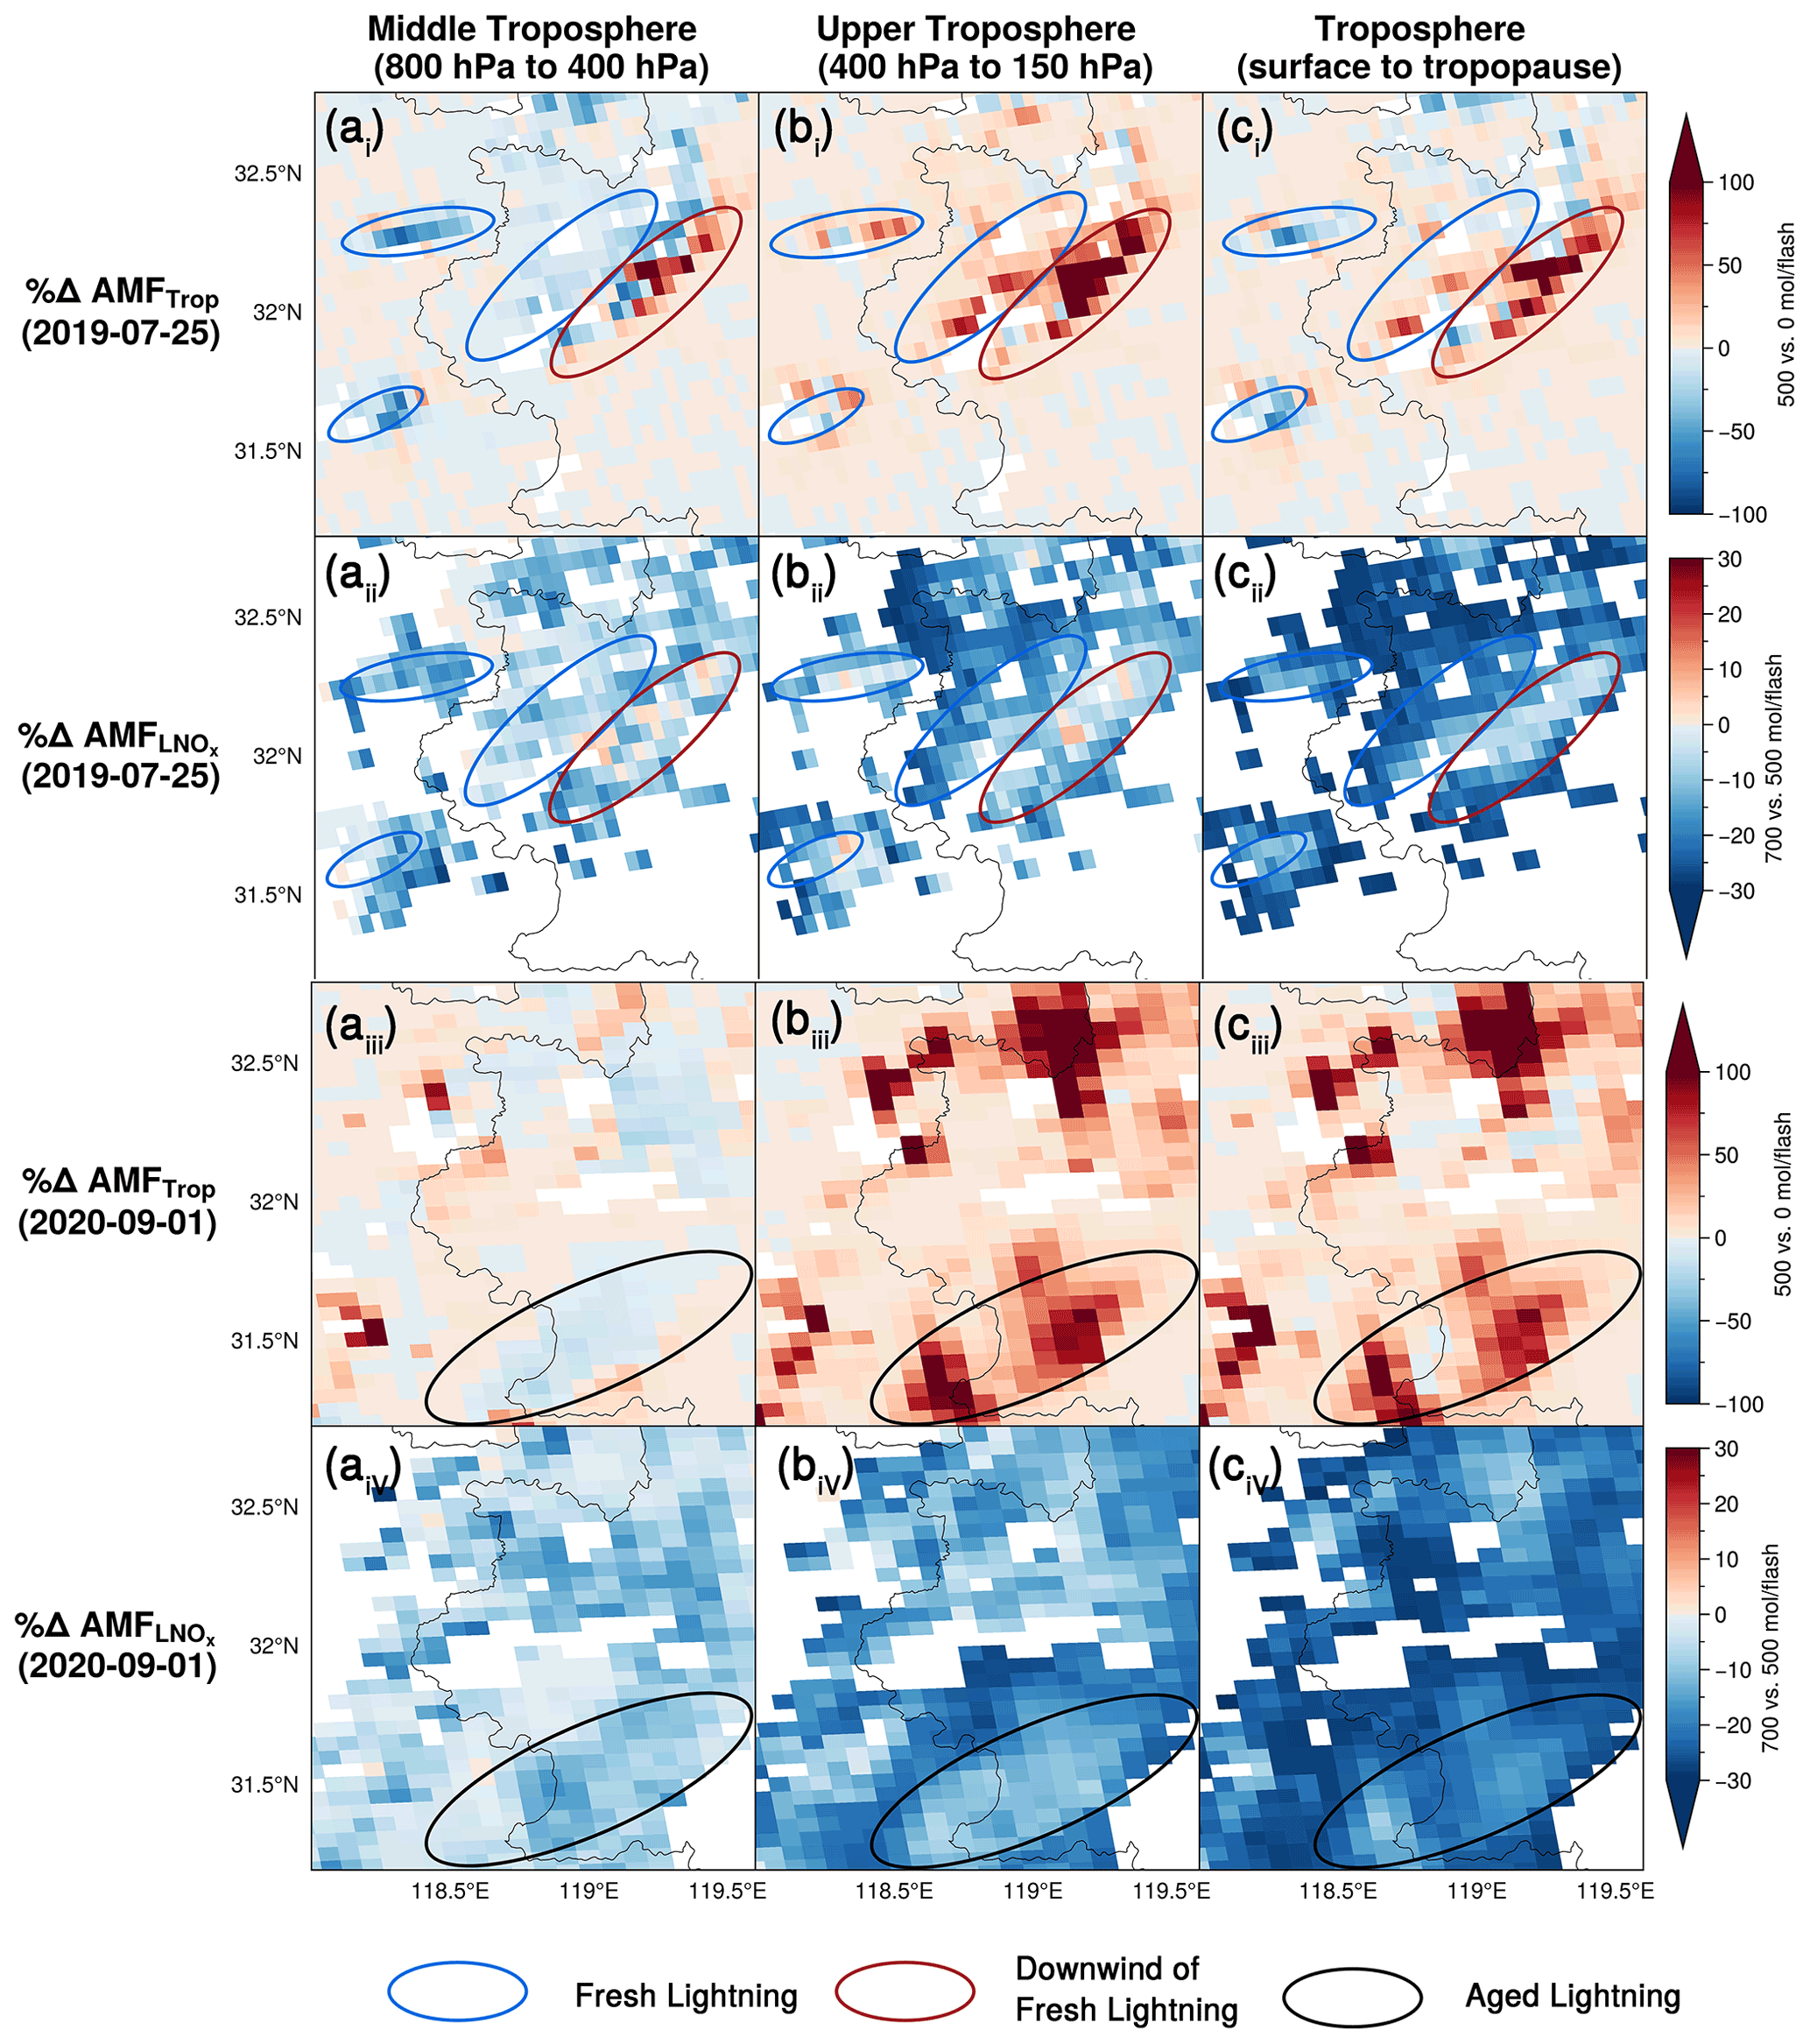
\includegraphics[width=12cm]{./figures/s5p_amf_diff.png}
    \caption{
    通过替换三层的NO$_2$先验廓线,得到的空气质量因子(AMF)百分比差异:三层具体为:对流层中层(左)、对流层上层(中)和整个对流层(右)。
     $\Delta$AMF$_\textrm{trop}$ 是 500 mol NO/闪电得到的AMF$_\textrm{trop}$ 与0 mol NO/闪电得到的AMF$_\textrm{trop}$之差。
     $\Delta$AMF$_\textrm{LNO$_x$}$ 是 500 mol NO/闪电得到的AMF$_\textrm{LNO$_x$}$ 与0 mol NO/闪电得到的AMF$_\textrm{LNO$_x$}$之差。
     标注了三个区域:新生闪电区(蓝色),闪电下风向(红色),和闪电老化区(黑色)。\\
    Figure \ref{fig:s5p_amf_diff}. The percent differences of AMFs by replacing the a priori NO$_2$ profiles at three layers:
    middle troposphere (left), upper troposphere (middle), and troposphere (right).
    $\Delta$AMF$_\textrm{trop}$ is the comparison of the AMF$_\textrm{trop}$ with 500 mol NO per flash relative to 0 mol NO per flash.
    $\Delta$AMF$_\textrm{LNO$_x$}$ is the comparison of the AMF$_\textrm{LNO$_x$}$ with 700 mol NO per flash relative to 500 mol NO per flash.
    Three regions are annotated: fresh lightning (blue),
    downwind of fresh lightning (red),
    and aged lightning (black).
    % Because of the quite large AMF$_\textrm{LNO$_x$}$ values in pixels with little lightning,
    % $\Delta$AMF$_\textrm{LNO$_x$}$ is shown over pixels where 0 $<$ AMF$_\textrm{LNO$_x$}$ $<$ 10.
    }
    \label{fig:s5p_amf_diff}
\end{figure}


\begin{figure}[htbp]
    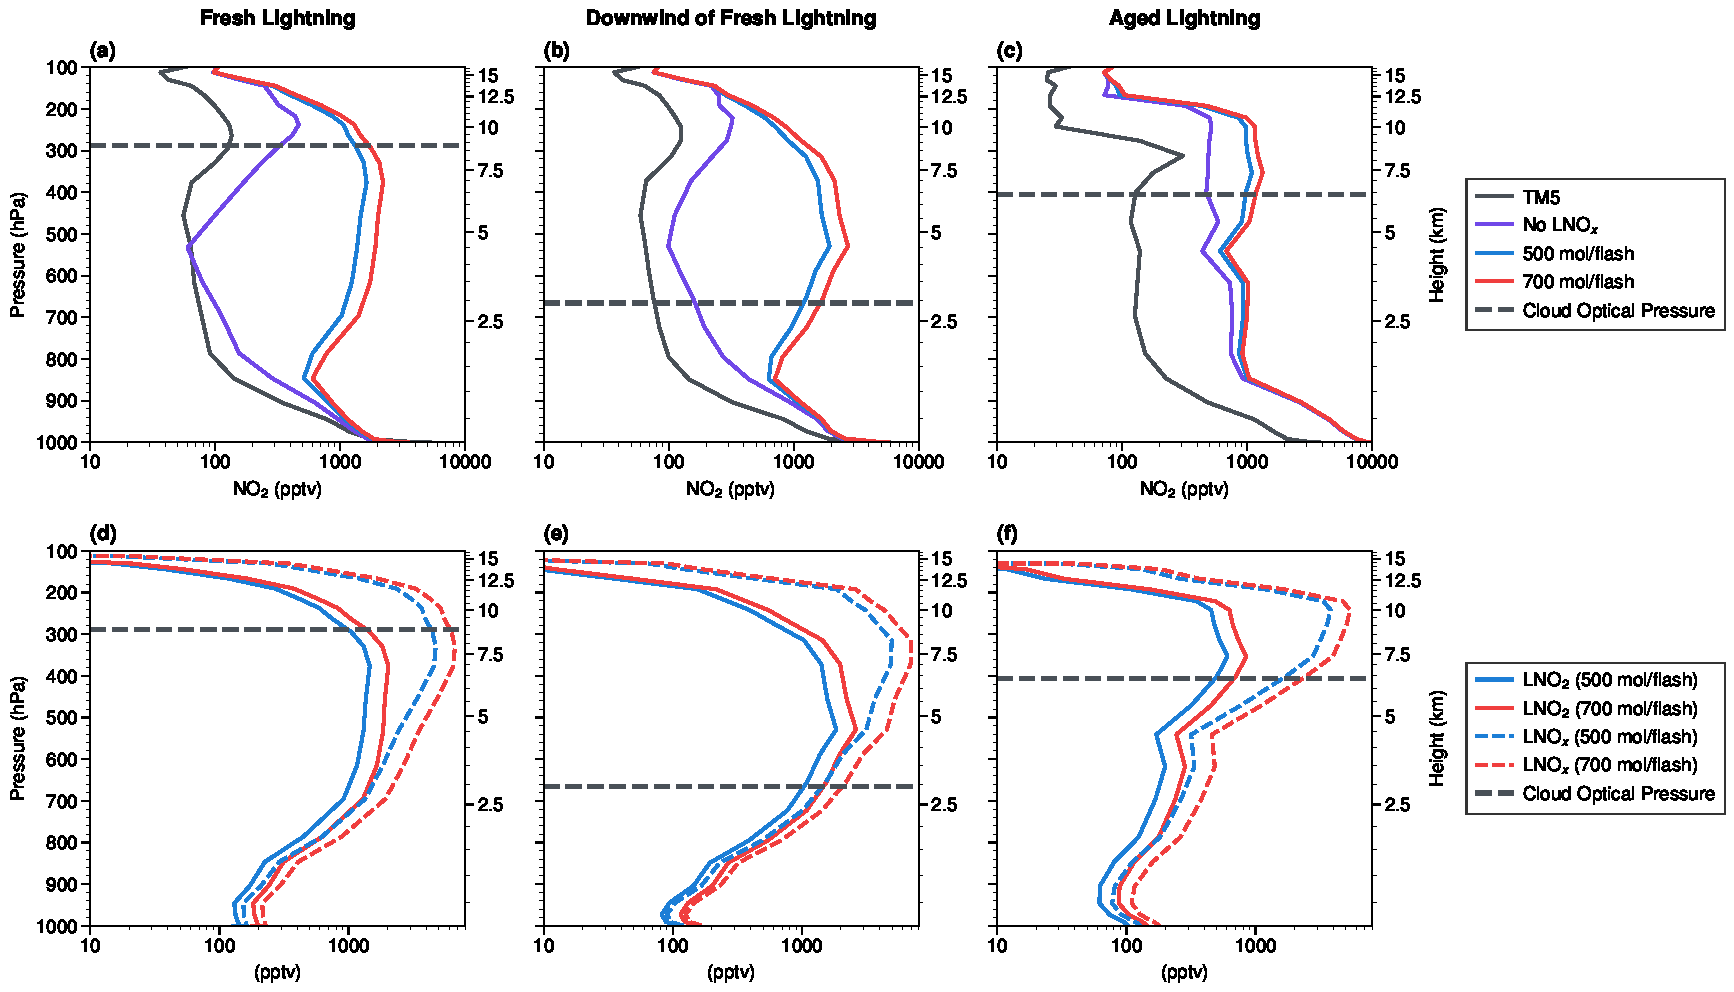
\includegraphics[width=17cm]{./figures/nox_profile.pdf}
    \caption{
    TROPOMI过境时,在不同闪电NO的排放条件下,三个区域(新生闪电区,闪电下风向,和闪电老化区)的各物质垂直廓线。
     (a--c) NO$_2$廓线与官方TM5先验NO$_2$廓线之间的比较。
     (d--f) 闪电 NO$_2$ 和 NO$_x$廓线。灰色虚线是TROPOMI探测到的云压。\\
     Figure \ref{fig:nox_profile}. Profiles with different lightning NO productions at TROPOMI overpass time over three regions (fresh lightning, downwind of fresh lightning, and aged lightning).
    (a--c) The NO$_2$ profiles compared with the official TM5 a priori NO$_2$ profile.
    (d--f) The lightning NO$_2$ and NO$_x$ profiles.
    The gray dashed line is the cloud optical pressure detected by TROPOMI.
    }
    \label{fig:nox_profile}
\end{figure}


\begin{figure}[htbp]
    \centering
    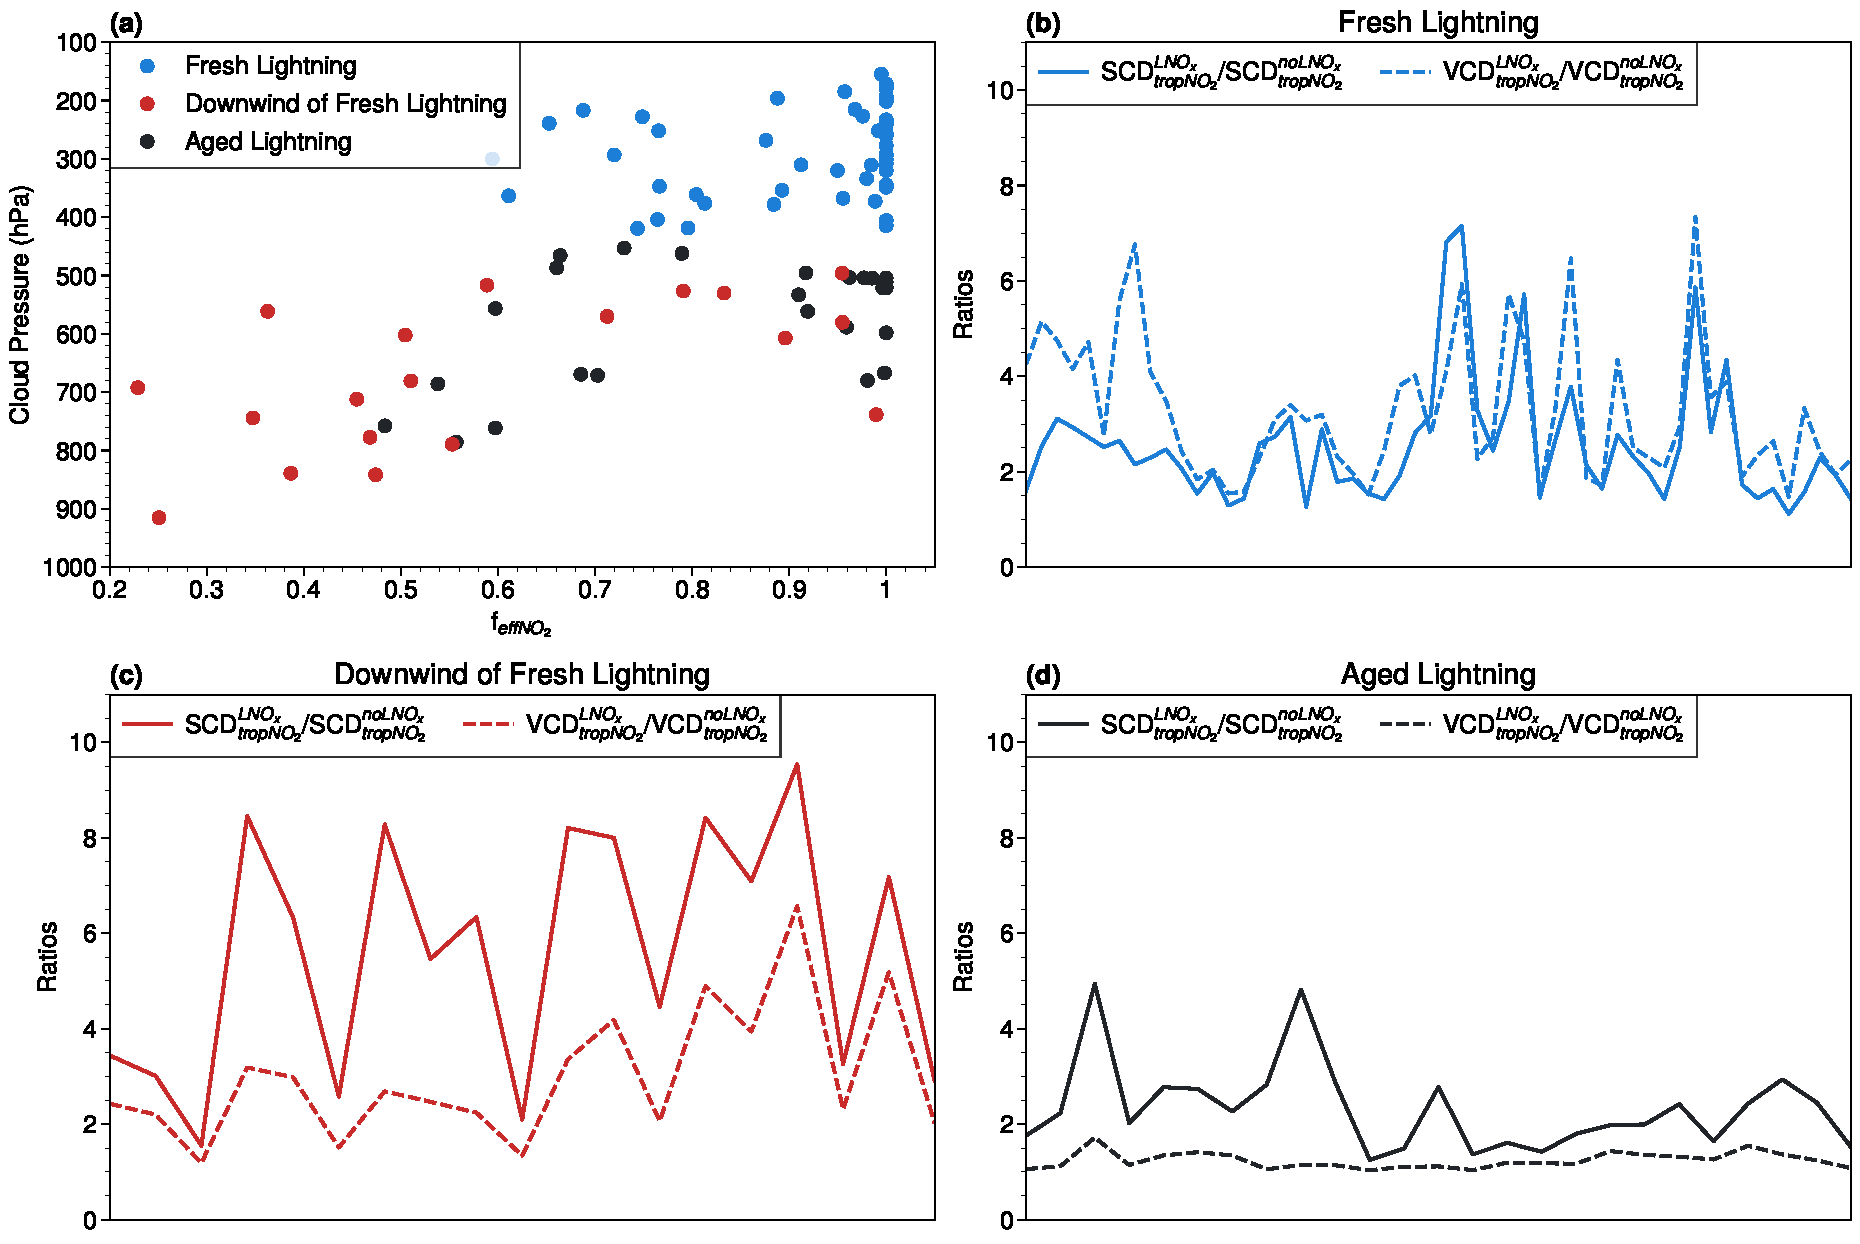
\includegraphics[width=14cm]{./figures/amf_contribution.pdf}
    \caption{
    (a) 图 \ref{fig:s5p_amf_diff} 中定义的三个区域(新生闪电区,闪电下风向,和闪电老化区)的云压和云辐射分数之间的关系。
     (b--d) 这三个区域的先验SCD$^{\textrm{LNO$_x$}}_{\textrm{tropNO$_2$}}$/SCD$^{\textrm{noLNO$_x$}}_{ \textrm{tropNO$_2$}}$和先验VCD$^{\textrm{LNO$_x$}}_{\textrm{tropNO$_2$}}$/VCD$^{\textrm{noLNO$_x$ }}_{\textrm{tropNO$_2$}}$。
     LNO$_x$的上标表示先验变量是通过开启LNO$_x$排放(每次闪光 500 mol NO)计算得到的,而上标为noLNO$_x$则代表未开启LNO$_x$排放。\\
     Figure \ref{fig:amf_contribution}. (a) The relationship between cloud pressure and cloud radiance fraction for three regions defined in Fig. \ref{fig:s5p_amf_diff}: fresh lightning region, downwind of fresh lightning, and aged lightning area.
    (b--d) The a priori SCD$^{\textrm{LNO$_x$}}_{\textrm{tropNO$_2$}}$/SCD$^{\textrm{noLNO$_x$}}_{\textrm{tropNO$_2$}}$ and a priori VCD$^{\textrm{LNO$_x$}}_{\textrm{tropNO$_2$}}$/VCD$^{\textrm{noLNO$_x$}}_{\textrm{tropNO$_2$}}$ of pixels in these three regions. The LNO$_x$ superscript indicates that the a priori variable is calculated with LNO$_x$ (500 mol NO per flash) and the noLNO$_x$ superscript is without LNO$_x$.
    }
    \label{fig:amf_contribution}
\end{figure}


\section{本章小结}

	%!TEX root = ../thesis.tex

\chapter{深对流对氮氧化物和臭氧垂直再分布的影响及机理}

\section{云切片算法} \label{sec:cloud-slicing}

前人研究表明,云切片方法(cloud-slicing)可用于计算云内O$_{\ch{3}}$和NO$_{\ch{2}}$的浓度,
该方法是计算O$_{\ch{3}}$总柱浓度的对流云微分法(CCD)的拓展\citep{Ziemke.1998,Ziemke.2001}。
简要来说,是通过线性拟合OMI或TROPOMI测得的云上NO$_{\ch{2}}$或O$_{\ch{3}}$柱浓度和$p_{cloud}$的斜率,从而得到NO$_{\ch{2}}$或O$_{\ch{3}}$的浓度,计算方法的框架见图\ref{fig:cloud-slicing_schematic}。

以TROPOMI的NO$_{\ch{2}}$产品为例,对于不同的$p_{cloud}$我们需要至少两个邻近的云上$V_{\ch{NO2}}$($V_{\ch{NO2Vis}}$,图\ref{fig:cloud-slicing_schematic}a),这两个测量的结果显示在图\ref{fig:cloud-slicing_schematic}b 中的$p_{cloud}$-VCD 坐标平面中。
两个气压层$p_1$ 和 $p_2$($p_1$ $<$ $p_2$)之间的$V_{\ch{NO2}}$
可以通过对$p_1$--$p_2$间的NO$_{\ch{2}}$体积混合比($VMR_{\ch{NO2}}$)进行积分得出:
\begin{equation} \label{eq:vmr_integ}
{VCD_{\ch{NO2}}}_{p_1}^{p_2}=\frac{R_{\ch{air}}}{k_Bg} \cdot \int_{p_1}^{p_2} VMR_{\ch{NO2}}(p) \mathrm{d} p
\end{equation}
其中 $R_{\ch{air}}$ 是气体常数,$k_B$ 是玻尔兹曼常数,$g$ 是重力加速度。
假设式(\ref{eq:vmr_integ})中 $p_1$ 到 $p_2$ 范围内的混合比恒定,此气压层内的平均$VMR_{\ch{NO2}}$由下式给出:
\begin{equation}
VMR_{\ch{NO2}} = \frac{\Delta V_{\ch{NO2Vis}}}{\Delta p} \frac{k_B g}{R_{air}}
\end{equation}

\begin{figure}[H]
\centering
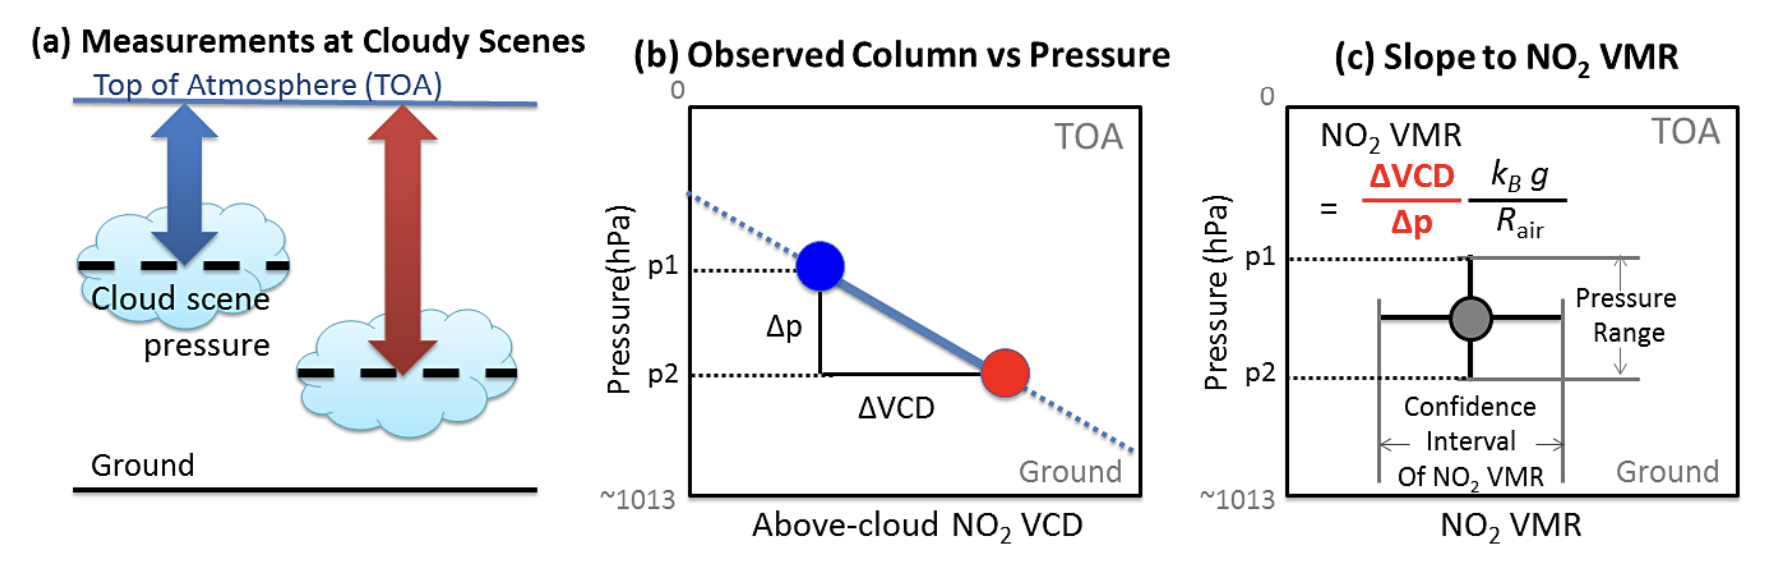
\includegraphics[width=\textwidth]{./figures/cloud-slicing_schematic.png}
\caption{云切片技术示意图(未按比例):(a)在不同云压条件下的两次云上NO$_{\ch{2}}$ 柱浓度测量(蓝色:云压低的柱浓度;红色:云压高的柱浓度);
(b)在气压柱坐标平面上显示的测量值; (c)NO$_{\ch{2}}$体积混合比(VMR)源自云上NO$_{\ch{2}}$垂直柱浓度(VCD)与云压的斜率,置信区间为水平误差条和气压范围为垂直误差条。[图片来源:\citet{Choi.2014}]\\
Figure \ref{fig:cloud-slicing_schematic}. Schematic view of the cloud-slicing technique (not to scale):
(a) two above-cloud NO$_{\ch{2}}$ column measurements at different cloud scene pressures (blue: column with lower scene pressure; and red: column with higher scene pressure);
(b) the measurements shown on a pressure-column coordinate plane;
(c) NO$_{\ch{2}}$ volume mixing ratios (VMR) derived from the slope of above-cloud NO$_{\ch{2}}$ vertical column densities (VCD) versus cloud scene pressure with confidence interval (horizontal error bar) and pressure range (vertical error bar). [Image source: \citet{Choi.2014}]
}
\label{fig:cloud-slicing_schematic}
\end{figure}

从这个关系式可以看出,TROPOMI云压范围内的$VMR_{\ch{NO2}}$与$V_{\ch{NO2Vis}}$和$p_{cloud}$的拟合斜率成正比(图\ref{fig:cloud-slicing_schematic}c)。
如果有两个以上的观测值,则可以从线性拟合中推导出$VMR_{\ch{NO2}}$的置信区间,
即图\ref{fig:cloud-slicing_schematic}c中$VMR_{\ch{NO2}}$的云压范围(垂直误差条)以及置信区间(水平误差条)。
在本文中,我们利用TROPOMI、TM5和MERRA2-GMI数据生成了各自在2019年6--8月对流层各高度区间内的平均$VMR_{\ch{NO2}}$,其中$p_{cloud}$位于以 330、450、570、670、770 和 870 hPa 为底的云压区间内。
由于TM5的NO$_{\ch{2}}$为TROPOMI NO$_{\ch{2}}$的附属产品,
故利用与下文TROPOMI相同的筛选条件进行数据筛选。
而MERRA2-GMI则选择当地时下午2点的模拟数据,计算每个云层区间内的最大云量,若某区间内的最大云量$>$ 0.4,则判断该区间为多云,并计算平均$VMR_{\ch{NO2}}$。

具体而言,$V_{\ch{NO2Vis}}$有两种计算方法:
1)基于近朗伯多云AMF假设,即具有较大总光学深度的散射云均匀分布在薄层上\citep{Choi.2014};
2)几何AMF,即$AMF_{\ch{geo}}$ = sec(SZA) + sec(VZA),其中 SZA 和 VZA 分别是太阳和视角天顶角\citep{Marais.2018,Marais.2021}。
由于对流层上层中NO$_{\ch{2}}$垂直分布的不确定性\citep{Travis.2016},我们使用$AMF_{\ch{geo}}$来计算云切片方法需要的$V_{\ch{NO2Vis}}$。
\citet{Choi.2014}的研究表明,该计算方法得到的$V_{\ch{NO2Vis}}$在对流层中层(650 hPa)最多比近朗伯多云AMF方法计算的结果高14\%。
因此,云切片算法中的$V_{\ch{NO2Vis}}$表达式如下:
\begin{equation} \label{eq:AMF_geo}
\begin{split}
V_{\ch{NO2Vis}} & = \frac{S_{\ch{NO2}}}{AMF_{\ch{geo}}} \\
             & = \frac{S_{\ch{total}}-(V_{\ch{strat}} \cdot AMF_{\ch{strat}})}{\sec (\mathrm{SZA})+\sec (\mathrm{VZA})}
\end{split}
\end{equation}
其中$S_{\ch{total}}$是总NO$_{\ch{2}}$斜柱浓度,$V_{\ch{strat}}$为平流层NO$_{\ch{2}}$垂直柱浓度,$AMF_{\ch{strat}}$为平流层空气质量分子。


虽然云切片方法无需知道具体的平流层NO$_{\ch{2}}$柱浓度即可推导出对流层的$VMR_{\ch{NO2}}$,但它依赖于以下假设和条件:
1)有相对大量的多云像素处于邻近位置,且这些像素具有足够的云压变化;
2)NO$_{\ch{2}}$在给定的云压和空间范围内,需在垂直和水平方向上充分混合;
3)平流层柱浓度在像素区域内保持不变;
4)计算得到的$VMR_{\ch{NO2}}$绝对量级仅与$V_{\ch{NO2Vis}}$具有一样的准确度,云压也可能会带来额外的不确定性。
因此,我们参考\citet{Marais.2021}设置了以下条件来获得有效的云切片结果。
首先将SZA $\geq$ 80$^{\circ}$ 和表面反照率 $\geq$  30\%的像素数据去除。
接着提取多云的像素[云辐射分数(CRF)$>$ 0.7],以最大限度地减少来自对流层下层的污染。
然后将每日的像素分配到1$^{\circ}$ $\times$ 1$^{\circ}$的网格中,保留满足云压具有足够大的变化范围[云压距离 $>$ 0.5*(最高云的气压 - 最低云的气压),且标准差$>$ 30 hPa]和充分混合的NO$_{\ch{2}}$(NO$_{\ch{2}}$ 垂直梯度 < 0.33 pptv hPa$^{-1}$)的像素。
若网格中像素个数超过10,则将得到的$VMR_{\ch{NO2}}$赋值到该日的网格点,最后可得到各高度的季节平均$VMR_{\ch{NO2}}$。

\section{痕量气体的垂直分布}

\subsection{二氧化氮}  \label{sec:no2_profile}


图\ref{fig:no2geo_tropomi}为TROPOMI观测的2019年中低纬度云上NO$_{\ch{2}}$柱浓度分布图,
气压区间分别为对流层顶--330 hPa、330--450 hPa、
450--570 hPa、570--670 hPa、670--770 hPa和770--870 hPa。
其中对流层顶--330 hPa和330--450 hPa的云上NO$_{\ch{2}}$高值区位于北美东北部、中国沿海地区、中国华北地区、墨西哥、
孟加拉国、尼泊尔、新德里、非洲中部和热带辐合带,
这些地区与图\ref{fig:no2_ltngcount}c中的闪电高值区相对应。
前人研究表明,中低纬LNO$_{\ch{2}}$的峰值分布在100--500 hPa之间\citep{Pickering.1988,Ott.2010,Luo.2017},
故对流层顶--450 hPa的云上NO$_{\ch{2}}$包含了LNO$_{\ch{2}}$的贡献。
然而TROPOMI的晴空NO$_{\ch{2}}$平均柱浓度产品显示这些地区属于NO$_{\ch{2}}$高污染区(图\ref{fig:no2_ltngcount}b),
所以云压处于对流层上层的NO$_{\ch{2}}$柱浓度也有来自深对流垂直输送的污染NO$_{\ch{2}}$。
中云(450--670 hPa)的云上NO$_{\ch{2}}$柱浓度有效数据更多,
其高值区包含了高云(对流层顶--450 hPa)的云上NO$_{\ch{2}}$柱浓度高值区。
其中污染NO$_{\ch{2}}$的贡献更为明显,与晴空NO$_{\ch{2}}$平均柱浓度产品分布更为接近,
如中国东部、欧洲和北美东北部的工业源以及非洲中部的生物质燃烧。
污染物排放在低云(670--870 hPa)的云上NO$_{\ch{2}}$柱浓度分布中最为明显,然而由于热带地区云顶较高,有效数据更少。



\begin{figure}[H]
    \centering
    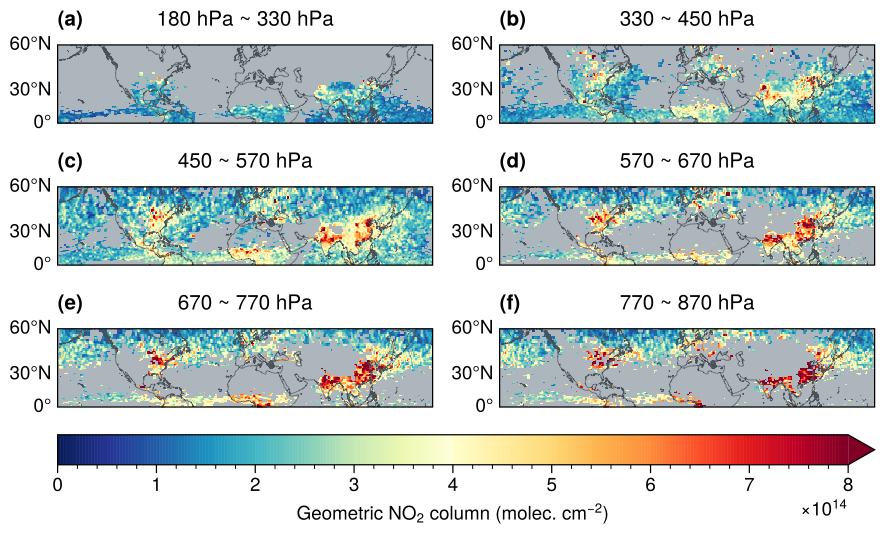
\includegraphics[width=0.9\textwidth]{./figures/no2geo_tropomi.png}
    \caption{
    2019年6--8月北半球中低纬度TROPOMI观测的云上NO$_{\ch{2}}$柱浓度分布图:
    高云[(a)对流层顶 --330 hPa 和(b)330--450 hPa],
    中云 [(c)450--570 hPa 和(d)570--670 hPa],
    及低云 [(e) 670--770 hPa 和(f)770--870 hPa]。 \\
    Figure \ref{fig:no2geo_tropomi}. NO$_{\ch{2}}$ above cloud at the middle-low latitudes for June--August in 2019:
    High clouds [(a) tropopause--330 hPa, (b) 330--450 hPa],
    middle clouds [(c) 450--570 hPa, (d) 570--670 hPa],
    and low clouds [(e) 670--770 hPa, (f) 770--870 hPa].
    }
    \label{fig:no2geo_tropomi}
\end{figure}

\begin{figure}[H]
    \centering
    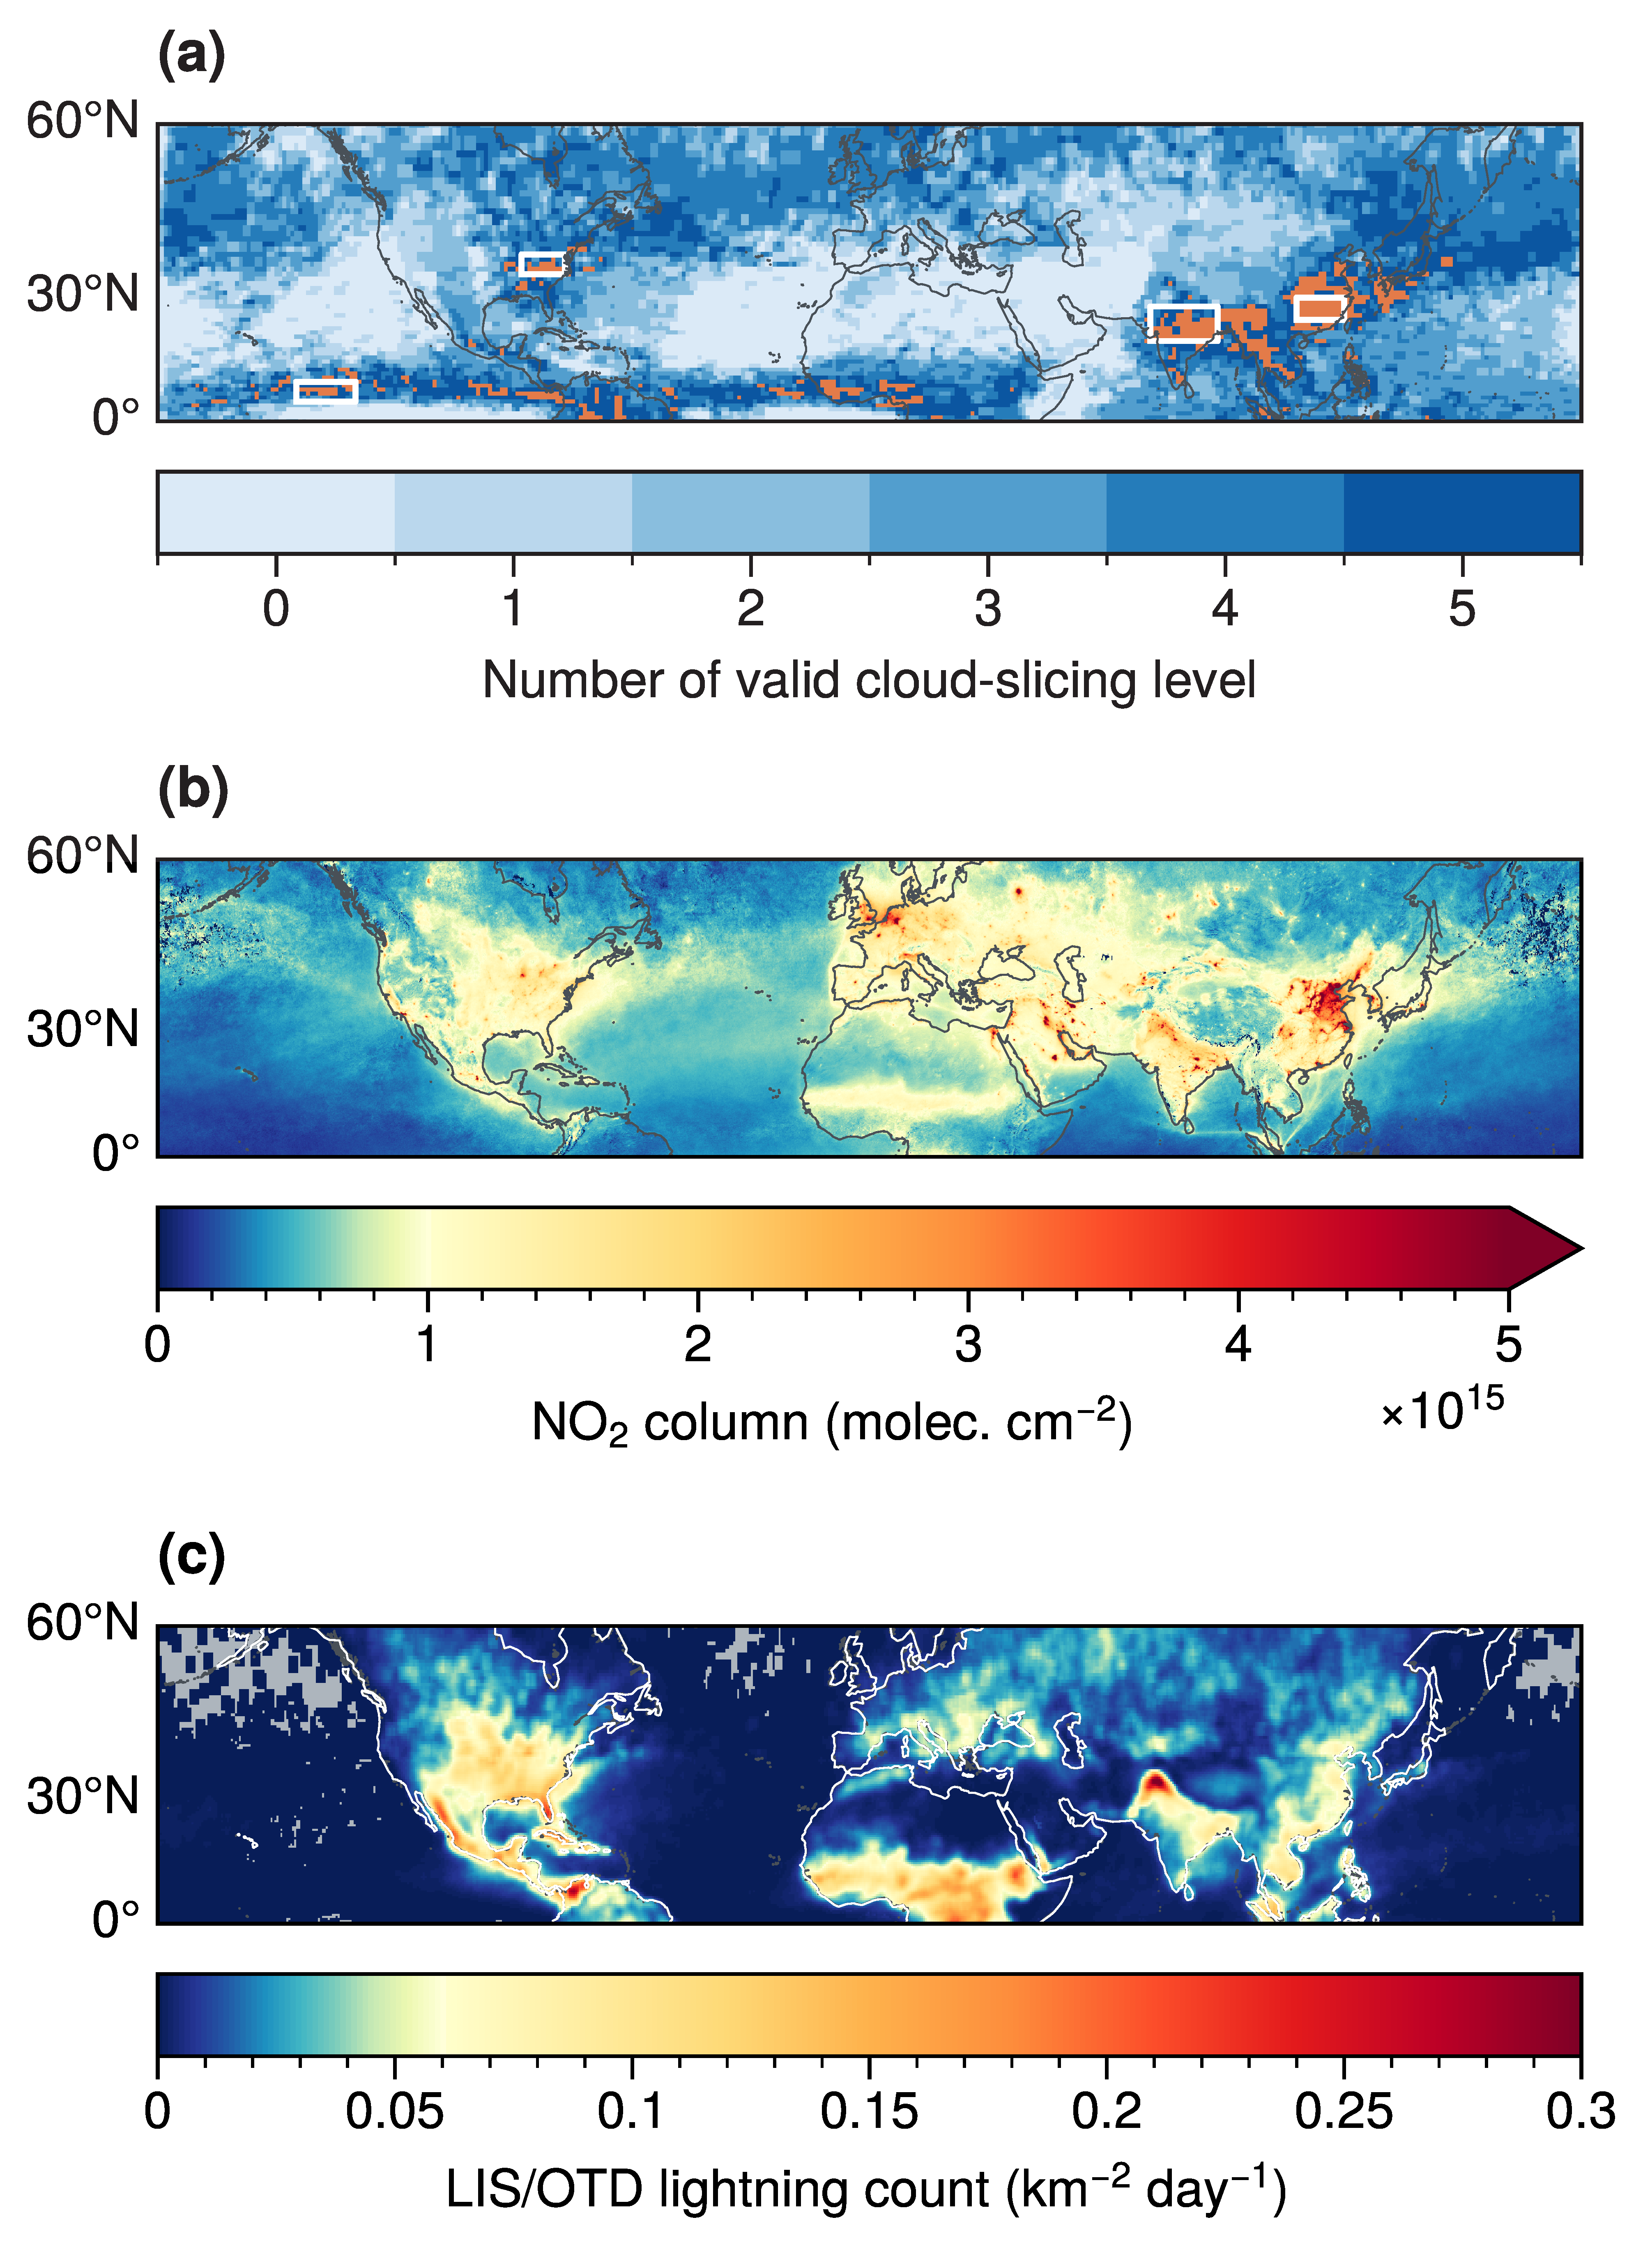
\includegraphics[width=0.7\textwidth]{./figures/no2_ltngcount.png}
    \caption{
    (a)云切片的总有效气压层数,层数$\leq$ 5为蓝色,= 6 为橙色,白色方框为NO$_{\ch{2}}$廓线选区(图\ref{fig:utno2_profile});
    (b)2019--2021年中低纬度夏季(6--8月)TROPOMI测得的NO$_{\ch{2}}$平均柱浓度;
    (c)1995--2014年中低纬度夏季(6--8月)LIS/OTD的闪电密度产品。 \\
    Figure \ref{fig:no2_ltngcount}. (a) Number of total valid cloud-slicing pressure levels.
    Grids with number of levels $\leq$ 5 and = 6 are filled in blue and orange, respectively.
    White rectangles are selections for NO$_{\ch{2}}$ profiles (Fig. \ref{fig:utno2_profile}).
    (b) The average TROPOMI NO$_{\ch{2}}$ column densities at the middle-low latitudes for June--August in 2019--2021.
    (c) The average LIS/OTD lightning flash rates at the middle-low latitudes for June--August in 1995--2014.
    }
    \label{fig:no2_ltngcount}
\end{figure}


利用\ref{sec:cloud-slicing}节的云切片算法,可进一步得到每层的NO$_{\ch{2}}$浓度,即NO$_{\ch{2}}$廓线。
图\ref{fig:utno2_tropomi}为2019年6--8月不同高度的NO$_{\ch{2}}$平均浓度。
与图\ref{fig:no2geo_tropomi}的云上NO$_{\ch{2}}$柱浓度不同,
高云处的NO$_{\ch{2}}$浓度(图\ref{fig:utno2_tropomi}a,b)高于中云(图\ref{fig:utno2_tropomi}c,d)。
其中陆地上对流层顶--330 hPa间的NO$_{\ch{2}}$浓度为330--450 hPa间的$\sim$1.2倍,为450--570 hPa间的$\sim$2倍,
而570 hPa以下(图\ref{fig:utno2_tropomi}d--f)陆地上的NO$_{\ch{2}}$浓度逐渐上升。
该现象与前人的模式模拟和飞机观测结果相符:LNO$_{\ch{2}}$在对流层上层占主导,
而人为污染NO$_{\ch{2}}$在对流层下层占主导\citep{Pickering.1996,Ott.2010,Laughner.2017}。


\begin{figure}[H]
    \centering
    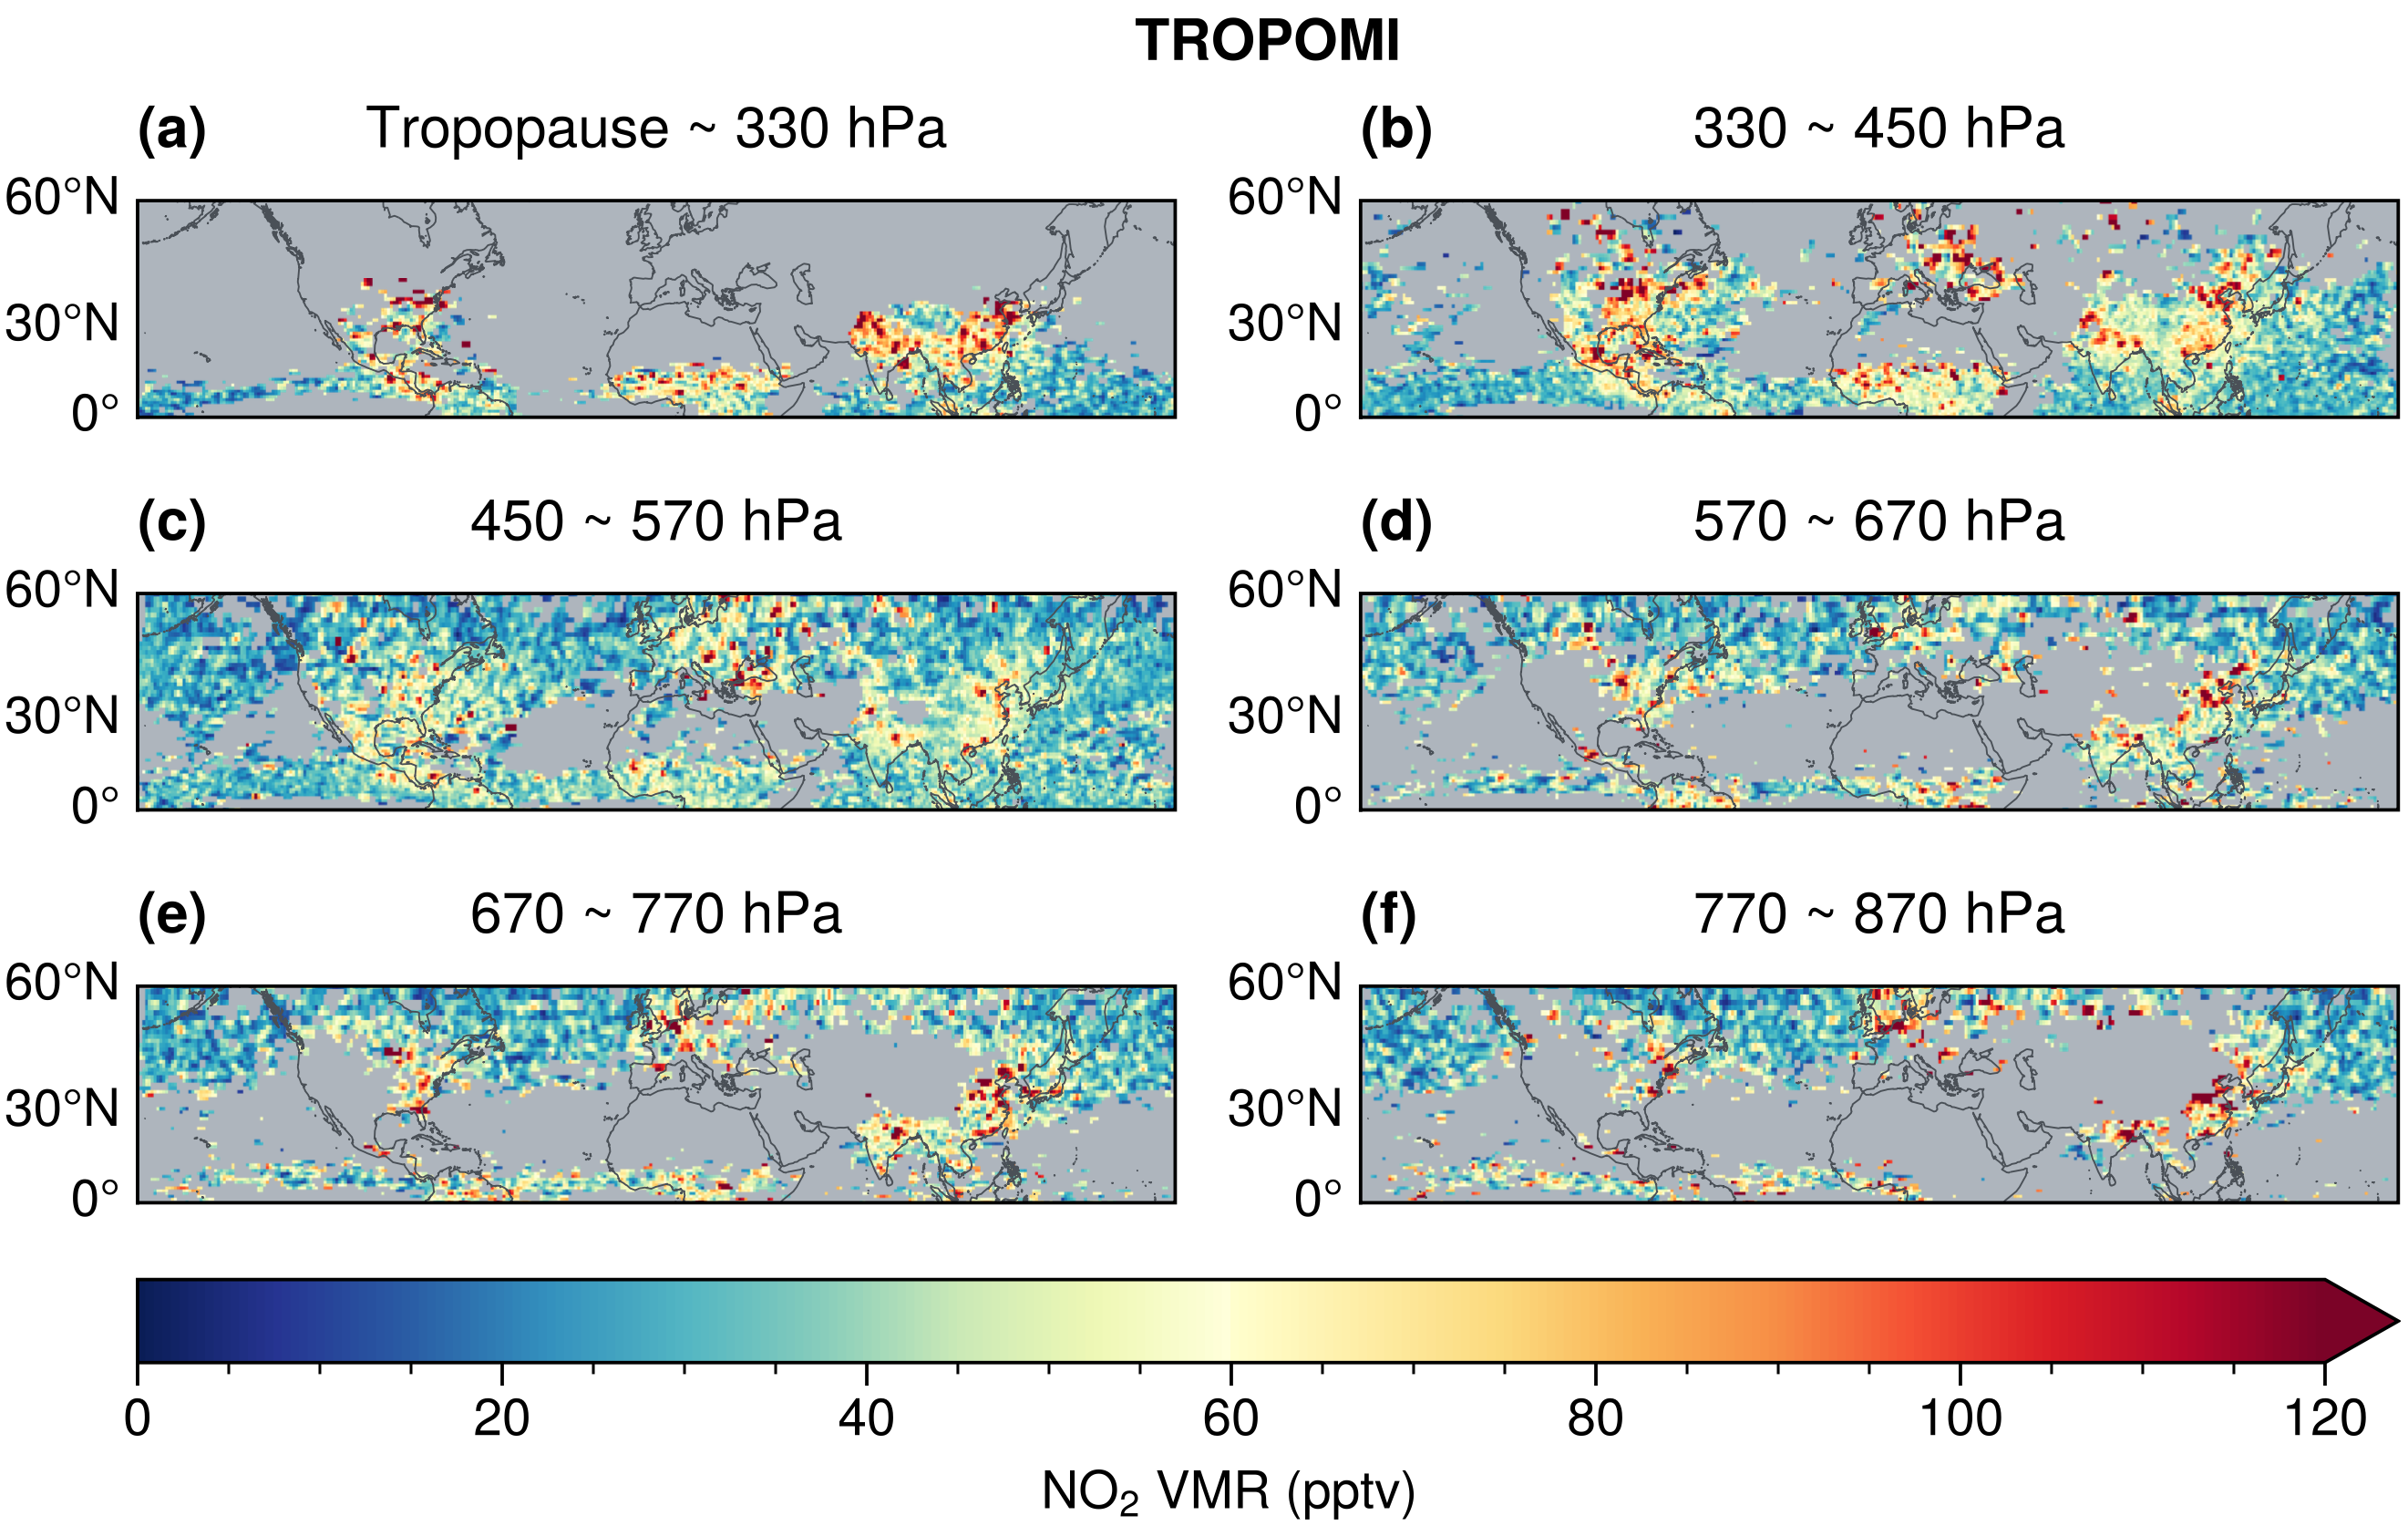
\includegraphics[width=0.9\textwidth]{./figures/utno2_tropomi.png}
    \caption{
    TROPOMI云切片算法所得的2019年6--8月北半球中低纬度NO$_{\ch{2}}$浓度分布图。 \\
    Figure \ref{fig:utno2_tropomi}. The NO$_{\ch{2}}$ vertical mixing ratios derived from the cloud-slicing results of TROPOMI NO$_{\ch{2}}$ observations at the northern middle-low latitudes for June--August in 2019.
    }
    \label{fig:utno2_tropomi}
\end{figure}

为了进一步分析LNO$_{\ch{2}}$在其中的作用,我们首先将各个高度层的TROPOMI观测结果与MERRA2-GMI的模式结果相比较,
接着选取TROPOMI云切片各层均有有效数据的区域,结合过境期间模拟的LNO$_{\ch{2}}$排放速率垂直分布进行廓线分析。
图\ref{fig:utno2_merra2}为2019年6--8月与TROPOMI对应的MERRA2-GMI NO$_{\ch{2}}$模拟结果,
% 由两者浓度之差(TROPOMI - MERRA2-GMI,图\ref{fig:utno2_delta})可知,无论位于陆地还是海洋,MERRA2-GMI较TROPOMI存在20--80 pptv的低估,
图\ref{fig:utno2_delta}为两者浓度之差(TROPOMI - MERRA2-GMI)的分布图。
其中海洋上的误差可能由TROPOMI NO$_{\ch{2}}$反演过程中低估的平流层NO$_{\ch{2}}$柱浓度或高估的辐射强度所导致\citep{VanGeffen.2020}。

具体而言,高云间的NO$_{\ch{2}}$正误差为28 $\pm$ 19 pptv,
% 即高云间MERRA2-GMI模拟的NO$_{\ch{2}}$比TROPOMI的观测值低25\%,
主要位于北美、东欧以及亚洲东部沿海(图\ref{fig:utno2_delta}a,b),
这意味着MERRA2-GMI全球模式中参数化对流垂直传输污染物的强度可能偏低。
而高云间的NO$_{\ch{2}}$负误差(-12 $\pm$ 11 pptv)位于美国中部、非洲中部以及青藏高原西南部。
美国中部和非洲中部的误差是由于MERRA2-GMI中的闪电参数化(对流层上层的向上云质量通量)高估了该区域的闪电总量,从而导致NO$_{\ch{2}}$浓度偏大\citep{Allen.2002,Allen.2010}。
由LIS/OTD闪电观测数据(图\ref{fig:no2_ltngcount}c)可知,
青藏高原西南部闪电强度较弱,故模式的高估主要应来自于亚洲夏季风的污染物输送。

中云的云切片结果有效范围最广,总体上来看TROPOMI和MERRA2-GMI之间误差较低(18 $\pm$ 17 pptv),
且两者具有相似的高值区分布:北美、东欧、印度以及中国华北地区,这些地区与污染NO$_{\ch{2}}$柱浓度高值区对应。
中云高度的NO$_{\ch{2}}$可能来源有对流输送的地表污染和污染的出流区,如中国华北地区的NO$_{\ch{2}}$高值传输至东部的黄海(其中一部分也来自于船舶排放)。
其中$>$ 40 pptv的正误差集中于南美洲北部、缅甸和泰国北部,由于这些地区地基NO$_{\ch{2}}$观测资料稀缺,
所以该误差应归因于卫星反演误差还是模式NO$_{\ch{x}}$排放源的不确定性,还有待进一步研究。
此外,中云的负误差结果在570--670 hPa更为明显(-10 $\pm$ 15 pptv),尤其是中国的华北地区,
考虑到MERRA2-GMI对流垂直输送强度较低,故使用的排放清单中NO$_{\ch{x}}$排放量可能过高\citep{Ziemke.2019}。

\begin{figure}[H]
    \centering
    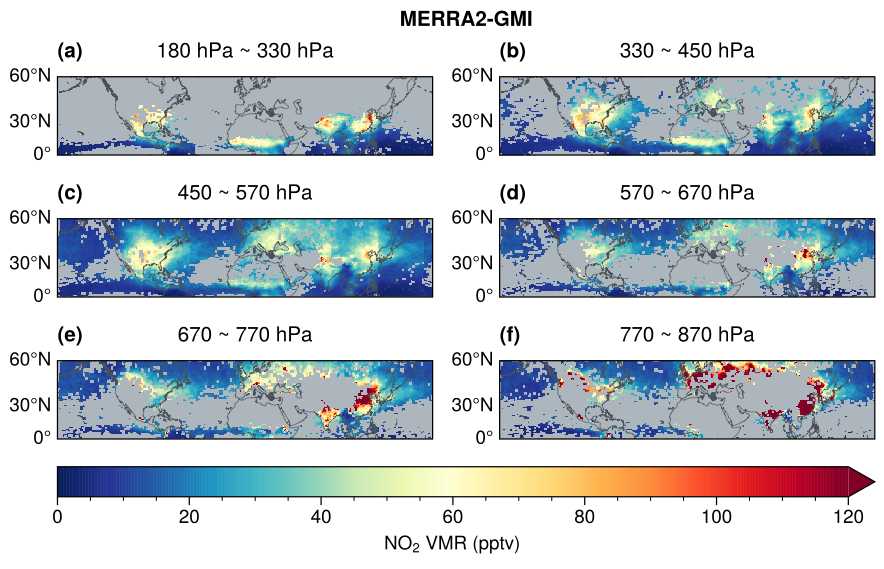
\includegraphics[width=0.9\textwidth]{./figures/utno2_merra2-gmi.png}
    \caption{
    同图\ref{fig:utno2_tropomi}但数据为MERRA2-GMI。 \\
    Figure \ref{fig:utno2_merra2}. Same as Fig. \ref{fig:utno2_tropomi} but for MERRA2-GMI.
    }
    \label{fig:utno2_merra2}
\end{figure}

低云的云切片NO$_{\ch{2}}$高值区与中云结果类似,
总体上来看TROPOMI和MERRA2-GMI之间误差较大(15 $\pm$ 50 pptv),
在中国东部和印度北部的负误差最为明显($<$-100 pptv)。
前人研究表明,本研究中所用的几何AMF(AMF$_{geo}$,式\ref{eq:AMF_geo})在低云和污染条件下可达可见AMF(AMF$_{Vis}$,式\ref{eq:AMF_NO2Vis})的两倍\citep{BelmonteRivas.2015},然而这不足以解释中国东部地区的模拟值为观测值的3--5倍。
因此,该差异反映了MERRA2-GMI使用的MACCity排放清单在中国东部未能及时更新。


\begin{figure}[H]
    \centering
    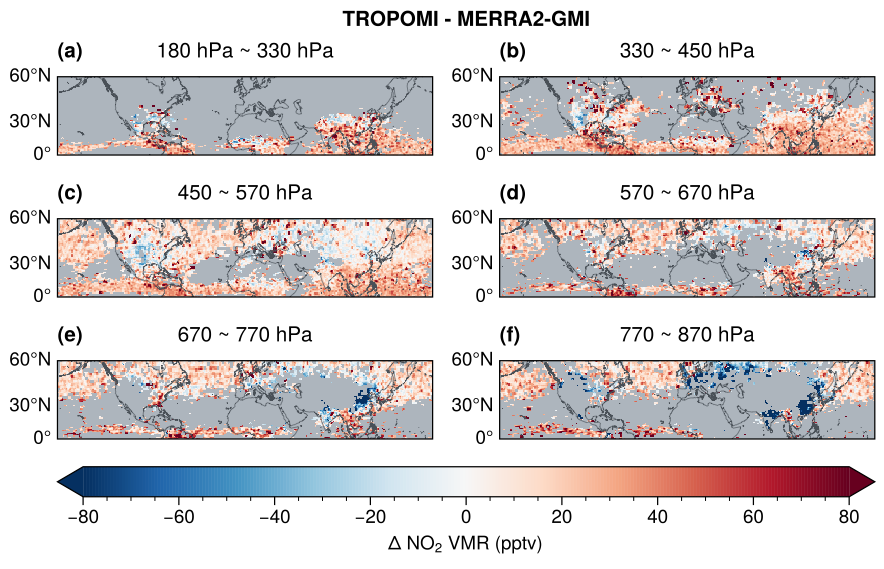
\includegraphics[width=0.9\textwidth]{./figures/utno2_delta.png}
    \caption{
    图\ref{fig:utno2_tropomi}与图\ref{fig:utno2_merra2}之差。 \\
    Figure \ref{fig:utno2_delta}. Differences between Fig. \ref{fig:utno2_tropomi} and Fig. \ref{fig:utno2_merra2}.
    }
    \label{fig:utno2_delta}
\end{figure}



除了各层NO$_{\ch{2}}$浓度的地理分布之外,我们选取了区域内云切片有效层数为6层的格点
(分别位于中国南部、印度中部、美国东南部以及太平洋,图\ref{fig:no2_ltngcount}a),
进行TM5、MERRA2-GMI和TROPOMI的廓线对比分析,
其中TM5的NO$_{\ch{2}}$廓线为TROPOMI官方产品使用的TM5全球模式先验廓线(包含TROPOMI同化)。
由于TROPOMI在太平洋清洁地区的高估,我们将云切片结果进行校正,即除以其与MERRA2-GMI和TROPOMI比例的平均值。
如图\ref{fig:utno2_profile}所示,太平洋清洁地区NO$_{\ch{2}}$在对流层各层浓度分布均一(2.5--12.5 pptv),
中国南部和印度中部低层NO$_{\ch{2}}$污染浓度高(200--300 pptv),而美国东南部低层NO$_{\ch{2}}$浓度为50--100 pptv。
由于污染地区对流层低层TROPOMI NO$_{\ch{2}}$浓度存在与图\ref{fig:utno2_delta}中类似的低估,故只比较三者在对流层中上层的NO$_{\ch{2}}$浓度大小。


\begin{figure}[H]
    \centering
    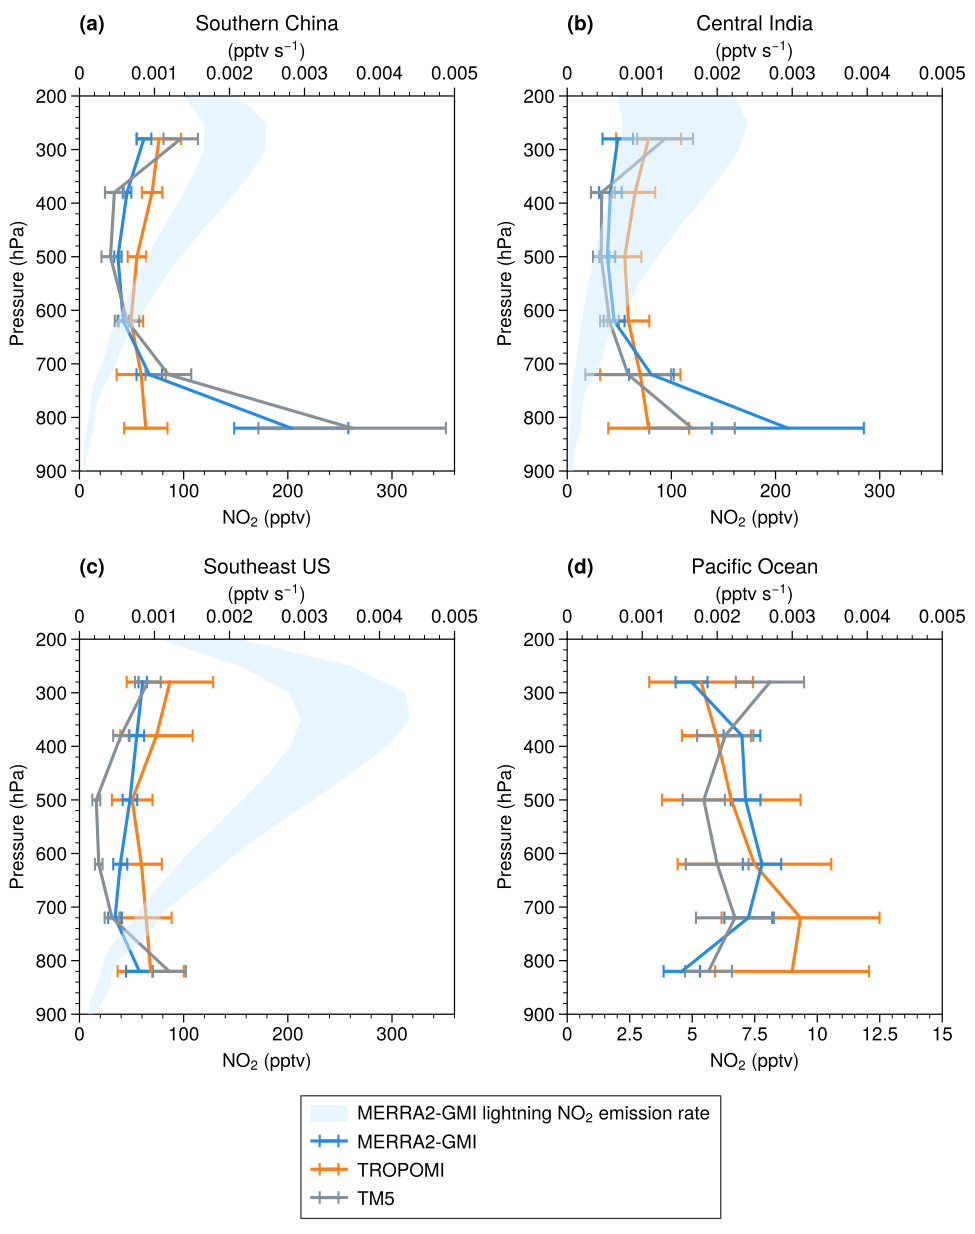
\includegraphics[width=0.9\textwidth]{./figures/utno2_profile.png}
    \caption{
    TM5(灰色)、MERRA2-GMI(蓝色)以及TROPOMI云切片算法(橙色)所得到的区域平均NO$_{\ch{2}}$廓线:
    (a)中国南部、(b)印度中部、(c)美国东南部、(d)太平洋(区域示意图见图\ref{fig:no2_ltngcount}a)。
    浅蓝色填充部分为下午地方时2点的MERRA2-GMI闪电NO$_{\ch{2}}$排放速率,
    其中廓线的误差棒和填充范围为平均值$\pm$标准差。\\
    Figure \ref{fig:utno2_profile}. Regional average NO$_{\ch{2}}$ profiles obtained by TM5 (gray), MERRA2-GMI (blue), and TROPOMI cloud slice algorithm (orange).
    (a) southern China, (b) central India, (c) southeastern United States, and (d) Pacific Ocean
    (Definitions of region are shown in Fig. \ref{fig:no2_ltngcount}a).
    The light blue filled part is the MERRA2-GMI lightning NO$_{\ch{2}}$ emission rate at local 2 p.m.,
    where the error bars and filled ranges of the profiles are the mean values $\pm$ standard deviations.
    }
    \label{fig:utno2_profile}
\end{figure}


对于中国南部、印度中部和美国东南部,NO$_{\ch{2}}$廓线呈“C”形:NO$_{\ch{2}}$首先随高度而下降,
在500--600 hPa存在转折点,进而浓度上升,在对流层顶--300 hPa达到峰值($\sim$80 pptv)。
总体来看,对流层中上层MERRA2-GMI和TM5的NO$_{\ch{2}}$浓度相近,但均比TROPOMI的结果低,
表明模式中LNO$_{\ch{2}}$或对流输送的污染NO$_{\ch{2}}$存在低估,与前人的飞机探测和模式结果相符\citep{Laughner.2019a}。
具体而言,由于TM5的同化仅包含云上的信息,TM5的中上层拐点梯度更大,
其在对流层顶--330 hPa和330--450 hPa区间的NO$_{\ch{2}}$浓度比TROPOMI的观测结果分别低10\%和50\%,
而MERRA2-GMI结果较TROPMI的结果低30\%。
此外,MERRA2-GMI在美国东南部的LNO$_{\ch{2}}$排放速率为中国南部或印度中部的两倍,最上层的峰值浓度与TM5一致,
不同之处是浓度拐点降为700 hPa,该高度低于TM5和TROPOMI的500 hPa,
可能原因是MERRA2-GMI的美国东南部LNO$_{\ch{2}}$排放廓线在对流层中低层权重过高。
总之,TROPOMI的观测结果和MERRA2-GMI/TM5的模拟结果在对流层中上层存在显著的一致性,
局部的差异表明云切片方法可以用来检验模式的对流垂直输送和水平输送能力、使用的排放源清单以及LNO$_{\ch{x}}$的产量和分布。


\subsection{臭氧} \label{sec:o3_profile}

如图\ref{fig:uto3_tropomi}所示,云切片方法可得到2019年6--8月中低纬度对流云不同高度O$_{\ch{3}}$的平均浓度,
其有效范围比NO$_{\ch{2}}$的云切片结果(图\ref{fig:utno2_tropomi})更广,
尤其是在中云和高云条件下的中纬度地区(图\ref{fig:uto3_tropomi}b--d)。
这是由于TROPOMI的O$_{\ch{3}}$二级产品中云分数为光学云识别算法(OCRA)云分数,而NO$_{\ch{2}}$二级产品中使用从氧气A波段版本S(FRESCO-S)中快速检索云的方案。

总体来看,高云处的O$_{\ch{3}}$浓度(图\ref{fig:uto3_tropomi}a--b)高于中云(图\ref{fig:uto3_tropomi}c--d),
其中对流层顶--330 hPa间的O$_{\ch{3}}$为330--450 hPa间的$\sim$1.5倍,为450--570 hPa间的$\sim$2倍。
对于热带地区,非洲中部(20$^{\circ}$ W--50$^{\circ}$ E,0--20$^{\circ}$ N)的O$_{\ch{3}}$浓度比同纬度地区的O$_{\ch{3}}$浓度高,尤其是在中云和高云条件下可高出40--48\%,该现象与\citet{Cooper.2013}研究中215 hPa高度MLS的O$_{\ch{3}}$观测结果相符。
他们的研究指出,低O$_{\ch{3}}$事件经常发生在热带西太平洋,很少发生在热带其他地区,
而热带海洋区域在低O$_{\ch{3}}$事件和高云的频率之间存在一致的空间特征,表明这些事件来自于对流。
虽然非洲中部也是强对流频发地区,但生物质燃烧导致陆地边界层O$_{\ch{3}}$浓度往往高于海洋\citep{Thompson.2001,Anderson.2016},因此深对流产生较少的低O$_{\ch{3}}$事件。

\begin{figure}[H]
    \centering
    \includegraphics[width=0.95\textwidth]{./figures/uto3_tropomi.png}
    \caption{
    TROPOMI云切片算法所得的2019年6--8月北半球中低纬度O$_{\ch{3}}$浓度分布图。 \\
    Figure \ref{fig:uto3_tropomi}. The O$_{\ch{3}}$ vertical mixing ratios derived from the cloud-slicing results of TROPOMI O$_{\ch{3}}$ observations at the northern middle-low latitudes for June--August in 2019.
    }
    \label{fig:uto3_tropomi}
\end{figure}

为了进一步利用MERRA2-GMI的模式结果分析动力输送和化学反应在其中的作用,我们首先将各个高度的MERRA2-GMI模式结果与TROPOMI观测数据相比较。
图\ref{fig:uto3_merra2}为2019年6--8月与TROPOMI对应的MERRA2-GMI O$_{\ch{3}}$模拟结果,
图\ref{fig:uto3_delta}为TROPOMI与MERRA2-GMI在各层的结果之差($\Delta$ O$_{\ch{3}}$)。
总体上,非洲中部的$\Delta$ O$_{\ch{3}}$在中云和高云条件下为负(-23 $\pm$ 11 pptv,图\ref{fig:uto3_delta}a--d),
中纬度陆地地区的$\Delta$ O$_{\ch{3}}$在高云条件下为正(20 $\pm$ 15 pptv,图\ref{fig:uto3_delta}b)。
此外,$\Delta$ NO$_{\ch{2}}$(图\ref{fig:utno2_tropomi})和$\Delta$ O$_{\ch{3}}$(图\ref{fig:uto3_delta})的对比显示,
尽管中云和高云条件下NO$_{\ch{2}}$在大部分陆地地区被高估,但是O$_{\ch{3}}$却被低估。
\citet{Pickering.1990}于美国中南部清洁地区的研究显示,11 km处的LNO峰值排放导致该高度层为VOC控制区。
由于本研究全球模式中除化学反应外,动力输送也存在偏差,故不能确定是否为VOC控制区,有待将来进一步的研究。
低云条件下云切片算法低估O$_{\ch{3}}$的现象,也反映了AMF$_{\ch{geo}}$在低云和污染条件下的高估\citep{BelmonteRivas.2015}。


\begin{figure}[H]
    \centering
    \includegraphics[width=0.9\textwidth]{./figures/uto3_merra2-gmi.png}
    \caption{
    同图\ref{fig:uto3_tropomi}但数据为MERRA2-GMI。 \\
    Figure \ref{fig:uto3_merra2}. Same as Fig. \ref{fig:uto3_tropomi} but for MERRA2-GMI.
    }
    \label{fig:uto3_merra2}
\end{figure}


\begin{figure}[H]
    \centering
    \includegraphics[width=0.9\textwidth]{./figures/uto3_delta.png}
    \caption{
    图\ref{fig:uto3_tropomi}与图\ref{fig:uto3_merra2}之差。 \\
    Figure \ref{fig:uto3_delta}. Differences between Fig. \ref{fig:uto3_tropomi} and Fig. \ref{fig:uto3_merra2}.
    }
    \label{fig:uto3_delta}
\end{figure}


鉴于高云条件下的云切片结果在中纬度地区有效数较少(图\ref{fig:uto3_tropomi}a),
我们将MLS于261 hPa高度观测的O$_{\ch{3}}$浓度与MERRA2-GMI的O$_{\ch{3}}$模拟结果,在晴空和有云条件下分别进行对比。
如图\ref{fig:mls_o3_261hpa}所示,在低纬度地区两者均显示有云条件下海洋上O$_{\ch{3}}$平均浓度较晴空降低17\%,非洲中部和印度北部的O$_{\ch{3}}$平均浓度较晴空增大20\%。
虽然晴空条件下两者在中纬度地区的O$_{\ch{3}}$浓度一致,但有云时两者的变化相反。
具体而言,MLS观测显示有云条件下中纬度地区261 hPa高度的O$_{\ch{3}}$平均浓度比晴空时的浓度高24\%,
而MERRA2-GMI模拟结果显示O$_{\ch{3}}$平均浓度比晴空时低26\%。
在40--60$^{\circ}$ N区域内有高云的条件下,MERRA2-GMI模拟的O$_{\ch{3}}$平均浓度为108 ppbv,与同范围内TROPOMI云切片得到的O$_{\ch{3}}$平均浓度(86 ppbv)相接近,而MLS的平均观测结果(230 ppbv)为MERRA2-GMI和TROPOMI的2--3倍。
由于MLS的O$_{\ch{3}}$廓线在对流层上层的分辨率为3--6 km,而261 hPa所在高度接近中纬度地区的对流层顶,故过度的外推可能导致MLS测得的O$_{\ch{3}}$浓度过高\citep{Schoeberl.2007}。


\begin{figure}[H]
    \centering
    \includegraphics[width=\textwidth]{./figures/mls_o3_261hpa.png}
    \caption{
    2019年6--8月北半球中低纬度晴空(a--b)和有云(c--d)条件下261 hPa高度O$_{\ch{3}}$的平均浓度,以及相对百分比变化(e--f)。
    第一列为MLS观测数据,第二列为MERRA2-GMI模拟结果。 \\
    Figure \ref{fig:mls_o3_261hpa}. The mean O$_{\ch{3}}$ concentrations at 261 hPa with clear (a--b) and cloudy (c--d) conditions at the northern middle-low latitudes for June--August in 2019. The percentage differences are shown in panel (e) and (f).
    The first column is the MLS observations while the second column is the MERRA2-GMI simulations.
    }
    \label{fig:mls_o3_261hpa}
\end{figure}


除了各层O$_{\ch{3}}$浓度的地理分布之外,我们选取了区域内云切片有效层数为6层的格点(位于中国南部、印度中部、美国东南部以及太平洋,图\ref{fig:no2_ltngcount}a),
进行MERRA2-GMI和TROPOMI的廓线对比分析。
如图\ref{fig:uto3_profile}所示,O$_{\ch{3}}$浓度在中云和高云的条件下随着高度升高而降低,
但是由于AMF$_{\ch{geo}}$的限制,低云条件下的O$_{\ch{3}}$浓度在中国南部、印度中部和美国东南部没有显示出O$_{\ch{3}}$的高值,故接下来只比较MERRA2-GMI和TROPOMI在对流层中上层的O$_{\ch{3}}$浓度。
对于中国南部和印度中部,MERRA2-GMI的模拟值高于TROPOMI的观测值,两者之差从570--670 hPa的20 pptv逐渐下降至对流层顶--330 hPa的2 pptv。
对于美国东南部,TROPOMI的观测值在330--450 hPa间有一峰值,与图\ref{fig:utno2_profile}c中LNO$_{\ch{2}}$峰值相对应,
而MERRA2-GMI的模拟结果在该高度不存在O$_{\ch{3}}$峰值,即MERRA2-GMI对流层上层LNO$_{\ch{2}}$的差异导致O$_{\ch{3}}$的低估。
对于清洁的太平洋地区,两者随高度而降低的趋势一致,且误差小于5 pptv。
总之,TROPOMI的观测结果和MERRA2-GMI的模拟结果在对流层中上层存在显著的一致性,
局部的差异表明云切片方法可以用来检验模式中LNO$_{\ch{x}}$的产量和影响。


\begin{figure}[H]
    \centering
    \includegraphics[width=0.9\textwidth]{./figures/uto3_profile.png}
    \caption{
    MERRA2-GMI(蓝色)和TROPOMI云切片算法(橙色)得到的区域平均O$_{\ch{3}}$廓线
    (a)中国南部;(b)印度中部;(c)美国东南部;(d)太平洋(区域示意图见图\ref{fig:no2_ltngcount}a)。
    其中廓线的误差棒为平均值$\pm$标准差。\\
    Figure \ref{fig:uto3_profile}. Regional average NO$_{\ch{2}}$ profiles obtained by MERRA2-GMI (blue) and TROPOMI cloud slice algorithm (orange).
    (a) southern China, (b) central India, (c) southeastern United States, and (d) Pacific Ocean
    (Definitions of region are shown in Fig. \ref{fig:no2_ltngcount}a).
    The error bars are the mean values $\pm$ standard deviations.
    }
    \label{fig:uto3_profile}
\end{figure}

\begin{figure}[H]
\centering
\includegraphics[width=0.9\textwidth]{./figures/ozonesonde_profile.png}
\caption{对流前(虚线)和对流后/对流期间(实线)探空观测到的O$_{\ch{3}}$(红色)和Q$_v$(黑色)廓线。
模式初始(虚线)和对流后或对流期间(实线)的O$_{\ch{3}}$廓线为蓝色。
深灰色阴影是50\%的置信区间,浅色是90\%的置信区间,灰线是第一对流层顶。
(a)2019年个例;(b)2020年个例。\\
Figure \ref{fig:ozonesonde_profile}. Observed O$_{\ch{3}}$ (red) and Q$_v$ (black) profiles in the pre-convection (dashed) and post-convection/during-convection (solid) periods.
The initial (dashed) and simulated post-convection or during-convection (solid) O$_{\ch{3}}$ profiles are in blue.
The dark gray shading is the 50 \% confidence interval while the light one is the 90 \% confidence interval.
The gray lines are the lapse rate tropopauses.
(a) 2019 case and (b) 2020 case.
}
\label{fig:ozonesonde_profile}
\end{figure}

除了云切片算法得到的全球O$_{\ch{3}}$分布外,
中国东南部的臭氧探空试验在对流不同阶段所测得的O$_{\ch{3}}$和Q$_v$分布如图\ref{fig:ozonesonde_profile}所示。
总体来说,对流导致对流层上层O$_{\ch{3}}$和Q$_v$浓度增大,且增强的最大值所在区域居于10--16 km 之间。
% 其中2020年个例的对流层低层(2--8 km)O$_{\ch{3}}$浓度有较大的增加。
两个个例均存在双谷形的O$_{\ch{3}}$廓线,但高度不同:2019年的热对流个例为2 和8 km,2020年的飑线为4 和10 km。
尽管WRF-Chem模式倾向于低估2019年个例对流层下层和2020年个例对流层上层中的O$_{\ch{3}}$浓度,
但仍再现了详细的O$_{\ch{3}}$垂直分布,故能用以分析对流影响O$_{\ch{3}}$的机制。
其中共有三个来源可以解释对流层上层O$_{\ch{3}}$的增加:对流输送、化学反应和闪电直接产生的O$_{\ch{3}}$。
\ref{sec:convec_impacts}节仅详细讨论前两个因素,因为闪电直接产生的O$_{\ch{3}}$
产量仍不确定\citep{Morris.2010,Ripoll.2014}.

\section{臭氧浓度变化的原因}

\subsection{动力输送和化学反应的贡献} \label{sec:convec_impacts}

为了探究中国东南部对流后对流层上层O$_{\ch{3}}$浓度增大的原因,我们将对流分为三个阶段(初生、发展和消散)来分析臭氧探空仪所经区域中O$_{\ch{3}}$平均浓度的垂直分布廓线变化(图\ref{fig:tendency_o3}a,d)。
其中,2020年个例的对流层上层O$_{\ch{3}}$在整个周期内一直在增加,而2019年个例由于发展阶段低浓度O$_{\ch{3}}$空气的抬升,O$_{\ch{3}}$浓度降低,接着又开始增大,这种现象可以用发展阶段的O$_{\ch{3}}$垂直剖面来解释(图\ref{fig:tendency_o3}b),
低O$_{\ch{3}}$浓度的空气块通过上升气流达到16 km,然后对流后方的高O$_{\ch{3}}$浓度空气被夹卷进该区域。
而2020年个例中观测到增加的O$_{\ch{3}}$,主要来自垂直传输的背景O$_{\ch{3}}$浓度(图\ref{fig:tendency_o3}e)。

为了确定两种影响之间的差异,我们分析了对流期间10--14 km的平均累积物理变化速率(IPR,图\ref{fig:tendency_o3}c,f)。
其中水平平流(advh)和垂直平流(advz)的相反趋势支配着2019年对流层上层O$_{\ch{3}}$产率的下降。
由于强上升气流使得低O$_{\ch{3}}$浓度的空气块得以抬升,故垂直平流(advz)的贡献在10--11.5 km之间为负,而在11.5到13.8km 之间为正,即存在向下输送的高浓度O$_{\ch{3}}$空气块。
由于2020年对流个例发生后的Q$_v$较高(图\ref{fig:ozonesonde_profile}a)且对流层顶高于云区(图\ref{fig:tendency_o3}b),
所以其上升气流不足以像中尺度对流系统一样将平流层高浓度的O$_{\ch{3}}$挟至对流层\citep{Phoenix.2020}。
虽然动力输送在O$_{\ch{3}}$的变化中起着重要作用,但不能忽视正的化学贡献,尤其是2020年对流期间化学贡献造成对流层上层O$_{\ch{3}}$的净增加。
具体来说,在两次个例整个生命期中化学反应对O$_{\ch{3}}$起到了正贡献,
其影响程度是动力输送的5--10倍,这表明化学贡献在对流的整个生命期中占主导地位。


\begin{figure}[H]
\centering
\includegraphics[width=\textwidth]{./figures/tendency_o3.png}
\caption{
(a, d)臭氧探空仪所经区域内的O$_{\ch{3}}$平均浓度剖面,包括三个阶段:初生(黑色)、发展(橙色)和消散(蓝色);
(b,e)对流旺盛期间沿穿过对流核心(图 \ref{fig:comp_crf_2019}e 和图 \ref{fig:comp_crf_2020}f)的O$_{\ch{3}}$剖面。
蓝色虚线代表臭氧探空仪经过区域的边界,第一对流层顶显示为白点。
白线为云边界[云液态水混合比(q$_{cloud}$)和冰混合比(q$_{ice}$)之和 $\geq$ 0.01 g/kg];
(c, f)对流旺盛期间水平平流(advh)、垂直平流(advz)和化学贡献(chem)在臭氧探空仪所经区域内导致的O$_{\ch{3}}$净产率的垂直分布。
\\
Figure \ref{fig:tendency_o3}. (a, d) The mean O$_{\ch{3}}$ profiles in the regions passed by the ozonesondes
at three stages: initiation (black), development (orange), and dissipation (blue).
(b, e) Vertical O$_{\ch{3}}$ distribution within the convective periods along the line crossing the convective core (Fig. \ref{fig:comp_crf_2019}e and Fig. \ref{fig:comp_crf_2020}f).
The blue dashed lines stand for the boundaries of regions passed by the ozonesondes, and the lapse rate tropopause is shown as the white dots.
The cloud boundaries [the sum of cloud liquid water mixing ratio (q$_{cloud}$) and ice mixing ratio (q$_{ice}$) $\geq$ 0.01 g/kg] are shown in white lines.
(c, f) The vertical distributions of the O$_{\ch{3}}$ net production rate and tendency due to horizontal advection (advh), vertical advection (advz), and chemistry (chem) during the convective periods.
}
\label{fig:tendency_o3}
\end{figure}


除臭氧探空所经的固定区域之外,我们也将对流分为对流核心区(组合雷达反射率$\geq$40 dBZ)和层云区(10 dBZ$\leq$组合雷达反射率$<$40 dBZ)
来探讨旺盛期间对流不同部位的O$_3$浓度变化及其原因,
对流分区的详细示意图如图\ref{fig:china_classification_2019}和图\ref{fig:china_classification_2020}所示。
由于臭氧探空仪所经区域为对流旺盛区,所以与图\ref{fig:tendency_o3}e和f相符,在对流核心区域内,2019年个例动力输送造成的负贡献占主导,2020年个例化学正贡献占主导。
然而层云区域内两个个例的O$_3$浓度变化均为动力输送占主导,
且O$_3$变化的垂直分布与对流核心区相似,
即动力输送可将对流核心区的O$_3$输送至外围层云区,从而导致层云区域内O$_3$浓度呈现类似的变化。

\begin{figure}[H]
\centering
\includegraphics[width=\textwidth]{./figures/china_classification_2019.png}
\caption{
2019年个例对流旺盛期间
(a--c)观测的组合雷达反射率,
(d--f)对流核心区和层云区的定义。\\
Figure \ref{fig:china_classification_2019}.
(a--c) Observed radar composite reflectivity,
(d--f) definitions of convective and stratiform regions during the convective periods of 2019 case.
}
\label{fig:china_classification_2019}
\end{figure}

\begin{figure}[H]
\centering
\includegraphics[width=0.95\textwidth]{./figures/china_classification_2020.png}
\caption{
同图\ref{fig:china_classification_2019},但为2020年个例。\\
Same as Fig. \ref{fig:china_classification_2019} but for the 2020 case.
}
\label{fig:china_classification_2020}
\end{figure}

\begin{figure}[H]
\centering
\includegraphics[width=\textwidth]{./figures/tendency_o3_classification.png}
\caption{
对流旺盛期间水平输送(advh)、垂直输送(advz)和化学贡献(chem)在对流核和层云区内导致的O$_{\ch{3}}$净产率垂直分布。
\\
Figure \ref{fig:tendency_o3_classification}. The vertical distributions of the O$_{\ch{3}}$ net production rate and tendency in the convective and stratiform regions, due to horizontal advection (advh), vertical advection (advz), and chemistry (chem) during the convective periods.
}
\label{fig:tendency_o3_classification}
\end{figure}

由以上的中国东南部O$_{\ch{3}}$浓度变化分析可知化学贡献的重要性,
因此我们进一步利用MERRA2-GMI的3小时平均模式结果,分析了动力(大尺度输送)、物理(湍流和对流)和化学对中低纬度O$_{\ch{3}}$的贡献。
如图\ref{fig:uto3_tendency}所示,中低纬度的O$_{\ch{3}}$趋势主要由动力项主导,且噪点较多,
物理的贡献主要为负,代表低O$_{\ch{3}}$浓度的空气向对流层上层输送。
然而在污染地区(如美国东南部、非洲中部、印度北部以及中国东南部)化学贡献的正贡献占主导,表明O$_{\ch{3}}$的净生成。
由于对流和闪电产生较高浓度的NO$_{\ch{2}}$,这些区域的正化学贡献在阴天比晴天高50--160\%(图\ref{fig:uto3_chem_tendency})。
该结果与中国东南部O$_{\ch{3}}$在整个对流生命期的变化及来源相符,突出了LNO$_{\ch{2}}$对于夏季对流层上层O$_{\ch{3}}$浓度的长期影响。


\begin{figure}[H]
    \centering
    \includegraphics[width=0.8\textwidth]{./figures/uto3_tendency.png}
    \caption{
    2019年6--8月北半球中低纬度MERRA2-GMI模拟的261 hPa高度O$_{\ch{3}}$的平均趋势:
    (a)动力;(b)物理;(c)化学;(d)净趋势。\\
    Figure \ref{fig:uto3_tendency}. The mean tendency of O$_{\ch{3}}$ simulated by MERRA2-GMI at 261 hPa due to (a) dynamics, (b) physics, (c) chemistry, and (d) net tendency at the northern middle-low latitudes for June--August in 2019.
    }
    \label{fig:uto3_tendency}
\end{figure}


\begin{figure}[H]
    \centering
    \includegraphics[width=\textwidth]{./figures/uto3_chem_tendency.png}
    \caption{
    2019年6--8月北半球中低纬度MERRA2-GMI模拟的261 hPa高度O$_{\ch{3}}$的平均化学趋势:
    (a)晴空条件;(b)有云条件;(c)两者的相对差。\\
    Figure \ref{fig:uto3_chem_tendency}. The mean chemistry tendency of O$_{\ch{3}}$ simulated by MERRA2-GMI for 261 hPa at the northern middle-low latitudes for June--August in 2019:
    (a) clear condition, (b) cloudy condition, and (c) percentage differences.
    }
    \label{fig:uto3_chem_tendency}
\end{figure}

\subsection{闪电氮氧化物的贡献} \label{sec:lnox_effects}

我们将开启和关闭LNO排放所得到的中国东南部O$_{\ch{3}}$累计物理变化速率(IPR)进行对比,
从而得到LNO$_{\ch{x}}$对O$_{\ch{3}}$的影响(表\ref{table:ipr})。
如上节所述,化学的正贡献主导了整个对流生命期间O$_{\ch{3}}$浓度的变化,是对流输送贡献的5--10倍。
在2019年个例的对流旺盛期和整个生命周期中,LNO$_{\ch{x}}$使得O$_{\ch{3}}$的净产量分别降低了25\%和40\%。
此外LNO$_{\ch{x}}$虽然促使对流核心区的O$_3$化学产量增加125\%,但净产量下降21\%(表\ref{table:ipr_classification}),而LNO$_{\ch{x}}$在层云区域对O$_3$的影响小于4\%。
而对于2020年个例,由于站点附近闪电密度较小,化学贡献导致的O$_{\ch{3}}$浓度变化不显著($\leq$1\%)。
% 而前人研究表明,LNO$_{\ch{x}}$在日尺度范围内可提高下风向的O$_{\ch{3}}$产量\citep{Pickering.1996,DeCaria.2005}。
% 因此,有必要准确估计LNO$_{\ch{x}}$的产率(见第\ref{chapter:PE}章)。


\begin{table*}[h]
\centering
\caption{探空所经区域的O$_{\ch{3}}$平均累积趋势(10--14 km)\\ Table \ref{table:ipr} Process analysis table for the mean O$_{\ch{3}}$ integrated tendencies (10--14 km)}
\footnotesize
{\centering
\renewcommand{\arraystretch}{1}
\begin{tabular}{@{\extracolsep{\fill}} cccccc}
\thickline
  阶段           & 时间             & 闪电NO排放 (mol/flash) & 输送贡献$^a$       & 化学贡献$^a$              & 净变化$^a$    \\
\thickline
整个生命期         & 2019-07-25       & 0               & -3.3 (-24.6 \%)        & 16.7 (124.6 \%)        & 13.4       \\
                   & (03:20--05:40)   & 500             & -2.3 (-28.8 \%)        & 10.3 (128.8 \%)        & 8.0        \\
\cline{2-6}
                   & 2020-09-01       & 0               & 3.4  (9.6 \%)          & 32.0 (90.4 \%)         & 35.4       \\
                   & (04:20--06:40)   & 500             & 4.4  (12.1 \%)         & 31.9 (87.8 \%)         & 36.3       \\
\hline
对流旺盛期   & 2019-07-25      & 0              & -19.6 (140.0 \%)       & 5.6 (-40.0 \%)         & -14.0      \\
                    & (04:20--05:00)  & 500            & -20.0 (114.3 \%)       & 2.5 (-14.3 \% )        & -17.5      \\
\cline{2-6}
                    & 2020-09-01      & 0              & -9.7  (-131.1 \%)      & 17.1 (231.1 \% )       & 7.4        \\
                    & (05:40--06:20)  & 500            & -10.1 (-148.5 \%)      & 16.9 (248.5 \% )       & 6.8        \\
\thickline
\end{tabular}
\par }
\begin{tablenotes}
\linespread{1}\footnotesize
\item $^{a}$ 单位是 10$^{10}$ molec. cm$^{-3}$。百分比是每种贡献在净O$_{\ch{3}}$变化中的比例。 \\
\item $^{a}$ The unit is 10$^{10}$ molec. cm$^{-3}$. The percentage is the proportion of each part in the net O$_{\ch{3}}$ change.
\end{tablenotes}
\label{table:ipr}
\end{table*}




\begin{table*}[h]
\centering
\caption{对流旺盛期间对流核心区和层云区的O$_{\ch{3}}$平均累积趋势过程分析(10--14 km)\\ Table \ref{table:ipr} Process analysis table for the mean O$_{\ch{3}}$ integrated tendencies (10--14 km) at convective and stratiform regions during the convective periods}
\footnotesize
{\centering
\renewcommand{\arraystretch}{1}
\begin{tabular}{@{\extracolsep{\fill}} cccccc}
\thickline
  区域           & Time                & 闪电NO排放 (mol/flash) & 输送贡献$^a$       & 化学贡献$^a$              & 净变化$^a$    \\
\thickline
对流核心区         & 2019-07-25         & 0               & -23.9 (113.3 \%)        & 2.8 (-13.3 \%)        & -21.1       \\
                   & (04:20--05:00)   & 500             & -31.9 (124.6 \%)        & 6.3 (-24.6 \%)        & -25.6        \\
\cline{2-6}
                   & 2020-09-01       & 0               & -11.3  (-127.0 \%)          & 20.2 (227.0 \%)         & 8.9       \\
                   & (05:40--06:20)   & 500             & -10.7  (-117.6 \%)         & 19.8 (217.6 \%)         & 9.1       \\
\hline
层云区               & 2019-07-25      & 0              & -14 (150.5 \%)       & 4.7 (-50.5 \%)         & -9.3      \\
                    & (04:20--05:00)  & 500            & -15.2 (143.4 \%)       & 4.6 (-43.4 \% )        & -10.6      \\
\cline{2-6}
                    & 2020-09-01      & 0              & 17.2  (107.5 \%)      & -1.2 (-7.5 \% )       & 16.0        \\
                    & (05:40--06:20)  & 500            & 17.7 (106.6 \%)      & -1.1 (-6.6 \% )       & 16.6        \\
\thickline
\end{tabular}
\par }
\begin{tablenotes}
\linespread{1}\footnotesize
\item $^{a}$ 单位是 10$^{10}$ molec. cm$^{-3}$。百分比是每种贡献在净O$_{\ch{3}}$变化中的比例。 \\
\item $^{a}$ The unit is 10$^{10}$ molec. cm$^{-3}$. The percentage is the proportion of each part in the net O$_{\ch{3}}$ change.
\end{tablenotes}
\label{table:ipr_classification}
\end{table*}

% 此外,我们利用TROPOMI数据将对流分为三个区域:新生闪电区、闪电下风向和闪电老化区(详见\ref{sec:lnox_affects_tropomi}节和图\ref{fig:china_s5p_amf_diff})。
% 首先基于不同LNO产率的模拟结果,获得O$_{\ch{3}}$差异($\Delta$O$_{\ch{3}}$)的廓线(图\ref{fig:irr_timeseries}a--c)。
% $\Delta$O$_{\ch{3}}$在2--5 km之间大部分为正($<$1 ppbv),在5--12 km 之间为负($>$-3 ppbv),
% 这与\citet{Ott.2007}研究中所有高度上O$_{\ch{3}}$都产生净损失($>$-4 ppbv)的结论不一致。
% 此外,较高的LNO产率(700 mol 每闪电)与默认500 mol 每闪电的结果相比,所有高度的O$_{\ch{3}}$浓度均降低,
% 甚至导致闪电下风向2--5 km高度的$\Delta$O$_{\ch{3}}$由正转负(图\ref{fig:irr_timeseries}b)。
% 由于LNO$_{\ch{x}}$在8--10 km高度达到峰值,O$_{\ch{3}}$浓度也在此层降低最多。%(2.6 ppbv)。

% \setlength{\abovedisplayskip}{3pt} % decrease space before equation
% \setlength{\belowdisplayskip}{3pt} % decrease space after equation
接着,我们以受LNO$_{\ch{2}}$影响更大的2019年为例,利用积分反应速率(IRR)来评估LNO$_{\ch{x}}$对$\Delta$O$_{\ch{3}}$的影响,以及O$_{\ch{3}}$变化的化学机制。
% 我们分两层来看该影响,因为800--500 hPa上$\Delta$O$_{\ch{3}}$为正,500--200 hPa上$\Delta$O$_{\ch{3}}$为负。
对流层O$_{\ch{3}}$主要由以下反应速率项控制\citep{Mazzuca.2016}:
{
\abovedisplayskip=3pt%
\belowdisplayskip=3pt%
\begingroup
\allowdisplaybreaks
\begin{align}
  \frac{d}{dt}[\mathrm{O_3}] &= k_1[\mathrm{NO}][\mathrm{HO_2}] + \sum_{i}  k_i[\mathrm{NO}][\mathrm{R_iO_2}] - k_3[\mathrm{OH}][\mathrm{NO_2}][\mathrm{M}] - P(\mathrm{RONO_2}) \nonumber \\
                             & - k_4[\mathrm{HO_2}][\mathrm{O_3}] - k_5[\mathrm{OH}][\mathrm{O_3}] - k_6[\mathrm{H_2O}][\mathrm{O(^1D)}] - L(\mathrm{O_3+alkenes})
\end{align}
\endgroup
}

其中k$_i$是过氧自由基(R$_i$O$_{\ch{2}}$)与NO之间的反应速率系数,
$P(\ch{RONO2})$为硝酸盐生成反应,
$L(\mathrm{O_3+alkenes})$为烯烃消耗O$_{\ch{3}}$的反应。
由于OH+NO$_{\ch{2}}$、O$_{\ch{3}}$+HO$_{\ch{2}}$和O(1D)+H$_2$O共占O$_{\ch{3}}$化学消耗的85--95\%,
故IRR时间序列图(图\ref{fig:irr_timeseries})除O$_{\ch{3}}$生成反应外,仅包含了此三种消耗反应。
由于2019年对流个例的垂直运动剧烈(见\ref{sec:convec_impacts}节),
故净积分反应速率的时间序列变化可达1.8$\times$10$^7$ molec. cm$^{-3}$ s$^{-1}$,且O$_{\ch{3}}$净化学产量保持正值。
总体而言,整个生命期间LNO$_{\ch{2}}$的排放导致对流层上层O$_{\ch{3}}$化学总生成量降低4\%,
总损耗量增加23\%。
具体而言,NO+HO$_{\ch{2}}$之间的正贡献始终占主导地位(75--80\%),
而另一正贡献即RO$_{\ch{2}}$对NO的氧化占20--25\%,该两种反应的IRR在LNO的作用下,均在对流旺盛期增大$\sim$10\%而后降低$\sim$35\%。
对于O$_{\ch{3}}$的消耗反应而言,对流旺盛期前是O$_{\ch{3}}$+OH和OH+NO$_{\ch{2}}$占主导,且两者速率相当(1--2$\times$10$^6$ molec. cm$^{-3}$ s$^{-1}$),
而由于对流系统中LNO的排放,使得OH 和 HO$_{\ch{2}}$ 之间的平衡向OH方向移动,其中OH+NO$_{\ch{2}}$的IRR是O$_{\ch{3}}$和OH的1.2--2.8倍。


\begin{figure}[H]
\centering
\includegraphics[width=\textwidth]{./figures/irr_timeseries.png}
\caption{
与O$_{\ch{3}}$有关的主要平均累积反应速率(IRR)在2019年个例中不同区域10--14 km高度的时间序列:
(a)臭氧探空仪所经区域,(b)对流核,(c)层云区域。
其中图例显示了详细的物种和反应,总IRR是从生成O$_{\ch{3}}$的IRR(红线和橙线)中减去O$_{\ch{3}}$损失的IRR。
实线为模拟中开启LNO(500 mol 每闪电)排放的IRR,而虚线表示关闭LNO排放。\\
Figure \ref{fig:irr_timeseries}. Time series of the mean integrated reaction rate (IRR) of reactions related to O$_{\ch{3}}$ between 10 and 14 km in different regions of 2019 case: (a) the region passed by ozonesondes, (b) convective cores, and (c) stratiform regions.
The legend shows detailed species and reactions.
The total IRR is the O$_{\ch{3}}$ loss IRR subtracted from the O$_{\ch{3}}$ production IRR (red and orange lines).
The solid line shows the IRR with LNO (500 mol/flash) while the dashed line is without LNO.
}
\label{fig:irr_timeseries}
\end{figure}

	%!TEX root = ../thesis.tex

\chapter{结论与展望}

\section{主要结论}

深对流系统能够通过强烈的上升气流和闪电氮氧化物(LNO$_{\ch{x}}$)对大气成分产生显著影响。
其中,闪电是对流层上层氮氧化物(NO$_{\ch{x}}$ = NO + NO$_{\ch{2}}$)的主要来源,
进而影响臭氧(O$_{\ch{3}}$)化学和羟基自由基(OH)浓度。
但目前LNO$_{\ch{x}}$的产率(32--1100 mol NO$_{\ch{x}}$每闪电)、分布及其对O$_{\ch{3}}$的影响仍存在很高的不确定性。
因此,本研究利用OMI和TROPOMI观测资料开发了适用于污染和清洁地区闪电二氧化氮(LNO$_{\ch{2}}$)柱浓度的反演算法,
并结合MERRA2-GMI资料和WRF-Chem模式探究了NO$_{\ch{2}}$和O$_{\ch{3}}$的垂直分布。
此外,本研究还开展了针对中国东部不同类型对流系统的臭氧探空试验,
并进一步利用WRF-Chem量化了动力输送、化学过程和LNO$_{\ch{x}}$对O$_{\ch{3}}$变化的贡献。
主要结论如下:

\begin{enumerate}[label=(\arabic*), labelindent=\parindent, nosep, leftmargin=0pt, widest=0, itemindent=*, topsep=0pt, partopsep=0pt, parsep=0pt]

\item 本研究针对污染地区的对流旺盛系统,利用WRF-Chem模拟的高分辨率NO$_{\ch{2}}$结果定义了LNO$_{\ch{2}}$和LNO$_{\ch{x}}$的大气质量因子,以同时反演清洁和污染地区的LNO$_{\ch{2}}$柱浓度。
研究分析了2014年5--8月期间的数据,结果显示北美大陆夏季 LNO$_{\ch{2}}$ 和 LNO$_{\ch{x}}$平均产率为
32 $\pm$ 15 mol NO$_{\ch{2}}$每闪电、90 $\pm$ 50 mol NO$_{\ch{x}}$每闪电、6 $\pm$ 3 mol NO$_{\ch{2}}$每闪击以及17 $\pm$ 10 mol NO$_{\ch{x}}$每闪击。

\item 针对TROPOMI的像素饱和效应导致对流旺盛处无法反演NO$_{\ch{2}}$柱浓度的问题,本研究选择了消散阶段的观测数据来计算LNO$_{\ch{2}}$柱浓度。
研究结果表明,中国东部污染地区的LNO$_{\ch{x}}$产率为 60 $\pm$ 33 mol NO$_{\ch{x}}$每闪电。
此外,WRF-Chem的敏感性试验显示,
如果将LNO$_{\ch{2}}$考虑进TROPOMI NO$_{\ch{2}}$反演所使用的先验廓线,
则对流层大气质量因子在新生闪电区降低23\%,而在出流区和老化区增加60\%。

\item 针对清洁地区(北极)的对流系统,本研究利用TROPOMI连续过境的数据和高斯分布的LNO$_{\ch{2}}$经验廓线简化了大气质量因子的计算,并得到了北极地区LNO$_{\ch{2}}$的寿命及产率。
研究结果显示,2019至2021年三个夏季(6--8月)北极地区对流附近的LNO$_{\ch{2}}$寿命为3 h,与污染地区的LNO$_{\ch{2}}$寿命相似。
此外,北极陆地地区LNO$_{\ch{2}}$产率为2.0 mol每闪击,与污染的中纬度地区LNO$_{\ch{2}}$产率相当,
而北极海洋地区LNO$_{\ch{2}}$ 产率则是北极陆地地区的6倍。
基于以上产率,本研究计算得到北极地区(70$^{\circ}$ N以北)夏季LNO$_{\ch{x}}$ 平均排放量为219吨氮,
约等于人为 NO$_{\ch{x}}$ 排放量的 5\%。

\item 通过应用云切片算法对TROPOMI观测数据进行分析,可以获得在对流事件发生时不同高度层(对流层顶至330 hPa、330至450 hPa、
450至570 hPa、570至670 hPa、670至770 hPa和770至870 hPa)的NO$_{\ch{2}}$和O$_{\ch{3}}$平均浓度。
研究结果显示,陆地地区对流层顶至330 hPa高度间的NO$_{\ch{2}}$浓度约为 450--570 hPa高度间的两倍,而在570 hPa高度以下NO$_{\ch{2}}$浓度随高度的增加而降低,
即云内NO$_{\ch{2}}$廓线呈“C” 型,在对流层上层NO$_{\ch{2}}$中LNO$_{\ch{2}}$占主导,而在对流层下层人为排放的NO$_{\ch{2}}$占主导。
通过对比有云和晴空条件下的 TROPOMI 观测数据和全球
MERRA2-GMI模式资料,研究发现,有云时对流层上层O$_{\ch{3}}$平均浓度在中纬度地区下降了 26\%,在低纬
度海洋地区下降了 17\%,而在非洲中部,受生物质燃烧排放影响,对流层上层O$_{\ch{3}}$平均浓度升高了20\%。
因此,TROPOMI观测的廓线信息可用于模式评估并指导参数化方案的开发。
从TROPOMI观测数据与MERRA2-GMI资料和TM5模拟结果的对比分析中可以看出,
MERRA2-GMI和TM5低估了中国南部、印度中部和美国东南部的对流垂直输送能力或LNO$_{\ch{2}}$排放量,
从而导致对流层上层NO$_{\ch{2}}$偏低10--50\%。

\item 由于云切片算法在中纬度地区数据较少,本研究针对中国东部的对流系统进行了对流前后的臭氧探空对比观测和模拟。
观测数据和WRF-Chem模拟结果均表明,对流发生后,观测区域的对流层上层O$_{\ch{3}}$浓度和Q$_v$均增加。
详细的趋势分析指出,虽然动力输送项在对流旺盛期间主导了O$_{\ch{3}}$浓度变化,
但化学反应在整个生命期中对O$_{\ch{3}}$的贡献可达动力输送项的5--10倍。
此外,敏感性试验表明,LNO$_{\ch{x}}$的存在使得对流层上层O$_{\ch{3}}$化学累积生成速率降低 4\%,累积消耗速率增加23\%,
导致该层O$_{\ch{3}}$的平均浓度降低了25\%。
其中,对流核心区的动力输送作用约为层云区的2倍,层云区的O$_{\ch{3}}$变化受核心区的输送控制。
此外,LNO$_{\ch{x}}$导致核心区的O$_{\ch{3}}$化学产量增加125\%,但净产量下降21\%。


\end{enumerate}

\section{论文特色与创新}

\begin{enumerate}[label=(\arabic*), labelindent=\parindent, nosep, leftmargin=0pt, widest=0, itemindent=*, topsep=0pt, partopsep=0pt, parsep=0pt]

\item 开发了具有普适性(同时适用于污染和清洁地区)的高分辨率大气成分卫星遥感反演LNO$_{\ch{2}}$柱浓度的算法。

\item 开展了国内首次针对对流前后对流层O$_{\ch{3}}$浓度变化的探空观测试验,
并利用WRF-Chem化学模式揭示了有关化学反应对O$_{\ch{3}}$浓度正贡献的重要性。

% \item 利用TROPOMI在北极地区连续过境的特性,建立了相邻时刻LNO$_{\ch{2}}$柱浓度的关系式,定量计算了北极地区LNO$_{\ch{2}}$的寿命和产率,
% 并揭示了海洋和陆地性LNO$_{\ch{2}}$产率及排放的差异。

% \item 利用WRF-Chem的高分辨率模式结果,定义了LNO$_{\ch{2}}$大气质量因子,得到了污染地区卫星观测的LNO$_{\ch{2}}$柱浓度,
% 定量计算了污染地区LNO$_{\ch{2}}$的产率,并指出产率与闪电频率之间的幂律关系。

% \item 基于前人研究的云切片算法,得到了不同高度对流云内的NO$_{\ch{2}}$和O$_{\ch{3}}$浓度,分析了LNO$_{\ch{2}}$在其中的作用,
% 并指出了全球模式中闪电模拟和对流垂直输送参数化的不确定性。

% \item 针对中国东部对流开展了臭氧探空试验,定量计算了对流前后O$_{\ch{3}}$垂直分布的变化,并结合WRF-Chem分析了动力输送、化学反应和LNO$_{\ch{x}}$在O$_{\ch{3}}$浓度变化中各自所起的作用。

\end{enumerate}



\section{不足之处与展望}

本研究工作目前还存在一些不足之处和未解决的问题,围绕这些问题,在未来的工作中可对以下几点加以解决和完善:

\begin{enumerate}[label=(\arabic*), labelindent=\parindent, nosep, leftmargin=0pt, widest=0, itemindent=*, topsep=0pt, partopsep=0pt, parsep=0pt]

\item 尽管TROPOMI在北极地区的连续过境特性,可用于建立LNO$_{\ch{2}}$的变化关系式,但由于相隔时间较长(约100分钟),存在许多不确定因素,例如对流面积、其他NO$_{\ch{x}}$源的输送以及太阳高度角变化。
未来,可以利用静止化学监测卫星的高时空分辨率数据来提高全球LNO$_{\ch{2}}$估算的精度。

% \item 由于WRF-Chem一般用于区域尺度的模拟,时空精度愈高,计算量愈大,无法快速得出污染地区LNO$_{\ch{2}}$的柱浓度。
% 未来可以将该方法移植至全球化学模式(如GOES-Chem、TM5和GMI等),为与TROPOMI类似的星载传感器提供更为精确的先验廓线,
% 从而得到可用于直接研究LNO$_{\ch{2}}$排放和影响的产品。

\item 本研究中的云切片算法采用几何大气质量因子,该因子在对流层低层误差较大。
未来可以使用详细的查找表建立对应的因子,从而在保证精度的基础上加快计算速度,并将其融合至二级产品中。

\item 探空试验成功观测到对流系统引起的O$_{\ch{3}}$廓线变化,但捕捉到的对流系统种类较少且地区单一。未来可针对不同的对流频发地区开展联合观测。
此外,由于对流层上层O$_{\ch{3}}$主要受LNO$_{\ch{2}}$和污染传输的影响,需要开发可同时探测O$_{\ch{3}}$和NO$_{\ch{2}}$浓度的探空仪,为研究LNO$_{\ch{2}}$和对流输送影响提供宝贵数据。

\end{enumerate}

	
	%%%%%%%%%%%%%%%%%%%%%%%%%%%%%%%%%%%%%%%%%%%%%%%%%%%%%%%
	%%
	%%		                      插入参考文献
	%%  Params:
	%%	  \bibliographystyle   参考文献样式类型,[gbt7714-2005, gbt7714-2015]
	%%	  \bibliography        存储参考文献信息的bibtex的文件
	%%
	%%%%%%%%%%%%%%%%%%%%%%%%%%%%%%%%%%%%%%%%%%%%%%%%%%%%%%
	
	\addreference
	\bibliographystyle{gbt7714-author-year}
	\begin{spacing}{1.2}
	\bibliography{reference}
	\end{spacing}
	

	%%%%%%%%%%%%%%%%%%%%%%%%%%%%%%%%%%%%%%%%%%%%%%%%%%%
	%%
	%%                    致  谢
	%%
	%%%%%%%%%%%%%%%%%%%%%%%%%%%%%%%%%%%%%%%%%%%%%%%%%%%

	%!TEX root = ../thesis.tex

\addthanks{

行文至此,本应长舒一气,谢天谢地,然唯觉十年一觉云中梦,似醒非醒百态生。


\centerline{\textbf{成云致雨}}

云,山川气也。吾本乡野之气,漫漫求学,乃入南信。
积升四载,虽至露点,缺核无以成云。
幸遇恩师$^{[1]}$,言传身教,悟以往之书本,知来者之躬行,
谨始虑终,教学相长,方有云滴,如人饮水,冷暖自知。
而同门$^{[2]}$及友人$^{[3]}$亦吾师,不知踽踽独行之黯然,切磋琢磨,互成雨滴。


\centerline{\textbf{雷辊电霍}}

雷,阴阳薄动雷雨,生物者也。
欲成惊雷者,必先冻其筋骨,所以曾益其所不能。
尼德兰之师$^{[4]}$叮咛,大道至简,乘风直上入乱流,千迴百转出真知。
同行之人$^{[5]}$如冰似霰,相语之词妙笔生花,终见列缺。


\centerline{\textbf{云销雨霁}}

雨,水从云下也。
升腾万里落为镜湖水,镜中父母容颜改,风起波澜声声归。
放眼红尘难寻桃花源,洞外世人朝夕渡,雨打船头点点回。


\centerline{\textbf{后记}}

连篇累牍七万余,诸师$^{[6]}$诲而不倦,五易此稿,倘有阙漏,恕见谅。
% \\
\vspace{0.4cm}

% \clearpage

\begin{enumerate}[label={[\arabic*]}, leftmargin=20pt, widest=0, itemindent=*, topsep=0pt, partopsep=0pt, parsep=0pt]

\item 银燕教授

\item 何川、况祥、甄钟秀、胡建林、姜冬昕、石茹琳、陈景华、陈倩、陈魁、楚志刚、蒋惠、刘淑贤、欧阳潇然、赵大鹏、张秀美、
崔毅、刘安康、卞逸舒、吴佳鑫、孙博爱、於清源、张子涵、胡昊、邓雨婷、梁旭然

\item 陈刚、房宸蔚、李扬、李美欣、赖睿泽、刘晓慧、石琦、史林林、孙璐航、孙晓芸、邵乃夫、田蓉、王菲、王鼎、王佳俊、翁升恒、张凯、郑珂

\item Ronald van der A教授

\item 丁洁莹、康汉青、刘梦瑶、Henk Eskes、Jos van Geffen、Ankie Piters、Gerrit de Leeuw、Ping Wang、Jeff L. Lapierre、Juliëtte Anema、Benjamin Leune、Lotte Bryan、Kasper van Dam、Victor Trees

\item 王体健教授、汪名怀教授、朱彬教授、刘玉宝教授、赵天良教授、刘超教授、官莉教授

\end{enumerate}

% \centering

% 。

% 。

% 。

% 。

% 。

% 。

% 。

% 。

% 。

% 。
}



	%%%%%%%%%%%%%%%%%%%%%%%%%%%%%%%%%%%%%%%%%%%%%%%%%%%
	%%
	%%                    作者简介
	%%
	%%%%%%%%%%%%%%%%%%%%%%%%%%%%%%%%%%%%%%%%%%%%%%%%%%%
	
	%!TEX root = ../thesis.tex

\cleardoublepage
\phantomsection
\fancyhead[CO]{\zihao{-5} 个人履历}
\addcontentsline{toc}{chapter}{个人履历}

\chapter*{个人履历}

\specialsectioning
\section{个人简介}

\specialsectioning
\section{研究生期间发表论文}

\specialsectioning
\section{主持及参与的科研项目}

\specialsectioning
\section{参加的学术报告}

\specialsectioning
\section{主要获奖情况}


\end{document}
